\batchmode
\documentclass[a4paper]{book}
\usepackage{makeidx}
\usepackage{natbib}
\usepackage{graphicx}
\usepackage{multicol}
\usepackage{float}
\usepackage{listings}
\usepackage{color}
\usepackage{ifthen}
\usepackage[table]{xcolor}
\usepackage{textcomp}
\usepackage{alltt}
\usepackage[utf8]{inputenc}
\usepackage{mathptmx}
\usepackage[scaled=.90]{helvet}
\usepackage{courier}
\usepackage{sectsty}
\usepackage[titles]{tocloft}
\usepackage{doxygen}
\lstset{language=C++,inputencoding=utf8,basicstyle=\footnotesize,breaklines=true,breakatwhitespace=true,tabsize=8,numbers=left }
\makeindex
\setcounter{tocdepth}{3}
\renewcommand{\footrulewidth}{0.4pt}
\renewcommand{\familydefault}{\sfdefault}
\hfuzz=15pt
\setlength{\emergencystretch}{15pt}
\hbadness=750
\tolerance=750
\begin{document}
\begin{titlepage}
\vspace*{7cm}
\begin{center}
{\Large burst\-\_\-calc }\\
\vspace*{1cm}
{\large \-Generated by Doxygen 1.7.6.1}\\
\vspace*{0.5cm}
{\small Thu Feb 7 2013 13:12:52}\\
\end{center}
\end{titlepage}
\clearemptydoublepage
\pagenumbering{roman}
\tableofcontents
\clearemptydoublepage
\pagenumbering{arabic}
\chapter{\-Main \-Page}
\label{index}

{\bfseries arm} is a \-R\-O\-S package for controlling a \-Manus \-A\-R\-M. \-The package consists of one control node and two teleop nodes. \-You must have a \-Manus \-A\-R\-M properly connected and configured in order for this package to be of any use. \-You must have both a teleop node and the control node running in order to move the \-A\-R\-M. \-There is a node for keyboard teleop and a node for neuron dish activity teleop.\section{\-Code A\-P\-I}\label{index_codeapi}

\begin{DoxyItemize}
\item \-Start the \-A\-R\-M control node by creating an \doxyref{\-Arm\-Control}{p.}{classArmControl} object.
\item \-Start the dish teleop node by creating a \doxyref{\-Teleop\-Arm\-Dish}{p.}{classTeleopArmDish} object.
\item \-Start the keyboard teleop node by creating a \doxyref{\-Teleop\-Arm\-Key}{p.}{classTeleopArmKey} object.
\end{DoxyItemize}


\begin{DoxyItemize}
\item \-To get an instance of the \-A\-R\-M\-: \doxyref{\-Manus\-Arm\-::instance}{p.}{classManusArm_a70516aaf8fa75276f7bb7bcd1912671c}
\item \-To init the \-A\-R\-M\-: \doxyref{\-Manus\-Arm\-::init}{p.}{classManusArm_aeb2e212f64c683e45a6f5bb90afb1a70}
\item \-To move the \-A\-R\-M\-: \doxyref{\-Manus\-Arm\-::move\-Cartesian}{p.}{classManusArm_a66cd2a077fbcdc00d19c76677c900380} and \doxyref{\-Manus\-Arm\-::move\-Constant}{p.}{classManusArm_ab76c4573bfc84e4ce5fe2ad36a8b2522}
\item \-To check if cartesian movement is finished\-: \doxyref{\-Manus\-Arm\-::is\-Move\-Complete}{p.}{classManusArm_a1cff3017b09dfaace5f2c9ca4844d21e}
\item \-To end cartesian movement early\-: \doxyref{\-Manus\-Arm\-::set\-Move\-Complete}{p.}{classManusArm_a4369585e90bd37e57dab71c0e7771d8a}
\item \-To fold/unfold\-: \doxyref{\-Manus\-Arm\-::fold}{p.}{classManusArm_a379092d8f07c767962911d2a410d9d63} and \doxyref{\-Manus\-Arm\-::unfold}{p.}{classManusArm_a29b633fe436ba500058634b8e0a029e5}
\item \-To get joint positions\-: \doxyref{\-Manus\-Arm\-::get\-Print\-State}{p.}{classManusArm_ac6fa919efbacf860202362c1b3611f48} and \doxyref{\-Manus\-Arm\-::get\-Csv\-State}{p.}{classManusArm_a7584b3f88ddc538a8308d7bb7ff1fb89}
\end{DoxyItemize}\section{\-R\-O\-S A\-P\-I}\label{index_rosapi}
\-List of nodes\-:
\begin{DoxyItemize}
\item {\bfseries arm\-\_\-control} 
\item {\bfseries teleop\-\_\-arm\-\_\-dish} 
\item {\bfseries teleop\-\_\-arm\-\_\-key} 
\end{DoxyItemize}



\subsection{arm\-\_\-control}\label{index_arm_control}
arm\-\_\-control controls the \-A\-R\-M. \-It receives movement commands from teleop nodes and moves the arm hardware appropriately.\subsubsection{\-Usage}\label{index_Usage}
\begin{DoxyVerb}
$ rosrun arm arm_control
\end{DoxyVerb}
\subsubsection{\-R\-O\-S topics}\label{index_topics}
\-Subscribes to\-:
\begin{DoxyItemize}
\item {\bfseries \char`\"{}cartesian\-\_\-moves\char`\"{}}\-: [arm/cartesian\-\_\-moves] cartesian movement commands
\item {\bfseries \char`\"{}constant\-\_\-moves\char`\"{}}\-: [arm/constant\-\_\-move] constant movement commands
\item {\bfseries \char`\"{}constant\-\_\-move\-\_\-times\char`\"{}}\-: [arm/constant\-\_\-move\-\_\-time] constant movement by time commands
\end{DoxyItemize}

\-Publishes to\-:
\begin{DoxyItemize}
\item {\bfseries \-N/\-A} 
\end{DoxyItemize}\subsubsection{\-R\-O\-S parameters}\label{index_parameters}
\-Reads the following parameters from the parameter server


\begin{DoxyItemize}
\item {\bfseries \-N/\-A} 
\end{DoxyItemize}

\-Sets the following parameters on the parameter server


\begin{DoxyItemize}
\item {\bfseries \-N/\-A} 
\end{DoxyItemize}\subsubsection{\-R\-O\-S services}\label{index_services}

\begin{DoxyItemize}
\item {\bfseries \char`\"{}time\-\_\-service\char`\"{}}\-: [time\-\_\-server/time\-\_\-srv] polls system time to keep the node in sync
\end{DoxyItemize}



\subsection{teleop\-\_\-arm\-\_\-dish}\label{index_teleop_arm_dish}
teleop\-\_\-arm\-\_\-dish creates movement commands for the arm based on \-C\-A\-T (center of activity trajectory) data received from the \-C\-A\-T creator node.\subsubsection{\-Usage}\label{index_Usage}
\begin{DoxyVerb}
$ rosrun arm teleop_arm_dish
\end{DoxyVerb}
\subsubsection{\-R\-O\-S topics}\label{index_topics}
\-Subscribes to\-:
\begin{DoxyItemize}
\item {\bfseries \char`\"{}cats\char`\"{}}\-: [burst\-\_\-calc/cat] center of activity trajectories
\end{DoxyItemize}

\-Publishes to\-:
\begin{DoxyItemize}
\item {\bfseries \char`\"{}cartesian\-\_\-moves\char`\"{}}\-: [arm/cartesian\-\_\-moves] cartesian movement commands
\item {\bfseries \char`\"{}constant\-\_\-move\-\_\-times\char`\"{}}\-: [arm/constant\-\_\-move\-\_\-time] constant movement by time commands
\end{DoxyItemize}\subsubsection{\-R\-O\-S parameters}\label{index_parameters}
\-Reads the following parameters from the parameter server


\begin{DoxyItemize}
\item {\bfseries arm\-\_\-speed} 
\item {\bfseries arm\-\_\-safe\-\_\-range} 
\item {\bfseries max\-\_\-range\-\_\-from\-\_\-midpoint} 
\end{DoxyItemize}

\-Sets the following parameters on the parameter server


\begin{DoxyItemize}
\item {\bfseries \-N/\-A} 
\end{DoxyItemize}\subsubsection{\-R\-O\-S services}\label{index_services}

\begin{DoxyItemize}
\item {\bfseries \char`\"{}time\-\_\-service\char`\"{}}\-: [time\-\_\-server/time\-\_\-srv] polls system time to keep the node in sync
\end{DoxyItemize}



\subsection{teleop\-\_\-arm\-\_\-key}\label{index_teleop_arm_key}
teleop\-\_\-arm\-\_\-key creates movement commands for the arm based on keyboard input.\subsubsection{\-Usage}\label{index_Usage}
\begin{DoxyVerb}
$ rosrun arm teleop_arm_key
\end{DoxyVerb}
\subsubsection{\-R\-O\-S topics}\label{index_topics}
\-Subscribes to\-:
\begin{DoxyItemize}
\item {\bfseries \-N/\-A} 
\end{DoxyItemize}

\-Publishes to\-:
\begin{DoxyItemize}
\item {\bfseries \char`\"{}constant\-\_\-moves\char`\"{}}\-: [arm/constant\-\_\-move] constant movement commands
\end{DoxyItemize}\subsubsection{\-R\-O\-S parameters}\label{index_parameters}
\-Reads the following parameters from the parameter server


\begin{DoxyItemize}
\item {\bfseries \-N/\-A} 
\end{DoxyItemize}

\-Sets the following parameters on the parameter server


\begin{DoxyItemize}
\item {\bfseries \-N/\-A} 
\end{DoxyItemize}\subsubsection{\-R\-O\-S services}\label{index_services}

\begin{DoxyItemize}
\item {\bfseries \-N/\-A} 
\end{DoxyItemize}\section{\-Command-\/line tools}\label{index_commandline}
\-There are several launch files available to simplify running all of the nodes. \-Each launch file has a corresponding parameter file. \-They are as follows\-:


\begin{DoxyItemize}
\item brian\-\_\-csv.\-launch
\item brian\-\_\-sim.\-launch
\item csv.\-launch
\item volt\-\_\-only\-\_\-brian\-\_\-csv.\-launch
\item volt\-\_\-only\-\_\-brian\-\_\-sim.\-launch
\item volt\-\_\-only\-\_\-csv.\-launch
\end{DoxyItemize}\subsection{\-Usage}\label{index_Usage}
\begin{DoxyVerb}
$ roslaunch [package] [file]
\end{DoxyVerb}


\begin{DoxyParagraph}{\-Example}

\end{DoxyParagraph}
\begin{DoxyVerb}
$ roslaunch arm csv.launch
\end{DoxyVerb}
 
\chapter{\-Namespace \-Index}
\section{\-Namespace \-List}
\-Here is a list of all namespaces with brief descriptions\-:\begin{DoxyCompactList}
\item\contentsline{section}{{\bf burst\-\_\-calc} }{\pageref{namespaceburst__calc}}{}
\item\contentsline{section}{{\bf burst\-\_\-calc\-::msg} }{\pageref{namespaceburst__calc_1_1msg}}{}
\item\contentsline{section}{{\bf burst\-\_\-calc\-::msg\-::\-\_\-burst} }{\pageref{namespaceburst__calc_1_1msg_1_1__burst}}{}
\item\contentsline{section}{{\bf burst\-\_\-calc\-::msg\-::\-\_\-ca} }{\pageref{namespaceburst__calc_1_1msg_1_1__ca}}{}
\item\contentsline{section}{{\bf burst\-\_\-calc\-::msg\-::\-\_\-cat} }{\pageref{namespaceburst__calc_1_1msg_1_1__cat}}{}
\item\contentsline{section}{{\bf burst\-\_\-calc\-::msg\-::\-\_\-ranges} }{\pageref{namespaceburst__calc_1_1msg_1_1__ranges}}{}
\item\contentsline{section}{{\bf ros} }{\pageref{namespaceros}}{}
\item\contentsline{section}{{\bf ros\-::message\-\_\-operations} }{\pageref{namespaceros_1_1message__operations}}{}
\item\contentsline{section}{{\bf ros\-::message\-\_\-traits} }{\pageref{namespaceros_1_1message__traits}}{}
\item\contentsline{section}{{\bf ros\-::serialization} }{\pageref{namespaceros_1_1serialization}}{}
\end{DoxyCompactList}

\chapter{\-Class \-Index}
\section{\-Class \-List}
\-Here are the classes, structs, unions and interfaces with brief descriptions\-:\begin{DoxyCompactList}
\item\contentsline{section}{{\bf \-Arm\-Control} \\*\-Node for controlling the \-A\-R\-M }{\pageref{classArmControl}}{}
\item\contentsline{section}{{\bf \-Arm\-Exception} }{\pageref{classArmException}}{}
\item\contentsline{section}{{\bf arm\-State} \\*\-Stores \-A\-R\-M state }{\pageref{structarmState}}{}
\item\contentsline{section}{{\bf arm.\-msg.\-\_\-cartesian\-\_\-move.\-cartesian\-\_\-move} }{\pageref{classarm_1_1msg_1_1__cartesian__move_1_1cartesian__move}}{}
\item\contentsline{section}{{\bf arm\-::cartesian\-\_\-move\-\_\-$<$ Container\-Allocator $>$} }{\pageref{structarm_1_1cartesian__move__}}{}
\item\contentsline{section}{{\bf arm.\-msg.\-\_\-cartesian\-\_\-moves.\-cartesian\-\_\-moves} }{\pageref{classarm_1_1msg_1_1__cartesian__moves_1_1cartesian__moves}}{}
\item\contentsline{section}{{\bf arm\-::cartesian\-\_\-moves\-\_\-$<$ Container\-Allocator $>$} }{\pageref{structarm_1_1cartesian__moves__}}{}
\item\contentsline{section}{{\bf \-Cartesian\-Move} \\*\-Struct for holding \-Cartesian movement data }{\pageref{structCartesianMove}}{}
\item\contentsline{section}{{\bf arm.\-msg.\-\_\-constant\-\_\-move.\-constant\-\_\-move} }{\pageref{classarm_1_1msg_1_1__constant__move_1_1constant__move}}{}
\item\contentsline{section}{{\bf arm\-::constant\-\_\-move\-\_\-$<$ Container\-Allocator $>$} }{\pageref{structarm_1_1constant__move__}}{}
\item\contentsline{section}{{\bf arm.\-msg.\-\_\-constant\-\_\-move\-\_\-time.\-constant\-\_\-move\-\_\-time} }{\pageref{classarm_1_1msg_1_1__constant__move__time_1_1constant__move__time}}{}
\item\contentsline{section}{{\bf arm\-::constant\-\_\-move\-\_\-time\-\_\-$<$ Container\-Allocator $>$} }{\pageref{structarm_1_1constant__move__time__}}{}
\item\contentsline{section}{{\bf \-Constant\-Move} \\*\-Struct for holding constant movement data }{\pageref{structConstantMove}}{}
\item\contentsline{section}{{\bf ros\-::message\-\_\-traits\-::\-Data\-Type$<$ \-::arm\-::cartesian\-\_\-move\-\_\-$<$ Container\-Allocator $>$ $>$} }{\pageref{structros_1_1message__traits_1_1DataType_3_01_1_1arm_1_1cartesian__move___3_01ContainerAllocator_01_4_01_4}}{}
\item\contentsline{section}{{\bf ros\-::message\-\_\-traits\-::\-Data\-Type$<$ \-::arm\-::cartesian\-\_\-moves\-\_\-$<$ Container\-Allocator $>$ $>$} }{\pageref{structros_1_1message__traits_1_1DataType_3_01_1_1arm_1_1cartesian__moves___3_01ContainerAllocator_01_4_01_4}}{}
\item\contentsline{section}{{\bf ros\-::message\-\_\-traits\-::\-Data\-Type$<$ \-::arm\-::constant\-\_\-move\-\_\-$<$ Container\-Allocator $>$ $>$} }{\pageref{structros_1_1message__traits_1_1DataType_3_01_1_1arm_1_1constant__move___3_01ContainerAllocator_01_4_01_4}}{}
\item\contentsline{section}{{\bf ros\-::message\-\_\-traits\-::\-Data\-Type$<$ \-::arm\-::constant\-\_\-move\-\_\-time\-\_\-$<$ Container\-Allocator $>$ $>$} }{\pageref{structros_1_1message__traits_1_1DataType_3_01_1_1arm_1_1constant__move__time___3_01ContainerAllocator_01_4_01_4}}{}
\item\contentsline{section}{{\bf ros\-::message\-\_\-traits\-::\-Definition$<$ \-::arm\-::cartesian\-\_\-move\-\_\-$<$ Container\-Allocator $>$ $>$} }{\pageref{structros_1_1message__traits_1_1Definition_3_01_1_1arm_1_1cartesian__move___3_01ContainerAllocator_01_4_01_4}}{}
\item\contentsline{section}{{\bf ros\-::message\-\_\-traits\-::\-Definition$<$ \-::arm\-::cartesian\-\_\-moves\-\_\-$<$ Container\-Allocator $>$ $>$} }{\pageref{structros_1_1message__traits_1_1Definition_3_01_1_1arm_1_1cartesian__moves___3_01ContainerAllocator_01_4_01_4}}{}
\item\contentsline{section}{{\bf ros\-::message\-\_\-traits\-::\-Definition$<$ \-::arm\-::constant\-\_\-move\-\_\-$<$ Container\-Allocator $>$ $>$} }{\pageref{structros_1_1message__traits_1_1Definition_3_01_1_1arm_1_1constant__move___3_01ContainerAllocator_01_4_01_4}}{}
\item\contentsline{section}{{\bf ros\-::message\-\_\-traits\-::\-Definition$<$ \-::arm\-::constant\-\_\-move\-\_\-time\-\_\-$<$ Container\-Allocator $>$ $>$} }{\pageref{structros_1_1message__traits_1_1Definition_3_01_1_1arm_1_1constant__move__time___3_01ContainerAllocator_01_4_01_4}}{}
\item\contentsline{section}{{\bf ros\-::message\-\_\-traits\-::\-Has\-Header$<$ \-::arm\-::cartesian\-\_\-move\-\_\-$<$ Container\-Allocator $>$ $>$} }{\pageref{structros_1_1message__traits_1_1HasHeader_3_01_1_1arm_1_1cartesian__move___3_01ContainerAllocator_01_4_01_4}}{}
\item\contentsline{section}{{\bf ros\-::message\-\_\-traits\-::\-Has\-Header$<$ \-::arm\-::cartesian\-\_\-moves\-\_\-$<$ Container\-Allocator $>$ $>$} }{\pageref{structros_1_1message__traits_1_1HasHeader_3_01_1_1arm_1_1cartesian__moves___3_01ContainerAllocator_01_4_01_4}}{}
\item\contentsline{section}{{\bf ros\-::message\-\_\-traits\-::\-Has\-Header$<$ \-::arm\-::constant\-\_\-move\-\_\-$<$ Container\-Allocator $>$ $>$} }{\pageref{structros_1_1message__traits_1_1HasHeader_3_01_1_1arm_1_1constant__move___3_01ContainerAllocator_01_4_01_4}}{}
\item\contentsline{section}{{\bf ros\-::message\-\_\-traits\-::\-Has\-Header$<$ \-::arm\-::constant\-\_\-move\-\_\-time\-\_\-$<$ Container\-Allocator $>$ $>$} }{\pageref{structros_1_1message__traits_1_1HasHeader_3_01_1_1arm_1_1constant__move__time___3_01ContainerAllocator_01_4_01_4}}{}
\item\contentsline{section}{{\bf ros\-::message\-\_\-traits\-::\-Has\-Header$<$ const \-::arm\-::cartesian\-\_\-move\-\_\-$<$ Container\-Allocator $>$ $>$} }{\pageref{structros_1_1message__traits_1_1HasHeader_3_01const_01_1_1arm_1_1cartesian__move___3_01ContainerAllocator_01_4_01_4}}{}
\item\contentsline{section}{{\bf ros\-::message\-\_\-traits\-::\-Has\-Header$<$ const \-::arm\-::cartesian\-\_\-moves\-\_\-$<$ Container\-Allocator $>$ $>$} }{\pageref{structros_1_1message__traits_1_1HasHeader_3_01const_01_1_1arm_1_1cartesian__moves___3_01ContainerAllocator_01_4_01_4}}{}
\item\contentsline{section}{{\bf ros\-::message\-\_\-traits\-::\-Has\-Header$<$ const \-::arm\-::constant\-\_\-move\-\_\-$<$ Container\-Allocator $>$ $>$} }{\pageref{structros_1_1message__traits_1_1HasHeader_3_01const_01_1_1arm_1_1constant__move___3_01ContainerAllocator_01_4_01_4}}{}
\item\contentsline{section}{{\bf ros\-::message\-\_\-traits\-::\-Has\-Header$<$ const \-::arm\-::constant\-\_\-move\-\_\-time\-\_\-$<$ Container\-Allocator $>$ $>$} }{\pageref{structros_1_1message__traits_1_1HasHeader_3_01const_01_1_1arm_1_1constant__move__time___3_01ContainerAllocator_01_4_01_4}}{}
\item\contentsline{section}{{\bf ros\-::message\-\_\-traits\-::\-Is\-Message$<$ \-::arm\-::cartesian\-\_\-move\-\_\-$<$ Container\-Allocator $>$ $>$} }{\pageref{structros_1_1message__traits_1_1IsMessage_3_01_1_1arm_1_1cartesian__move___3_01ContainerAllocator_01_4_01_4}}{}
\item\contentsline{section}{{\bf ros\-::message\-\_\-traits\-::\-Is\-Message$<$ \-::arm\-::cartesian\-\_\-move\-\_\-$<$ Container\-Allocator $>$const  $>$} }{\pageref{structros_1_1message__traits_1_1IsMessage_3_01_1_1arm_1_1cartesian__move___3_01ContainerAllocator_01_4const_01_01_4}}{}
\item\contentsline{section}{{\bf ros\-::message\-\_\-traits\-::\-Is\-Message$<$ \-::arm\-::cartesian\-\_\-moves\-\_\-$<$ Container\-Allocator $>$ $>$} }{\pageref{structros_1_1message__traits_1_1IsMessage_3_01_1_1arm_1_1cartesian__moves___3_01ContainerAllocator_01_4_01_4}}{}
\item\contentsline{section}{{\bf ros\-::message\-\_\-traits\-::\-Is\-Message$<$ \-::arm\-::cartesian\-\_\-moves\-\_\-$<$ Container\-Allocator $>$const  $>$} }{\pageref{structros_1_1message__traits_1_1IsMessage_3_01_1_1arm_1_1cartesian__moves___3_01ContainerAllocator_01_4const_01_01_4}}{}
\item\contentsline{section}{{\bf ros\-::message\-\_\-traits\-::\-Is\-Message$<$ \-::arm\-::constant\-\_\-move\-\_\-$<$ Container\-Allocator $>$ $>$} }{\pageref{structros_1_1message__traits_1_1IsMessage_3_01_1_1arm_1_1constant__move___3_01ContainerAllocator_01_4_01_4}}{}
\item\contentsline{section}{{\bf ros\-::message\-\_\-traits\-::\-Is\-Message$<$ \-::arm\-::constant\-\_\-move\-\_\-$<$ Container\-Allocator $>$const  $>$} }{\pageref{structros_1_1message__traits_1_1IsMessage_3_01_1_1arm_1_1constant__move___3_01ContainerAllocator_01_4const_01_01_4}}{}
\item\contentsline{section}{{\bf ros\-::message\-\_\-traits\-::\-Is\-Message$<$ \-::arm\-::constant\-\_\-move\-\_\-time\-\_\-$<$ Container\-Allocator $>$ $>$} }{\pageref{structros_1_1message__traits_1_1IsMessage_3_01_1_1arm_1_1constant__move__time___3_01ContainerAllocator_01_4_01_4}}{}
\item\contentsline{section}{{\bf ros\-::message\-\_\-traits\-::\-Is\-Message$<$ \-::arm\-::constant\-\_\-move\-\_\-time\-\_\-$<$ Container\-Allocator $>$const  $>$} }{\pageref{structros_1_1message__traits_1_1IsMessage_3_01_1_1arm_1_1constant__move__time___3_01ContainerAllocator_01_4const_01_01_4}}{}
\item\contentsline{section}{{\bf \-Manus\-Arm} \\*\-Singleton class representing the \-A\-R\-M. \begin{DoxyCopyright}{\-Copyright}
\-Copyright 2013 \-University of \-Massachusetts \-Lowell 
\end{DoxyCopyright}
}{\pageref{classManusArm}}{}
\item\contentsline{section}{{\bf ros\-::message\-\_\-traits\-::\-M\-D5\-Sum$<$ \-::arm\-::cartesian\-\_\-move\-\_\-$<$ Container\-Allocator $>$ $>$} }{\pageref{structros_1_1message__traits_1_1MD5Sum_3_01_1_1arm_1_1cartesian__move___3_01ContainerAllocator_01_4_01_4}}{}
\item\contentsline{section}{{\bf ros\-::message\-\_\-traits\-::\-M\-D5\-Sum$<$ \-::arm\-::cartesian\-\_\-moves\-\_\-$<$ Container\-Allocator $>$ $>$} }{\pageref{structros_1_1message__traits_1_1MD5Sum_3_01_1_1arm_1_1cartesian__moves___3_01ContainerAllocator_01_4_01_4}}{}
\item\contentsline{section}{{\bf ros\-::message\-\_\-traits\-::\-M\-D5\-Sum$<$ \-::arm\-::constant\-\_\-move\-\_\-$<$ Container\-Allocator $>$ $>$} }{\pageref{structros_1_1message__traits_1_1MD5Sum_3_01_1_1arm_1_1constant__move___3_01ContainerAllocator_01_4_01_4}}{}
\item\contentsline{section}{{\bf ros\-::message\-\_\-traits\-::\-M\-D5\-Sum$<$ \-::arm\-::constant\-\_\-move\-\_\-time\-\_\-$<$ Container\-Allocator $>$ $>$} }{\pageref{structros_1_1message__traits_1_1MD5Sum_3_01_1_1arm_1_1constant__move__time___3_01ContainerAllocator_01_4_01_4}}{}
\item\contentsline{section}{{\bf ros\-::message\-\_\-operations\-::\-Printer$<$ \-::arm\-::cartesian\-\_\-move\-\_\-$<$ Container\-Allocator $>$ $>$} }{\pageref{structros_1_1message__operations_1_1Printer_3_01_1_1arm_1_1cartesian__move___3_01ContainerAllocator_01_4_01_4}}{}
\item\contentsline{section}{{\bf ros\-::message\-\_\-operations\-::\-Printer$<$ \-::arm\-::cartesian\-\_\-moves\-\_\-$<$ Container\-Allocator $>$ $>$} }{\pageref{structros_1_1message__operations_1_1Printer_3_01_1_1arm_1_1cartesian__moves___3_01ContainerAllocator_01_4_01_4}}{}
\item\contentsline{section}{{\bf ros\-::message\-\_\-operations\-::\-Printer$<$ \-::arm\-::constant\-\_\-move\-\_\-$<$ Container\-Allocator $>$ $>$} }{\pageref{structros_1_1message__operations_1_1Printer_3_01_1_1arm_1_1constant__move___3_01ContainerAllocator_01_4_01_4}}{}
\item\contentsline{section}{{\bf ros\-::message\-\_\-operations\-::\-Printer$<$ \-::arm\-::constant\-\_\-move\-\_\-time\-\_\-$<$ Container\-Allocator $>$ $>$} }{\pageref{structros_1_1message__operations_1_1Printer_3_01_1_1arm_1_1constant__move__time___3_01ContainerAllocator_01_4_01_4}}{}
\item\contentsline{section}{{\bf ros\-::serialization\-::\-Serializer$<$ \-::arm\-::cartesian\-\_\-move\-\_\-$<$ Container\-Allocator $>$ $>$} }{\pageref{structros_1_1serialization_1_1Serializer_3_01_1_1arm_1_1cartesian__move___3_01ContainerAllocator_01_4_01_4}}{}
\item\contentsline{section}{{\bf ros\-::serialization\-::\-Serializer$<$ \-::arm\-::cartesian\-\_\-moves\-\_\-$<$ Container\-Allocator $>$ $>$} }{\pageref{structros_1_1serialization_1_1Serializer_3_01_1_1arm_1_1cartesian__moves___3_01ContainerAllocator_01_4_01_4}}{}
\item\contentsline{section}{{\bf ros\-::serialization\-::\-Serializer$<$ \-::arm\-::constant\-\_\-move\-\_\-$<$ Container\-Allocator $>$ $>$} }{\pageref{structros_1_1serialization_1_1Serializer_3_01_1_1arm_1_1constant__move___3_01ContainerAllocator_01_4_01_4}}{}
\item\contentsline{section}{{\bf ros\-::serialization\-::\-Serializer$<$ \-::arm\-::constant\-\_\-move\-\_\-time\-\_\-$<$ Container\-Allocator $>$ $>$} }{\pageref{structros_1_1serialization_1_1Serializer_3_01_1_1arm_1_1constant__move__time___3_01ContainerAllocator_01_4_01_4}}{}
\item\contentsline{section}{{\bf \-Teleop\-Arm\-Dish} \\*\-Node for \-A\-R\-M teleop from the neuron dish }{\pageref{classTeleopArmDish}}{}
\item\contentsline{section}{{\bf \-Teleop\-Arm\-Key} \\*\-Node for \-A\-R\-M teleop from the keyboard }{\pageref{classTeleopArmKey}}{}
\end{DoxyCompactList}

\chapter{\-File \-Index}
\section{\-File \-List}
\-Here is a list of all files with brief descriptions\-:\begin{DoxyCompactList}
\item\contentsline{section}{{\bf \-\_\-\-\_\-init\-\_\-\-\_\-.\-py} }{\pageref{____init_____8py}}{}
\item\contentsline{section}{{\bf msg/\-\_\-\-\_\-init\-\_\-\-\_\-.\-py} }{\pageref{msg_2____init_____8py}}{}
\item\contentsline{section}{{\bf \-\_\-dish\-\_\-state.\-py} }{\pageref{__dish__state_8py}}{}
\item\contentsline{section}{{\bf brian\-\_\-recv.\-py} }{\pageref{brian__recv_8py}}{}
\item\contentsline{section}{{\bf brian\-\_\-to\-\_\-csv.\-py} }{\pageref{brian__to__csv_8py}}{}
\item\contentsline{section}{{\bf csv\-\_\-recv.\-cpp} }{\pageref{csv__recv_8cpp}}{}
\item\contentsline{section}{{\bf csv\-\_\-recv.\-h} }{\pageref{csv__recv_8h}}{}
\item\contentsline{section}{{\bf dish\-\_\-generator.\-cpp} }{\pageref{dish__generator_8cpp}}{}
\item\contentsline{section}{{\bf dish\-\_\-state.\-h} }{\pageref{dish__state_8h}}{}
\item\contentsline{section}{{\bf \-Seed\-Mea.\-py} }{\pageref{SeedMea_8py}}{}
\end{DoxyCompactList}

\chapter{\-Namespace \-Documentation}
\section{burst\-\_\-calc \-Namespace \-Reference}
\label{namespaceburst__calc}\index{burst\-\_\-calc@{burst\-\_\-calc}}
\subsection*{\-Namespaces}
\begin{DoxyCompactItemize}
\item 
namespace {\bf msg}
\end{DoxyCompactItemize}
\subsection*{\-Classes}
\begin{DoxyCompactItemize}
\item 
struct {\bf burst\-\_\-}
\item 
struct {\bf ca\-\_\-}
\item 
struct {\bf cat\-\_\-}
\item 
struct {\bf ranges\-\_\-}
\end{DoxyCompactItemize}
\subsection*{\-Typedefs}
\begin{DoxyCompactItemize}
\item 
typedef \-::{\bf burst\-\_\-calc\-::burst\-\_\-}\*
$<$ std\-::allocator$<$ void $>$ $>$ {\bf burst}
\item 
typedef boost\-::shared\-\_\-ptr\*
$<$ \-::{\bf burst\-\_\-calc\-::burst} const  $>$ {\bf burst\-Const\-Ptr}
\item 
typedef boost\-::shared\-\_\-ptr\*
$<$ \-::{\bf burst\-\_\-calc\-::burst} $>$ {\bf burst\-Ptr}
\item 
typedef \-::{\bf burst\-\_\-calc\-::ca\-\_\-}\*
$<$ std\-::allocator$<$ void $>$ $>$ {\bf ca}
\item 
typedef boost\-::shared\-\_\-ptr\*
$<$ \-::{\bf burst\-\_\-calc\-::ca} const  $>$ {\bf ca\-Const\-Ptr}
\item 
typedef boost\-::shared\-\_\-ptr\*
$<$ \-::{\bf burst\-\_\-calc\-::ca} $>$ {\bf ca\-Ptr}
\item 
typedef \-::{\bf burst\-\_\-calc\-::cat\-\_\-}\*
$<$ std\-::allocator$<$ void $>$ $>$ {\bf cat}
\item 
typedef boost\-::shared\-\_\-ptr\*
$<$ \-::{\bf burst\-\_\-calc\-::cat} const  $>$ {\bf cat\-Const\-Ptr}
\item 
typedef boost\-::shared\-\_\-ptr\*
$<$ \-::{\bf burst\-\_\-calc\-::cat} $>$ {\bf cat\-Ptr}
\item 
typedef \-::{\bf burst\-\_\-calc\-::ranges\-\_\-}\*
$<$ std\-::allocator$<$ void $>$ $>$ {\bf ranges}
\item 
typedef boost\-::shared\-\_\-ptr\*
$<$ \-::{\bf burst\-\_\-calc\-::ranges} const  $>$ {\bf ranges\-Const\-Ptr}
\item 
typedef boost\-::shared\-\_\-ptr\*
$<$ \-::{\bf burst\-\_\-calc\-::ranges} $>$ {\bf ranges\-Ptr}
\end{DoxyCompactItemize}
\subsection*{\-Functions}
\begin{DoxyCompactItemize}
\item 
{\footnotesize template$<$typename Container\-Allocator $>$ }\\std\-::ostream \& {\bf operator$<$$<$} (std\-::ostream \&s, const \-::{\bf burst\-\_\-calc\-::ca\-\_\-}$<$ \-Container\-Allocator $>$ \&v)
\item 
{\footnotesize template$<$typename Container\-Allocator $>$ }\\std\-::ostream \& {\bf operator$<$$<$} (std\-::ostream \&s, const \-::{\bf burst\-\_\-calc\-::burst\-\_\-}$<$ \-Container\-Allocator $>$ \&v)
\item 
{\footnotesize template$<$typename Container\-Allocator $>$ }\\std\-::ostream \& {\bf operator$<$$<$} (std\-::ostream \&s, const \-::{\bf burst\-\_\-calc\-::cat\-\_\-}$<$ \-Container\-Allocator $>$ \&v)
\item 
{\footnotesize template$<$typename Container\-Allocator $>$ }\\std\-::ostream \& {\bf operator$<$$<$} (std\-::ostream \&s, const \-::{\bf burst\-\_\-calc\-::ranges\-\_\-}$<$ \-Container\-Allocator $>$ \&v)
\end{DoxyCompactItemize}


\subsection{\-Typedef \-Documentation}
\index{burst\-\_\-calc@{burst\-\_\-calc}!burst@{burst}}
\index{burst@{burst}!burst_calc@{burst\-\_\-calc}}
\subsubsection[{burst}]{\setlength{\rightskip}{0pt plus 5cm}typedef \-::{\bf burst\-\_\-calc\-::burst\-\_\-}$<$std\-::allocator$<$void$>$ $>$ {\bf burst\-\_\-calc\-::burst}}\label{namespaceburst__calc_a3382b3cf35ba4d17efcc40b3054d82ac}


\-Definition at line 59 of file burst.\-h.

\index{burst\-\_\-calc@{burst\-\_\-calc}!burst\-Const\-Ptr@{burst\-Const\-Ptr}}
\index{burst\-Const\-Ptr@{burst\-Const\-Ptr}!burst_calc@{burst\-\_\-calc}}
\subsubsection[{burst\-Const\-Ptr}]{\setlength{\rightskip}{0pt plus 5cm}typedef boost\-::shared\-\_\-ptr$<$ \-::{\bf burst\-\_\-calc\-::burst} const$>$ {\bf burst\-\_\-calc\-::burst\-Const\-Ptr}}\label{namespaceburst__calc_ad27fc33af4df0efc3e98c35597823db6}


\-Definition at line 62 of file burst.\-h.

\index{burst\-\_\-calc@{burst\-\_\-calc}!burst\-Ptr@{burst\-Ptr}}
\index{burst\-Ptr@{burst\-Ptr}!burst_calc@{burst\-\_\-calc}}
\subsubsection[{burst\-Ptr}]{\setlength{\rightskip}{0pt plus 5cm}typedef boost\-::shared\-\_\-ptr$<$ \-::{\bf burst\-\_\-calc\-::burst}$>$ {\bf burst\-\_\-calc\-::burst\-Ptr}}\label{namespaceburst__calc_abad4c52d5b2edb04f30a49c48ab6eef4}


\-Definition at line 61 of file burst.\-h.

\index{burst\-\_\-calc@{burst\-\_\-calc}!ca@{ca}}
\index{ca@{ca}!burst_calc@{burst\-\_\-calc}}
\subsubsection[{ca}]{\setlength{\rightskip}{0pt plus 5cm}typedef \-::{\bf burst\-\_\-calc\-::ca\-\_\-}$<$std\-::allocator$<$void$>$ $>$ {\bf burst\-\_\-calc\-::ca}}\label{namespaceburst__calc_a355facf0d9532ab754dda6738fc4a1df}


\-Definition at line 53 of file ca.\-h.

\index{burst\-\_\-calc@{burst\-\_\-calc}!ca\-Const\-Ptr@{ca\-Const\-Ptr}}
\index{ca\-Const\-Ptr@{ca\-Const\-Ptr}!burst_calc@{burst\-\_\-calc}}
\subsubsection[{ca\-Const\-Ptr}]{\setlength{\rightskip}{0pt plus 5cm}typedef boost\-::shared\-\_\-ptr$<$ \-::{\bf burst\-\_\-calc\-::ca} const$>$ {\bf burst\-\_\-calc\-::ca\-Const\-Ptr}}\label{namespaceburst__calc_a16f54b8dceeb2f13ea16a0d7d7dbcb02}


\-Definition at line 56 of file ca.\-h.

\index{burst\-\_\-calc@{burst\-\_\-calc}!ca\-Ptr@{ca\-Ptr}}
\index{ca\-Ptr@{ca\-Ptr}!burst_calc@{burst\-\_\-calc}}
\subsubsection[{ca\-Ptr}]{\setlength{\rightskip}{0pt plus 5cm}typedef boost\-::shared\-\_\-ptr$<$ \-::{\bf burst\-\_\-calc\-::ca}$>$ {\bf burst\-\_\-calc\-::ca\-Ptr}}\label{namespaceburst__calc_a8be2effd3174a02f4971faa77f739e73}


\-Definition at line 55 of file ca.\-h.

\index{burst\-\_\-calc@{burst\-\_\-calc}!cat@{cat}}
\index{cat@{cat}!burst_calc@{burst\-\_\-calc}}
\subsubsection[{cat}]{\setlength{\rightskip}{0pt plus 5cm}typedef \-::{\bf burst\-\_\-calc\-::cat\-\_\-}$<$std\-::allocator$<$void$>$ $>$ {\bf burst\-\_\-calc\-::cat}}\label{namespaceburst__calc_ae6cf4d8bd77971b94c41b061c5e7a0ca}


\-Definition at line 59 of file cat.\-h.

\index{burst\-\_\-calc@{burst\-\_\-calc}!cat\-Const\-Ptr@{cat\-Const\-Ptr}}
\index{cat\-Const\-Ptr@{cat\-Const\-Ptr}!burst_calc@{burst\-\_\-calc}}
\subsubsection[{cat\-Const\-Ptr}]{\setlength{\rightskip}{0pt plus 5cm}typedef boost\-::shared\-\_\-ptr$<$ \-::{\bf burst\-\_\-calc\-::cat} const$>$ {\bf burst\-\_\-calc\-::cat\-Const\-Ptr}}\label{namespaceburst__calc_a33fa36961285e49f5482de736df62e80}


\-Definition at line 62 of file cat.\-h.

\index{burst\-\_\-calc@{burst\-\_\-calc}!cat\-Ptr@{cat\-Ptr}}
\index{cat\-Ptr@{cat\-Ptr}!burst_calc@{burst\-\_\-calc}}
\subsubsection[{cat\-Ptr}]{\setlength{\rightskip}{0pt plus 5cm}typedef boost\-::shared\-\_\-ptr$<$ \-::{\bf burst\-\_\-calc\-::cat}$>$ {\bf burst\-\_\-calc\-::cat\-Ptr}}\label{namespaceburst__calc_a4dad909e8b4b9648ed5de283adf0bc06}


\-Definition at line 61 of file cat.\-h.

\index{burst\-\_\-calc@{burst\-\_\-calc}!ranges@{ranges}}
\index{ranges@{ranges}!burst_calc@{burst\-\_\-calc}}
\subsubsection[{ranges}]{\setlength{\rightskip}{0pt plus 5cm}typedef \-::{\bf burst\-\_\-calc\-::ranges\-\_\-}$<$std\-::allocator$<$void$>$ $>$ {\bf burst\-\_\-calc\-::ranges}}\label{namespaceburst__calc_a2f503aeee9e4cbd419c095b161d5c4ea}


\-Definition at line 71 of file ranges.\-h.

\index{burst\-\_\-calc@{burst\-\_\-calc}!ranges\-Const\-Ptr@{ranges\-Const\-Ptr}}
\index{ranges\-Const\-Ptr@{ranges\-Const\-Ptr}!burst_calc@{burst\-\_\-calc}}
\subsubsection[{ranges\-Const\-Ptr}]{\setlength{\rightskip}{0pt plus 5cm}typedef boost\-::shared\-\_\-ptr$<$ \-::{\bf burst\-\_\-calc\-::ranges} const$>$ {\bf burst\-\_\-calc\-::ranges\-Const\-Ptr}}\label{namespaceburst__calc_a3d0a6f5637f2670359d1a4a45c329240}


\-Definition at line 74 of file ranges.\-h.

\index{burst\-\_\-calc@{burst\-\_\-calc}!ranges\-Ptr@{ranges\-Ptr}}
\index{ranges\-Ptr@{ranges\-Ptr}!burst_calc@{burst\-\_\-calc}}
\subsubsection[{ranges\-Ptr}]{\setlength{\rightskip}{0pt plus 5cm}typedef boost\-::shared\-\_\-ptr$<$ \-::{\bf burst\-\_\-calc\-::ranges}$>$ {\bf burst\-\_\-calc\-::ranges\-Ptr}}\label{namespaceburst__calc_a52927f21b5700522a84a875401267308}


\-Definition at line 73 of file ranges.\-h.



\subsection{\-Function \-Documentation}
\index{burst\-\_\-calc@{burst\-\_\-calc}!operator$<$$<$@{operator$<$$<$}}
\index{operator$<$$<$@{operator$<$$<$}!burst_calc@{burst\-\_\-calc}}
\subsubsection[{operator$<$$<$}]{\setlength{\rightskip}{0pt plus 5cm}template$<$typename Container\-Allocator $>$ std\-::ostream\& burst\-\_\-calc\-::operator$<$$<$ (
\begin{DoxyParamCaption}
\item[{std\-::ostream \&}]{s, }
\item[{const \-::{\bf burst\-\_\-calc\-::ca\-\_\-}$<$ \-Container\-Allocator $>$ \&}]{v}
\end{DoxyParamCaption}
)}\label{namespaceburst__calc_aa56c5d85aa4e52144a8af31a62657875}


\-Definition at line 60 of file ca.\-h.

\index{burst\-\_\-calc@{burst\-\_\-calc}!operator$<$$<$@{operator$<$$<$}}
\index{operator$<$$<$@{operator$<$$<$}!burst_calc@{burst\-\_\-calc}}
\subsubsection[{operator$<$$<$}]{\setlength{\rightskip}{0pt plus 5cm}template$<$typename Container\-Allocator $>$ std\-::ostream\& burst\-\_\-calc\-::operator$<$$<$ (
\begin{DoxyParamCaption}
\item[{std\-::ostream \&}]{s, }
\item[{const \-::{\bf burst\-\_\-calc\-::burst\-\_\-}$<$ \-Container\-Allocator $>$ \&}]{v}
\end{DoxyParamCaption}
)}\label{namespaceburst__calc_ad47c7314867b058099a5f0d20f7b314f}


\-Definition at line 66 of file burst.\-h.

\index{burst\-\_\-calc@{burst\-\_\-calc}!operator$<$$<$@{operator$<$$<$}}
\index{operator$<$$<$@{operator$<$$<$}!burst_calc@{burst\-\_\-calc}}
\subsubsection[{operator$<$$<$}]{\setlength{\rightskip}{0pt plus 5cm}template$<$typename Container\-Allocator $>$ std\-::ostream\& burst\-\_\-calc\-::operator$<$$<$ (
\begin{DoxyParamCaption}
\item[{std\-::ostream \&}]{s, }
\item[{const \-::{\bf burst\-\_\-calc\-::cat\-\_\-}$<$ \-Container\-Allocator $>$ \&}]{v}
\end{DoxyParamCaption}
)}\label{namespaceburst__calc_a83fdcda65ac7033931be1dd886444b1c}


\-Definition at line 66 of file cat.\-h.

\index{burst\-\_\-calc@{burst\-\_\-calc}!operator$<$$<$@{operator$<$$<$}}
\index{operator$<$$<$@{operator$<$$<$}!burst_calc@{burst\-\_\-calc}}
\subsubsection[{operator$<$$<$}]{\setlength{\rightskip}{0pt plus 5cm}template$<$typename Container\-Allocator $>$ std\-::ostream\& burst\-\_\-calc\-::operator$<$$<$ (
\begin{DoxyParamCaption}
\item[{std\-::ostream \&}]{s, }
\item[{const \-::{\bf burst\-\_\-calc\-::ranges\-\_\-}$<$ \-Container\-Allocator $>$ \&}]{v}
\end{DoxyParamCaption}
)}\label{namespaceburst__calc_a6cdcf649a78a7b9ec9a49540c885fe0b}


\-Definition at line 78 of file ranges.\-h.


\section{burst\-\_\-calc\-:\-:msg \-Namespace \-Reference}
\label{namespaceburst__calc_1_1msg}\index{burst\-\_\-calc\-::msg@{burst\-\_\-calc\-::msg}}
\subsection*{\-Namespaces}
\begin{DoxyCompactItemize}
\item 
namespace {\bf \-\_\-burst}
\item 
namespace {\bf \-\_\-ca}
\item 
namespace {\bf \-\_\-cat}
\item 
namespace {\bf \-\_\-ranges}
\end{DoxyCompactItemize}

\section{burst\-\_\-calc\-:\-:msg\-:\-:\-\_\-burst \-Namespace \-Reference}
\label{namespaceburst__calc_1_1msg_1_1__burst}\index{burst\-\_\-calc\-::msg\-::\-\_\-burst@{burst\-\_\-calc\-::msg\-::\-\_\-burst}}
\subsection*{\-Classes}
\begin{DoxyCompactItemize}
\item 
class {\bf burst}
\end{DoxyCompactItemize}
\subsection*{\-Variables}
\begin{DoxyCompactItemize}
\item 
tuple {\bf \-\_\-struct\-\_\-2\-I} = struct.\-Struct(\char`\"{}$<$2\-I\char`\"{})
\item 
tuple {\bf \-\_\-struct\-\_\-3\-I} = struct.\-Struct(\char`\"{}$<$3\-I\char`\"{})
\item 
tuple {\bf \-\_\-struct\-\_\-60d} = struct.\-Struct(\char`\"{}$<$60d\char`\"{})
\item 
tuple {\bf \-\_\-struct\-\_\-\-B} = struct.\-Struct(\char`\"{}$<$\-B\char`\"{})
\item 
{\bf \-\_\-struct\-\_\-\-I} = genpy.\-struct\-\_\-\-I
\item 
int {\bf python3} = 0x03000000
\end{DoxyCompactItemize}


\subsection{\-Detailed \-Description}
\begin{DoxyVerb}autogenerated by genpy from burst_calc/burst.msg. Do not edit.\end{DoxyVerb}
 

\subsection{\-Variable \-Documentation}
\index{burst\-\_\-calc\-::msg\-::\-\_\-burst@{burst\-\_\-calc\-::msg\-::\-\_\-burst}!\-\_\-struct\-\_\-2\-I@{\-\_\-struct\-\_\-2\-I}}
\index{\-\_\-struct\-\_\-2\-I@{\-\_\-struct\-\_\-2\-I}!burst_calc::msg::_burst@{burst\-\_\-calc\-::msg\-::\-\_\-burst}}
\subsubsection[{\-\_\-struct\-\_\-2\-I}]{\setlength{\rightskip}{0pt plus 5cm}tuple {\bf burst\-\_\-calc\-::msg\-::\-\_\-burst\-::\-\_\-struct\-\_\-2\-I} = struct.\-Struct(\char`\"{}$<$2\-I\char`\"{})}\label{namespaceburst__calc_1_1msg_1_1__burst_a9eebcd9cd82b45d4ad76061298433c67}


\-Definition at line 318 of file \-\_\-burst.\-py.

\index{burst\-\_\-calc\-::msg\-::\-\_\-burst@{burst\-\_\-calc\-::msg\-::\-\_\-burst}!\-\_\-struct\-\_\-3\-I@{\-\_\-struct\-\_\-3\-I}}
\index{\-\_\-struct\-\_\-3\-I@{\-\_\-struct\-\_\-3\-I}!burst_calc::msg::_burst@{burst\-\_\-calc\-::msg\-::\-\_\-burst}}
\subsubsection[{\-\_\-struct\-\_\-3\-I}]{\setlength{\rightskip}{0pt plus 5cm}tuple {\bf burst\-\_\-calc\-::msg\-::\-\_\-burst\-::\-\_\-struct\-\_\-3\-I} = struct.\-Struct(\char`\"{}$<$3\-I\char`\"{})}\label{namespaceburst__calc_1_1msg_1_1__burst_ad324276dcec25cd6ac895ca1d1598129}


\-Definition at line 316 of file \-\_\-burst.\-py.

\index{burst\-\_\-calc\-::msg\-::\-\_\-burst@{burst\-\_\-calc\-::msg\-::\-\_\-burst}!\-\_\-struct\-\_\-60d@{\-\_\-struct\-\_\-60d}}
\index{\-\_\-struct\-\_\-60d@{\-\_\-struct\-\_\-60d}!burst_calc::msg::_burst@{burst\-\_\-calc\-::msg\-::\-\_\-burst}}
\subsubsection[{\-\_\-struct\-\_\-60d}]{\setlength{\rightskip}{0pt plus 5cm}tuple {\bf burst\-\_\-calc\-::msg\-::\-\_\-burst\-::\-\_\-struct\-\_\-60d} = struct.\-Struct(\char`\"{}$<$60d\char`\"{})}\label{namespaceburst__calc_1_1msg_1_1__burst_a4e354738dd3220b820e7b948ea93a675}


\-Definition at line 315 of file \-\_\-burst.\-py.

\index{burst\-\_\-calc\-::msg\-::\-\_\-burst@{burst\-\_\-calc\-::msg\-::\-\_\-burst}!\-\_\-struct\-\_\-\-B@{\-\_\-struct\-\_\-\-B}}
\index{\-\_\-struct\-\_\-\-B@{\-\_\-struct\-\_\-\-B}!burst_calc::msg::_burst@{burst\-\_\-calc\-::msg\-::\-\_\-burst}}
\subsubsection[{\-\_\-struct\-\_\-\-B}]{\setlength{\rightskip}{0pt plus 5cm}tuple {\bf burst\-\_\-calc\-::msg\-::\-\_\-burst\-::\-\_\-struct\-\_\-\-B} = struct.\-Struct(\char`\"{}$<$\-B\char`\"{})}\label{namespaceburst__calc_1_1msg_1_1__burst_a7548d84d3c704efdae60e9fb6a90947c}


\-Definition at line 317 of file \-\_\-burst.\-py.

\index{burst\-\_\-calc\-::msg\-::\-\_\-burst@{burst\-\_\-calc\-::msg\-::\-\_\-burst}!\-\_\-struct\-\_\-\-I@{\-\_\-struct\-\_\-\-I}}
\index{\-\_\-struct\-\_\-\-I@{\-\_\-struct\-\_\-\-I}!burst_calc::msg::_burst@{burst\-\_\-calc\-::msg\-::\-\_\-burst}}
\subsubsection[{\-\_\-struct\-\_\-\-I}]{\setlength{\rightskip}{0pt plus 5cm}{\bf burst\-\_\-calc\-::msg\-::\-\_\-burst\-::\-\_\-struct\-\_\-\-I} = genpy.\-struct\-\_\-\-I}\label{namespaceburst__calc_1_1msg_1_1__burst_afdae3c83217ae1a78b38b10a0607bd9a}


\-Definition at line 314 of file \-\_\-burst.\-py.

\index{burst\-\_\-calc\-::msg\-::\-\_\-burst@{burst\-\_\-calc\-::msg\-::\-\_\-burst}!python3@{python3}}
\index{python3@{python3}!burst_calc::msg::_burst@{burst\-\_\-calc\-::msg\-::\-\_\-burst}}
\subsubsection[{python3}]{\setlength{\rightskip}{0pt plus 5cm}int {\bf burst\-\_\-calc\-::msg\-::\-\_\-burst\-::python3} = 0x03000000}\label{namespaceburst__calc_1_1msg_1_1__burst_addabd3d9d23582abb38bca6fcf46abe0}


\-Definition at line 3 of file \-\_\-burst.\-py.


\section{burst\-\_\-calc\-:\-:msg\-:\-:\-\_\-ca \-Namespace \-Reference}
\label{namespaceburst__calc_1_1msg_1_1__ca}\index{burst\-\_\-calc\-::msg\-::\-\_\-ca@{burst\-\_\-calc\-::msg\-::\-\_\-ca}}
\subsection*{\-Classes}
\begin{DoxyCompactItemize}
\item 
class {\bf ca}
\end{DoxyCompactItemize}
\subsection*{\-Variables}
\begin{DoxyCompactItemize}
\item 
tuple {\bf \-\_\-struct\-\_\-2d} = struct.\-Struct(\char`\"{}$<$2d\char`\"{})
\item 
tuple {\bf \-\_\-struct\-\_\-3\-I} = struct.\-Struct(\char`\"{}$<$3\-I\char`\"{})
\item 
{\bf \-\_\-struct\-\_\-\-I} = genpy.\-struct\-\_\-\-I
\item 
int {\bf python3} = 0x03000000
\end{DoxyCompactItemize}


\subsection{\-Detailed \-Description}
\begin{DoxyVerb}autogenerated by genpy from burst_calc/ca.msg. Do not edit.\end{DoxyVerb}
 

\subsection{\-Variable \-Documentation}
\index{burst\-\_\-calc\-::msg\-::\-\_\-ca@{burst\-\_\-calc\-::msg\-::\-\_\-ca}!\-\_\-struct\-\_\-2d@{\-\_\-struct\-\_\-2d}}
\index{\-\_\-struct\-\_\-2d@{\-\_\-struct\-\_\-2d}!burst_calc::msg::_ca@{burst\-\_\-calc\-::msg\-::\-\_\-ca}}
\subsubsection[{\-\_\-struct\-\_\-2d}]{\setlength{\rightskip}{0pt plus 5cm}tuple {\bf burst\-\_\-calc\-::msg\-::\-\_\-ca\-::\-\_\-struct\-\_\-2d} = struct.\-Struct(\char`\"{}$<$2d\char`\"{})}\label{namespaceburst__calc_1_1msg_1_1__ca_a0d3373a6d2ae2d36e7555b28f2ed14f1}


\-Definition at line 175 of file \-\_\-ca.\-py.

\index{burst\-\_\-calc\-::msg\-::\-\_\-ca@{burst\-\_\-calc\-::msg\-::\-\_\-ca}!\-\_\-struct\-\_\-3\-I@{\-\_\-struct\-\_\-3\-I}}
\index{\-\_\-struct\-\_\-3\-I@{\-\_\-struct\-\_\-3\-I}!burst_calc::msg::_ca@{burst\-\_\-calc\-::msg\-::\-\_\-ca}}
\subsubsection[{\-\_\-struct\-\_\-3\-I}]{\setlength{\rightskip}{0pt plus 5cm}tuple {\bf burst\-\_\-calc\-::msg\-::\-\_\-ca\-::\-\_\-struct\-\_\-3\-I} = struct.\-Struct(\char`\"{}$<$3\-I\char`\"{})}\label{namespaceburst__calc_1_1msg_1_1__ca_aac0ce75bb1b8abd9424ae8b2249e72e1}


\-Definition at line 176 of file \-\_\-ca.\-py.

\index{burst\-\_\-calc\-::msg\-::\-\_\-ca@{burst\-\_\-calc\-::msg\-::\-\_\-ca}!\-\_\-struct\-\_\-\-I@{\-\_\-struct\-\_\-\-I}}
\index{\-\_\-struct\-\_\-\-I@{\-\_\-struct\-\_\-\-I}!burst_calc::msg::_ca@{burst\-\_\-calc\-::msg\-::\-\_\-ca}}
\subsubsection[{\-\_\-struct\-\_\-\-I}]{\setlength{\rightskip}{0pt plus 5cm}{\bf burst\-\_\-calc\-::msg\-::\-\_\-ca\-::\-\_\-struct\-\_\-\-I} = genpy.\-struct\-\_\-\-I}\label{namespaceburst__calc_1_1msg_1_1__ca_aa54111e7fd19463108c0a28a1d51e400}


\-Definition at line 174 of file \-\_\-ca.\-py.

\index{burst\-\_\-calc\-::msg\-::\-\_\-ca@{burst\-\_\-calc\-::msg\-::\-\_\-ca}!python3@{python3}}
\index{python3@{python3}!burst_calc::msg::_ca@{burst\-\_\-calc\-::msg\-::\-\_\-ca}}
\subsubsection[{python3}]{\setlength{\rightskip}{0pt plus 5cm}int {\bf burst\-\_\-calc\-::msg\-::\-\_\-ca\-::python3} = 0x03000000}\label{namespaceburst__calc_1_1msg_1_1__ca_a66929b3bd504fc3a3933d9fb57ee72e6}


\-Definition at line 3 of file \-\_\-ca.\-py.


\section{burst\-\_\-calc\-:\-:msg\-:\-:\-\_\-cat \-Namespace \-Reference}
\label{namespaceburst__calc_1_1msg_1_1__cat}\index{burst\-\_\-calc\-::msg\-::\-\_\-cat@{burst\-\_\-calc\-::msg\-::\-\_\-cat}}
\subsection*{\-Classes}
\begin{DoxyCompactItemize}
\item 
class {\bf cat}
\end{DoxyCompactItemize}
\subsection*{\-Variables}
\begin{DoxyCompactItemize}
\item 
tuple {\bf \-\_\-struct\-\_\-2d} = struct.\-Struct(\char`\"{}$<$2d\char`\"{})
\item 
tuple {\bf \-\_\-struct\-\_\-2\-I} = struct.\-Struct(\char`\"{}$<$2\-I\char`\"{})
\item 
tuple {\bf \-\_\-struct\-\_\-3\-I} = struct.\-Struct(\char`\"{}$<$3\-I\char`\"{})
\item 
{\bf \-\_\-struct\-\_\-\-I} = genpy.\-struct\-\_\-\-I
\item 
int {\bf python3} = 0x03000000
\end{DoxyCompactItemize}


\subsection{\-Detailed \-Description}
\begin{DoxyVerb}autogenerated by genpy from burst_calc/cat.msg. Do not edit.\end{DoxyVerb}
 

\subsection{\-Variable \-Documentation}
\index{burst\-\_\-calc\-::msg\-::\-\_\-cat@{burst\-\_\-calc\-::msg\-::\-\_\-cat}!\-\_\-struct\-\_\-2d@{\-\_\-struct\-\_\-2d}}
\index{\-\_\-struct\-\_\-2d@{\-\_\-struct\-\_\-2d}!burst_calc::msg::_cat@{burst\-\_\-calc\-::msg\-::\-\_\-cat}}
\subsubsection[{\-\_\-struct\-\_\-2d}]{\setlength{\rightskip}{0pt plus 5cm}tuple {\bf burst\-\_\-calc\-::msg\-::\-\_\-cat\-::\-\_\-struct\-\_\-2d} = struct.\-Struct(\char`\"{}$<$2d\char`\"{})}\label{namespaceburst__calc_1_1msg_1_1__cat_a62646719e086618d210612f507b4522e}


\-Definition at line 309 of file \-\_\-cat.\-py.

\index{burst\-\_\-calc\-::msg\-::\-\_\-cat@{burst\-\_\-calc\-::msg\-::\-\_\-cat}!\-\_\-struct\-\_\-2\-I@{\-\_\-struct\-\_\-2\-I}}
\index{\-\_\-struct\-\_\-2\-I@{\-\_\-struct\-\_\-2\-I}!burst_calc::msg::_cat@{burst\-\_\-calc\-::msg\-::\-\_\-cat}}
\subsubsection[{\-\_\-struct\-\_\-2\-I}]{\setlength{\rightskip}{0pt plus 5cm}tuple {\bf burst\-\_\-calc\-::msg\-::\-\_\-cat\-::\-\_\-struct\-\_\-2\-I} = struct.\-Struct(\char`\"{}$<$2\-I\char`\"{})}\label{namespaceburst__calc_1_1msg_1_1__cat_a7c3ac22fb02fd5fda565d252b1cac266}


\-Definition at line 311 of file \-\_\-cat.\-py.

\index{burst\-\_\-calc\-::msg\-::\-\_\-cat@{burst\-\_\-calc\-::msg\-::\-\_\-cat}!\-\_\-struct\-\_\-3\-I@{\-\_\-struct\-\_\-3\-I}}
\index{\-\_\-struct\-\_\-3\-I@{\-\_\-struct\-\_\-3\-I}!burst_calc::msg::_cat@{burst\-\_\-calc\-::msg\-::\-\_\-cat}}
\subsubsection[{\-\_\-struct\-\_\-3\-I}]{\setlength{\rightskip}{0pt plus 5cm}tuple {\bf burst\-\_\-calc\-::msg\-::\-\_\-cat\-::\-\_\-struct\-\_\-3\-I} = struct.\-Struct(\char`\"{}$<$3\-I\char`\"{})}\label{namespaceburst__calc_1_1msg_1_1__cat_a97f153f529765e0866f1ad3eeea1c93b}


\-Definition at line 310 of file \-\_\-cat.\-py.

\index{burst\-\_\-calc\-::msg\-::\-\_\-cat@{burst\-\_\-calc\-::msg\-::\-\_\-cat}!\-\_\-struct\-\_\-\-I@{\-\_\-struct\-\_\-\-I}}
\index{\-\_\-struct\-\_\-\-I@{\-\_\-struct\-\_\-\-I}!burst_calc::msg::_cat@{burst\-\_\-calc\-::msg\-::\-\_\-cat}}
\subsubsection[{\-\_\-struct\-\_\-\-I}]{\setlength{\rightskip}{0pt plus 5cm}{\bf burst\-\_\-calc\-::msg\-::\-\_\-cat\-::\-\_\-struct\-\_\-\-I} = genpy.\-struct\-\_\-\-I}\label{namespaceburst__calc_1_1msg_1_1__cat_aa54e3d9c92bfe38d9c228d7f08a80b36}


\-Definition at line 308 of file \-\_\-cat.\-py.

\index{burst\-\_\-calc\-::msg\-::\-\_\-cat@{burst\-\_\-calc\-::msg\-::\-\_\-cat}!python3@{python3}}
\index{python3@{python3}!burst_calc::msg::_cat@{burst\-\_\-calc\-::msg\-::\-\_\-cat}}
\subsubsection[{python3}]{\setlength{\rightskip}{0pt plus 5cm}int {\bf burst\-\_\-calc\-::msg\-::\-\_\-cat\-::python3} = 0x03000000}\label{namespaceburst__calc_1_1msg_1_1__cat_a8efc822cb26aa0b398e3528488eaa06a}


\-Definition at line 3 of file \-\_\-cat.\-py.


\section{burst\-\_\-calc\-:\-:msg\-:\-:\-\_\-ranges \-Namespace \-Reference}
\label{namespaceburst__calc_1_1msg_1_1__ranges}\index{burst\-\_\-calc\-::msg\-::\-\_\-ranges@{burst\-\_\-calc\-::msg\-::\-\_\-ranges}}
\subsection*{\-Classes}
\begin{DoxyCompactItemize}
\item 
class {\bf ranges}
\end{DoxyCompactItemize}
\subsection*{\-Variables}
\begin{DoxyCompactItemize}
\item 
tuple {\bf \-\_\-struct\-\_\-3\-I} = struct.\-Struct(\char`\"{}$<$3\-I\char`\"{})
\item 
tuple {\bf \-\_\-struct\-\_\-60d} = struct.\-Struct(\char`\"{}$<$60d\char`\"{})
\item 
{\bf \-\_\-struct\-\_\-\-I} = genpy.\-struct\-\_\-\-I
\item 
int {\bf python3} = 0x03000000
\end{DoxyCompactItemize}


\subsection{\-Detailed \-Description}
\begin{DoxyVerb}autogenerated by genpy from burst_calc/ranges.msg. Do not edit.\end{DoxyVerb}
 

\subsection{\-Variable \-Documentation}
\index{burst\-\_\-calc\-::msg\-::\-\_\-ranges@{burst\-\_\-calc\-::msg\-::\-\_\-ranges}!\-\_\-struct\-\_\-3\-I@{\-\_\-struct\-\_\-3\-I}}
\index{\-\_\-struct\-\_\-3\-I@{\-\_\-struct\-\_\-3\-I}!burst_calc::msg::_ranges@{burst\-\_\-calc\-::msg\-::\-\_\-ranges}}
\subsubsection[{\-\_\-struct\-\_\-3\-I}]{\setlength{\rightskip}{0pt plus 5cm}tuple {\bf burst\-\_\-calc\-::msg\-::\-\_\-ranges\-::\-\_\-struct\-\_\-3\-I} = struct.\-Struct(\char`\"{}$<$3\-I\char`\"{})}\label{namespaceburst__calc_1_1msg_1_1__ranges_a3d82f4c5873bd5ecbeb7163797152db5}


\-Definition at line 204 of file \-\_\-ranges.\-py.

\index{burst\-\_\-calc\-::msg\-::\-\_\-ranges@{burst\-\_\-calc\-::msg\-::\-\_\-ranges}!\-\_\-struct\-\_\-60d@{\-\_\-struct\-\_\-60d}}
\index{\-\_\-struct\-\_\-60d@{\-\_\-struct\-\_\-60d}!burst_calc::msg::_ranges@{burst\-\_\-calc\-::msg\-::\-\_\-ranges}}
\subsubsection[{\-\_\-struct\-\_\-60d}]{\setlength{\rightskip}{0pt plus 5cm}tuple {\bf burst\-\_\-calc\-::msg\-::\-\_\-ranges\-::\-\_\-struct\-\_\-60d} = struct.\-Struct(\char`\"{}$<$60d\char`\"{})}\label{namespaceburst__calc_1_1msg_1_1__ranges_a86b4fbb1ed6a700ffebf2bf4efd375fa}


\-Definition at line 203 of file \-\_\-ranges.\-py.

\index{burst\-\_\-calc\-::msg\-::\-\_\-ranges@{burst\-\_\-calc\-::msg\-::\-\_\-ranges}!\-\_\-struct\-\_\-\-I@{\-\_\-struct\-\_\-\-I}}
\index{\-\_\-struct\-\_\-\-I@{\-\_\-struct\-\_\-\-I}!burst_calc::msg::_ranges@{burst\-\_\-calc\-::msg\-::\-\_\-ranges}}
\subsubsection[{\-\_\-struct\-\_\-\-I}]{\setlength{\rightskip}{0pt plus 5cm}{\bf burst\-\_\-calc\-::msg\-::\-\_\-ranges\-::\-\_\-struct\-\_\-\-I} = genpy.\-struct\-\_\-\-I}\label{namespaceburst__calc_1_1msg_1_1__ranges_a5c44e9a59ffc4b0b851ff75b076d98bf}


\-Definition at line 202 of file \-\_\-ranges.\-py.

\index{burst\-\_\-calc\-::msg\-::\-\_\-ranges@{burst\-\_\-calc\-::msg\-::\-\_\-ranges}!python3@{python3}}
\index{python3@{python3}!burst_calc::msg::_ranges@{burst\-\_\-calc\-::msg\-::\-\_\-ranges}}
\subsubsection[{python3}]{\setlength{\rightskip}{0pt plus 5cm}int {\bf burst\-\_\-calc\-::msg\-::\-\_\-ranges\-::python3} = 0x03000000}\label{namespaceburst__calc_1_1msg_1_1__ranges_a37e425f92772fc3526d65d126fdf2112}


\-Definition at line 3 of file \-\_\-ranges.\-py.


\section{ros \-Namespace \-Reference}
\label{namespaceros}\index{ros@{ros}}
\subsection*{\-Namespaces}
\begin{DoxyCompactItemize}
\item 
namespace {\bf message\-\_\-operations}
\item 
namespace {\bf message\-\_\-traits}
\item 
namespace {\bf serialization}
\end{DoxyCompactItemize}

\section{ros\-:\-:message\-\_\-operations \-Namespace \-Reference}
\label{namespaceros_1_1message__operations}\index{ros\-::message\-\_\-operations@{ros\-::message\-\_\-operations}}
\subsection*{\-Classes}
\begin{DoxyCompactItemize}
\item 
struct {\bf \-Printer$<$ \-::burst\-\_\-calc\-::burst\-\_\-$<$ Container\-Allocator $>$ $>$}
\item 
struct {\bf \-Printer$<$ \-::burst\-\_\-calc\-::ca\-\_\-$<$ Container\-Allocator $>$ $>$}
\item 
struct {\bf \-Printer$<$ \-::burst\-\_\-calc\-::cat\-\_\-$<$ Container\-Allocator $>$ $>$}
\item 
struct {\bf \-Printer$<$ \-::burst\-\_\-calc\-::ranges\-\_\-$<$ Container\-Allocator $>$ $>$}
\end{DoxyCompactItemize}

\section{ros\-:\-:message\-\_\-traits \-Namespace \-Reference}
\label{namespaceros_1_1message__traits}\index{ros\-::message\-\_\-traits@{ros\-::message\-\_\-traits}}
\subsection*{\-Classes}
\begin{DoxyCompactItemize}
\item 
struct {\bf \-Data\-Type$<$ \-::neuro\-\_\-recv\-::dish\-\_\-state\-\_\-$<$ Container\-Allocator $>$ $>$}
\item 
struct {\bf \-Definition$<$ \-::neuro\-\_\-recv\-::dish\-\_\-state\-\_\-$<$ Container\-Allocator $>$ $>$}
\item 
struct {\bf \-Has\-Header$<$ \-::neuro\-\_\-recv\-::dish\-\_\-state\-\_\-$<$ Container\-Allocator $>$ $>$}
\item 
struct {\bf \-Has\-Header$<$ const \-::neuro\-\_\-recv\-::dish\-\_\-state\-\_\-$<$ Container\-Allocator $>$ $>$}
\item 
struct {\bf \-Is\-Message$<$ \-::neuro\-\_\-recv\-::dish\-\_\-state\-\_\-$<$ Container\-Allocator $>$ $>$}
\item 
struct {\bf \-Is\-Message$<$ \-::neuro\-\_\-recv\-::dish\-\_\-state\-\_\-$<$ Container\-Allocator $>$const  $>$}
\item 
struct {\bf \-M\-D5\-Sum$<$ \-::neuro\-\_\-recv\-::dish\-\_\-state\-\_\-$<$ Container\-Allocator $>$ $>$}
\end{DoxyCompactItemize}

\section{ros\-:\-:serialization \-Namespace \-Reference}
\label{namespaceros_1_1serialization}\index{ros\-::serialization@{ros\-::serialization}}
\subsection*{\-Classes}
\begin{DoxyCompactItemize}
\item 
struct {\bf \-Serializer$<$ \-::neuro\-\_\-recv\-::dish\-\_\-state\-\_\-$<$ Container\-Allocator $>$ $>$}
\end{DoxyCompactItemize}

\chapter{\-Class \-Documentation}
\section{\-Buffer\-Spike\-Detector \-Class \-Reference}
\label{classBufferSpikeDetector}\index{\-Buffer\-Spike\-Detector@{\-Buffer\-Spike\-Detector}}


\-Helper class for the burst\-\_\-creator node.  




{\ttfamily \#include $<$buffer\-\_\-spike\-\_\-detector.\-h$>$}

\subsection*{\-Public \-Member \-Functions}
\begin{DoxyCompactItemize}
\item 
void {\bf add} (const neuro\-\_\-recv\-::dish\-\_\-state \&d)
\begin{DoxyCompactList}\small\item\em \-Adds a dish state to the buffer. \end{DoxyCompactList}\item 
{\bf \-Buffer\-Spike\-Detector} ()
\begin{DoxyCompactList}\small\item\em \-Sets values to their initial states. \end{DoxyCompactList}\item 
double {\bf get\-Baseline} (int index)
\item 
{\bf burst\-\_\-calc\-::ranges} {\bf get\-Ranges} ()
\begin{DoxyCompactList}\small\item\em \-Returns a range object with values for each channel. \end{DoxyCompactList}\item 
double {\bf get\-Threshold} (int index)
\item 
void {\bf init} (int buffer\-\_\-size, double stdev\-\_\-mult)
\begin{DoxyCompactList}\small\item\em \-Gives the object values needed for later calculations. \end{DoxyCompactList}\item 
bool {\bf is\-Buffered} ()
\end{DoxyCompactItemize}
\subsection*{\-Private \-Member \-Functions}
\begin{DoxyCompactItemize}
\item 
void {\bf calculate} ()
\begin{DoxyCompactList}\small\item\em \-Calculates values for each channel. \end{DoxyCompactList}\end{DoxyCompactItemize}
\subsection*{\-Private \-Attributes}
\begin{DoxyCompactItemize}
\item 
double {\bf baselines\-\_\-} [60]
\item 
int {\bf buffer\-\_\-size\-\_\-}
\item 
int {\bf dishes\-\_\-received\-\_\-}
\item 
double {\bf max\-\_\-volts\-\_\-} [60]
\item 
double {\bf min\-\_\-volts\-\_\-} [60]
\item 
double {\bf stdev\-\_\-mult\-\_\-}
\item 
double {\bf stdevs\-\_\-} [60]
\item 
double {\bf sum\-\_\-squares\-\_\-} [60]
\item 
double {\bf sums\-\_\-} [60]
\item 
double {\bf thresholds\-\_\-} [60]
\item 
double {\bf variances\-\_\-} [60]
\end{DoxyCompactItemize}


\subsection{\-Detailed \-Description}
\-Helper class for the burst\-\_\-creator node. 

\-Calculates baselines and spike thresholds for each of the 60 channels in a multi-\/electrode array.

\begin{DoxyCopyright}{\-Copyright}
\-Copyright 2013 \-University of \-Massachusetts \-Lowell 
\end{DoxyCopyright}
\begin{DoxyAuthor}{\-Author}
\-Jonathan \-Hasenzahl 
\end{DoxyAuthor}


\-Definition at line 22 of file buffer\-\_\-spike\-\_\-detector.\-h.



\subsection{\-Constructor \& \-Destructor \-Documentation}
\index{\-Buffer\-Spike\-Detector@{\-Buffer\-Spike\-Detector}!\-Buffer\-Spike\-Detector@{\-Buffer\-Spike\-Detector}}
\index{\-Buffer\-Spike\-Detector@{\-Buffer\-Spike\-Detector}!BufferSpikeDetector@{\-Buffer\-Spike\-Detector}}
\subsubsection[{\-Buffer\-Spike\-Detector}]{\setlength{\rightskip}{0pt plus 5cm}{\bf \-Buffer\-Spike\-Detector\-::\-Buffer\-Spike\-Detector} (
\begin{DoxyParamCaption}
{}
\end{DoxyParamCaption}
)}\label{classBufferSpikeDetector_af36a938fb6ae44c02731d3671b31c790}


\-Sets values to their initial states. 



\-Definition at line 14 of file buffer\-\_\-spike\-\_\-detector.\-cpp.



\subsection{\-Member \-Function \-Documentation}
\index{\-Buffer\-Spike\-Detector@{\-Buffer\-Spike\-Detector}!add@{add}}
\index{add@{add}!BufferSpikeDetector@{\-Buffer\-Spike\-Detector}}
\subsubsection[{add}]{\setlength{\rightskip}{0pt plus 5cm}void {\bf \-Buffer\-Spike\-Detector\-::add} (
\begin{DoxyParamCaption}
\item[{const neuro\-\_\-recv\-::dish\-\_\-state \&}]{d}
\end{DoxyParamCaption}
)}\label{classBufferSpikeDetector_a3c397ec1481cb796716b0a19a3ad9a12}


\-Adds a dish state to the buffer. 


\begin{DoxyParams}{\-Parameters}
{\em d} & the dish state to be added \\
\hline
\end{DoxyParams}


\-Definition at line 44 of file buffer\-\_\-spike\-\_\-detector.\-cpp.

\index{\-Buffer\-Spike\-Detector@{\-Buffer\-Spike\-Detector}!calculate@{calculate}}
\index{calculate@{calculate}!BufferSpikeDetector@{\-Buffer\-Spike\-Detector}}
\subsubsection[{calculate}]{\setlength{\rightskip}{0pt plus 5cm}void {\bf \-Buffer\-Spike\-Detector\-::calculate} (
\begin{DoxyParamCaption}
{}
\end{DoxyParamCaption}
)\hspace{0.3cm}{\ttfamily  [private]}}\label{classBufferSpikeDetector_ac164f42b224cfc5879b26d9806c4d36c}


\-Calculates values for each channel. 

\-The values calculated are\-: baseline, variance, standard deviation, threshold. \-This method is not called until the buffer is full. 

\-Definition at line 71 of file buffer\-\_\-spike\-\_\-detector.\-cpp.

\index{\-Buffer\-Spike\-Detector@{\-Buffer\-Spike\-Detector}!get\-Baseline@{get\-Baseline}}
\index{get\-Baseline@{get\-Baseline}!BufferSpikeDetector@{\-Buffer\-Spike\-Detector}}
\subsubsection[{get\-Baseline}]{\setlength{\rightskip}{0pt plus 5cm}double {\bf \-Buffer\-Spike\-Detector\-::get\-Baseline} (
\begin{DoxyParamCaption}
\item[{int}]{index}
\end{DoxyParamCaption}
)\hspace{0.3cm}{\ttfamily  [inline]}}\label{classBufferSpikeDetector_a69eefdba9f1c9610725738f6d0d97151}


\-Definition at line 28 of file buffer\-\_\-spike\-\_\-detector.\-h.

\index{\-Buffer\-Spike\-Detector@{\-Buffer\-Spike\-Detector}!get\-Ranges@{get\-Ranges}}
\index{get\-Ranges@{get\-Ranges}!BufferSpikeDetector@{\-Buffer\-Spike\-Detector}}
\subsubsection[{get\-Ranges}]{\setlength{\rightskip}{0pt plus 5cm}{\bf burst\-\_\-calc\-::ranges} {\bf \-Buffer\-Spike\-Detector\-::get\-Ranges} (
\begin{DoxyParamCaption}
{}
\end{DoxyParamCaption}
)}\label{classBufferSpikeDetector_a355e7bc24f2f917ae3e8678c56136322}


\-Returns a range object with values for each channel. 

\-The values stored are\-: baseline, threshold, min voltage, max voltage.

\begin{DoxyReturn}{\-Returns}
a range object with values for each channel 
\end{DoxyReturn}


\-Definition at line 92 of file buffer\-\_\-spike\-\_\-detector.\-cpp.

\index{\-Buffer\-Spike\-Detector@{\-Buffer\-Spike\-Detector}!get\-Threshold@{get\-Threshold}}
\index{get\-Threshold@{get\-Threshold}!BufferSpikeDetector@{\-Buffer\-Spike\-Detector}}
\subsubsection[{get\-Threshold}]{\setlength{\rightskip}{0pt plus 5cm}double {\bf \-Buffer\-Spike\-Detector\-::get\-Threshold} (
\begin{DoxyParamCaption}
\item[{int}]{index}
\end{DoxyParamCaption}
)\hspace{0.3cm}{\ttfamily  [inline]}}\label{classBufferSpikeDetector_a425b395f22ab34522a3874dab8302195}


\-Definition at line 29 of file buffer\-\_\-spike\-\_\-detector.\-h.

\index{\-Buffer\-Spike\-Detector@{\-Buffer\-Spike\-Detector}!init@{init}}
\index{init@{init}!BufferSpikeDetector@{\-Buffer\-Spike\-Detector}}
\subsubsection[{init}]{\setlength{\rightskip}{0pt plus 5cm}void {\bf \-Buffer\-Spike\-Detector\-::init} (
\begin{DoxyParamCaption}
\item[{int}]{buffer\-\_\-size, }
\item[{double}]{stdev\-\_\-mult}
\end{DoxyParamCaption}
)}\label{classBufferSpikeDetector_ad9b31086650118877dba3e8f605da81e}


\-Gives the object values needed for later calculations. 


\begin{DoxyParams}{\-Parameters}
{\em buffer\-\_\-size} & the number of dish states used to calculate baselines and thresholds \\
\hline
{\em stdev\-\_\-mult} & the standard deviation multiplier used when calculating thresholds \\
\hline
\end{DoxyParams}


\-Definition at line 34 of file buffer\-\_\-spike\-\_\-detector.\-cpp.

\index{\-Buffer\-Spike\-Detector@{\-Buffer\-Spike\-Detector}!is\-Buffered@{is\-Buffered}}
\index{is\-Buffered@{is\-Buffered}!BufferSpikeDetector@{\-Buffer\-Spike\-Detector}}
\subsubsection[{is\-Buffered}]{\setlength{\rightskip}{0pt plus 5cm}bool {\bf \-Buffer\-Spike\-Detector\-::is\-Buffered} (
\begin{DoxyParamCaption}
{}
\end{DoxyParamCaption}
)\hspace{0.3cm}{\ttfamily  [inline]}}\label{classBufferSpikeDetector_a0ea718aad1f8bfb9e31f7b306d9c6083}


\-Definition at line 30 of file buffer\-\_\-spike\-\_\-detector.\-h.



\subsection{\-Member \-Data \-Documentation}
\index{\-Buffer\-Spike\-Detector@{\-Buffer\-Spike\-Detector}!baselines\-\_\-@{baselines\-\_\-}}
\index{baselines\-\_\-@{baselines\-\_\-}!BufferSpikeDetector@{\-Buffer\-Spike\-Detector}}
\subsubsection[{baselines\-\_\-}]{\setlength{\rightskip}{0pt plus 5cm}double {\bf \-Buffer\-Spike\-Detector\-::baselines\-\_\-}[60]\hspace{0.3cm}{\ttfamily  [private]}}\label{classBufferSpikeDetector_ab27c2bde1ace42292607d3adf47ffc62}


\-Definition at line 38 of file buffer\-\_\-spike\-\_\-detector.\-h.

\index{\-Buffer\-Spike\-Detector@{\-Buffer\-Spike\-Detector}!buffer\-\_\-size\-\_\-@{buffer\-\_\-size\-\_\-}}
\index{buffer\-\_\-size\-\_\-@{buffer\-\_\-size\-\_\-}!BufferSpikeDetector@{\-Buffer\-Spike\-Detector}}
\subsubsection[{buffer\-\_\-size\-\_\-}]{\setlength{\rightskip}{0pt plus 5cm}int {\bf \-Buffer\-Spike\-Detector\-::buffer\-\_\-size\-\_\-}\hspace{0.3cm}{\ttfamily  [private]}}\label{classBufferSpikeDetector_a13305354c9756a2be019039f479c34e7}


\-Definition at line 44 of file buffer\-\_\-spike\-\_\-detector.\-h.

\index{\-Buffer\-Spike\-Detector@{\-Buffer\-Spike\-Detector}!dishes\-\_\-received\-\_\-@{dishes\-\_\-received\-\_\-}}
\index{dishes\-\_\-received\-\_\-@{dishes\-\_\-received\-\_\-}!BufferSpikeDetector@{\-Buffer\-Spike\-Detector}}
\subsubsection[{dishes\-\_\-received\-\_\-}]{\setlength{\rightskip}{0pt plus 5cm}int {\bf \-Buffer\-Spike\-Detector\-::dishes\-\_\-received\-\_\-}\hspace{0.3cm}{\ttfamily  [private]}}\label{classBufferSpikeDetector_aeb383ea37dc52d0eb75c86429df54c9e}


\-Definition at line 45 of file buffer\-\_\-spike\-\_\-detector.\-h.

\index{\-Buffer\-Spike\-Detector@{\-Buffer\-Spike\-Detector}!max\-\_\-volts\-\_\-@{max\-\_\-volts\-\_\-}}
\index{max\-\_\-volts\-\_\-@{max\-\_\-volts\-\_\-}!BufferSpikeDetector@{\-Buffer\-Spike\-Detector}}
\subsubsection[{max\-\_\-volts\-\_\-}]{\setlength{\rightskip}{0pt plus 5cm}double {\bf \-Buffer\-Spike\-Detector\-::max\-\_\-volts\-\_\-}[60]\hspace{0.3cm}{\ttfamily  [private]}}\label{classBufferSpikeDetector_ab3a3bc8de8868fde32d37c615d648a91}


\-Definition at line 43 of file buffer\-\_\-spike\-\_\-detector.\-h.

\index{\-Buffer\-Spike\-Detector@{\-Buffer\-Spike\-Detector}!min\-\_\-volts\-\_\-@{min\-\_\-volts\-\_\-}}
\index{min\-\_\-volts\-\_\-@{min\-\_\-volts\-\_\-}!BufferSpikeDetector@{\-Buffer\-Spike\-Detector}}
\subsubsection[{min\-\_\-volts\-\_\-}]{\setlength{\rightskip}{0pt plus 5cm}double {\bf \-Buffer\-Spike\-Detector\-::min\-\_\-volts\-\_\-}[60]\hspace{0.3cm}{\ttfamily  [private]}}\label{classBufferSpikeDetector_a140700230e1d9613de80ea811ea83776}


\-Definition at line 42 of file buffer\-\_\-spike\-\_\-detector.\-h.

\index{\-Buffer\-Spike\-Detector@{\-Buffer\-Spike\-Detector}!stdev\-\_\-mult\-\_\-@{stdev\-\_\-mult\-\_\-}}
\index{stdev\-\_\-mult\-\_\-@{stdev\-\_\-mult\-\_\-}!BufferSpikeDetector@{\-Buffer\-Spike\-Detector}}
\subsubsection[{stdev\-\_\-mult\-\_\-}]{\setlength{\rightskip}{0pt plus 5cm}double {\bf \-Buffer\-Spike\-Detector\-::stdev\-\_\-mult\-\_\-}\hspace{0.3cm}{\ttfamily  [private]}}\label{classBufferSpikeDetector_aba83bab6a8b4370d977d441bc97a5b15}


\-Definition at line 46 of file buffer\-\_\-spike\-\_\-detector.\-h.

\index{\-Buffer\-Spike\-Detector@{\-Buffer\-Spike\-Detector}!stdevs\-\_\-@{stdevs\-\_\-}}
\index{stdevs\-\_\-@{stdevs\-\_\-}!BufferSpikeDetector@{\-Buffer\-Spike\-Detector}}
\subsubsection[{stdevs\-\_\-}]{\setlength{\rightskip}{0pt plus 5cm}double {\bf \-Buffer\-Spike\-Detector\-::stdevs\-\_\-}[60]\hspace{0.3cm}{\ttfamily  [private]}}\label{classBufferSpikeDetector_a1ee80d6bbebf18f931797e7d7b8ad3b3}


\-Definition at line 40 of file buffer\-\_\-spike\-\_\-detector.\-h.

\index{\-Buffer\-Spike\-Detector@{\-Buffer\-Spike\-Detector}!sum\-\_\-squares\-\_\-@{sum\-\_\-squares\-\_\-}}
\index{sum\-\_\-squares\-\_\-@{sum\-\_\-squares\-\_\-}!BufferSpikeDetector@{\-Buffer\-Spike\-Detector}}
\subsubsection[{sum\-\_\-squares\-\_\-}]{\setlength{\rightskip}{0pt plus 5cm}double {\bf \-Buffer\-Spike\-Detector\-::sum\-\_\-squares\-\_\-}[60]\hspace{0.3cm}{\ttfamily  [private]}}\label{classBufferSpikeDetector_afe3961097cfceba76b4349227fe3a32d}


\-Definition at line 37 of file buffer\-\_\-spike\-\_\-detector.\-h.

\index{\-Buffer\-Spike\-Detector@{\-Buffer\-Spike\-Detector}!sums\-\_\-@{sums\-\_\-}}
\index{sums\-\_\-@{sums\-\_\-}!BufferSpikeDetector@{\-Buffer\-Spike\-Detector}}
\subsubsection[{sums\-\_\-}]{\setlength{\rightskip}{0pt plus 5cm}double {\bf \-Buffer\-Spike\-Detector\-::sums\-\_\-}[60]\hspace{0.3cm}{\ttfamily  [private]}}\label{classBufferSpikeDetector_aab07d3d98007d393241add7a5ee74c4c}


\-Definition at line 36 of file buffer\-\_\-spike\-\_\-detector.\-h.

\index{\-Buffer\-Spike\-Detector@{\-Buffer\-Spike\-Detector}!thresholds\-\_\-@{thresholds\-\_\-}}
\index{thresholds\-\_\-@{thresholds\-\_\-}!BufferSpikeDetector@{\-Buffer\-Spike\-Detector}}
\subsubsection[{thresholds\-\_\-}]{\setlength{\rightskip}{0pt plus 5cm}double {\bf \-Buffer\-Spike\-Detector\-::thresholds\-\_\-}[60]\hspace{0.3cm}{\ttfamily  [private]}}\label{classBufferSpikeDetector_a1749eba91eb8642a947b1ec212675a6d}


\-Definition at line 41 of file buffer\-\_\-spike\-\_\-detector.\-h.

\index{\-Buffer\-Spike\-Detector@{\-Buffer\-Spike\-Detector}!variances\-\_\-@{variances\-\_\-}}
\index{variances\-\_\-@{variances\-\_\-}!BufferSpikeDetector@{\-Buffer\-Spike\-Detector}}
\subsubsection[{variances\-\_\-}]{\setlength{\rightskip}{0pt plus 5cm}double {\bf \-Buffer\-Spike\-Detector\-::variances\-\_\-}[60]\hspace{0.3cm}{\ttfamily  [private]}}\label{classBufferSpikeDetector_a7244e1b359a691776cf33cd6da9f0b57}


\-Definition at line 39 of file buffer\-\_\-spike\-\_\-detector.\-h.



\-The documentation for this class was generated from the following files\-:\begin{DoxyCompactItemize}
\item 
{\bf buffer\-\_\-spike\-\_\-detector.\-h}\item 
{\bf buffer\-\_\-spike\-\_\-detector.\-cpp}\end{DoxyCompactItemize}

\section{burst\-\_\-calc.\-msg.\-\_\-burst.\-burst \-Class \-Reference}
\label{classburst__calc_1_1msg_1_1__burst_1_1burst}\index{burst\-\_\-calc.\-msg.\-\_\-burst.\-burst@{burst\-\_\-calc.\-msg.\-\_\-burst.\-burst}}
\subsection*{\-Public \-Member \-Functions}
\begin{DoxyCompactItemize}
\item 
def {\bf \-\_\-\-\_\-init\-\_\-\-\_\-}
\item 
def {\bf deserialize}
\item 
def {\bf deserialize\-\_\-numpy}
\item 
def {\bf serialize}
\item 
def {\bf serialize\-\_\-numpy}
\end{DoxyCompactItemize}
\subsection*{\-Public \-Attributes}
\begin{DoxyCompactItemize}
\item 
{\bf channels}
\item 
{\bf dishes}
\item 
{\bf end}
\item 
{\bf header}
\end{DoxyCompactItemize}
\subsection*{\-Private \-Member \-Functions}
\begin{DoxyCompactItemize}
\item 
def {\bf \-\_\-get\-\_\-types}
\end{DoxyCompactItemize}
\subsection*{\-Static \-Private \-Attributes}
\begin{DoxyCompactItemize}
\item 
list {\bf \-\_\-\-\_\-slots\-\_\-\-\_\-} = ['{\bf header}','{\bf end}','{\bf channels}','{\bf dishes}']
\item 
string {\bf \-\_\-full\-\_\-text}
\item 
{\bf \-\_\-has\-\_\-header} = \-True
\item 
string {\bf \-\_\-md5sum} = \char`\"{}9fc444266caceed83ebba28b36c432e7\char`\"{}
\item 
list {\bf \-\_\-slot\-\_\-types} = ['std\-\_\-msgs/\-Header','time','int8[$\,$]','neuro\-\_\-recv/dish\-\_\-state[$\,$]']
\item 
string {\bf \-\_\-type} = \char`\"{}burst\-\_\-calc/{\bf burst}\char`\"{}
\end{DoxyCompactItemize}


\subsection{\-Detailed \-Description}


\-Definition at line 11 of file \-\_\-burst.\-py.



\subsection{\-Constructor \& \-Destructor \-Documentation}
\index{burst\-\_\-calc\-::msg\-::\-\_\-burst\-::burst@{burst\-\_\-calc\-::msg\-::\-\_\-burst\-::burst}!\-\_\-\-\_\-init\-\_\-\-\_\-@{\-\_\-\-\_\-init\-\_\-\-\_\-}}
\index{\-\_\-\-\_\-init\-\_\-\-\_\-@{\-\_\-\-\_\-init\-\_\-\-\_\-}!burst_calc::msg::_burst::burst@{burst\-\_\-calc\-::msg\-::\-\_\-burst\-::burst}}
\subsubsection[{\-\_\-\-\_\-init\-\_\-\-\_\-}]{\setlength{\rightskip}{0pt plus 5cm}def {\bf burst\-\_\-calc.\-msg.\-\_\-burst.\-burst.\-\_\-\-\_\-init\-\_\-\-\_\-} (
\begin{DoxyParamCaption}
\item[{}]{self, }
\item[{}]{args, }
\item[{}]{kwds}
\end{DoxyParamCaption}
)}\label{classburst__calc_1_1msg_1_1__burst_1_1burst_a77b7492a75d3b59fedd8600f32d81f7d}
\begin{DoxyVerb}
Constructor. Any message fields that are implicitly/explicitly
set to None will be assigned a default value. The recommend
use is keyword arguments as this is more robust to future message
changes.  You cannot mix in-order arguments and keyword arguments.

The available fields are:
   header,end,channels,dishes

:param args: complete set of field values, in .msg order
:param kwds: use keyword arguments corresponding to message field names
to set specific fields.
\end{DoxyVerb}
 

\-Definition at line 48 of file \-\_\-burst.\-py.



\subsection{\-Member \-Function \-Documentation}
\index{burst\-\_\-calc\-::msg\-::\-\_\-burst\-::burst@{burst\-\_\-calc\-::msg\-::\-\_\-burst\-::burst}!\-\_\-get\-\_\-types@{\-\_\-get\-\_\-types}}
\index{\-\_\-get\-\_\-types@{\-\_\-get\-\_\-types}!burst_calc::msg::_burst::burst@{burst\-\_\-calc\-::msg\-::\-\_\-burst\-::burst}}
\subsubsection[{\-\_\-get\-\_\-types}]{\setlength{\rightskip}{0pt plus 5cm}def {\bf burst\-\_\-calc.\-msg.\-\_\-burst.\-burst.\-\_\-get\-\_\-types} (
\begin{DoxyParamCaption}
\item[{}]{self}
\end{DoxyParamCaption}
)\hspace{0.3cm}{\ttfamily  [private]}}\label{classburst__calc_1_1msg_1_1__burst_1_1burst_acd08e3fcad1a0b8175ac0c92ac92a833}
\begin{DoxyVerb}
internal API method
\end{DoxyVerb}
 

\-Definition at line 79 of file \-\_\-burst.\-py.

\index{burst\-\_\-calc\-::msg\-::\-\_\-burst\-::burst@{burst\-\_\-calc\-::msg\-::\-\_\-burst\-::burst}!deserialize@{deserialize}}
\index{deserialize@{deserialize}!burst_calc::msg::_burst::burst@{burst\-\_\-calc\-::msg\-::\-\_\-burst\-::burst}}
\subsubsection[{deserialize}]{\setlength{\rightskip}{0pt plus 5cm}def {\bf burst\-\_\-calc.\-msg.\-\_\-burst.\-burst.\-deserialize} (
\begin{DoxyParamCaption}
\item[{}]{self, }
\item[{}]{str}
\end{DoxyParamCaption}
)}\label{classburst__calc_1_1msg_1_1__burst_1_1burst_a865dd1ae316f0d660c30c61ff778772c}
\begin{DoxyVerb}
unpack serialized message in str into this message instance
:param str: byte array of serialized message, ``str``
\end{DoxyVerb}
 

\-Definition at line 124 of file \-\_\-burst.\-py.

\index{burst\-\_\-calc\-::msg\-::\-\_\-burst\-::burst@{burst\-\_\-calc\-::msg\-::\-\_\-burst\-::burst}!deserialize\-\_\-numpy@{deserialize\-\_\-numpy}}
\index{deserialize\-\_\-numpy@{deserialize\-\_\-numpy}!burst_calc::msg::_burst::burst@{burst\-\_\-calc\-::msg\-::\-\_\-burst\-::burst}}
\subsubsection[{deserialize\-\_\-numpy}]{\setlength{\rightskip}{0pt plus 5cm}def {\bf burst\-\_\-calc.\-msg.\-\_\-burst.\-burst.\-deserialize\-\_\-numpy} (
\begin{DoxyParamCaption}
\item[{}]{self, }
\item[{}]{str, }
\item[{}]{numpy}
\end{DoxyParamCaption}
)}\label{classburst__calc_1_1msg_1_1__burst_1_1burst_a003610a99d2c5cc89694f8b074c61b44}
\begin{DoxyVerb}
unpack serialized message in str into this message instance using numpy for array types
:param str: byte array of serialized message, ``str``
:param numpy: numpy python module
\end{DoxyVerb}
 

\-Definition at line 239 of file \-\_\-burst.\-py.

\index{burst\-\_\-calc\-::msg\-::\-\_\-burst\-::burst@{burst\-\_\-calc\-::msg\-::\-\_\-burst\-::burst}!serialize@{serialize}}
\index{serialize@{serialize}!burst_calc::msg::_burst::burst@{burst\-\_\-calc\-::msg\-::\-\_\-burst\-::burst}}
\subsubsection[{serialize}]{\setlength{\rightskip}{0pt plus 5cm}def {\bf burst\-\_\-calc.\-msg.\-\_\-burst.\-burst.\-serialize} (
\begin{DoxyParamCaption}
\item[{}]{self, }
\item[{}]{buff}
\end{DoxyParamCaption}
)}\label{classburst__calc_1_1msg_1_1__burst_1_1burst_af7e86698bdbda222f9f15a0c66dc2a5f}
\begin{DoxyVerb}
serialize message into buffer
:param buff: buffer, ``StringIO``
\end{DoxyVerb}
 

\-Definition at line 85 of file \-\_\-burst.\-py.

\index{burst\-\_\-calc\-::msg\-::\-\_\-burst\-::burst@{burst\-\_\-calc\-::msg\-::\-\_\-burst\-::burst}!serialize\-\_\-numpy@{serialize\-\_\-numpy}}
\index{serialize\-\_\-numpy@{serialize\-\_\-numpy}!burst_calc::msg::_burst::burst@{burst\-\_\-calc\-::msg\-::\-\_\-burst\-::burst}}
\subsubsection[{serialize\-\_\-numpy}]{\setlength{\rightskip}{0pt plus 5cm}def {\bf burst\-\_\-calc.\-msg.\-\_\-burst.\-burst.\-serialize\-\_\-numpy} (
\begin{DoxyParamCaption}
\item[{}]{self, }
\item[{}]{buff, }
\item[{}]{numpy}
\end{DoxyParamCaption}
)}\label{classburst__calc_1_1msg_1_1__burst_1_1burst_a277fd603512f0cf50f46c89f69d79903}
\begin{DoxyVerb}
serialize message with numpy array types into buffer
:param buff: buffer, ``StringIO``
:param numpy: numpy python module
\end{DoxyVerb}
 

\-Definition at line 199 of file \-\_\-burst.\-py.



\subsection{\-Member \-Data \-Documentation}
\index{burst\-\_\-calc\-::msg\-::\-\_\-burst\-::burst@{burst\-\_\-calc\-::msg\-::\-\_\-burst\-::burst}!\-\_\-\-\_\-slots\-\_\-\-\_\-@{\-\_\-\-\_\-slots\-\_\-\-\_\-}}
\index{\-\_\-\-\_\-slots\-\_\-\-\_\-@{\-\_\-\-\_\-slots\-\_\-\-\_\-}!burst_calc::msg::_burst::burst@{burst\-\_\-calc\-::msg\-::\-\_\-burst\-::burst}}
\subsubsection[{\-\_\-\-\_\-slots\-\_\-\-\_\-}]{\setlength{\rightskip}{0pt plus 5cm}list {\bf burst\-\_\-calc\-::msg\-::\-\_\-burst.\-burst\-::\-\_\-\-\_\-slots\-\_\-\-\_\-} = ['{\bf header}','{\bf end}','{\bf channels}','{\bf dishes}']\hspace{0.3cm}{\ttfamily  [static, private]}}\label{classburst__calc_1_1msg_1_1__burst_1_1burst_a48984a27e2a7ab88c1c41376280bfb2b}


\-Definition at line 45 of file \-\_\-burst.\-py.

\index{burst\-\_\-calc\-::msg\-::\-\_\-burst\-::burst@{burst\-\_\-calc\-::msg\-::\-\_\-burst\-::burst}!\-\_\-full\-\_\-text@{\-\_\-full\-\_\-text}}
\index{\-\_\-full\-\_\-text@{\-\_\-full\-\_\-text}!burst_calc::msg::_burst::burst@{burst\-\_\-calc\-::msg\-::\-\_\-burst\-::burst}}
\subsubsection[{\-\_\-full\-\_\-text}]{\setlength{\rightskip}{0pt plus 5cm}string {\bf burst\-\_\-calc\-::msg\-::\-\_\-burst.\-burst\-::\-\_\-full\-\_\-text}\hspace{0.3cm}{\ttfamily  [static, private]}}\label{classburst__calc_1_1msg_1_1__burst_1_1burst_a6b9da9bc64a4439851318cd4dc35cb17}
{\bfseries \-Initial value\-:}
\begin{DoxyCode}
"""# Burst message
Header header
time end
int8[] channels
neuro_recv/dish_state[] dishes

      ================================================================================
MSG: std_msgs/Header
# Standard metadata for higher-level stamped data types.
# This is generally used to communicate timestamped data 
# in a particular coordinate frame.
# 
# sequence ID: consecutively increasing ID 
uint32 seq
#Two-integer timestamp that is expressed as:
# * stamp.secs: seconds (stamp_secs) since epoch
# * stamp.nsecs: nanoseconds since stamp_secs
# time-handling sugar is provided by the client library
time stamp
#Frame this data is associated with
# 0: no frame
# 1: global frame
string frame_id


      ================================================================================
MSG: neuro_recv/dish_state
# Dish state message
Header header
float64[60] samples
bool last_dish
"""
\end{DoxyCode}


\-Definition at line 15 of file \-\_\-burst.\-py.

\index{burst\-\_\-calc\-::msg\-::\-\_\-burst\-::burst@{burst\-\_\-calc\-::msg\-::\-\_\-burst\-::burst}!\-\_\-has\-\_\-header@{\-\_\-has\-\_\-header}}
\index{\-\_\-has\-\_\-header@{\-\_\-has\-\_\-header}!burst_calc::msg::_burst::burst@{burst\-\_\-calc\-::msg\-::\-\_\-burst\-::burst}}
\subsubsection[{\-\_\-has\-\_\-header}]{\setlength{\rightskip}{0pt plus 5cm}{\bf burst\-\_\-calc\-::msg\-::\-\_\-burst.\-burst\-::\-\_\-has\-\_\-header} = \-True\hspace{0.3cm}{\ttfamily  [static, private]}}\label{classburst__calc_1_1msg_1_1__burst_1_1burst_a455d47aaeff4c12e640c8a3f60ba7e9c}


\-Definition at line 14 of file \-\_\-burst.\-py.

\index{burst\-\_\-calc\-::msg\-::\-\_\-burst\-::burst@{burst\-\_\-calc\-::msg\-::\-\_\-burst\-::burst}!\-\_\-md5sum@{\-\_\-md5sum}}
\index{\-\_\-md5sum@{\-\_\-md5sum}!burst_calc::msg::_burst::burst@{burst\-\_\-calc\-::msg\-::\-\_\-burst\-::burst}}
\subsubsection[{\-\_\-md5sum}]{\setlength{\rightskip}{0pt plus 5cm}string {\bf burst\-\_\-calc\-::msg\-::\-\_\-burst.\-burst\-::\-\_\-md5sum} = \char`\"{}9fc444266caceed83ebba28b36c432e7\char`\"{}\hspace{0.3cm}{\ttfamily  [static, private]}}\label{classburst__calc_1_1msg_1_1__burst_1_1burst_a1d96870400e25490f4ec7bf65cb260e0}


\-Definition at line 12 of file \-\_\-burst.\-py.

\index{burst\-\_\-calc\-::msg\-::\-\_\-burst\-::burst@{burst\-\_\-calc\-::msg\-::\-\_\-burst\-::burst}!\-\_\-slot\-\_\-types@{\-\_\-slot\-\_\-types}}
\index{\-\_\-slot\-\_\-types@{\-\_\-slot\-\_\-types}!burst_calc::msg::_burst::burst@{burst\-\_\-calc\-::msg\-::\-\_\-burst\-::burst}}
\subsubsection[{\-\_\-slot\-\_\-types}]{\setlength{\rightskip}{0pt plus 5cm}list {\bf burst\-\_\-calc\-::msg\-::\-\_\-burst.\-burst\-::\-\_\-slot\-\_\-types} = ['std\-\_\-msgs/\-Header','time','int8[$\,$]','neuro\-\_\-recv/dish\-\_\-state[$\,$]']\hspace{0.3cm}{\ttfamily  [static, private]}}\label{classburst__calc_1_1msg_1_1__burst_1_1burst_a173d5c6b380b4386b24cd81f58989eb9}


\-Definition at line 46 of file \-\_\-burst.\-py.

\index{burst\-\_\-calc\-::msg\-::\-\_\-burst\-::burst@{burst\-\_\-calc\-::msg\-::\-\_\-burst\-::burst}!\-\_\-type@{\-\_\-type}}
\index{\-\_\-type@{\-\_\-type}!burst_calc::msg::_burst::burst@{burst\-\_\-calc\-::msg\-::\-\_\-burst\-::burst}}
\subsubsection[{\-\_\-type}]{\setlength{\rightskip}{0pt plus 5cm}string {\bf burst\-\_\-calc\-::msg\-::\-\_\-burst.\-burst\-::\-\_\-type} = \char`\"{}burst\-\_\-calc/{\bf burst}\char`\"{}\hspace{0.3cm}{\ttfamily  [static, private]}}\label{classburst__calc_1_1msg_1_1__burst_1_1burst_a1aac0edb06a8af5e251b8a4f5b16a5c4}


\-Definition at line 13 of file \-\_\-burst.\-py.

\index{burst\-\_\-calc\-::msg\-::\-\_\-burst\-::burst@{burst\-\_\-calc\-::msg\-::\-\_\-burst\-::burst}!channels@{channels}}
\index{channels@{channels}!burst_calc::msg::_burst::burst@{burst\-\_\-calc\-::msg\-::\-\_\-burst\-::burst}}
\subsubsection[{channels}]{\setlength{\rightskip}{0pt plus 5cm}{\bf burst\-\_\-calc\-::msg\-::\-\_\-burst.\-burst\-::channels}}\label{classburst__calc_1_1msg_1_1__burst_1_1burst_a63d8207bce6c4f23136bbd44ca6a9a40}


\-Definition at line 60 of file \-\_\-burst.\-py.

\index{burst\-\_\-calc\-::msg\-::\-\_\-burst\-::burst@{burst\-\_\-calc\-::msg\-::\-\_\-burst\-::burst}!dishes@{dishes}}
\index{dishes@{dishes}!burst_calc::msg::_burst::burst@{burst\-\_\-calc\-::msg\-::\-\_\-burst\-::burst}}
\subsubsection[{dishes}]{\setlength{\rightskip}{0pt plus 5cm}{\bf burst\-\_\-calc\-::msg\-::\-\_\-burst.\-burst\-::dishes}}\label{classburst__calc_1_1msg_1_1__burst_1_1burst_ac05640cdfb343a91cd2918cbd2aceca2}


\-Definition at line 60 of file \-\_\-burst.\-py.

\index{burst\-\_\-calc\-::msg\-::\-\_\-burst\-::burst@{burst\-\_\-calc\-::msg\-::\-\_\-burst\-::burst}!end@{end}}
\index{end@{end}!burst_calc::msg::_burst::burst@{burst\-\_\-calc\-::msg\-::\-\_\-burst\-::burst}}
\subsubsection[{end}]{\setlength{\rightskip}{0pt plus 5cm}{\bf burst\-\_\-calc\-::msg\-::\-\_\-burst.\-burst\-::end}}\label{classburst__calc_1_1msg_1_1__burst_1_1burst_ae1ef64b96ff314e4403f3c3ee702e387}


\-Definition at line 60 of file \-\_\-burst.\-py.

\index{burst\-\_\-calc\-::msg\-::\-\_\-burst\-::burst@{burst\-\_\-calc\-::msg\-::\-\_\-burst\-::burst}!header@{header}}
\index{header@{header}!burst_calc::msg::_burst::burst@{burst\-\_\-calc\-::msg\-::\-\_\-burst\-::burst}}
\subsubsection[{header}]{\setlength{\rightskip}{0pt plus 5cm}{\bf burst\-\_\-calc\-::msg\-::\-\_\-burst.\-burst\-::header}}\label{classburst__calc_1_1msg_1_1__burst_1_1burst_a64b525a2592497220e3ef498cb67d682}


\-Definition at line 60 of file \-\_\-burst.\-py.



\-The documentation for this class was generated from the following file\-:\begin{DoxyCompactItemize}
\item 
{\bf \-\_\-burst.\-py}\end{DoxyCompactItemize}

\section{burst\-\_\-calc\-:\-:burst\-\_\-$<$ \-Container\-Allocator $>$ \-Struct \-Template \-Reference}
\label{structburst__calc_1_1burst__}\index{burst\-\_\-calc\-::burst\-\_\-$<$ Container\-Allocator $>$@{burst\-\_\-calc\-::burst\-\_\-$<$ Container\-Allocator $>$}}


{\ttfamily \#include $<$burst.\-h$>$}

\subsection*{\-Public \-Types}
\begin{DoxyCompactItemize}
\item 
typedef std\-::vector$<$ int8\-\_\-t, \*
typename \*
\-Container\-Allocator\-::template \*
rebind$<$ int8\-\_\-t $>$\-::other $>$ {\bf \-\_\-channels\-\_\-type}
\item 
typedef std\-::vector\*
$<$ \-::neuro\-\_\-recv\-::dish\-\_\-state\-\_\-\*
$<$ \-Container\-Allocator $>$\*
, typename \*
\-Container\-Allocator\-::template \*
rebind\*
$<$ \-::neuro\-\_\-recv\-::dish\-\_\-state\-\_\-\*
$<$ \-Container\-Allocator $>$\*
 $>$\-::other $>$ {\bf \-\_\-dishes\-\_\-type}
\item 
typedef ros\-::\-Time {\bf \-\_\-end\-\_\-type}
\item 
typedef \-::std\-\_\-msgs\-::\-Header\-\_\-\*
$<$ \-Container\-Allocator $>$ {\bf \-\_\-header\-\_\-type}
\item 
typedef boost\-::shared\-\_\-ptr\*
$<$ \-::{\bf burst\-\_\-calc\-::burst\-\_\-}\*
$<$ \-Container\-Allocator $>$ const  $>$ {\bf \-Const\-Ptr}
\item 
typedef boost\-::shared\-\_\-ptr\*
$<$ \-::{\bf burst\-\_\-calc\-::burst\-\_\-}\*
$<$ \-Container\-Allocator $>$ $>$ {\bf \-Ptr}
\item 
typedef {\bf burst\-\_\-}\*
$<$ \-Container\-Allocator $>$ {\bf \-Type}
\end{DoxyCompactItemize}
\subsection*{\-Public \-Member \-Functions}
\begin{DoxyCompactItemize}
\item 
{\bf burst\-\_\-} ()
\item 
{\bf burst\-\_\-} (const \-Container\-Allocator \&\-\_\-alloc)
\end{DoxyCompactItemize}
\subsection*{\-Public \-Attributes}
\begin{DoxyCompactItemize}
\item 
boost\-::shared\-\_\-ptr$<$ std\-::map\*
$<$ std\-::string, std\-::string $>$ $>$ {\bf \-\_\-\-\_\-connection\-\_\-header}
\item 
std\-::vector$<$ int8\-\_\-t, typename \*
\-Container\-Allocator\-::template \*
rebind$<$ int8\-\_\-t $>$\-::other $>$ {\bf channels}
\item 
std\-::vector\*
$<$ \-::neuro\-\_\-recv\-::dish\-\_\-state\-\_\-\*
$<$ \-Container\-Allocator $>$\*
, typename \*
\-Container\-Allocator\-::template \*
rebind\*
$<$ \-::neuro\-\_\-recv\-::dish\-\_\-state\-\_\-\*
$<$ \-Container\-Allocator $>$\*
 $>$\-::other $>$ {\bf dishes}
\item 
ros\-::\-Time {\bf end}
\item 
\-::std\-\_\-msgs\-::\-Header\-\_\-\*
$<$ \-Container\-Allocator $>$ {\bf header}
\end{DoxyCompactItemize}


\subsection{\-Detailed \-Description}
\subsubsection*{template$<$class \-Container\-Allocator$>$struct burst\-\_\-calc\-::burst\-\_\-$<$ Container\-Allocator $>$}



\-Definition at line 23 of file burst.\-h.



\subsection{\-Member \-Typedef \-Documentation}
\index{burst\-\_\-calc\-::burst\-\_\-@{burst\-\_\-calc\-::burst\-\_\-}!\-\_\-channels\-\_\-type@{\-\_\-channels\-\_\-type}}
\index{\-\_\-channels\-\_\-type@{\-\_\-channels\-\_\-type}!burst_calc::burst_@{burst\-\_\-calc\-::burst\-\_\-}}
\subsubsection[{\-\_\-channels\-\_\-type}]{\setlength{\rightskip}{0pt plus 5cm}template$<$class \-Container\-Allocator$>$ typedef std\-::vector$<$int8\-\_\-t, typename \-Container\-Allocator\-::template rebind$<$int8\-\_\-t$>$\-::other $>$ {\bf burst\-\_\-calc\-::burst\-\_\-}$<$ \-Container\-Allocator $>$\-::{\bf \-\_\-channels\-\_\-type}}\label{structburst__calc_1_1burst___af08427b4ec2ed3203dce83fd7ca47909}


\-Definition at line 48 of file burst.\-h.

\index{burst\-\_\-calc\-::burst\-\_\-@{burst\-\_\-calc\-::burst\-\_\-}!\-\_\-dishes\-\_\-type@{\-\_\-dishes\-\_\-type}}
\index{\-\_\-dishes\-\_\-type@{\-\_\-dishes\-\_\-type}!burst_calc::burst_@{burst\-\_\-calc\-::burst\-\_\-}}
\subsubsection[{\-\_\-dishes\-\_\-type}]{\setlength{\rightskip}{0pt plus 5cm}template$<$class \-Container\-Allocator$>$ typedef std\-::vector$<$ \-::neuro\-\_\-recv\-::dish\-\_\-state\-\_\-$<$\-Container\-Allocator$>$ , typename \-Container\-Allocator\-::template rebind$<$ \-::neuro\-\_\-recv\-::dish\-\_\-state\-\_\-$<$\-Container\-Allocator$>$ $>$\-::other $>$ {\bf burst\-\_\-calc\-::burst\-\_\-}$<$ \-Container\-Allocator $>$\-::{\bf \-\_\-dishes\-\_\-type}}\label{structburst__calc_1_1burst___a20be10ccf91c3607841556b94929fcaa}


\-Definition at line 51 of file burst.\-h.

\index{burst\-\_\-calc\-::burst\-\_\-@{burst\-\_\-calc\-::burst\-\_\-}!\-\_\-end\-\_\-type@{\-\_\-end\-\_\-type}}
\index{\-\_\-end\-\_\-type@{\-\_\-end\-\_\-type}!burst_calc::burst_@{burst\-\_\-calc\-::burst\-\_\-}}
\subsubsection[{\-\_\-end\-\_\-type}]{\setlength{\rightskip}{0pt plus 5cm}template$<$class \-Container\-Allocator$>$ typedef ros\-::\-Time {\bf burst\-\_\-calc\-::burst\-\_\-}$<$ \-Container\-Allocator $>$\-::{\bf \-\_\-end\-\_\-type}}\label{structburst__calc_1_1burst___ab609a6790921638872018c6aecf5422b}


\-Definition at line 45 of file burst.\-h.

\index{burst\-\_\-calc\-::burst\-\_\-@{burst\-\_\-calc\-::burst\-\_\-}!\-\_\-header\-\_\-type@{\-\_\-header\-\_\-type}}
\index{\-\_\-header\-\_\-type@{\-\_\-header\-\_\-type}!burst_calc::burst_@{burst\-\_\-calc\-::burst\-\_\-}}
\subsubsection[{\-\_\-header\-\_\-type}]{\setlength{\rightskip}{0pt plus 5cm}template$<$class \-Container\-Allocator$>$ typedef \-::std\-\_\-msgs\-::\-Header\-\_\-$<$\-Container\-Allocator$>$ {\bf burst\-\_\-calc\-::burst\-\_\-}$<$ \-Container\-Allocator $>$\-::{\bf \-\_\-header\-\_\-type}}\label{structburst__calc_1_1burst___a853436aa625ee722a0da5c14fd57c07a}


\-Definition at line 42 of file burst.\-h.

\index{burst\-\_\-calc\-::burst\-\_\-@{burst\-\_\-calc\-::burst\-\_\-}!\-Const\-Ptr@{\-Const\-Ptr}}
\index{\-Const\-Ptr@{\-Const\-Ptr}!burst_calc::burst_@{burst\-\_\-calc\-::burst\-\_\-}}
\subsubsection[{\-Const\-Ptr}]{\setlength{\rightskip}{0pt plus 5cm}template$<$class \-Container\-Allocator$>$ typedef boost\-::shared\-\_\-ptr$<$ \-::{\bf burst\-\_\-calc\-::burst\-\_\-}$<$\-Container\-Allocator$>$ const$>$ {\bf burst\-\_\-calc\-::burst\-\_\-}$<$ \-Container\-Allocator $>$\-::{\bf \-Const\-Ptr}}\label{structburst__calc_1_1burst___a3c7f8f62a08c76c6c4d21cae963bcdcf}


\-Definition at line 56 of file burst.\-h.

\index{burst\-\_\-calc\-::burst\-\_\-@{burst\-\_\-calc\-::burst\-\_\-}!\-Ptr@{\-Ptr}}
\index{\-Ptr@{\-Ptr}!burst_calc::burst_@{burst\-\_\-calc\-::burst\-\_\-}}
\subsubsection[{\-Ptr}]{\setlength{\rightskip}{0pt plus 5cm}template$<$class \-Container\-Allocator$>$ typedef boost\-::shared\-\_\-ptr$<$ \-::{\bf burst\-\_\-calc\-::burst\-\_\-}$<$\-Container\-Allocator$>$ $>$ {\bf burst\-\_\-calc\-::burst\-\_\-}$<$ \-Container\-Allocator $>$\-::{\bf \-Ptr}}\label{structburst__calc_1_1burst___ac25fdba624576117485d848de3355090}


\-Definition at line 55 of file burst.\-h.

\index{burst\-\_\-calc\-::burst\-\_\-@{burst\-\_\-calc\-::burst\-\_\-}!\-Type@{\-Type}}
\index{\-Type@{\-Type}!burst_calc::burst_@{burst\-\_\-calc\-::burst\-\_\-}}
\subsubsection[{\-Type}]{\setlength{\rightskip}{0pt plus 5cm}template$<$class \-Container\-Allocator$>$ typedef {\bf burst\-\_\-}$<$\-Container\-Allocator$>$ {\bf burst\-\_\-calc\-::burst\-\_\-}$<$ \-Container\-Allocator $>$\-::{\bf \-Type}}\label{structburst__calc_1_1burst___a69a626532122239f9ebb0f500b1359ff}


\-Definition at line 24 of file burst.\-h.



\subsection{\-Constructor \& \-Destructor \-Documentation}
\index{burst\-\_\-calc\-::burst\-\_\-@{burst\-\_\-calc\-::burst\-\_\-}!burst\-\_\-@{burst\-\_\-}}
\index{burst\-\_\-@{burst\-\_\-}!burst_calc::burst_@{burst\-\_\-calc\-::burst\-\_\-}}
\subsubsection[{burst\-\_\-}]{\setlength{\rightskip}{0pt plus 5cm}template$<$class \-Container\-Allocator$>$ {\bf burst\-\_\-calc\-::burst\-\_\-}$<$ \-Container\-Allocator $>$\-::{\bf burst\-\_\-} (
\begin{DoxyParamCaption}
{}
\end{DoxyParamCaption}
)\hspace{0.3cm}{\ttfamily  [inline]}}\label{structburst__calc_1_1burst___ac90e9e8e529f3297fa4d2bfb9d7f2fb3}


\-Definition at line 26 of file burst.\-h.

\index{burst\-\_\-calc\-::burst\-\_\-@{burst\-\_\-calc\-::burst\-\_\-}!burst\-\_\-@{burst\-\_\-}}
\index{burst\-\_\-@{burst\-\_\-}!burst_calc::burst_@{burst\-\_\-calc\-::burst\-\_\-}}
\subsubsection[{burst\-\_\-}]{\setlength{\rightskip}{0pt plus 5cm}template$<$class \-Container\-Allocator$>$ {\bf burst\-\_\-calc\-::burst\-\_\-}$<$ \-Container\-Allocator $>$\-::{\bf burst\-\_\-} (
\begin{DoxyParamCaption}
\item[{const \-Container\-Allocator \&}]{\-\_\-alloc}
\end{DoxyParamCaption}
)\hspace{0.3cm}{\ttfamily  [inline]}}\label{structburst__calc_1_1burst___a9262d10b41db2a64006874279eb2ab1b}


\-Definition at line 34 of file burst.\-h.



\subsection{\-Member \-Data \-Documentation}
\index{burst\-\_\-calc\-::burst\-\_\-@{burst\-\_\-calc\-::burst\-\_\-}!\-\_\-\-\_\-connection\-\_\-header@{\-\_\-\-\_\-connection\-\_\-header}}
\index{\-\_\-\-\_\-connection\-\_\-header@{\-\_\-\-\_\-connection\-\_\-header}!burst_calc::burst_@{burst\-\_\-calc\-::burst\-\_\-}}
\subsubsection[{\-\_\-\-\_\-connection\-\_\-header}]{\setlength{\rightskip}{0pt plus 5cm}template$<$class \-Container\-Allocator$>$ boost\-::shared\-\_\-ptr$<$std\-::map$<$std\-::string, std\-::string$>$ $>$ {\bf burst\-\_\-calc\-::burst\-\_\-}$<$ \-Container\-Allocator $>$\-::{\bf \-\_\-\-\_\-connection\-\_\-header}}\label{structburst__calc_1_1burst___a44ebde6f9d6ab7baec136beed224dea5}


\-Definition at line 57 of file burst.\-h.

\index{burst\-\_\-calc\-::burst\-\_\-@{burst\-\_\-calc\-::burst\-\_\-}!channels@{channels}}
\index{channels@{channels}!burst_calc::burst_@{burst\-\_\-calc\-::burst\-\_\-}}
\subsubsection[{channels}]{\setlength{\rightskip}{0pt plus 5cm}template$<$class \-Container\-Allocator$>$ std\-::vector$<$int8\-\_\-t, typename \-Container\-Allocator\-::template rebind$<$int8\-\_\-t$>$\-::other $>$ {\bf burst\-\_\-calc\-::burst\-\_\-}$<$ \-Container\-Allocator $>$\-::{\bf channels}}\label{structburst__calc_1_1burst___a02f9f748c2c2d64b4d9606f755377383}


\-Definition at line 49 of file burst.\-h.

\index{burst\-\_\-calc\-::burst\-\_\-@{burst\-\_\-calc\-::burst\-\_\-}!dishes@{dishes}}
\index{dishes@{dishes}!burst_calc::burst_@{burst\-\_\-calc\-::burst\-\_\-}}
\subsubsection[{dishes}]{\setlength{\rightskip}{0pt plus 5cm}template$<$class \-Container\-Allocator$>$ std\-::vector$<$ \-::neuro\-\_\-recv\-::dish\-\_\-state\-\_\-$<$\-Container\-Allocator$>$ , typename \-Container\-Allocator\-::template rebind$<$ \-::neuro\-\_\-recv\-::dish\-\_\-state\-\_\-$<$\-Container\-Allocator$>$ $>$\-::other $>$ {\bf burst\-\_\-calc\-::burst\-\_\-}$<$ \-Container\-Allocator $>$\-::{\bf dishes}}\label{structburst__calc_1_1burst___af7ff9bcbe0570f9ea068f155aa49039d}


\-Definition at line 52 of file burst.\-h.

\index{burst\-\_\-calc\-::burst\-\_\-@{burst\-\_\-calc\-::burst\-\_\-}!end@{end}}
\index{end@{end}!burst_calc::burst_@{burst\-\_\-calc\-::burst\-\_\-}}
\subsubsection[{end}]{\setlength{\rightskip}{0pt plus 5cm}template$<$class \-Container\-Allocator$>$ ros\-::\-Time {\bf burst\-\_\-calc\-::burst\-\_\-}$<$ \-Container\-Allocator $>$\-::{\bf end}}\label{structburst__calc_1_1burst___ab4f875299668f360185bec7e26e8ce11}


\-Definition at line 46 of file burst.\-h.

\index{burst\-\_\-calc\-::burst\-\_\-@{burst\-\_\-calc\-::burst\-\_\-}!header@{header}}
\index{header@{header}!burst_calc::burst_@{burst\-\_\-calc\-::burst\-\_\-}}
\subsubsection[{header}]{\setlength{\rightskip}{0pt plus 5cm}template$<$class \-Container\-Allocator$>$ \-::std\-\_\-msgs\-::\-Header\-\_\-$<$\-Container\-Allocator$>$ {\bf burst\-\_\-calc\-::burst\-\_\-}$<$ \-Container\-Allocator $>$\-::{\bf header}}\label{structburst__calc_1_1burst___a7ca3903dce4691aa39bbefee7d58474f}


\-Definition at line 43 of file burst.\-h.



\-The documentation for this struct was generated from the following file\-:\begin{DoxyCompactItemize}
\item 
{\bf burst.\-h}\end{DoxyCompactItemize}

\section{\-Burst\-Checker \-Class \-Reference}
\label{classBurstChecker}\index{\-Burst\-Checker@{\-Burst\-Checker}}


\-Helper class for the burst\-\_\-creator node.  




{\ttfamily \#include $<$burst\-\_\-checker.\-h$>$}

\subsection*{\-Public \-Member \-Functions}
\begin{DoxyCompactItemize}
\item 
{\bf \-Burst\-Checker} ()
\begin{DoxyCompactList}\small\item\em \-Sets values to their initial states. \end{DoxyCompactList}\item 
bool {\bf end\-Of\-Burst} ()
\item 
const {\bf burst\-\_\-calc\-::burst} \& {\bf get\-Burst} ()
\item 
const ros\-::\-Time $\ast$ {\bf get\-Time\-Ptr} ()
\begin{DoxyCompactList}\small\item\em \-Returns a pointer to the start time of the burst. \end{DoxyCompactList}\item 
void {\bf init} (int index, double baseline, double threshold, int burst\-\_\-window)
\begin{DoxyCompactList}\small\item\em \-Gives the object values needed for later calculations. \end{DoxyCompactList}\item 
bool {\bf is\-Bursting} ()
\item 
void {\bf reset} ()
\begin{DoxyCompactList}\small\item\em \-Resets the burst checker. \end{DoxyCompactList}\item 
void {\bf update} (const neuro\-\_\-recv\-::dish\-\_\-state \&d)
\begin{DoxyCompactList}\small\item\em \-Updates the burst checker with a new dish state. \end{DoxyCompactList}\end{DoxyCompactItemize}
\subsection*{\-Private \-Attributes}
\begin{DoxyCompactItemize}
\item 
double {\bf baseline\-\_\-}
\item 
{\bf burst\-\_\-calc\-::burst} {\bf burst\-\_\-}
\item 
int {\bf burst\-\_\-window\-\_\-}
\item 
bool {\bf end\-\_\-of\-\_\-burst\-\_\-}
\item 
int {\bf frame\-\_\-count\-\_\-}
\item 
int {\bf index\-\_\-}
\item 
bool {\bf is\-\_\-bursting\-\_\-}
\item 
bool {\bf is\-\_\-possible\-\_\-burst\-\_\-}
\item 
int {\bf spike\-\_\-count\-\_\-}
\item 
double {\bf threshold\-\_\-}
\end{DoxyCompactItemize}


\subsection{\-Detailed \-Description}
\-Helper class for the burst\-\_\-creator node. 

\-Monitors a single channel for bursting activity. \-A burst is defined as 3 or more spikes in a period in which the activity does not drop below baseline.

\begin{DoxyCopyright}{\-Copyright}
\-Copyright 2013 \-University of \-Massachusetts \-Lowell 
\end{DoxyCopyright}
\begin{DoxyAuthor}{\-Author}
\-Jonathan \-Hasenzahl 
\end{DoxyAuthor}


\-Definition at line 22 of file burst\-\_\-checker.\-h.



\subsection{\-Constructor \& \-Destructor \-Documentation}
\index{\-Burst\-Checker@{\-Burst\-Checker}!\-Burst\-Checker@{\-Burst\-Checker}}
\index{\-Burst\-Checker@{\-Burst\-Checker}!BurstChecker@{\-Burst\-Checker}}
\subsubsection[{\-Burst\-Checker}]{\setlength{\rightskip}{0pt plus 5cm}{\bf \-Burst\-Checker\-::\-Burst\-Checker} (
\begin{DoxyParamCaption}
{}
\end{DoxyParamCaption}
)}\label{classBurstChecker_a43302103fd45527ae7eb37b1b5d3c5ad}


\-Sets values to their initial states. 



\-Definition at line 13 of file burst\-\_\-checker.\-cpp.



\subsection{\-Member \-Function \-Documentation}
\index{\-Burst\-Checker@{\-Burst\-Checker}!end\-Of\-Burst@{end\-Of\-Burst}}
\index{end\-Of\-Burst@{end\-Of\-Burst}!BurstChecker@{\-Burst\-Checker}}
\subsubsection[{end\-Of\-Burst}]{\setlength{\rightskip}{0pt plus 5cm}bool {\bf \-Burst\-Checker\-::end\-Of\-Burst} (
\begin{DoxyParamCaption}
{}
\end{DoxyParamCaption}
)\hspace{0.3cm}{\ttfamily  [inline]}}\label{classBurstChecker_a3817a2f576881add3288da254f74787d}


\-Definition at line 33 of file burst\-\_\-checker.\-h.

\index{\-Burst\-Checker@{\-Burst\-Checker}!get\-Burst@{get\-Burst}}
\index{get\-Burst@{get\-Burst}!BurstChecker@{\-Burst\-Checker}}
\subsubsection[{get\-Burst}]{\setlength{\rightskip}{0pt plus 5cm}const {\bf burst\-\_\-calc\-::burst}\& {\bf \-Burst\-Checker\-::get\-Burst} (
\begin{DoxyParamCaption}
{}
\end{DoxyParamCaption}
)\hspace{0.3cm}{\ttfamily  [inline]}}\label{classBurstChecker_a1c9a147550277317db14d4c927d9233b}


\-Definition at line 31 of file burst\-\_\-checker.\-h.

\index{\-Burst\-Checker@{\-Burst\-Checker}!get\-Time\-Ptr@{get\-Time\-Ptr}}
\index{get\-Time\-Ptr@{get\-Time\-Ptr}!BurstChecker@{\-Burst\-Checker}}
\subsubsection[{get\-Time\-Ptr}]{\setlength{\rightskip}{0pt plus 5cm}const ros\-::\-Time $\ast$ {\bf \-Burst\-Checker\-::get\-Time\-Ptr} (
\begin{DoxyParamCaption}
{}
\end{DoxyParamCaption}
)}\label{classBurstChecker_ae8f2e6722cbc737c3a26ac1262c3e2af}


\-Returns a pointer to the start time of the burst. 

\begin{DoxyReturn}{\-Returns}
if there is a possible burst, returns a pointer to the start time of the; returns a null pointer otherwise 
\end{DoxyReturn}


\-Definition at line 144 of file burst\-\_\-checker.\-cpp.

\index{\-Burst\-Checker@{\-Burst\-Checker}!init@{init}}
\index{init@{init}!BurstChecker@{\-Burst\-Checker}}
\subsubsection[{init}]{\setlength{\rightskip}{0pt plus 5cm}void {\bf \-Burst\-Checker\-::init} (
\begin{DoxyParamCaption}
\item[{int}]{index, }
\item[{double}]{baseline, }
\item[{double}]{threshold, }
\item[{int}]{burst\-\_\-window}
\end{DoxyParamCaption}
)}\label{classBurstChecker_a7e7a6f2b1be2d756ca6363bec7ce2025}


\-Gives the object values needed for later calculations. 


\begin{DoxyParams}{\-Parameters}
{\em index} & the index of the channel, from 0 to 59 \\
\hline
{\em baseline} & the baseline voltage of the channel \\
\hline
{\em threshold} & the spike threshold of the channel \\
\hline
{\em burst\-\_\-window} & the size (in dish states) of the burst window \\
\hline
\end{DoxyParams}


\-Definition at line 29 of file burst\-\_\-checker.\-cpp.

\index{\-Burst\-Checker@{\-Burst\-Checker}!is\-Bursting@{is\-Bursting}}
\index{is\-Bursting@{is\-Bursting}!BurstChecker@{\-Burst\-Checker}}
\subsubsection[{is\-Bursting}]{\setlength{\rightskip}{0pt plus 5cm}bool {\bf \-Burst\-Checker\-::is\-Bursting} (
\begin{DoxyParamCaption}
{}
\end{DoxyParamCaption}
)\hspace{0.3cm}{\ttfamily  [inline]}}\label{classBurstChecker_af6b56fc7bf8a180003b49e3e7db64dc6}


\-Definition at line 32 of file burst\-\_\-checker.\-h.

\index{\-Burst\-Checker@{\-Burst\-Checker}!reset@{reset}}
\index{reset@{reset}!BurstChecker@{\-Burst\-Checker}}
\subsubsection[{reset}]{\setlength{\rightskip}{0pt plus 5cm}void {\bf \-Burst\-Checker\-::reset} (
\begin{DoxyParamCaption}
{}
\end{DoxyParamCaption}
)}\label{classBurstChecker_a3a6e05c437f0b8cab66bc6164f16bc16}


\-Resets the burst checker. 

\-This should be called after the end of a burst has been detected (is\-Bursting) and the burst has been retrieved (get\-Burst). 

\-Definition at line 131 of file burst\-\_\-checker.\-cpp.

\index{\-Burst\-Checker@{\-Burst\-Checker}!update@{update}}
\index{update@{update}!BurstChecker@{\-Burst\-Checker}}
\subsubsection[{update}]{\setlength{\rightskip}{0pt plus 5cm}void {\bf \-Burst\-Checker\-::update} (
\begin{DoxyParamCaption}
\item[{const neuro\-\_\-recv\-::dish\-\_\-state \&}]{d}
\end{DoxyParamCaption}
)}\label{classBurstChecker_aa3402f8b0a4f2cf6fcad2dd131039c79}


\-Updates the burst checker with a new dish state. 

\-This method contains the logic for determining if a burst is occurring on this channel.


\begin{DoxyParams}{\-Parameters}
{\em d} & the dish state being added \\
\hline
\end{DoxyParams}


\-Definition at line 47 of file burst\-\_\-checker.\-cpp.



\subsection{\-Member \-Data \-Documentation}
\index{\-Burst\-Checker@{\-Burst\-Checker}!baseline\-\_\-@{baseline\-\_\-}}
\index{baseline\-\_\-@{baseline\-\_\-}!BurstChecker@{\-Burst\-Checker}}
\subsubsection[{baseline\-\_\-}]{\setlength{\rightskip}{0pt plus 5cm}double {\bf \-Burst\-Checker\-::baseline\-\_\-}\hspace{0.3cm}{\ttfamily  [private]}}\label{classBurstChecker_ac4f75b97e41a821be44400854a15706d}


\-Definition at line 38 of file burst\-\_\-checker.\-h.

\index{\-Burst\-Checker@{\-Burst\-Checker}!burst\-\_\-@{burst\-\_\-}}
\index{burst\-\_\-@{burst\-\_\-}!BurstChecker@{\-Burst\-Checker}}
\subsubsection[{burst\-\_\-}]{\setlength{\rightskip}{0pt plus 5cm}{\bf burst\-\_\-calc\-::burst} {\bf \-Burst\-Checker\-::burst\-\_\-}\hspace{0.3cm}{\ttfamily  [private]}}\label{classBurstChecker_ab88dde232fd565bce5e01131ecec87cc}


\-Definition at line 36 of file burst\-\_\-checker.\-h.

\index{\-Burst\-Checker@{\-Burst\-Checker}!burst\-\_\-window\-\_\-@{burst\-\_\-window\-\_\-}}
\index{burst\-\_\-window\-\_\-@{burst\-\_\-window\-\_\-}!BurstChecker@{\-Burst\-Checker}}
\subsubsection[{burst\-\_\-window\-\_\-}]{\setlength{\rightskip}{0pt plus 5cm}int {\bf \-Burst\-Checker\-::burst\-\_\-window\-\_\-}\hspace{0.3cm}{\ttfamily  [private]}}\label{classBurstChecker_aa784791a8d29207f86b2fb6e128b6a91}


\-Definition at line 45 of file burst\-\_\-checker.\-h.

\index{\-Burst\-Checker@{\-Burst\-Checker}!end\-\_\-of\-\_\-burst\-\_\-@{end\-\_\-of\-\_\-burst\-\_\-}}
\index{end\-\_\-of\-\_\-burst\-\_\-@{end\-\_\-of\-\_\-burst\-\_\-}!BurstChecker@{\-Burst\-Checker}}
\subsubsection[{end\-\_\-of\-\_\-burst\-\_\-}]{\setlength{\rightskip}{0pt plus 5cm}bool {\bf \-Burst\-Checker\-::end\-\_\-of\-\_\-burst\-\_\-}\hspace{0.3cm}{\ttfamily  [private]}}\label{classBurstChecker_ab877d0fb4c70f73380cb2075bba31a0c}


\-Definition at line 44 of file burst\-\_\-checker.\-h.

\index{\-Burst\-Checker@{\-Burst\-Checker}!frame\-\_\-count\-\_\-@{frame\-\_\-count\-\_\-}}
\index{frame\-\_\-count\-\_\-@{frame\-\_\-count\-\_\-}!BurstChecker@{\-Burst\-Checker}}
\subsubsection[{frame\-\_\-count\-\_\-}]{\setlength{\rightskip}{0pt plus 5cm}int {\bf \-Burst\-Checker\-::frame\-\_\-count\-\_\-}\hspace{0.3cm}{\ttfamily  [private]}}\label{classBurstChecker_a0454c65fd580a5e278fa0c51fa43b9e8}


\-Definition at line 40 of file burst\-\_\-checker.\-h.

\index{\-Burst\-Checker@{\-Burst\-Checker}!index\-\_\-@{index\-\_\-}}
\index{index\-\_\-@{index\-\_\-}!BurstChecker@{\-Burst\-Checker}}
\subsubsection[{index\-\_\-}]{\setlength{\rightskip}{0pt plus 5cm}int {\bf \-Burst\-Checker\-::index\-\_\-}\hspace{0.3cm}{\ttfamily  [private]}}\label{classBurstChecker_a1ca2b10001d0fdf031a47f8f7e8cb31b}


\-Definition at line 37 of file burst\-\_\-checker.\-h.

\index{\-Burst\-Checker@{\-Burst\-Checker}!is\-\_\-bursting\-\_\-@{is\-\_\-bursting\-\_\-}}
\index{is\-\_\-bursting\-\_\-@{is\-\_\-bursting\-\_\-}!BurstChecker@{\-Burst\-Checker}}
\subsubsection[{is\-\_\-bursting\-\_\-}]{\setlength{\rightskip}{0pt plus 5cm}bool {\bf \-Burst\-Checker\-::is\-\_\-bursting\-\_\-}\hspace{0.3cm}{\ttfamily  [private]}}\label{classBurstChecker_ab3e25774086140a5bbaa98a4abcb38a2}


\-Definition at line 42 of file burst\-\_\-checker.\-h.

\index{\-Burst\-Checker@{\-Burst\-Checker}!is\-\_\-possible\-\_\-burst\-\_\-@{is\-\_\-possible\-\_\-burst\-\_\-}}
\index{is\-\_\-possible\-\_\-burst\-\_\-@{is\-\_\-possible\-\_\-burst\-\_\-}!BurstChecker@{\-Burst\-Checker}}
\subsubsection[{is\-\_\-possible\-\_\-burst\-\_\-}]{\setlength{\rightskip}{0pt plus 5cm}bool {\bf \-Burst\-Checker\-::is\-\_\-possible\-\_\-burst\-\_\-}\hspace{0.3cm}{\ttfamily  [private]}}\label{classBurstChecker_ad7ddd78308ad4f5a3cc3d1c835e749cd}


\-Definition at line 43 of file burst\-\_\-checker.\-h.

\index{\-Burst\-Checker@{\-Burst\-Checker}!spike\-\_\-count\-\_\-@{spike\-\_\-count\-\_\-}}
\index{spike\-\_\-count\-\_\-@{spike\-\_\-count\-\_\-}!BurstChecker@{\-Burst\-Checker}}
\subsubsection[{spike\-\_\-count\-\_\-}]{\setlength{\rightskip}{0pt plus 5cm}int {\bf \-Burst\-Checker\-::spike\-\_\-count\-\_\-}\hspace{0.3cm}{\ttfamily  [private]}}\label{classBurstChecker_ae2df448015f969dd344ddf191041f0b6}


\-Definition at line 41 of file burst\-\_\-checker.\-h.

\index{\-Burst\-Checker@{\-Burst\-Checker}!threshold\-\_\-@{threshold\-\_\-}}
\index{threshold\-\_\-@{threshold\-\_\-}!BurstChecker@{\-Burst\-Checker}}
\subsubsection[{threshold\-\_\-}]{\setlength{\rightskip}{0pt plus 5cm}double {\bf \-Burst\-Checker\-::threshold\-\_\-}\hspace{0.3cm}{\ttfamily  [private]}}\label{classBurstChecker_a3beac5bf72ad37dc372ef9258153e826}


\-Definition at line 39 of file burst\-\_\-checker.\-h.



\-The documentation for this class was generated from the following files\-:\begin{DoxyCompactItemize}
\item 
{\bf burst\-\_\-checker.\-h}\item 
{\bf burst\-\_\-checker.\-cpp}\end{DoxyCompactItemize}

\section{\-Burst\-Creator \-Class \-Reference}
\label{classBurstCreator}\index{\-Burst\-Creator@{\-Burst\-Creator}}


\-Node for creating bursts.  




{\ttfamily \#include $<$burst\-\_\-creator.\-h$>$}

\subsection*{\-Public \-Member \-Functions}
\begin{DoxyCompactItemize}
\item 
{\bf \-Burst\-Creator} ()
\end{DoxyCompactItemize}
\subsection*{\-Private \-Member \-Functions}
\begin{DoxyCompactItemize}
\item 
void {\bf add\-Dish} ()
\begin{DoxyCompactList}\small\item\em \-Processes a new dish state from the queue. \end{DoxyCompactList}\item 
void {\bf callback} (const neuro\-\_\-recv\-::dish\-\_\-state\-::\-Const\-Ptr \&d)
\begin{DoxyCompactList}\small\item\em \-Callback for dish state messages. \end{DoxyCompactList}\item 
void {\bf finish} ()
\begin{DoxyCompactList}\small\item\em \-Closes out any remaining bursts on the channels after the end of new dish states. \end{DoxyCompactList}\item 
void {\bf get\-Params} ()
\begin{DoxyCompactList}\small\item\em \-Gets server parameters. \end{DoxyCompactList}\item 
void {\bf init} ()
\begin{DoxyCompactList}\small\item\em \-Initializes the node. \end{DoxyCompactList}\item 
void {\bf run} ()
\begin{DoxyCompactList}\small\item\em \-Main spin loop. \end{DoxyCompactList}\end{DoxyCompactItemize}
\subsection*{\-Private \-Attributes}
\begin{DoxyCompactItemize}
\item 
{\bf \-Buffer\-Spike\-Detector} {\bf buf\-\_\-}
\item 
int {\bf buffer\-\_\-size\-\_\-}
\item 
ros\-::\-Publisher {\bf burst\-\_\-pub\-\_\-cat\-\_\-}
\item 
ros\-::\-Publisher {\bf burst\-\_\-pub\-\_\-viz\-\_\-}
\item 
int {\bf burst\-\_\-window\-\_\-}
\item 
{\bf \-Burst\-Checker} {\bf bursts\-\_\-} [60]
\item 
ros\-::\-Subscriber {\bf dish\-\_\-state\-\_\-sub\-\_\-}
\item 
{\bf \-Burst\-Merger} {\bf merger\-\_\-}
\item 
ros\-::\-Node\-Handle {\bf n\-\_\-}
\item 
std\-::queue\*
$<$ neuro\-\_\-recv\-::dish\-\_\-state $>$ {\bf queue\-\_\-}
\item 
ros\-::\-Publisher {\bf ranges\-\_\-pub\-\_\-cat\-\_\-}
\item 
ros\-::\-Publisher {\bf ranges\-\_\-pub\-\_\-viz\-\_\-}
\item 
double {\bf stdev\-\_\-mult\-\_\-}
\item 
ros\-::\-Service\-Client {\bf time\-\_\-client\-\_\-}
\end{DoxyCompactItemize}


\subsection{\-Detailed \-Description}
\-Node for creating bursts. 

\-This node receives dish states from a receiver node and then detects and creates burst sequences, which are forwarded to the \-C\-A\-T creator node. \-The operation of the node is autonomous; after the object has been created, the node will run with no further operation.

\begin{DoxyCopyright}{\-Copyright}
\-Copyright 2013 \-University of \-Massachusetts \-Lowell 
\end{DoxyCopyright}
\begin{DoxyAuthor}{\-Author}
\-Jonathan \-Hasenzahl 
\end{DoxyAuthor}


\-Definition at line 30 of file burst\-\_\-creator.\-h.



\subsection{\-Constructor \& \-Destructor \-Documentation}
\index{\-Burst\-Creator@{\-Burst\-Creator}!\-Burst\-Creator@{\-Burst\-Creator}}
\index{\-Burst\-Creator@{\-Burst\-Creator}!BurstCreator@{\-Burst\-Creator}}
\subsubsection[{\-Burst\-Creator}]{\setlength{\rightskip}{0pt plus 5cm}{\bf \-Burst\-Creator\-::\-Burst\-Creator} (
\begin{DoxyParamCaption}
{}
\end{DoxyParamCaption}
)\hspace{0.3cm}{\ttfamily  [inline]}}\label{classBurstCreator_ae993a5e585afb9929f928059bf4d0384}


\-Definition at line 33 of file burst\-\_\-creator.\-h.



\subsection{\-Member \-Function \-Documentation}
\index{\-Burst\-Creator@{\-Burst\-Creator}!add\-Dish@{add\-Dish}}
\index{add\-Dish@{add\-Dish}!BurstCreator@{\-Burst\-Creator}}
\subsubsection[{add\-Dish}]{\setlength{\rightskip}{0pt plus 5cm}void {\bf \-Burst\-Creator\-::add\-Dish} (
\begin{DoxyParamCaption}
{}
\end{DoxyParamCaption}
)\hspace{0.3cm}{\ttfamily  [private]}}\label{classBurstCreator_a20bea0d3014c713d09b08be03136e001}


\-Processes a new dish state from the queue. 

\-If the buffer hasn't finished, the dish state is used in the buffer. \-If the buffer has finished, then the dish state is added to the burst checkers. \-The burst merger then runs, and a new merged burst is published if ready. 

\-Definition at line 97 of file burst\-\_\-creator.\-cpp.

\index{\-Burst\-Creator@{\-Burst\-Creator}!callback@{callback}}
\index{callback@{callback}!BurstCreator@{\-Burst\-Creator}}
\subsubsection[{callback}]{\setlength{\rightskip}{0pt plus 5cm}void {\bf \-Burst\-Creator\-::callback} (
\begin{DoxyParamCaption}
\item[{const neuro\-\_\-recv\-::dish\-\_\-state\-::\-Const\-Ptr \&}]{d}
\end{DoxyParamCaption}
)\hspace{0.3cm}{\ttfamily  [private]}}\label{classBurstCreator_a92c5638f01eea311e17debba0aac9ad4}


\-Callback for dish state messages. 

\-This method is called automatically when the node receives a dish state message. \-If the dish state is marked as the \char`\"{}last dish\char`\"{}, the finish method is called. \-Otherwise, the dish state is added to the queue.


\begin{DoxyParams}{\-Parameters}
{\em d} & the received message \\
\hline
\end{DoxyParams}


\-Definition at line 235 of file burst\-\_\-creator.\-cpp.

\index{\-Burst\-Creator@{\-Burst\-Creator}!finish@{finish}}
\index{finish@{finish}!BurstCreator@{\-Burst\-Creator}}
\subsubsection[{finish}]{\setlength{\rightskip}{0pt plus 5cm}void {\bf \-Burst\-Creator\-::finish} (
\begin{DoxyParamCaption}
{}
\end{DoxyParamCaption}
)\hspace{0.3cm}{\ttfamily  [private]}}\label{classBurstCreator_a4d49ff9f90784b54071bc62e20ea8a10}


\-Closes out any remaining bursts on the channels after the end of new dish states. 



\-Definition at line 183 of file burst\-\_\-creator.\-cpp.

\index{\-Burst\-Creator@{\-Burst\-Creator}!get\-Params@{get\-Params}}
\index{get\-Params@{get\-Params}!BurstCreator@{\-Burst\-Creator}}
\subsubsection[{get\-Params}]{\setlength{\rightskip}{0pt plus 5cm}void {\bf \-Burst\-Creator\-::get\-Params} (
\begin{DoxyParamCaption}
{}
\end{DoxyParamCaption}
)\hspace{0.3cm}{\ttfamily  [private]}}\label{classBurstCreator_aae14f2f59c59e51c2c7725ab5bd7dca7}


\-Gets server parameters. 



\-Definition at line 51 of file burst\-\_\-creator.\-cpp.

\index{\-Burst\-Creator@{\-Burst\-Creator}!init@{init}}
\index{init@{init}!BurstCreator@{\-Burst\-Creator}}
\subsubsection[{init}]{\setlength{\rightskip}{0pt plus 5cm}void {\bf \-Burst\-Creator\-::init} (
\begin{DoxyParamCaption}
{}
\end{DoxyParamCaption}
)\hspace{0.3cm}{\ttfamily  [private]}}\label{classBurstCreator_a7c4693e8a4f26f27cc6af83cf770a1aa}


\-Initializes the node. 

\-Gets server parameters, initializes publishers and subscriber, and runs the spin loop. 

\-Definition at line 18 of file burst\-\_\-creator.\-cpp.

\index{\-Burst\-Creator@{\-Burst\-Creator}!run@{run}}
\index{run@{run}!BurstCreator@{\-Burst\-Creator}}
\subsubsection[{run}]{\setlength{\rightskip}{0pt plus 5cm}void {\bf \-Burst\-Creator\-::run} (
\begin{DoxyParamCaption}
{}
\end{DoxyParamCaption}
)\hspace{0.3cm}{\ttfamily  [private]}}\label{classBurstCreator_a743f342a51e97e02645cc55206eae9ef}


\-Main spin loop. 

\-Spins until \-R\-O\-S shuts down or \-Ctrl+\-C is pressed. 

\-Definition at line 80 of file burst\-\_\-creator.\-cpp.



\subsection{\-Member \-Data \-Documentation}
\index{\-Burst\-Creator@{\-Burst\-Creator}!buf\-\_\-@{buf\-\_\-}}
\index{buf\-\_\-@{buf\-\_\-}!BurstCreator@{\-Burst\-Creator}}
\subsubsection[{buf\-\_\-}]{\setlength{\rightskip}{0pt plus 5cm}{\bf \-Buffer\-Spike\-Detector} {\bf \-Burst\-Creator\-::buf\-\_\-}\hspace{0.3cm}{\ttfamily  [private]}}\label{classBurstCreator_a54da722e310ebd11f7bb12782f553868}


\-Definition at line 53 of file burst\-\_\-creator.\-h.

\index{\-Burst\-Creator@{\-Burst\-Creator}!buffer\-\_\-size\-\_\-@{buffer\-\_\-size\-\_\-}}
\index{buffer\-\_\-size\-\_\-@{buffer\-\_\-size\-\_\-}!BurstCreator@{\-Burst\-Creator}}
\subsubsection[{buffer\-\_\-size\-\_\-}]{\setlength{\rightskip}{0pt plus 5cm}int {\bf \-Burst\-Creator\-::buffer\-\_\-size\-\_\-}\hspace{0.3cm}{\ttfamily  [private]}}\label{classBurstCreator_a73b31c069a171ff34be23e898f9b5a9a}


\-Definition at line 57 of file burst\-\_\-creator.\-h.

\index{\-Burst\-Creator@{\-Burst\-Creator}!burst\-\_\-pub\-\_\-cat\-\_\-@{burst\-\_\-pub\-\_\-cat\-\_\-}}
\index{burst\-\_\-pub\-\_\-cat\-\_\-@{burst\-\_\-pub\-\_\-cat\-\_\-}!BurstCreator@{\-Burst\-Creator}}
\subsubsection[{burst\-\_\-pub\-\_\-cat\-\_\-}]{\setlength{\rightskip}{0pt plus 5cm}ros\-::\-Publisher {\bf \-Burst\-Creator\-::burst\-\_\-pub\-\_\-cat\-\_\-}\hspace{0.3cm}{\ttfamily  [private]}}\label{classBurstCreator_afe7e746ef36586c2524c2b9f98f268ac}


\-Definition at line 45 of file burst\-\_\-creator.\-h.

\index{\-Burst\-Creator@{\-Burst\-Creator}!burst\-\_\-pub\-\_\-viz\-\_\-@{burst\-\_\-pub\-\_\-viz\-\_\-}}
\index{burst\-\_\-pub\-\_\-viz\-\_\-@{burst\-\_\-pub\-\_\-viz\-\_\-}!BurstCreator@{\-Burst\-Creator}}
\subsubsection[{burst\-\_\-pub\-\_\-viz\-\_\-}]{\setlength{\rightskip}{0pt plus 5cm}ros\-::\-Publisher {\bf \-Burst\-Creator\-::burst\-\_\-pub\-\_\-viz\-\_\-}\hspace{0.3cm}{\ttfamily  [private]}}\label{classBurstCreator_ae7d05b0e866d99e96a378f62c1836c72}


\-Definition at line 46 of file burst\-\_\-creator.\-h.

\index{\-Burst\-Creator@{\-Burst\-Creator}!burst\-\_\-window\-\_\-@{burst\-\_\-window\-\_\-}}
\index{burst\-\_\-window\-\_\-@{burst\-\_\-window\-\_\-}!BurstCreator@{\-Burst\-Creator}}
\subsubsection[{burst\-\_\-window\-\_\-}]{\setlength{\rightskip}{0pt plus 5cm}int {\bf \-Burst\-Creator\-::burst\-\_\-window\-\_\-}\hspace{0.3cm}{\ttfamily  [private]}}\label{classBurstCreator_ad942ac5694f5765da1b1a49f3ac51ffe}


\-Definition at line 59 of file burst\-\_\-creator.\-h.

\index{\-Burst\-Creator@{\-Burst\-Creator}!bursts\-\_\-@{bursts\-\_\-}}
\index{bursts\-\_\-@{bursts\-\_\-}!BurstCreator@{\-Burst\-Creator}}
\subsubsection[{bursts\-\_\-}]{\setlength{\rightskip}{0pt plus 5cm}{\bf \-Burst\-Checker} {\bf \-Burst\-Creator\-::bursts\-\_\-}[60]\hspace{0.3cm}{\ttfamily  [private]}}\label{classBurstCreator_ad45ae072ecb8ee5c895926cd4474fa7c}


\-Definition at line 54 of file burst\-\_\-creator.\-h.

\index{\-Burst\-Creator@{\-Burst\-Creator}!dish\-\_\-state\-\_\-sub\-\_\-@{dish\-\_\-state\-\_\-sub\-\_\-}}
\index{dish\-\_\-state\-\_\-sub\-\_\-@{dish\-\_\-state\-\_\-sub\-\_\-}!BurstCreator@{\-Burst\-Creator}}
\subsubsection[{dish\-\_\-state\-\_\-sub\-\_\-}]{\setlength{\rightskip}{0pt plus 5cm}ros\-::\-Subscriber {\bf \-Burst\-Creator\-::dish\-\_\-state\-\_\-sub\-\_\-}\hspace{0.3cm}{\ttfamily  [private]}}\label{classBurstCreator_a8f031e07319a88555b998b08f67ca761}


\-Definition at line 44 of file burst\-\_\-creator.\-h.

\index{\-Burst\-Creator@{\-Burst\-Creator}!merger\-\_\-@{merger\-\_\-}}
\index{merger\-\_\-@{merger\-\_\-}!BurstCreator@{\-Burst\-Creator}}
\subsubsection[{merger\-\_\-}]{\setlength{\rightskip}{0pt plus 5cm}{\bf \-Burst\-Merger} {\bf \-Burst\-Creator\-::merger\-\_\-}\hspace{0.3cm}{\ttfamily  [private]}}\label{classBurstCreator_affd99155a0768c4f31ab31cc4852bdb6}


\-Definition at line 55 of file burst\-\_\-creator.\-h.

\index{\-Burst\-Creator@{\-Burst\-Creator}!n\-\_\-@{n\-\_\-}}
\index{n\-\_\-@{n\-\_\-}!BurstCreator@{\-Burst\-Creator}}
\subsubsection[{n\-\_\-}]{\setlength{\rightskip}{0pt plus 5cm}ros\-::\-Node\-Handle {\bf \-Burst\-Creator\-::n\-\_\-}\hspace{0.3cm}{\ttfamily  [private]}}\label{classBurstCreator_adb68a95ef58aaffe8809ae2ba8f3842c}


\-Definition at line 43 of file burst\-\_\-creator.\-h.

\index{\-Burst\-Creator@{\-Burst\-Creator}!queue\-\_\-@{queue\-\_\-}}
\index{queue\-\_\-@{queue\-\_\-}!BurstCreator@{\-Burst\-Creator}}
\subsubsection[{queue\-\_\-}]{\setlength{\rightskip}{0pt plus 5cm}std\-::queue$<$neuro\-\_\-recv\-::dish\-\_\-state$>$ {\bf \-Burst\-Creator\-::queue\-\_\-}\hspace{0.3cm}{\ttfamily  [private]}}\label{classBurstCreator_afc7c28789c569b386d1edc732d29ce27}


\-Definition at line 51 of file burst\-\_\-creator.\-h.

\index{\-Burst\-Creator@{\-Burst\-Creator}!ranges\-\_\-pub\-\_\-cat\-\_\-@{ranges\-\_\-pub\-\_\-cat\-\_\-}}
\index{ranges\-\_\-pub\-\_\-cat\-\_\-@{ranges\-\_\-pub\-\_\-cat\-\_\-}!BurstCreator@{\-Burst\-Creator}}
\subsubsection[{ranges\-\_\-pub\-\_\-cat\-\_\-}]{\setlength{\rightskip}{0pt plus 5cm}ros\-::\-Publisher {\bf \-Burst\-Creator\-::ranges\-\_\-pub\-\_\-cat\-\_\-}\hspace{0.3cm}{\ttfamily  [private]}}\label{classBurstCreator_ab86be8c5b297e82bf23e4aa9a254c823}


\-Definition at line 47 of file burst\-\_\-creator.\-h.

\index{\-Burst\-Creator@{\-Burst\-Creator}!ranges\-\_\-pub\-\_\-viz\-\_\-@{ranges\-\_\-pub\-\_\-viz\-\_\-}}
\index{ranges\-\_\-pub\-\_\-viz\-\_\-@{ranges\-\_\-pub\-\_\-viz\-\_\-}!BurstCreator@{\-Burst\-Creator}}
\subsubsection[{ranges\-\_\-pub\-\_\-viz\-\_\-}]{\setlength{\rightskip}{0pt plus 5cm}ros\-::\-Publisher {\bf \-Burst\-Creator\-::ranges\-\_\-pub\-\_\-viz\-\_\-}\hspace{0.3cm}{\ttfamily  [private]}}\label{classBurstCreator_aefe70e294adcdf047f5df52f5a4fc02e}


\-Definition at line 48 of file burst\-\_\-creator.\-h.

\index{\-Burst\-Creator@{\-Burst\-Creator}!stdev\-\_\-mult\-\_\-@{stdev\-\_\-mult\-\_\-}}
\index{stdev\-\_\-mult\-\_\-@{stdev\-\_\-mult\-\_\-}!BurstCreator@{\-Burst\-Creator}}
\subsubsection[{stdev\-\_\-mult\-\_\-}]{\setlength{\rightskip}{0pt plus 5cm}double {\bf \-Burst\-Creator\-::stdev\-\_\-mult\-\_\-}\hspace{0.3cm}{\ttfamily  [private]}}\label{classBurstCreator_aa399410aade18b8d67e37dfb56a6f8f8}


\-Definition at line 58 of file burst\-\_\-creator.\-h.

\index{\-Burst\-Creator@{\-Burst\-Creator}!time\-\_\-client\-\_\-@{time\-\_\-client\-\_\-}}
\index{time\-\_\-client\-\_\-@{time\-\_\-client\-\_\-}!BurstCreator@{\-Burst\-Creator}}
\subsubsection[{time\-\_\-client\-\_\-}]{\setlength{\rightskip}{0pt plus 5cm}ros\-::\-Service\-Client {\bf \-Burst\-Creator\-::time\-\_\-client\-\_\-}\hspace{0.3cm}{\ttfamily  [private]}}\label{classBurstCreator_aa041d74abf60d13124938deee8d80cc0}


\-Definition at line 49 of file burst\-\_\-creator.\-h.



\-The documentation for this class was generated from the following files\-:\begin{DoxyCompactItemize}
\item 
{\bf burst\-\_\-creator.\-h}\item 
{\bf burst\-\_\-creator.\-cpp}\end{DoxyCompactItemize}

\section{\-Burst\-Merger \-Class \-Reference}
\label{classBurstMerger}\index{\-Burst\-Merger@{\-Burst\-Merger}}


\-Helper class for the burst\-\_\-creator node.  




{\ttfamily \#include $<$burst\-\_\-merger.\-h$>$}

\subsection*{\-Public \-Member \-Functions}
\begin{DoxyCompactItemize}
\item 
void {\bf add} (const {\bf burst\-\_\-calc\-::burst} \&b)
\item 
{\bf \-Burst\-Merger} ()
\begin{DoxyCompactList}\small\item\em \-Sets values to their initial states. \end{DoxyCompactList}\item 
bool {\bf can\-Publish} ()
\item 
void {\bf delete\-Published} ()
\item 
const {\bf burst\-\_\-calc\-::burst} \& {\bf get\-Burst} ()
\item 
void {\bf update} ()
\begin{DoxyCompactList}\small\item\em \-Performs the merge operation after new bursts have been added. \end{DoxyCompactList}\item 
void {\bf update\-Time} (int index, const ros\-::\-Time $\ast$t)
\begin{DoxyCompactList}\small\item\em \-Updates the burst checker time pointer for a channel. \end{DoxyCompactList}\item 
{\bf $\sim$\-Burst\-Merger} ()
\begin{DoxyCompactList}\small\item\em \-Frees up memory allocated to burst checker time pointers. \end{DoxyCompactList}\end{DoxyCompactItemize}
\subsection*{\-Private \-Member \-Functions}
\begin{DoxyCompactItemize}
\item 
{\bf burst\-\_\-calc\-::burst} {\bf merge} (const {\bf burst\-\_\-calc\-::burst} \&b1, const {\bf burst\-\_\-calc\-::burst} \&b2)
\begin{DoxyCompactList}\small\item\em \-Merges two bursts into a single burst. \end{DoxyCompactList}\end{DoxyCompactItemize}
\subsection*{\-Private \-Attributes}
\begin{DoxyCompactItemize}
\item 
std\-::vector$<$ {\bf burst\-\_\-calc\-::burst} $>$ {\bf final\-\_\-}
\item 
std\-::vector$<$ {\bf burst\-\_\-calc\-::burst} $>$ {\bf list\-\_\-}
\item 
boost\-::array$<$ ros\-::\-Time $\ast$, 60 $>$ {\bf times\-\_\-}
\end{DoxyCompactItemize}


\subsection{\-Detailed \-Description}
\-Helper class for the burst\-\_\-creator node. 

\-Checks for overlapping bursts from each channel. \-If there are overlapping bursts, they will be merged so duplicates are eliminated.

\begin{DoxyCopyright}{\-Copyright}
\-Copyright 2013 \-University of \-Massachusetts \-Lowell 
\end{DoxyCopyright}
\begin{DoxyAuthor}{\-Author}
\-Jonathan \-Hasenzahl 
\end{DoxyAuthor}


\-Definition at line 24 of file burst\-\_\-merger.\-h.



\subsection{\-Constructor \& \-Destructor \-Documentation}
\index{\-Burst\-Merger@{\-Burst\-Merger}!\-Burst\-Merger@{\-Burst\-Merger}}
\index{\-Burst\-Merger@{\-Burst\-Merger}!BurstMerger@{\-Burst\-Merger}}
\subsubsection[{\-Burst\-Merger}]{\setlength{\rightskip}{0pt plus 5cm}{\bf \-Burst\-Merger\-::\-Burst\-Merger} (
\begin{DoxyParamCaption}
{}
\end{DoxyParamCaption}
)}\label{classBurstMerger_a2851d62bb00d55c58499da163c93a518}


\-Sets values to their initial states. 



\-Definition at line 13 of file burst\-\_\-merger.\-cpp.

\index{\-Burst\-Merger@{\-Burst\-Merger}!$\sim$\-Burst\-Merger@{$\sim$\-Burst\-Merger}}
\index{$\sim$\-Burst\-Merger@{$\sim$\-Burst\-Merger}!BurstMerger@{\-Burst\-Merger}}
\subsubsection[{$\sim$\-Burst\-Merger}]{\setlength{\rightskip}{0pt plus 5cm}{\bf \-Burst\-Merger\-::$\sim$\-Burst\-Merger} (
\begin{DoxyParamCaption}
{}
\end{DoxyParamCaption}
)}\label{classBurstMerger_aefe9a4764cdb6c2d2b0d96c95b428fac}


\-Frees up memory allocated to burst checker time pointers. 



\-Definition at line 22 of file burst\-\_\-merger.\-cpp.



\subsection{\-Member \-Function \-Documentation}
\index{\-Burst\-Merger@{\-Burst\-Merger}!add@{add}}
\index{add@{add}!BurstMerger@{\-Burst\-Merger}}
\subsubsection[{add}]{\setlength{\rightskip}{0pt plus 5cm}void {\bf \-Burst\-Merger\-::add} (
\begin{DoxyParamCaption}
\item[{const {\bf burst\-\_\-calc\-::burst} \&}]{b}
\end{DoxyParamCaption}
)\hspace{0.3cm}{\ttfamily  [inline]}}\label{classBurstMerger_a6a7b3f47ebd3c45f91ce2cc510f0704c}


\-Definition at line 32 of file burst\-\_\-merger.\-h.

\index{\-Burst\-Merger@{\-Burst\-Merger}!can\-Publish@{can\-Publish}}
\index{can\-Publish@{can\-Publish}!BurstMerger@{\-Burst\-Merger}}
\subsubsection[{can\-Publish}]{\setlength{\rightskip}{0pt plus 5cm}bool {\bf \-Burst\-Merger\-::can\-Publish} (
\begin{DoxyParamCaption}
{}
\end{DoxyParamCaption}
)\hspace{0.3cm}{\ttfamily  [inline]}}\label{classBurstMerger_ae017c148dd3a2198cd5495c8aeb525e9}


\-Definition at line 33 of file burst\-\_\-merger.\-h.

\index{\-Burst\-Merger@{\-Burst\-Merger}!delete\-Published@{delete\-Published}}
\index{delete\-Published@{delete\-Published}!BurstMerger@{\-Burst\-Merger}}
\subsubsection[{delete\-Published}]{\setlength{\rightskip}{0pt plus 5cm}void {\bf \-Burst\-Merger\-::delete\-Published} (
\begin{DoxyParamCaption}
{}
\end{DoxyParamCaption}
)\hspace{0.3cm}{\ttfamily  [inline]}}\label{classBurstMerger_a863ab2da67aa830d249b4ad0e4ecb216}


\-Definition at line 35 of file burst\-\_\-merger.\-h.

\index{\-Burst\-Merger@{\-Burst\-Merger}!get\-Burst@{get\-Burst}}
\index{get\-Burst@{get\-Burst}!BurstMerger@{\-Burst\-Merger}}
\subsubsection[{get\-Burst}]{\setlength{\rightskip}{0pt plus 5cm}const {\bf burst\-\_\-calc\-::burst}\& {\bf \-Burst\-Merger\-::get\-Burst} (
\begin{DoxyParamCaption}
{}
\end{DoxyParamCaption}
)\hspace{0.3cm}{\ttfamily  [inline]}}\label{classBurstMerger_ae5ac79e45595403b0685626fa39321f1}


\-Definition at line 34 of file burst\-\_\-merger.\-h.

\index{\-Burst\-Merger@{\-Burst\-Merger}!merge@{merge}}
\index{merge@{merge}!BurstMerger@{\-Burst\-Merger}}
\subsubsection[{merge}]{\setlength{\rightskip}{0pt plus 5cm}{\bf burst\-\_\-calc\-::burst} {\bf \-Burst\-Merger\-::merge} (
\begin{DoxyParamCaption}
\item[{const {\bf burst\-\_\-calc\-::burst} \&}]{b1, }
\item[{const {\bf burst\-\_\-calc\-::burst} \&}]{b2}
\end{DoxyParamCaption}
)\hspace{0.3cm}{\ttfamily  [private]}}\label{classBurstMerger_add28fbf5a64ecdcd4d0e739efd28f801}


\-Merges two bursts into a single burst. 

\-Pre-\/condition\-: the time span of the bursts must overlap in some way.


\begin{DoxyParams}{\-Parameters}
{\em b1} & one of the bursts to be merged \\
\hline
{\em b2} & the other burst to be merged \\
\hline
\end{DoxyParams}
\begin{DoxyReturn}{\-Returns}
the merged burst 
\end{DoxyReturn}


\-Definition at line 165 of file burst\-\_\-merger.\-cpp.

\index{\-Burst\-Merger@{\-Burst\-Merger}!update@{update}}
\index{update@{update}!BurstMerger@{\-Burst\-Merger}}
\subsubsection[{update}]{\setlength{\rightskip}{0pt plus 5cm}void {\bf \-Burst\-Merger\-::update} (
\begin{DoxyParamCaption}
{}
\end{DoxyParamCaption}
)}\label{classBurstMerger_aeb1bc323c2435a3eeed9e8bf276b8868}


\-Performs the merge operation after new bursts have been added. 

\-First, check all stored bursts and merge any that can be. \-Then compare all stored bursts against the times to determine if any of them can be published. 

\-Definition at line 37 of file burst\-\_\-merger.\-cpp.

\index{\-Burst\-Merger@{\-Burst\-Merger}!update\-Time@{update\-Time}}
\index{update\-Time@{update\-Time}!BurstMerger@{\-Burst\-Merger}}
\subsubsection[{update\-Time}]{\setlength{\rightskip}{0pt plus 5cm}void {\bf \-Burst\-Merger\-::update\-Time} (
\begin{DoxyParamCaption}
\item[{int}]{index, }
\item[{const ros\-::\-Time $\ast$}]{t}
\end{DoxyParamCaption}
)}\label{classBurstMerger_abb12e408159455c62e067ac006188318}


\-Updates the burst checker time pointer for a channel. 

\-The pointer either points to the start time of that channel's possible burst, or is null if there is no possible burst.


\begin{DoxyParams}{\-Parameters}
{\em index} & the index of the channel \\
\hline
{\em t} & the time pointer of the channel's burst checker \\
\hline
\end{DoxyParams}


\-Definition at line 142 of file burst\-\_\-merger.\-cpp.



\subsection{\-Member \-Data \-Documentation}
\index{\-Burst\-Merger@{\-Burst\-Merger}!final\-\_\-@{final\-\_\-}}
\index{final\-\_\-@{final\-\_\-}!BurstMerger@{\-Burst\-Merger}}
\subsubsection[{final\-\_\-}]{\setlength{\rightskip}{0pt plus 5cm}std\-::vector$<${\bf burst\-\_\-calc\-::burst}$>$ {\bf \-Burst\-Merger\-::final\-\_\-}\hspace{0.3cm}{\ttfamily  [private]}}\label{classBurstMerger_a61ab2ca2e27a7fd5f10fed3d14fb06ff}


\-Definition at line 41 of file burst\-\_\-merger.\-h.

\index{\-Burst\-Merger@{\-Burst\-Merger}!list\-\_\-@{list\-\_\-}}
\index{list\-\_\-@{list\-\_\-}!BurstMerger@{\-Burst\-Merger}}
\subsubsection[{list\-\_\-}]{\setlength{\rightskip}{0pt plus 5cm}std\-::vector$<${\bf burst\-\_\-calc\-::burst}$>$ {\bf \-Burst\-Merger\-::list\-\_\-}\hspace{0.3cm}{\ttfamily  [private]}}\label{classBurstMerger_aae0b4d171e1b02d773d0c59827485f68}


\-Definition at line 42 of file burst\-\_\-merger.\-h.

\index{\-Burst\-Merger@{\-Burst\-Merger}!times\-\_\-@{times\-\_\-}}
\index{times\-\_\-@{times\-\_\-}!BurstMerger@{\-Burst\-Merger}}
\subsubsection[{times\-\_\-}]{\setlength{\rightskip}{0pt plus 5cm}boost\-::array$<$ros\-::\-Time$\ast$, 60$>$ {\bf \-Burst\-Merger\-::times\-\_\-}\hspace{0.3cm}{\ttfamily  [private]}}\label{classBurstMerger_a39124ae6931916418e4f5863e67d3405}


\-Definition at line 43 of file burst\-\_\-merger.\-h.



\-The documentation for this class was generated from the following files\-:\begin{DoxyCompactItemize}
\item 
{\bf burst\-\_\-merger.\-h}\item 
{\bf burst\-\_\-merger.\-cpp}\end{DoxyCompactItemize}

\section{burst\-\_\-calc.\-msg.\-\_\-ca.\-ca \-Class \-Reference}
\label{classburst__calc_1_1msg_1_1__ca_1_1ca}\index{burst\-\_\-calc.\-msg.\-\_\-ca.\-ca@{burst\-\_\-calc.\-msg.\-\_\-ca.\-ca}}
\subsection*{\-Public \-Member \-Functions}
\begin{DoxyCompactItemize}
\item 
def {\bf \-\_\-\-\_\-init\-\_\-\-\_\-}
\item 
def {\bf deserialize}
\item 
def {\bf deserialize\-\_\-numpy}
\item 
def {\bf serialize}
\item 
def {\bf serialize\-\_\-numpy}
\end{DoxyCompactItemize}
\subsection*{\-Public \-Attributes}
\begin{DoxyCompactItemize}
\item 
{\bf header}
\item 
{\bf x}
\item 
{\bf y}
\end{DoxyCompactItemize}
\subsection*{\-Private \-Member \-Functions}
\begin{DoxyCompactItemize}
\item 
def {\bf \-\_\-get\-\_\-types}
\end{DoxyCompactItemize}
\subsection*{\-Static \-Private \-Attributes}
\begin{DoxyCompactItemize}
\item 
list {\bf \-\_\-\-\_\-slots\-\_\-\-\_\-} = ['{\bf header}','{\bf x}','{\bf y}']
\item 
string {\bf \-\_\-full\-\_\-text}
\item 
{\bf \-\_\-has\-\_\-header} = \-True
\item 
string {\bf \-\_\-md5sum} = \char`\"{}f16aa5647280167f1cb51bc642522156\char`\"{}
\item 
list {\bf \-\_\-slot\-\_\-types} = ['std\-\_\-msgs/\-Header','float64','float64']
\item 
string {\bf \-\_\-type} = \char`\"{}burst\-\_\-calc/{\bf ca}\char`\"{}
\end{DoxyCompactItemize}


\subsection{\-Detailed \-Description}


\-Definition at line 9 of file \-\_\-ca.\-py.



\subsection{\-Constructor \& \-Destructor \-Documentation}
\index{burst\-\_\-calc\-::msg\-::\-\_\-ca\-::ca@{burst\-\_\-calc\-::msg\-::\-\_\-ca\-::ca}!\-\_\-\-\_\-init\-\_\-\-\_\-@{\-\_\-\-\_\-init\-\_\-\-\_\-}}
\index{\-\_\-\-\_\-init\-\_\-\-\_\-@{\-\_\-\-\_\-init\-\_\-\-\_\-}!burst_calc::msg::_ca::ca@{burst\-\_\-calc\-::msg\-::\-\_\-ca\-::ca}}
\subsubsection[{\-\_\-\-\_\-init\-\_\-\-\_\-}]{\setlength{\rightskip}{0pt plus 5cm}def {\bf burst\-\_\-calc.\-msg.\-\_\-ca.\-ca.\-\_\-\-\_\-init\-\_\-\-\_\-} (
\begin{DoxyParamCaption}
\item[{}]{self, }
\item[{}]{args, }
\item[{}]{kwds}
\end{DoxyParamCaption}
)}\label{classburst__calc_1_1msg_1_1__ca_1_1ca_a2cb21f0340d0b8bf5428b72a9e217157}
\begin{DoxyVerb}
Constructor. Any message fields that are implicitly/explicitly
set to None will be assigned a default value. The recommend
use is keyword arguments as this is more robust to future message
changes.  You cannot mix in-order arguments and keyword arguments.

The available fields are:
   header,x,y

:param args: complete set of field values, in .msg order
:param kwds: use keyword arguments corresponding to message field names
to set specific fields.
\end{DoxyVerb}
 

\-Definition at line 39 of file \-\_\-ca.\-py.



\subsection{\-Member \-Function \-Documentation}
\index{burst\-\_\-calc\-::msg\-::\-\_\-ca\-::ca@{burst\-\_\-calc\-::msg\-::\-\_\-ca\-::ca}!\-\_\-get\-\_\-types@{\-\_\-get\-\_\-types}}
\index{\-\_\-get\-\_\-types@{\-\_\-get\-\_\-types}!burst_calc::msg::_ca::ca@{burst\-\_\-calc\-::msg\-::\-\_\-ca\-::ca}}
\subsubsection[{\-\_\-get\-\_\-types}]{\setlength{\rightskip}{0pt plus 5cm}def {\bf burst\-\_\-calc.\-msg.\-\_\-ca.\-ca.\-\_\-get\-\_\-types} (
\begin{DoxyParamCaption}
\item[{}]{self}
\end{DoxyParamCaption}
)\hspace{0.3cm}{\ttfamily  [private]}}\label{classburst__calc_1_1msg_1_1__ca_1_1ca_aa1ff10be5f074db6099d3546bb12cd19}
\begin{DoxyVerb}
internal API method
\end{DoxyVerb}
 

\-Definition at line 67 of file \-\_\-ca.\-py.

\index{burst\-\_\-calc\-::msg\-::\-\_\-ca\-::ca@{burst\-\_\-calc\-::msg\-::\-\_\-ca\-::ca}!deserialize@{deserialize}}
\index{deserialize@{deserialize}!burst_calc::msg::_ca::ca@{burst\-\_\-calc\-::msg\-::\-\_\-ca\-::ca}}
\subsubsection[{deserialize}]{\setlength{\rightskip}{0pt plus 5cm}def {\bf burst\-\_\-calc.\-msg.\-\_\-ca.\-ca.\-deserialize} (
\begin{DoxyParamCaption}
\item[{}]{self, }
\item[{}]{str}
\end{DoxyParamCaption}
)}\label{classburst__calc_1_1msg_1_1__ca_1_1ca_a1e45e9643093ccd2a880ab8203ecf97d}
\begin{DoxyVerb}
unpack serialized message in str into this message instance
:param str: byte array of serialized message, ``str``
\end{DoxyVerb}
 

\-Definition at line 92 of file \-\_\-ca.\-py.

\index{burst\-\_\-calc\-::msg\-::\-\_\-ca\-::ca@{burst\-\_\-calc\-::msg\-::\-\_\-ca\-::ca}!deserialize\-\_\-numpy@{deserialize\-\_\-numpy}}
\index{deserialize\-\_\-numpy@{deserialize\-\_\-numpy}!burst_calc::msg::_ca::ca@{burst\-\_\-calc\-::msg\-::\-\_\-ca\-::ca}}
\subsubsection[{deserialize\-\_\-numpy}]{\setlength{\rightskip}{0pt plus 5cm}def {\bf burst\-\_\-calc.\-msg.\-\_\-ca.\-ca.\-deserialize\-\_\-numpy} (
\begin{DoxyParamCaption}
\item[{}]{self, }
\item[{}]{str, }
\item[{}]{numpy}
\end{DoxyParamCaption}
)}\label{classburst__calc_1_1msg_1_1__ca_1_1ca_a4aee8fa525ce92f03d737655bafeec2c}
\begin{DoxyVerb}
unpack serialized message in str into this message instance using numpy for array types
:param str: byte array of serialized message, ``str``
:param numpy: numpy python module
\end{DoxyVerb}
 

\-Definition at line 143 of file \-\_\-ca.\-py.

\index{burst\-\_\-calc\-::msg\-::\-\_\-ca\-::ca@{burst\-\_\-calc\-::msg\-::\-\_\-ca\-::ca}!serialize@{serialize}}
\index{serialize@{serialize}!burst_calc::msg::_ca::ca@{burst\-\_\-calc\-::msg\-::\-\_\-ca\-::ca}}
\subsubsection[{serialize}]{\setlength{\rightskip}{0pt plus 5cm}def {\bf burst\-\_\-calc.\-msg.\-\_\-ca.\-ca.\-serialize} (
\begin{DoxyParamCaption}
\item[{}]{self, }
\item[{}]{buff}
\end{DoxyParamCaption}
)}\label{classburst__calc_1_1msg_1_1__ca_1_1ca_aa777fcf383e7cd4373658dbdfab7fa50}
\begin{DoxyVerb}
serialize message into buffer
:param buff: buffer, ``StringIO``
\end{DoxyVerb}
 

\-Definition at line 73 of file \-\_\-ca.\-py.

\index{burst\-\_\-calc\-::msg\-::\-\_\-ca\-::ca@{burst\-\_\-calc\-::msg\-::\-\_\-ca\-::ca}!serialize\-\_\-numpy@{serialize\-\_\-numpy}}
\index{serialize\-\_\-numpy@{serialize\-\_\-numpy}!burst_calc::msg::_ca::ca@{burst\-\_\-calc\-::msg\-::\-\_\-ca\-::ca}}
\subsubsection[{serialize\-\_\-numpy}]{\setlength{\rightskip}{0pt plus 5cm}def {\bf burst\-\_\-calc.\-msg.\-\_\-ca.\-ca.\-serialize\-\_\-numpy} (
\begin{DoxyParamCaption}
\item[{}]{self, }
\item[{}]{buff, }
\item[{}]{numpy}
\end{DoxyParamCaption}
)}\label{classburst__calc_1_1msg_1_1__ca_1_1ca_a6fe7fb48b70f55725b483717a64acba5}
\begin{DoxyVerb}
serialize message with numpy array types into buffer
:param buff: buffer, ``StringIO``
:param numpy: numpy python module
\end{DoxyVerb}
 

\-Definition at line 123 of file \-\_\-ca.\-py.



\subsection{\-Member \-Data \-Documentation}
\index{burst\-\_\-calc\-::msg\-::\-\_\-ca\-::ca@{burst\-\_\-calc\-::msg\-::\-\_\-ca\-::ca}!\-\_\-\-\_\-slots\-\_\-\-\_\-@{\-\_\-\-\_\-slots\-\_\-\-\_\-}}
\index{\-\_\-\-\_\-slots\-\_\-\-\_\-@{\-\_\-\-\_\-slots\-\_\-\-\_\-}!burst_calc::msg::_ca::ca@{burst\-\_\-calc\-::msg\-::\-\_\-ca\-::ca}}
\subsubsection[{\-\_\-\-\_\-slots\-\_\-\-\_\-}]{\setlength{\rightskip}{0pt plus 5cm}list {\bf burst\-\_\-calc\-::msg\-::\-\_\-ca.\-ca\-::\-\_\-\-\_\-slots\-\_\-\-\_\-} = ['{\bf header}','{\bf x}','{\bf y}']\hspace{0.3cm}{\ttfamily  [static, private]}}\label{classburst__calc_1_1msg_1_1__ca_1_1ca_a21332cf43748d49518a42a15069d596c}


\-Definition at line 36 of file \-\_\-ca.\-py.

\index{burst\-\_\-calc\-::msg\-::\-\_\-ca\-::ca@{burst\-\_\-calc\-::msg\-::\-\_\-ca\-::ca}!\-\_\-full\-\_\-text@{\-\_\-full\-\_\-text}}
\index{\-\_\-full\-\_\-text@{\-\_\-full\-\_\-text}!burst_calc::msg::_ca::ca@{burst\-\_\-calc\-::msg\-::\-\_\-ca\-::ca}}
\subsubsection[{\-\_\-full\-\_\-text}]{\setlength{\rightskip}{0pt plus 5cm}string {\bf burst\-\_\-calc\-::msg\-::\-\_\-ca.\-ca\-::\-\_\-full\-\_\-text}\hspace{0.3cm}{\ttfamily  [static, private]}}\label{classburst__calc_1_1msg_1_1__ca_1_1ca_a02b10b267fc05b1e142d40113f732300}
{\bfseries \-Initial value\-:}
\begin{DoxyCode}
"""# Center of activity message
Header header
float64 x
float64 y 

      ================================================================================
MSG: std_msgs/Header
# Standard metadata for higher-level stamped data types.
# This is generally used to communicate timestamped data 
# in a particular coordinate frame.
# 
# sequence ID: consecutively increasing ID 
uint32 seq
#Two-integer timestamp that is expressed as:
# * stamp.secs: seconds (stamp_secs) since epoch
# * stamp.nsecs: nanoseconds since stamp_secs
# time-handling sugar is provided by the client library
time stamp
#Frame this data is associated with
# 0: no frame
# 1: global frame
string frame_id

"""
\end{DoxyCode}


\-Definition at line 13 of file \-\_\-ca.\-py.

\index{burst\-\_\-calc\-::msg\-::\-\_\-ca\-::ca@{burst\-\_\-calc\-::msg\-::\-\_\-ca\-::ca}!\-\_\-has\-\_\-header@{\-\_\-has\-\_\-header}}
\index{\-\_\-has\-\_\-header@{\-\_\-has\-\_\-header}!burst_calc::msg::_ca::ca@{burst\-\_\-calc\-::msg\-::\-\_\-ca\-::ca}}
\subsubsection[{\-\_\-has\-\_\-header}]{\setlength{\rightskip}{0pt plus 5cm}{\bf burst\-\_\-calc\-::msg\-::\-\_\-ca.\-ca\-::\-\_\-has\-\_\-header} = \-True\hspace{0.3cm}{\ttfamily  [static, private]}}\label{classburst__calc_1_1msg_1_1__ca_1_1ca_a740a1b2836b29d479ac83bd41ba8ac08}


\-Definition at line 12 of file \-\_\-ca.\-py.

\index{burst\-\_\-calc\-::msg\-::\-\_\-ca\-::ca@{burst\-\_\-calc\-::msg\-::\-\_\-ca\-::ca}!\-\_\-md5sum@{\-\_\-md5sum}}
\index{\-\_\-md5sum@{\-\_\-md5sum}!burst_calc::msg::_ca::ca@{burst\-\_\-calc\-::msg\-::\-\_\-ca\-::ca}}
\subsubsection[{\-\_\-md5sum}]{\setlength{\rightskip}{0pt plus 5cm}string {\bf burst\-\_\-calc\-::msg\-::\-\_\-ca.\-ca\-::\-\_\-md5sum} = \char`\"{}f16aa5647280167f1cb51bc642522156\char`\"{}\hspace{0.3cm}{\ttfamily  [static, private]}}\label{classburst__calc_1_1msg_1_1__ca_1_1ca_a9fb2c495772c90dfc0eb3542d44e2565}


\-Definition at line 10 of file \-\_\-ca.\-py.

\index{burst\-\_\-calc\-::msg\-::\-\_\-ca\-::ca@{burst\-\_\-calc\-::msg\-::\-\_\-ca\-::ca}!\-\_\-slot\-\_\-types@{\-\_\-slot\-\_\-types}}
\index{\-\_\-slot\-\_\-types@{\-\_\-slot\-\_\-types}!burst_calc::msg::_ca::ca@{burst\-\_\-calc\-::msg\-::\-\_\-ca\-::ca}}
\subsubsection[{\-\_\-slot\-\_\-types}]{\setlength{\rightskip}{0pt plus 5cm}list {\bf burst\-\_\-calc\-::msg\-::\-\_\-ca.\-ca\-::\-\_\-slot\-\_\-types} = ['std\-\_\-msgs/\-Header','float64','float64']\hspace{0.3cm}{\ttfamily  [static, private]}}\label{classburst__calc_1_1msg_1_1__ca_1_1ca_a2af3fc86e449898ae88cbc83f8685845}


\-Definition at line 37 of file \-\_\-ca.\-py.

\index{burst\-\_\-calc\-::msg\-::\-\_\-ca\-::ca@{burst\-\_\-calc\-::msg\-::\-\_\-ca\-::ca}!\-\_\-type@{\-\_\-type}}
\index{\-\_\-type@{\-\_\-type}!burst_calc::msg::_ca::ca@{burst\-\_\-calc\-::msg\-::\-\_\-ca\-::ca}}
\subsubsection[{\-\_\-type}]{\setlength{\rightskip}{0pt plus 5cm}string {\bf burst\-\_\-calc\-::msg\-::\-\_\-ca.\-ca\-::\-\_\-type} = \char`\"{}burst\-\_\-calc/{\bf ca}\char`\"{}\hspace{0.3cm}{\ttfamily  [static, private]}}\label{classburst__calc_1_1msg_1_1__ca_1_1ca_ae22d262d932dfc6d7f92d06b400f6245}


\-Definition at line 11 of file \-\_\-ca.\-py.

\index{burst\-\_\-calc\-::msg\-::\-\_\-ca\-::ca@{burst\-\_\-calc\-::msg\-::\-\_\-ca\-::ca}!header@{header}}
\index{header@{header}!burst_calc::msg::_ca::ca@{burst\-\_\-calc\-::msg\-::\-\_\-ca\-::ca}}
\subsubsection[{header}]{\setlength{\rightskip}{0pt plus 5cm}{\bf burst\-\_\-calc\-::msg\-::\-\_\-ca.\-ca\-::header}}\label{classburst__calc_1_1msg_1_1__ca_1_1ca_aa04bc36c539f8627a45794ddec57031d}


\-Definition at line 51 of file \-\_\-ca.\-py.

\index{burst\-\_\-calc\-::msg\-::\-\_\-ca\-::ca@{burst\-\_\-calc\-::msg\-::\-\_\-ca\-::ca}!x@{x}}
\index{x@{x}!burst_calc::msg::_ca::ca@{burst\-\_\-calc\-::msg\-::\-\_\-ca\-::ca}}
\subsubsection[{x}]{\setlength{\rightskip}{0pt plus 5cm}{\bf burst\-\_\-calc\-::msg\-::\-\_\-ca.\-ca\-::x}}\label{classburst__calc_1_1msg_1_1__ca_1_1ca_a1fc1c4316516d23de2508a399ecc2b37}


\-Definition at line 51 of file \-\_\-ca.\-py.

\index{burst\-\_\-calc\-::msg\-::\-\_\-ca\-::ca@{burst\-\_\-calc\-::msg\-::\-\_\-ca\-::ca}!y@{y}}
\index{y@{y}!burst_calc::msg::_ca::ca@{burst\-\_\-calc\-::msg\-::\-\_\-ca\-::ca}}
\subsubsection[{y}]{\setlength{\rightskip}{0pt plus 5cm}{\bf burst\-\_\-calc\-::msg\-::\-\_\-ca.\-ca\-::y}}\label{classburst__calc_1_1msg_1_1__ca_1_1ca_a907375792057325f10a8ffc65def500e}


\-Definition at line 51 of file \-\_\-ca.\-py.



\-The documentation for this class was generated from the following file\-:\begin{DoxyCompactItemize}
\item 
{\bf \-\_\-ca.\-py}\end{DoxyCompactItemize}

\section{burst\-\_\-calc\-:\-:ca\-\_\-$<$ \-Container\-Allocator $>$ \-Struct \-Template \-Reference}
\label{structburst__calc_1_1ca__}\index{burst\-\_\-calc\-::ca\-\_\-$<$ Container\-Allocator $>$@{burst\-\_\-calc\-::ca\-\_\-$<$ Container\-Allocator $>$}}


{\ttfamily \#include $<$ca.\-h$>$}

\subsection*{\-Public \-Types}
\begin{DoxyCompactItemize}
\item 
typedef \-::std\-\_\-msgs\-::\-Header\-\_\-\*
$<$ \-Container\-Allocator $>$ {\bf \-\_\-header\-\_\-type}
\item 
typedef double {\bf \-\_\-x\-\_\-type}
\item 
typedef double {\bf \-\_\-y\-\_\-type}
\item 
typedef boost\-::shared\-\_\-ptr\*
$<$ \-::{\bf burst\-\_\-calc\-::ca\-\_\-}\*
$<$ \-Container\-Allocator $>$ const  $>$ {\bf \-Const\-Ptr}
\item 
typedef boost\-::shared\-\_\-ptr\*
$<$ \-::{\bf burst\-\_\-calc\-::ca\-\_\-}\*
$<$ \-Container\-Allocator $>$ $>$ {\bf \-Ptr}
\item 
typedef {\bf ca\-\_\-}$<$ \-Container\-Allocator $>$ {\bf \-Type}
\end{DoxyCompactItemize}
\subsection*{\-Public \-Member \-Functions}
\begin{DoxyCompactItemize}
\item 
{\bf ca\-\_\-} ()
\item 
{\bf ca\-\_\-} (const \-Container\-Allocator \&\-\_\-alloc)
\end{DoxyCompactItemize}
\subsection*{\-Public \-Attributes}
\begin{DoxyCompactItemize}
\item 
boost\-::shared\-\_\-ptr$<$ std\-::map\*
$<$ std\-::string, std\-::string $>$ $>$ {\bf \-\_\-\-\_\-connection\-\_\-header}
\item 
\-::std\-\_\-msgs\-::\-Header\-\_\-\*
$<$ \-Container\-Allocator $>$ {\bf header}
\item 
double {\bf x}
\item 
double {\bf y}
\end{DoxyCompactItemize}


\subsection{\-Detailed \-Description}
\subsubsection*{template$<$class Container\-Allocator$>$struct burst\-\_\-calc\-::ca\-\_\-$<$ Container\-Allocator $>$}



\-Definition at line 22 of file ca.\-h.



\subsection{\-Member \-Typedef \-Documentation}
\index{burst\-\_\-calc\-::ca\-\_\-@{burst\-\_\-calc\-::ca\-\_\-}!\-\_\-header\-\_\-type@{\-\_\-header\-\_\-type}}
\index{\-\_\-header\-\_\-type@{\-\_\-header\-\_\-type}!burst_calc::ca_@{burst\-\_\-calc\-::ca\-\_\-}}
\subsubsection[{\-\_\-header\-\_\-type}]{\setlength{\rightskip}{0pt plus 5cm}template$<$class Container\-Allocator $>$ typedef \-::std\-\_\-msgs\-::\-Header\-\_\-$<$\-Container\-Allocator$>$ {\bf burst\-\_\-calc\-::ca\-\_\-}$<$ \-Container\-Allocator $>$\-::{\bf \-\_\-header\-\_\-type}}\label{structburst__calc_1_1ca___a5b5815505bb3df1f0a3f560ea0a3c55b}


\-Definition at line 39 of file ca.\-h.

\index{burst\-\_\-calc\-::ca\-\_\-@{burst\-\_\-calc\-::ca\-\_\-}!\-\_\-x\-\_\-type@{\-\_\-x\-\_\-type}}
\index{\-\_\-x\-\_\-type@{\-\_\-x\-\_\-type}!burst_calc::ca_@{burst\-\_\-calc\-::ca\-\_\-}}
\subsubsection[{\-\_\-x\-\_\-type}]{\setlength{\rightskip}{0pt plus 5cm}template$<$class Container\-Allocator $>$ typedef double {\bf burst\-\_\-calc\-::ca\-\_\-}$<$ \-Container\-Allocator $>$\-::{\bf \-\_\-x\-\_\-type}}\label{structburst__calc_1_1ca___afc22a80fa2b2aa6ed505c2287a1a94f7}


\-Definition at line 42 of file ca.\-h.

\index{burst\-\_\-calc\-::ca\-\_\-@{burst\-\_\-calc\-::ca\-\_\-}!\-\_\-y\-\_\-type@{\-\_\-y\-\_\-type}}
\index{\-\_\-y\-\_\-type@{\-\_\-y\-\_\-type}!burst_calc::ca_@{burst\-\_\-calc\-::ca\-\_\-}}
\subsubsection[{\-\_\-y\-\_\-type}]{\setlength{\rightskip}{0pt plus 5cm}template$<$class Container\-Allocator $>$ typedef double {\bf burst\-\_\-calc\-::ca\-\_\-}$<$ \-Container\-Allocator $>$\-::{\bf \-\_\-y\-\_\-type}}\label{structburst__calc_1_1ca___a01705b9950ea03f9bfb5069dfa1c8d7c}


\-Definition at line 45 of file ca.\-h.

\index{burst\-\_\-calc\-::ca\-\_\-@{burst\-\_\-calc\-::ca\-\_\-}!\-Const\-Ptr@{\-Const\-Ptr}}
\index{\-Const\-Ptr@{\-Const\-Ptr}!burst_calc::ca_@{burst\-\_\-calc\-::ca\-\_\-}}
\subsubsection[{\-Const\-Ptr}]{\setlength{\rightskip}{0pt plus 5cm}template$<$class Container\-Allocator $>$ typedef boost\-::shared\-\_\-ptr$<$ \-::{\bf burst\-\_\-calc\-::ca\-\_\-}$<$\-Container\-Allocator$>$ const$>$ {\bf burst\-\_\-calc\-::ca\-\_\-}$<$ \-Container\-Allocator $>$\-::{\bf \-Const\-Ptr}}\label{structburst__calc_1_1ca___a875c7786f91e861c752cb4eef19f46df}


\-Definition at line 50 of file ca.\-h.

\index{burst\-\_\-calc\-::ca\-\_\-@{burst\-\_\-calc\-::ca\-\_\-}!\-Ptr@{\-Ptr}}
\index{\-Ptr@{\-Ptr}!burst_calc::ca_@{burst\-\_\-calc\-::ca\-\_\-}}
\subsubsection[{\-Ptr}]{\setlength{\rightskip}{0pt plus 5cm}template$<$class Container\-Allocator $>$ typedef boost\-::shared\-\_\-ptr$<$ \-::{\bf burst\-\_\-calc\-::ca\-\_\-}$<$\-Container\-Allocator$>$ $>$ {\bf burst\-\_\-calc\-::ca\-\_\-}$<$ \-Container\-Allocator $>$\-::{\bf \-Ptr}}\label{structburst__calc_1_1ca___a5f8d6de369b32db8d495e23669bcab69}


\-Definition at line 49 of file ca.\-h.

\index{burst\-\_\-calc\-::ca\-\_\-@{burst\-\_\-calc\-::ca\-\_\-}!\-Type@{\-Type}}
\index{\-Type@{\-Type}!burst_calc::ca_@{burst\-\_\-calc\-::ca\-\_\-}}
\subsubsection[{\-Type}]{\setlength{\rightskip}{0pt plus 5cm}template$<$class Container\-Allocator $>$ typedef {\bf ca\-\_\-}$<$\-Container\-Allocator$>$ {\bf burst\-\_\-calc\-::ca\-\_\-}$<$ \-Container\-Allocator $>$\-::{\bf \-Type}}\label{structburst__calc_1_1ca___a1fc19f17fa40447d78634c44938632c2}


\-Definition at line 23 of file ca.\-h.



\subsection{\-Constructor \& \-Destructor \-Documentation}
\index{burst\-\_\-calc\-::ca\-\_\-@{burst\-\_\-calc\-::ca\-\_\-}!ca\-\_\-@{ca\-\_\-}}
\index{ca\-\_\-@{ca\-\_\-}!burst_calc::ca_@{burst\-\_\-calc\-::ca\-\_\-}}
\subsubsection[{ca\-\_\-}]{\setlength{\rightskip}{0pt plus 5cm}template$<$class Container\-Allocator $>$ {\bf burst\-\_\-calc\-::ca\-\_\-}$<$ \-Container\-Allocator $>$\-::{\bf ca\-\_\-} (
\begin{DoxyParamCaption}
{}
\end{DoxyParamCaption}
)\hspace{0.3cm}{\ttfamily  [inline]}}\label{structburst__calc_1_1ca___aa7ad8e4ed0cce25926e983d3bab3896a}


\-Definition at line 25 of file ca.\-h.

\index{burst\-\_\-calc\-::ca\-\_\-@{burst\-\_\-calc\-::ca\-\_\-}!ca\-\_\-@{ca\-\_\-}}
\index{ca\-\_\-@{ca\-\_\-}!burst_calc::ca_@{burst\-\_\-calc\-::ca\-\_\-}}
\subsubsection[{ca\-\_\-}]{\setlength{\rightskip}{0pt plus 5cm}template$<$class Container\-Allocator $>$ {\bf burst\-\_\-calc\-::ca\-\_\-}$<$ \-Container\-Allocator $>$\-::{\bf ca\-\_\-} (
\begin{DoxyParamCaption}
\item[{const \-Container\-Allocator \&}]{\-\_\-alloc}
\end{DoxyParamCaption}
)\hspace{0.3cm}{\ttfamily  [inline]}}\label{structburst__calc_1_1ca___a358d55cffc44099415ddb67c5ef7d196}


\-Definition at line 32 of file ca.\-h.



\subsection{\-Member \-Data \-Documentation}
\index{burst\-\_\-calc\-::ca\-\_\-@{burst\-\_\-calc\-::ca\-\_\-}!\-\_\-\-\_\-connection\-\_\-header@{\-\_\-\-\_\-connection\-\_\-header}}
\index{\-\_\-\-\_\-connection\-\_\-header@{\-\_\-\-\_\-connection\-\_\-header}!burst_calc::ca_@{burst\-\_\-calc\-::ca\-\_\-}}
\subsubsection[{\-\_\-\-\_\-connection\-\_\-header}]{\setlength{\rightskip}{0pt plus 5cm}template$<$class Container\-Allocator $>$ boost\-::shared\-\_\-ptr$<$std\-::map$<$std\-::string, std\-::string$>$ $>$ {\bf burst\-\_\-calc\-::ca\-\_\-}$<$ \-Container\-Allocator $>$\-::{\bf \-\_\-\-\_\-connection\-\_\-header}}\label{structburst__calc_1_1ca___aababa440d9b9bef9d035e4513b4a8dcc}


\-Definition at line 51 of file ca.\-h.

\index{burst\-\_\-calc\-::ca\-\_\-@{burst\-\_\-calc\-::ca\-\_\-}!header@{header}}
\index{header@{header}!burst_calc::ca_@{burst\-\_\-calc\-::ca\-\_\-}}
\subsubsection[{header}]{\setlength{\rightskip}{0pt plus 5cm}template$<$class Container\-Allocator $>$ \-::std\-\_\-msgs\-::\-Header\-\_\-$<$\-Container\-Allocator$>$ {\bf burst\-\_\-calc\-::ca\-\_\-}$<$ \-Container\-Allocator $>$\-::{\bf header}}\label{structburst__calc_1_1ca___a92ef083e41bcd25d9d03bb47fca23197}


\-Definition at line 40 of file ca.\-h.

\index{burst\-\_\-calc\-::ca\-\_\-@{burst\-\_\-calc\-::ca\-\_\-}!x@{x}}
\index{x@{x}!burst_calc::ca_@{burst\-\_\-calc\-::ca\-\_\-}}
\subsubsection[{x}]{\setlength{\rightskip}{0pt plus 5cm}template$<$class Container\-Allocator $>$ double {\bf burst\-\_\-calc\-::ca\-\_\-}$<$ \-Container\-Allocator $>$\-::{\bf x}}\label{structburst__calc_1_1ca___a798980c7ce8cd50e6de0b9fdd9f9bba0}


\-Definition at line 43 of file ca.\-h.

\index{burst\-\_\-calc\-::ca\-\_\-@{burst\-\_\-calc\-::ca\-\_\-}!y@{y}}
\index{y@{y}!burst_calc::ca_@{burst\-\_\-calc\-::ca\-\_\-}}
\subsubsection[{y}]{\setlength{\rightskip}{0pt plus 5cm}template$<$class Container\-Allocator $>$ double {\bf burst\-\_\-calc\-::ca\-\_\-}$<$ \-Container\-Allocator $>$\-::{\bf y}}\label{structburst__calc_1_1ca___ae8026519d63dde5e52faf01936b0a9a3}


\-Definition at line 46 of file ca.\-h.



\-The documentation for this struct was generated from the following file\-:\begin{DoxyCompactItemize}
\item 
{\bf ca.\-h}\end{DoxyCompactItemize}

\section{burst\-\_\-calc.\-msg.\-\_\-cat.\-cat \-Class \-Reference}
\label{classburst__calc_1_1msg_1_1__cat_1_1cat}\index{burst\-\_\-calc.\-msg.\-\_\-cat.\-cat@{burst\-\_\-calc.\-msg.\-\_\-cat.\-cat}}
\subsection*{\-Public \-Member \-Functions}
\begin{DoxyCompactItemize}
\item 
def {\bf \-\_\-\-\_\-init\-\_\-\-\_\-}
\item 
def {\bf deserialize}
\item 
def {\bf deserialize\-\_\-numpy}
\item 
def {\bf serialize}
\item 
def {\bf serialize\-\_\-numpy}
\end{DoxyCompactItemize}
\subsection*{\-Public \-Attributes}
\begin{DoxyCompactItemize}
\item 
{\bf cas}
\item 
{\bf channels}
\item 
{\bf end}
\item 
{\bf header}
\end{DoxyCompactItemize}
\subsection*{\-Private \-Member \-Functions}
\begin{DoxyCompactItemize}
\item 
def {\bf \-\_\-get\-\_\-types}
\end{DoxyCompactItemize}
\subsection*{\-Static \-Private \-Attributes}
\begin{DoxyCompactItemize}
\item 
list {\bf \-\_\-\-\_\-slots\-\_\-\-\_\-} = ['{\bf header}','{\bf end}','{\bf channels}','{\bf cas}']
\item 
string {\bf \-\_\-full\-\_\-text}
\item 
{\bf \-\_\-has\-\_\-header} = \-True
\item 
string {\bf \-\_\-md5sum} = \char`\"{}a9e7efbd18f40d368e9f31f27d0c183b\char`\"{}
\item 
list {\bf \-\_\-slot\-\_\-types} = ['std\-\_\-msgs/\-Header','time','int8[$\,$]','burst\-\_\-calc/{\bf ca}[$\,$]']
\item 
string {\bf \-\_\-type} = \char`\"{}burst\-\_\-calc/{\bf cat}\char`\"{}
\end{DoxyCompactItemize}


\subsection{\-Detailed \-Description}


\-Definition at line 11 of file \-\_\-cat.\-py.



\subsection{\-Constructor \& \-Destructor \-Documentation}
\index{burst\-\_\-calc\-::msg\-::\-\_\-cat\-::cat@{burst\-\_\-calc\-::msg\-::\-\_\-cat\-::cat}!\-\_\-\-\_\-init\-\_\-\-\_\-@{\-\_\-\-\_\-init\-\_\-\-\_\-}}
\index{\-\_\-\-\_\-init\-\_\-\-\_\-@{\-\_\-\-\_\-init\-\_\-\-\_\-}!burst_calc::msg::_cat::cat@{burst\-\_\-calc\-::msg\-::\-\_\-cat\-::cat}}
\subsubsection[{\-\_\-\-\_\-init\-\_\-\-\_\-}]{\setlength{\rightskip}{0pt plus 5cm}def {\bf burst\-\_\-calc.\-msg.\-\_\-cat.\-cat.\-\_\-\-\_\-init\-\_\-\-\_\-} (
\begin{DoxyParamCaption}
\item[{}]{self, }
\item[{}]{args, }
\item[{}]{kwds}
\end{DoxyParamCaption}
)}\label{classburst__calc_1_1msg_1_1__cat_1_1cat_a53d69324ac4eed31725fb149e1268e1c}
\begin{DoxyVerb}
Constructor. Any message fields that are implicitly/explicitly
set to None will be assigned a default value. The recommend
use is keyword arguments as this is more robust to future message
changes.  You cannot mix in-order arguments and keyword arguments.

The available fields are:
   header,end,channels,cas

:param args: complete set of field values, in .msg order
:param kwds: use keyword arguments corresponding to message field names
to set specific fields.
\end{DoxyVerb}
 

\-Definition at line 48 of file \-\_\-cat.\-py.



\subsection{\-Member \-Function \-Documentation}
\index{burst\-\_\-calc\-::msg\-::\-\_\-cat\-::cat@{burst\-\_\-calc\-::msg\-::\-\_\-cat\-::cat}!\-\_\-get\-\_\-types@{\-\_\-get\-\_\-types}}
\index{\-\_\-get\-\_\-types@{\-\_\-get\-\_\-types}!burst_calc::msg::_cat::cat@{burst\-\_\-calc\-::msg\-::\-\_\-cat\-::cat}}
\subsubsection[{\-\_\-get\-\_\-types}]{\setlength{\rightskip}{0pt plus 5cm}def {\bf burst\-\_\-calc.\-msg.\-\_\-cat.\-cat.\-\_\-get\-\_\-types} (
\begin{DoxyParamCaption}
\item[{}]{self}
\end{DoxyParamCaption}
)\hspace{0.3cm}{\ttfamily  [private]}}\label{classburst__calc_1_1msg_1_1__cat_1_1cat_ae80b2f3d516c7b056e0576f406e28a40}
\begin{DoxyVerb}
internal API method
\end{DoxyVerb}
 

\-Definition at line 79 of file \-\_\-cat.\-py.

\index{burst\-\_\-calc\-::msg\-::\-\_\-cat\-::cat@{burst\-\_\-calc\-::msg\-::\-\_\-cat\-::cat}!deserialize@{deserialize}}
\index{deserialize@{deserialize}!burst_calc::msg::_cat::cat@{burst\-\_\-calc\-::msg\-::\-\_\-cat\-::cat}}
\subsubsection[{deserialize}]{\setlength{\rightskip}{0pt plus 5cm}def {\bf burst\-\_\-calc.\-msg.\-\_\-cat.\-cat.\-deserialize} (
\begin{DoxyParamCaption}
\item[{}]{self, }
\item[{}]{str}
\end{DoxyParamCaption}
)}\label{classburst__calc_1_1msg_1_1__cat_1_1cat_a144f365b32cc1692a8de45401ade67ec}
\begin{DoxyVerb}
unpack serialized message in str into this message instance
:param str: byte array of serialized message, ``str``
\end{DoxyVerb}
 

\-Definition at line 124 of file \-\_\-cat.\-py.

\index{burst\-\_\-calc\-::msg\-::\-\_\-cat\-::cat@{burst\-\_\-calc\-::msg\-::\-\_\-cat\-::cat}!deserialize\-\_\-numpy@{deserialize\-\_\-numpy}}
\index{deserialize\-\_\-numpy@{deserialize\-\_\-numpy}!burst_calc::msg::_cat::cat@{burst\-\_\-calc\-::msg\-::\-\_\-cat\-::cat}}
\subsubsection[{deserialize\-\_\-numpy}]{\setlength{\rightskip}{0pt plus 5cm}def {\bf burst\-\_\-calc.\-msg.\-\_\-cat.\-cat.\-deserialize\-\_\-numpy} (
\begin{DoxyParamCaption}
\item[{}]{self, }
\item[{}]{str, }
\item[{}]{numpy}
\end{DoxyParamCaption}
)}\label{classburst__calc_1_1msg_1_1__cat_1_1cat_ace24f6724d1503a9d6e281015ff55f5c}
\begin{DoxyVerb}
unpack serialized message in str into this message instance using numpy for array types
:param str: byte array of serialized message, ``str``
:param numpy: numpy python module
\end{DoxyVerb}
 

\-Definition at line 236 of file \-\_\-cat.\-py.

\index{burst\-\_\-calc\-::msg\-::\-\_\-cat\-::cat@{burst\-\_\-calc\-::msg\-::\-\_\-cat\-::cat}!serialize@{serialize}}
\index{serialize@{serialize}!burst_calc::msg::_cat::cat@{burst\-\_\-calc\-::msg\-::\-\_\-cat\-::cat}}
\subsubsection[{serialize}]{\setlength{\rightskip}{0pt plus 5cm}def {\bf burst\-\_\-calc.\-msg.\-\_\-cat.\-cat.\-serialize} (
\begin{DoxyParamCaption}
\item[{}]{self, }
\item[{}]{buff}
\end{DoxyParamCaption}
)}\label{classburst__calc_1_1msg_1_1__cat_1_1cat_acd8e52bccb18ecb6e7d022b7c47f3c03}
\begin{DoxyVerb}
serialize message into buffer
:param buff: buffer, ``StringIO``
\end{DoxyVerb}
 

\-Definition at line 85 of file \-\_\-cat.\-py.

\index{burst\-\_\-calc\-::msg\-::\-\_\-cat\-::cat@{burst\-\_\-calc\-::msg\-::\-\_\-cat\-::cat}!serialize\-\_\-numpy@{serialize\-\_\-numpy}}
\index{serialize\-\_\-numpy@{serialize\-\_\-numpy}!burst_calc::msg::_cat::cat@{burst\-\_\-calc\-::msg\-::\-\_\-cat\-::cat}}
\subsubsection[{serialize\-\_\-numpy}]{\setlength{\rightskip}{0pt plus 5cm}def {\bf burst\-\_\-calc.\-msg.\-\_\-cat.\-cat.\-serialize\-\_\-numpy} (
\begin{DoxyParamCaption}
\item[{}]{self, }
\item[{}]{buff, }
\item[{}]{numpy}
\end{DoxyParamCaption}
)}\label{classburst__calc_1_1msg_1_1__cat_1_1cat_ad4dce2ff8e5b2d2c87f0f3e77d2d6c83}
\begin{DoxyVerb}
serialize message with numpy array types into buffer
:param buff: buffer, ``StringIO``
:param numpy: numpy python module
\end{DoxyVerb}
 

\-Definition at line 196 of file \-\_\-cat.\-py.



\subsection{\-Member \-Data \-Documentation}
\index{burst\-\_\-calc\-::msg\-::\-\_\-cat\-::cat@{burst\-\_\-calc\-::msg\-::\-\_\-cat\-::cat}!\-\_\-\-\_\-slots\-\_\-\-\_\-@{\-\_\-\-\_\-slots\-\_\-\-\_\-}}
\index{\-\_\-\-\_\-slots\-\_\-\-\_\-@{\-\_\-\-\_\-slots\-\_\-\-\_\-}!burst_calc::msg::_cat::cat@{burst\-\_\-calc\-::msg\-::\-\_\-cat\-::cat}}
\subsubsection[{\-\_\-\-\_\-slots\-\_\-\-\_\-}]{\setlength{\rightskip}{0pt plus 5cm}list {\bf burst\-\_\-calc\-::msg\-::\-\_\-cat.\-cat\-::\-\_\-\-\_\-slots\-\_\-\-\_\-} = ['{\bf header}','{\bf end}','{\bf channels}','{\bf cas}']\hspace{0.3cm}{\ttfamily  [static, private]}}\label{classburst__calc_1_1msg_1_1__cat_1_1cat_affeae5a20f43ef7f90645634beec16b9}


\-Definition at line 45 of file \-\_\-cat.\-py.

\index{burst\-\_\-calc\-::msg\-::\-\_\-cat\-::cat@{burst\-\_\-calc\-::msg\-::\-\_\-cat\-::cat}!\-\_\-full\-\_\-text@{\-\_\-full\-\_\-text}}
\index{\-\_\-full\-\_\-text@{\-\_\-full\-\_\-text}!burst_calc::msg::_cat::cat@{burst\-\_\-calc\-::msg\-::\-\_\-cat\-::cat}}
\subsubsection[{\-\_\-full\-\_\-text}]{\setlength{\rightskip}{0pt plus 5cm}string {\bf burst\-\_\-calc\-::msg\-::\-\_\-cat.\-cat\-::\-\_\-full\-\_\-text}\hspace{0.3cm}{\ttfamily  [static, private]}}\label{classburst__calc_1_1msg_1_1__cat_1_1cat_ad0217d00a6e74cf0f6d7d99ba0283ec7}
{\bfseries \-Initial value\-:}
\begin{DoxyCode}
"""# Center of activity trajectory message
Header header
time end
int8[] channels
ca[] cas

      ================================================================================
MSG: std_msgs/Header
# Standard metadata for higher-level stamped data types.
# This is generally used to communicate timestamped data 
# in a particular coordinate frame.
# 
# sequence ID: consecutively increasing ID 
uint32 seq
#Two-integer timestamp that is expressed as:
# * stamp.secs: seconds (stamp_secs) since epoch
# * stamp.nsecs: nanoseconds since stamp_secs
# time-handling sugar is provided by the client library
time stamp
#Frame this data is associated with
# 0: no frame
# 1: global frame
string frame_id


      ================================================================================
MSG: burst_calc/ca
# Center of activity message
Header header
float64 x
float64 y 
"""
\end{DoxyCode}


\-Definition at line 15 of file \-\_\-cat.\-py.

\index{burst\-\_\-calc\-::msg\-::\-\_\-cat\-::cat@{burst\-\_\-calc\-::msg\-::\-\_\-cat\-::cat}!\-\_\-has\-\_\-header@{\-\_\-has\-\_\-header}}
\index{\-\_\-has\-\_\-header@{\-\_\-has\-\_\-header}!burst_calc::msg::_cat::cat@{burst\-\_\-calc\-::msg\-::\-\_\-cat\-::cat}}
\subsubsection[{\-\_\-has\-\_\-header}]{\setlength{\rightskip}{0pt plus 5cm}{\bf burst\-\_\-calc\-::msg\-::\-\_\-cat.\-cat\-::\-\_\-has\-\_\-header} = \-True\hspace{0.3cm}{\ttfamily  [static, private]}}\label{classburst__calc_1_1msg_1_1__cat_1_1cat_a04308f9965cc377435e926656ddbfe9c}


\-Definition at line 14 of file \-\_\-cat.\-py.

\index{burst\-\_\-calc\-::msg\-::\-\_\-cat\-::cat@{burst\-\_\-calc\-::msg\-::\-\_\-cat\-::cat}!\-\_\-md5sum@{\-\_\-md5sum}}
\index{\-\_\-md5sum@{\-\_\-md5sum}!burst_calc::msg::_cat::cat@{burst\-\_\-calc\-::msg\-::\-\_\-cat\-::cat}}
\subsubsection[{\-\_\-md5sum}]{\setlength{\rightskip}{0pt plus 5cm}string {\bf burst\-\_\-calc\-::msg\-::\-\_\-cat.\-cat\-::\-\_\-md5sum} = \char`\"{}a9e7efbd18f40d368e9f31f27d0c183b\char`\"{}\hspace{0.3cm}{\ttfamily  [static, private]}}\label{classburst__calc_1_1msg_1_1__cat_1_1cat_ac97057a9131acd91e717557158142f21}


\-Definition at line 12 of file \-\_\-cat.\-py.

\index{burst\-\_\-calc\-::msg\-::\-\_\-cat\-::cat@{burst\-\_\-calc\-::msg\-::\-\_\-cat\-::cat}!\-\_\-slot\-\_\-types@{\-\_\-slot\-\_\-types}}
\index{\-\_\-slot\-\_\-types@{\-\_\-slot\-\_\-types}!burst_calc::msg::_cat::cat@{burst\-\_\-calc\-::msg\-::\-\_\-cat\-::cat}}
\subsubsection[{\-\_\-slot\-\_\-types}]{\setlength{\rightskip}{0pt plus 5cm}list {\bf burst\-\_\-calc\-::msg\-::\-\_\-cat.\-cat\-::\-\_\-slot\-\_\-types} = ['std\-\_\-msgs/\-Header','time','int8[$\,$]','burst\-\_\-calc/{\bf ca}[$\,$]']\hspace{0.3cm}{\ttfamily  [static, private]}}\label{classburst__calc_1_1msg_1_1__cat_1_1cat_a647d5787a29c398c356191982cd05ff4}


\-Definition at line 46 of file \-\_\-cat.\-py.

\index{burst\-\_\-calc\-::msg\-::\-\_\-cat\-::cat@{burst\-\_\-calc\-::msg\-::\-\_\-cat\-::cat}!\-\_\-type@{\-\_\-type}}
\index{\-\_\-type@{\-\_\-type}!burst_calc::msg::_cat::cat@{burst\-\_\-calc\-::msg\-::\-\_\-cat\-::cat}}
\subsubsection[{\-\_\-type}]{\setlength{\rightskip}{0pt plus 5cm}string {\bf burst\-\_\-calc\-::msg\-::\-\_\-cat.\-cat\-::\-\_\-type} = \char`\"{}burst\-\_\-calc/{\bf cat}\char`\"{}\hspace{0.3cm}{\ttfamily  [static, private]}}\label{classburst__calc_1_1msg_1_1__cat_1_1cat_a59477e16b1ae9856f3a996cb5ce79f44}


\-Definition at line 13 of file \-\_\-cat.\-py.

\index{burst\-\_\-calc\-::msg\-::\-\_\-cat\-::cat@{burst\-\_\-calc\-::msg\-::\-\_\-cat\-::cat}!cas@{cas}}
\index{cas@{cas}!burst_calc::msg::_cat::cat@{burst\-\_\-calc\-::msg\-::\-\_\-cat\-::cat}}
\subsubsection[{cas}]{\setlength{\rightskip}{0pt plus 5cm}{\bf burst\-\_\-calc\-::msg\-::\-\_\-cat.\-cat\-::cas}}\label{classburst__calc_1_1msg_1_1__cat_1_1cat_ae73b899c93e7f5a7275fc2f81435bc30}


\-Definition at line 60 of file \-\_\-cat.\-py.

\index{burst\-\_\-calc\-::msg\-::\-\_\-cat\-::cat@{burst\-\_\-calc\-::msg\-::\-\_\-cat\-::cat}!channels@{channels}}
\index{channels@{channels}!burst_calc::msg::_cat::cat@{burst\-\_\-calc\-::msg\-::\-\_\-cat\-::cat}}
\subsubsection[{channels}]{\setlength{\rightskip}{0pt plus 5cm}{\bf burst\-\_\-calc\-::msg\-::\-\_\-cat.\-cat\-::channels}}\label{classburst__calc_1_1msg_1_1__cat_1_1cat_ac8cb3d68c0a4e033f64c440e1754aa03}


\-Definition at line 60 of file \-\_\-cat.\-py.

\index{burst\-\_\-calc\-::msg\-::\-\_\-cat\-::cat@{burst\-\_\-calc\-::msg\-::\-\_\-cat\-::cat}!end@{end}}
\index{end@{end}!burst_calc::msg::_cat::cat@{burst\-\_\-calc\-::msg\-::\-\_\-cat\-::cat}}
\subsubsection[{end}]{\setlength{\rightskip}{0pt plus 5cm}{\bf burst\-\_\-calc\-::msg\-::\-\_\-cat.\-cat\-::end}}\label{classburst__calc_1_1msg_1_1__cat_1_1cat_acf2bff46586674f606cc936829fcce8b}


\-Definition at line 60 of file \-\_\-cat.\-py.

\index{burst\-\_\-calc\-::msg\-::\-\_\-cat\-::cat@{burst\-\_\-calc\-::msg\-::\-\_\-cat\-::cat}!header@{header}}
\index{header@{header}!burst_calc::msg::_cat::cat@{burst\-\_\-calc\-::msg\-::\-\_\-cat\-::cat}}
\subsubsection[{header}]{\setlength{\rightskip}{0pt plus 5cm}{\bf burst\-\_\-calc\-::msg\-::\-\_\-cat.\-cat\-::header}}\label{classburst__calc_1_1msg_1_1__cat_1_1cat_a15f31ebee7fd1d4cd917d37c70b42bc5}


\-Definition at line 60 of file \-\_\-cat.\-py.



\-The documentation for this class was generated from the following file\-:\begin{DoxyCompactItemize}
\item 
{\bf \-\_\-cat.\-py}\end{DoxyCompactItemize}

\section{burst\-\_\-calc\-:\-:cat\-\_\-$<$ \-Container\-Allocator $>$ \-Struct \-Template \-Reference}
\label{structburst__calc_1_1cat__}\index{burst\-\_\-calc\-::cat\-\_\-$<$ Container\-Allocator $>$@{burst\-\_\-calc\-::cat\-\_\-$<$ Container\-Allocator $>$}}


{\ttfamily \#include $<$cat.\-h$>$}

\subsection*{\-Public \-Types}
\begin{DoxyCompactItemize}
\item 
typedef std\-::vector\*
$<$ \-::{\bf burst\-\_\-calc\-::ca\-\_\-}\*
$<$ \-Container\-Allocator $>$\*
, typename \*
\-Container\-Allocator\-::template \*
rebind$<$ \-::{\bf burst\-\_\-calc\-::ca\-\_\-}\*
$<$ \-Container\-Allocator $>$\*
 $>$\-::other $>$ {\bf \-\_\-cas\-\_\-type}
\item 
typedef std\-::vector$<$ int8\-\_\-t, \*
typename \*
\-Container\-Allocator\-::template \*
rebind$<$ int8\-\_\-t $>$\-::other $>$ {\bf \-\_\-channels\-\_\-type}
\item 
typedef ros\-::\-Time {\bf \-\_\-end\-\_\-type}
\item 
typedef \-::std\-\_\-msgs\-::\-Header\-\_\-\*
$<$ \-Container\-Allocator $>$ {\bf \-\_\-header\-\_\-type}
\item 
typedef boost\-::shared\-\_\-ptr\*
$<$ \-::{\bf burst\-\_\-calc\-::cat\-\_\-}\*
$<$ \-Container\-Allocator $>$ const  $>$ {\bf \-Const\-Ptr}
\item 
typedef boost\-::shared\-\_\-ptr\*
$<$ \-::{\bf burst\-\_\-calc\-::cat\-\_\-}\*
$<$ \-Container\-Allocator $>$ $>$ {\bf \-Ptr}
\item 
typedef {\bf cat\-\_\-}$<$ \-Container\-Allocator $>$ {\bf \-Type}
\end{DoxyCompactItemize}
\subsection*{\-Public \-Member \-Functions}
\begin{DoxyCompactItemize}
\item 
{\bf cat\-\_\-} ()
\item 
{\bf cat\-\_\-} (const \-Container\-Allocator \&\-\_\-alloc)
\end{DoxyCompactItemize}
\subsection*{\-Public \-Attributes}
\begin{DoxyCompactItemize}
\item 
boost\-::shared\-\_\-ptr$<$ std\-::map\*
$<$ std\-::string, std\-::string $>$ $>$ {\bf \-\_\-\-\_\-connection\-\_\-header}
\item 
std\-::vector$<$ \-::{\bf burst\-\_\-calc\-::ca\-\_\-}\*
$<$ \-Container\-Allocator $>$\*
, typename \*
\-Container\-Allocator\-::template \*
rebind$<$ \-::{\bf burst\-\_\-calc\-::ca\-\_\-}\*
$<$ \-Container\-Allocator $>$\*
 $>$\-::other $>$ {\bf cas}
\item 
std\-::vector$<$ int8\-\_\-t, typename \*
\-Container\-Allocator\-::template \*
rebind$<$ int8\-\_\-t $>$\-::other $>$ {\bf channels}
\item 
ros\-::\-Time {\bf end}
\item 
\-::std\-\_\-msgs\-::\-Header\-\_\-\*
$<$ \-Container\-Allocator $>$ {\bf header}
\end{DoxyCompactItemize}


\subsection{\-Detailed \-Description}
\subsubsection*{template$<$class Container\-Allocator$>$struct burst\-\_\-calc\-::cat\-\_\-$<$ Container\-Allocator $>$}



\-Definition at line 23 of file cat.\-h.



\subsection{\-Member \-Typedef \-Documentation}
\index{burst\-\_\-calc\-::cat\-\_\-@{burst\-\_\-calc\-::cat\-\_\-}!\-\_\-cas\-\_\-type@{\-\_\-cas\-\_\-type}}
\index{\-\_\-cas\-\_\-type@{\-\_\-cas\-\_\-type}!burst_calc::cat_@{burst\-\_\-calc\-::cat\-\_\-}}
\subsubsection[{\-\_\-cas\-\_\-type}]{\setlength{\rightskip}{0pt plus 5cm}template$<$class Container\-Allocator $>$ typedef std\-::vector$<$ \-::{\bf burst\-\_\-calc\-::ca\-\_\-}$<$\-Container\-Allocator$>$ , typename \-Container\-Allocator\-::template rebind$<$ \-::{\bf burst\-\_\-calc\-::ca\-\_\-}$<$\-Container\-Allocator$>$ $>$\-::other $>$ {\bf burst\-\_\-calc\-::cat\-\_\-}$<$ \-Container\-Allocator $>$\-::{\bf \-\_\-cas\-\_\-type}}\label{structburst__calc_1_1cat___ad60d84ad2f3e806136330ac35723371e}


\-Definition at line 51 of file cat.\-h.

\index{burst\-\_\-calc\-::cat\-\_\-@{burst\-\_\-calc\-::cat\-\_\-}!\-\_\-channels\-\_\-type@{\-\_\-channels\-\_\-type}}
\index{\-\_\-channels\-\_\-type@{\-\_\-channels\-\_\-type}!burst_calc::cat_@{burst\-\_\-calc\-::cat\-\_\-}}
\subsubsection[{\-\_\-channels\-\_\-type}]{\setlength{\rightskip}{0pt plus 5cm}template$<$class Container\-Allocator $>$ typedef std\-::vector$<$int8\-\_\-t, typename \-Container\-Allocator\-::template rebind$<$int8\-\_\-t$>$\-::other $>$ {\bf burst\-\_\-calc\-::cat\-\_\-}$<$ \-Container\-Allocator $>$\-::{\bf \-\_\-channels\-\_\-type}}\label{structburst__calc_1_1cat___acd73ea68fd2b3586cf79fd33043a4cef}


\-Definition at line 48 of file cat.\-h.

\index{burst\-\_\-calc\-::cat\-\_\-@{burst\-\_\-calc\-::cat\-\_\-}!\-\_\-end\-\_\-type@{\-\_\-end\-\_\-type}}
\index{\-\_\-end\-\_\-type@{\-\_\-end\-\_\-type}!burst_calc::cat_@{burst\-\_\-calc\-::cat\-\_\-}}
\subsubsection[{\-\_\-end\-\_\-type}]{\setlength{\rightskip}{0pt plus 5cm}template$<$class Container\-Allocator $>$ typedef ros\-::\-Time {\bf burst\-\_\-calc\-::cat\-\_\-}$<$ \-Container\-Allocator $>$\-::{\bf \-\_\-end\-\_\-type}}\label{structburst__calc_1_1cat___a65b318a8870a26fea3af29e87e41c0ab}


\-Definition at line 45 of file cat.\-h.

\index{burst\-\_\-calc\-::cat\-\_\-@{burst\-\_\-calc\-::cat\-\_\-}!\-\_\-header\-\_\-type@{\-\_\-header\-\_\-type}}
\index{\-\_\-header\-\_\-type@{\-\_\-header\-\_\-type}!burst_calc::cat_@{burst\-\_\-calc\-::cat\-\_\-}}
\subsubsection[{\-\_\-header\-\_\-type}]{\setlength{\rightskip}{0pt plus 5cm}template$<$class Container\-Allocator $>$ typedef \-::std\-\_\-msgs\-::\-Header\-\_\-$<$\-Container\-Allocator$>$ {\bf burst\-\_\-calc\-::cat\-\_\-}$<$ \-Container\-Allocator $>$\-::{\bf \-\_\-header\-\_\-type}}\label{structburst__calc_1_1cat___a034c952902181e3acd79465d8e3403e0}


\-Definition at line 42 of file cat.\-h.

\index{burst\-\_\-calc\-::cat\-\_\-@{burst\-\_\-calc\-::cat\-\_\-}!\-Const\-Ptr@{\-Const\-Ptr}}
\index{\-Const\-Ptr@{\-Const\-Ptr}!burst_calc::cat_@{burst\-\_\-calc\-::cat\-\_\-}}
\subsubsection[{\-Const\-Ptr}]{\setlength{\rightskip}{0pt plus 5cm}template$<$class Container\-Allocator $>$ typedef boost\-::shared\-\_\-ptr$<$ \-::{\bf burst\-\_\-calc\-::cat\-\_\-}$<$\-Container\-Allocator$>$ const$>$ {\bf burst\-\_\-calc\-::cat\-\_\-}$<$ \-Container\-Allocator $>$\-::{\bf \-Const\-Ptr}}\label{structburst__calc_1_1cat___a729148dad07631c8c38c8b6408a67a40}


\-Definition at line 56 of file cat.\-h.

\index{burst\-\_\-calc\-::cat\-\_\-@{burst\-\_\-calc\-::cat\-\_\-}!\-Ptr@{\-Ptr}}
\index{\-Ptr@{\-Ptr}!burst_calc::cat_@{burst\-\_\-calc\-::cat\-\_\-}}
\subsubsection[{\-Ptr}]{\setlength{\rightskip}{0pt plus 5cm}template$<$class Container\-Allocator $>$ typedef boost\-::shared\-\_\-ptr$<$ \-::{\bf burst\-\_\-calc\-::cat\-\_\-}$<$\-Container\-Allocator$>$ $>$ {\bf burst\-\_\-calc\-::cat\-\_\-}$<$ \-Container\-Allocator $>$\-::{\bf \-Ptr}}\label{structburst__calc_1_1cat___a7e80bad6dc04ae31ef3c2c60b6477d79}


\-Definition at line 55 of file cat.\-h.

\index{burst\-\_\-calc\-::cat\-\_\-@{burst\-\_\-calc\-::cat\-\_\-}!\-Type@{\-Type}}
\index{\-Type@{\-Type}!burst_calc::cat_@{burst\-\_\-calc\-::cat\-\_\-}}
\subsubsection[{\-Type}]{\setlength{\rightskip}{0pt plus 5cm}template$<$class Container\-Allocator $>$ typedef {\bf cat\-\_\-}$<$\-Container\-Allocator$>$ {\bf burst\-\_\-calc\-::cat\-\_\-}$<$ \-Container\-Allocator $>$\-::{\bf \-Type}}\label{structburst__calc_1_1cat___ad457731e8162617fe65f80d31da13920}


\-Definition at line 24 of file cat.\-h.



\subsection{\-Constructor \& \-Destructor \-Documentation}
\index{burst\-\_\-calc\-::cat\-\_\-@{burst\-\_\-calc\-::cat\-\_\-}!cat\-\_\-@{cat\-\_\-}}
\index{cat\-\_\-@{cat\-\_\-}!burst_calc::cat_@{burst\-\_\-calc\-::cat\-\_\-}}
\subsubsection[{cat\-\_\-}]{\setlength{\rightskip}{0pt plus 5cm}template$<$class Container\-Allocator $>$ {\bf burst\-\_\-calc\-::cat\-\_\-}$<$ \-Container\-Allocator $>$\-::{\bf cat\-\_\-} (
\begin{DoxyParamCaption}
{}
\end{DoxyParamCaption}
)\hspace{0.3cm}{\ttfamily  [inline]}}\label{structburst__calc_1_1cat___ac0a6ab2807edc72945e5e788fb523d85}


\-Definition at line 26 of file cat.\-h.

\index{burst\-\_\-calc\-::cat\-\_\-@{burst\-\_\-calc\-::cat\-\_\-}!cat\-\_\-@{cat\-\_\-}}
\index{cat\-\_\-@{cat\-\_\-}!burst_calc::cat_@{burst\-\_\-calc\-::cat\-\_\-}}
\subsubsection[{cat\-\_\-}]{\setlength{\rightskip}{0pt plus 5cm}template$<$class Container\-Allocator $>$ {\bf burst\-\_\-calc\-::cat\-\_\-}$<$ \-Container\-Allocator $>$\-::{\bf cat\-\_\-} (
\begin{DoxyParamCaption}
\item[{const \-Container\-Allocator \&}]{\-\_\-alloc}
\end{DoxyParamCaption}
)\hspace{0.3cm}{\ttfamily  [inline]}}\label{structburst__calc_1_1cat___a725caa4caf24cc83ecf2dd7bbcde3921}


\-Definition at line 34 of file cat.\-h.



\subsection{\-Member \-Data \-Documentation}
\index{burst\-\_\-calc\-::cat\-\_\-@{burst\-\_\-calc\-::cat\-\_\-}!\-\_\-\-\_\-connection\-\_\-header@{\-\_\-\-\_\-connection\-\_\-header}}
\index{\-\_\-\-\_\-connection\-\_\-header@{\-\_\-\-\_\-connection\-\_\-header}!burst_calc::cat_@{burst\-\_\-calc\-::cat\-\_\-}}
\subsubsection[{\-\_\-\-\_\-connection\-\_\-header}]{\setlength{\rightskip}{0pt plus 5cm}template$<$class Container\-Allocator $>$ boost\-::shared\-\_\-ptr$<$std\-::map$<$std\-::string, std\-::string$>$ $>$ {\bf burst\-\_\-calc\-::cat\-\_\-}$<$ \-Container\-Allocator $>$\-::{\bf \-\_\-\-\_\-connection\-\_\-header}}\label{structburst__calc_1_1cat___a19d90075f45912cc882f819cebcc012f}


\-Definition at line 57 of file cat.\-h.

\index{burst\-\_\-calc\-::cat\-\_\-@{burst\-\_\-calc\-::cat\-\_\-}!cas@{cas}}
\index{cas@{cas}!burst_calc::cat_@{burst\-\_\-calc\-::cat\-\_\-}}
\subsubsection[{cas}]{\setlength{\rightskip}{0pt plus 5cm}template$<$class Container\-Allocator $>$ std\-::vector$<$ \-::{\bf burst\-\_\-calc\-::ca\-\_\-}$<$\-Container\-Allocator$>$ , typename \-Container\-Allocator\-::template rebind$<$ \-::{\bf burst\-\_\-calc\-::ca\-\_\-}$<$\-Container\-Allocator$>$ $>$\-::other $>$ {\bf burst\-\_\-calc\-::cat\-\_\-}$<$ \-Container\-Allocator $>$\-::{\bf cas}}\label{structburst__calc_1_1cat___adb62ec4a17ffa061e8d9b8e7784e30dd}


\-Definition at line 52 of file cat.\-h.

\index{burst\-\_\-calc\-::cat\-\_\-@{burst\-\_\-calc\-::cat\-\_\-}!channels@{channels}}
\index{channels@{channels}!burst_calc::cat_@{burst\-\_\-calc\-::cat\-\_\-}}
\subsubsection[{channels}]{\setlength{\rightskip}{0pt plus 5cm}template$<$class Container\-Allocator $>$ std\-::vector$<$int8\-\_\-t, typename \-Container\-Allocator\-::template rebind$<$int8\-\_\-t$>$\-::other $>$ {\bf burst\-\_\-calc\-::cat\-\_\-}$<$ \-Container\-Allocator $>$\-::{\bf channels}}\label{structburst__calc_1_1cat___a1645e3cff0f94a8652b510c92c286889}


\-Definition at line 49 of file cat.\-h.

\index{burst\-\_\-calc\-::cat\-\_\-@{burst\-\_\-calc\-::cat\-\_\-}!end@{end}}
\index{end@{end}!burst_calc::cat_@{burst\-\_\-calc\-::cat\-\_\-}}
\subsubsection[{end}]{\setlength{\rightskip}{0pt plus 5cm}template$<$class Container\-Allocator $>$ ros\-::\-Time {\bf burst\-\_\-calc\-::cat\-\_\-}$<$ \-Container\-Allocator $>$\-::{\bf end}}\label{structburst__calc_1_1cat___a49db8d057f7a640f6096d9f78c7dee19}


\-Definition at line 46 of file cat.\-h.

\index{burst\-\_\-calc\-::cat\-\_\-@{burst\-\_\-calc\-::cat\-\_\-}!header@{header}}
\index{header@{header}!burst_calc::cat_@{burst\-\_\-calc\-::cat\-\_\-}}
\subsubsection[{header}]{\setlength{\rightskip}{0pt plus 5cm}template$<$class Container\-Allocator $>$ \-::std\-\_\-msgs\-::\-Header\-\_\-$<$\-Container\-Allocator$>$ {\bf burst\-\_\-calc\-::cat\-\_\-}$<$ \-Container\-Allocator $>$\-::{\bf header}}\label{structburst__calc_1_1cat___a7cd0e13c2684ef1485658be0abb46bb5}


\-Definition at line 43 of file cat.\-h.



\-The documentation for this struct was generated from the following file\-:\begin{DoxyCompactItemize}
\item 
{\bf cat.\-h}\end{DoxyCompactItemize}

\section{\-Cat\-Creator \-Class \-Reference}
\label{classCatCreator}\index{\-Cat\-Creator@{\-Cat\-Creator}}


\-Node for creating \-C\-A\-Ts (center of activity trajectories)  




{\ttfamily \#include $<$cat\-\_\-creator.\-h$>$}

\subsection*{\-Public \-Member \-Functions}
\begin{DoxyCompactItemize}
\item 
{\bf \-Cat\-Creator} ()
\item 
{\bf $\sim$\-Cat\-Creator} ()
\begin{DoxyCompactList}\small\item\em \-Closes the log file before the object is destroyed. \end{DoxyCompactList}\end{DoxyCompactItemize}
\subsection*{\-Private \-Member \-Functions}
\begin{DoxyCompactItemize}
\item 
bool {\bf ca\-Exists} (const neuro\-\_\-recv\-::dish\-\_\-state \&d)
\begin{DoxyCompactList}\small\item\em \-Checks if a center of activity exists in a dish state. \end{DoxyCompactList}\item 
void {\bf callback} (const {\bf burst\-\_\-calc\-::burst\-::\-Const\-Ptr} \&b)
\begin{DoxyCompactList}\small\item\em \-Callback for burst messages. \end{DoxyCompactList}\item 
const {\bf burst\-\_\-calc\-::ca} {\bf get\-Ca} (const neuro\-\_\-recv\-::dish\-\_\-state \&d)
\begin{DoxyCompactList}\small\item\em \-Generates a \-C\-A (center of activity) from a dish state. \end{DoxyCompactList}\item 
void {\bf get\-Params} ()
\begin{DoxyCompactList}\small\item\em \-Gets server parameters. \end{DoxyCompactList}\item 
void {\bf header\-To\-File} (const {\bf burst\-\_\-calc\-::burst} \&b)
\begin{DoxyCompactList}\small\item\em \-Writes a header for a burst to the log file. \end{DoxyCompactList}\item 
void {\bf init} ()
\begin{DoxyCompactList}\small\item\em \-Initializes the node. \end{DoxyCompactList}\item 
void {\bf init\-File} (const char $\ast$cat\-\_\-file)
\begin{DoxyCompactList}\small\item\em \-Initializes a new \-C\-S\-V log file for recording \-C\-A\-Ts. \end{DoxyCompactList}\item 
void {\bf ranges\-Callback} (const {\bf burst\-\_\-calc\-::ranges\-::\-Const\-Ptr} \&r)
\begin{DoxyCompactList}\small\item\em \-Callback for range messages. \end{DoxyCompactList}\item 
void {\bf to\-File} (int i, const neuro\-\_\-recv\-::dish\-\_\-state \&d, const {\bf burst\-\_\-calc\-::ca} \&c)
\begin{DoxyCompactList}\small\item\em \-Writes a dish state and its center of activity to the log file. \end{DoxyCompactList}\item 
void {\bf to\-File} (int i, const neuro\-\_\-recv\-::dish\-\_\-state \&d)
\begin{DoxyCompactList}\small\item\em \-Writes a dish state with no center of activity to the log file. \end{DoxyCompactList}\item 
void {\bf update\-Offsets} (const neuro\-\_\-recv\-::dish\-\_\-state \&d)
\begin{DoxyCompactList}\small\item\em \-Updates the offsets for each each channel. \end{DoxyCompactList}\end{DoxyCompactItemize}
\subsection*{\-Private \-Attributes}
\begin{DoxyCompactItemize}
\item 
ros\-::\-Subscriber {\bf burst\-\_\-sub\-\_\-}
\item 
ros\-::\-Publisher {\bf ca\-\_\-pub\-\_\-}
\item 
std\-::ofstream {\bf cat\-\_\-file\-\_\-}
\item 
ros\-::\-Publisher {\bf cat\-\_\-pub\-\_\-}
\item 
std\-::string {\bf file\-\_\-name\-\_\-}
\item 
bool {\bf is\-\_\-init\-\_\-}
\item 
ros\-::\-Node\-Handle {\bf n\-\_\-}
\item 
double {\bf offsets\-\_\-} [60]
\item 
ros\-::\-Subscriber {\bf ranges\-\_\-sub\-\_\-}
\item 
bool {\bf save\-\_\-to\-\_\-file\-\_\-}
\item 
double {\bf thresholds\-\_\-} [60]
\end{DoxyCompactItemize}


\subsection{\-Detailed \-Description}
\-Node for creating \-C\-A\-Ts (center of activity trajectories) 

\-This node receives bursts from the burst creator node and calculates a \-C\-A\-T for each burst. \-It then publishes the \-C\-A\-T to the dish teleop node for \-A\-R\-M movement.

\-The \-C\-A\-T metric is described in this paper\-:

\-Chao \-Z\-C, \-Bakkum \-D\-J, \-Potter \-S\-M (2007). "\-Region-\/specific network plasticity in simulated and living cortical networks\-: comparison of the \-Center of \-Activity \-Trajectory (\-C\-A\-T) with other metrics." \-J. \-Neural \-Eng. 4, 294-\/308.

\begin{DoxyCopyright}{\-Copyright}
\-Copyright 2013 \-University of \-Massachusetts \-Lowell 
\end{DoxyCopyright}
\begin{DoxyAuthor}{\-Author}
\-Jonathan \-Hasenzahl 
\end{DoxyAuthor}


\-Definition at line 52 of file cat\-\_\-creator.\-h.



\subsection{\-Constructor \& \-Destructor \-Documentation}
\index{\-Cat\-Creator@{\-Cat\-Creator}!\-Cat\-Creator@{\-Cat\-Creator}}
\index{\-Cat\-Creator@{\-Cat\-Creator}!CatCreator@{\-Cat\-Creator}}
\subsubsection[{\-Cat\-Creator}]{\setlength{\rightskip}{0pt plus 5cm}{\bf \-Cat\-Creator\-::\-Cat\-Creator} (
\begin{DoxyParamCaption}
{}
\end{DoxyParamCaption}
)\hspace{0.3cm}{\ttfamily  [inline]}}\label{classCatCreator_a821a3af64602c84c1e690721838ef0ec}


\-Definition at line 55 of file cat\-\_\-creator.\-h.

\index{\-Cat\-Creator@{\-Cat\-Creator}!$\sim$\-Cat\-Creator@{$\sim$\-Cat\-Creator}}
\index{$\sim$\-Cat\-Creator@{$\sim$\-Cat\-Creator}!CatCreator@{\-Cat\-Creator}}
\subsubsection[{$\sim$\-Cat\-Creator}]{\setlength{\rightskip}{0pt plus 5cm}{\bf \-Cat\-Creator\-::$\sim$\-Cat\-Creator} (
\begin{DoxyParamCaption}
{}
\end{DoxyParamCaption}
)}\label{classCatCreator_a395310c08922643a88095c6fd61bd4a2}


\-Closes the log file before the object is destroyed. 



\-Definition at line 13 of file cat\-\_\-creator.\-cpp.



\subsection{\-Member \-Function \-Documentation}
\index{\-Cat\-Creator@{\-Cat\-Creator}!ca\-Exists@{ca\-Exists}}
\index{ca\-Exists@{ca\-Exists}!CatCreator@{\-Cat\-Creator}}
\subsubsection[{ca\-Exists}]{\setlength{\rightskip}{0pt plus 5cm}bool {\bf \-Cat\-Creator\-::ca\-Exists} (
\begin{DoxyParamCaption}
\item[{const neuro\-\_\-recv\-::dish\-\_\-state \&}]{d}
\end{DoxyParamCaption}
)\hspace{0.3cm}{\ttfamily  [private]}}\label{classCatCreator_ab98bffbe2c8b823be9f1c65e340b093e}


\-Checks if a center of activity exists in a dish state. 

\-C\-A can only be calculated from spiking activity.


\begin{DoxyParams}{\-Parameters}
{\em d} & the dish state to be checked \\
\hline
\end{DoxyParams}
\begin{DoxyReturn}{\-Returns}
true if at least 1 spike exists in the dish state, false otherwise 
\end{DoxyReturn}


\-Definition at line 181 of file cat\-\_\-creator.\-cpp.

\index{\-Cat\-Creator@{\-Cat\-Creator}!callback@{callback}}
\index{callback@{callback}!CatCreator@{\-Cat\-Creator}}
\subsubsection[{callback}]{\setlength{\rightskip}{0pt plus 5cm}void {\bf \-Cat\-Creator\-::callback} (
\begin{DoxyParamCaption}
\item[{const {\bf burst\-\_\-calc\-::burst\-::\-Const\-Ptr} \&}]{b}
\end{DoxyParamCaption}
)\hspace{0.3cm}{\ttfamily  [private]}}\label{classCatCreator_a20b87ebd0188e32103d18cfa4c583a8b}


\-Callback for burst messages. 

\-This method is called automatically when the node receives a burst message. \-It creates and publishes a \-C\-A\-T from this burst.


\begin{DoxyParams}{\-Parameters}
{\em b} & the received message \\
\hline
\end{DoxyParams}


\-Definition at line 96 of file cat\-\_\-creator.\-cpp.

\index{\-Cat\-Creator@{\-Cat\-Creator}!get\-Ca@{get\-Ca}}
\index{get\-Ca@{get\-Ca}!CatCreator@{\-Cat\-Creator}}
\subsubsection[{get\-Ca}]{\setlength{\rightskip}{0pt plus 5cm}const {\bf burst\-\_\-calc\-::ca} {\bf \-Cat\-Creator\-::get\-Ca} (
\begin{DoxyParamCaption}
\item[{const neuro\-\_\-recv\-::dish\-\_\-state \&}]{d}
\end{DoxyParamCaption}
)\hspace{0.3cm}{\ttfamily  [private]}}\label{classCatCreator_abee5590c489cca9915f3201957de5205}


\-Generates a \-C\-A (center of activity) from a dish state. 

\-Center of activity = summation(position$\ast$activity) / total activity


\begin{DoxyParams}{\-Parameters}
{\em d} & the source dish state \\
\hline
\end{DoxyParams}
\begin{DoxyReturn}{\-Returns}
the new \-C\-A 
\end{DoxyReturn}


\-Definition at line 202 of file cat\-\_\-creator.\-cpp.

\index{\-Cat\-Creator@{\-Cat\-Creator}!get\-Params@{get\-Params}}
\index{get\-Params@{get\-Params}!CatCreator@{\-Cat\-Creator}}
\subsubsection[{get\-Params}]{\setlength{\rightskip}{0pt plus 5cm}void {\bf \-Cat\-Creator\-::get\-Params} (
\begin{DoxyParamCaption}
{}
\end{DoxyParamCaption}
)\hspace{0.3cm}{\ttfamily  [private]}}\label{classCatCreator_a18b275e1c4d99f6ca5c97bf99063dae5}


\-Gets server parameters. 



\-Definition at line 56 of file cat\-\_\-creator.\-cpp.

\index{\-Cat\-Creator@{\-Cat\-Creator}!header\-To\-File@{header\-To\-File}}
\index{header\-To\-File@{header\-To\-File}!CatCreator@{\-Cat\-Creator}}
\subsubsection[{header\-To\-File}]{\setlength{\rightskip}{0pt plus 5cm}void {\bf \-Cat\-Creator\-::header\-To\-File} (
\begin{DoxyParamCaption}
\item[{const {\bf burst\-\_\-calc\-::burst} \&}]{b}
\end{DoxyParamCaption}
)\hspace{0.3cm}{\ttfamily  [private]}}\label{classCatCreator_a395963c9cafa4a4a26f35ac68e9d9b6b}


\-Writes a header for a burst to the log file. 


\begin{DoxyParams}{\-Parameters}
{\em b} & the burst being logged \\
\hline
\end{DoxyParams}


\-Definition at line 271 of file cat\-\_\-creator.\-cpp.

\index{\-Cat\-Creator@{\-Cat\-Creator}!init@{init}}
\index{init@{init}!CatCreator@{\-Cat\-Creator}}
\subsubsection[{init}]{\setlength{\rightskip}{0pt plus 5cm}void {\bf \-Cat\-Creator\-::init} (
\begin{DoxyParamCaption}
{}
\end{DoxyParamCaption}
)\hspace{0.3cm}{\ttfamily  [private]}}\label{classCatCreator_a8a958a917e0f1e8d44b3ae2f9b14031a}


\-Initializes the node. 

\-Gets server parameters, initializes publishers and subscribers, starts the log file, and runs the spin loop. 

\-Definition at line 26 of file cat\-\_\-creator.\-cpp.

\index{\-Cat\-Creator@{\-Cat\-Creator}!init\-File@{init\-File}}
\index{init\-File@{init\-File}!CatCreator@{\-Cat\-Creator}}
\subsubsection[{init\-File}]{\setlength{\rightskip}{0pt plus 5cm}void {\bf \-Cat\-Creator\-::init\-File} (
\begin{DoxyParamCaption}
\item[{const char $\ast$}]{cat\-\_\-file}
\end{DoxyParamCaption}
)\hspace{0.3cm}{\ttfamily  [private]}}\label{classCatCreator_add7fc142a562e5b21c79ed13c4ca8463}


\-Initializes a new \-C\-S\-V log file for recording \-C\-A\-Ts. 


\begin{DoxyParams}{\-Parameters}
{\em cat\-\_\-file} & the path of the file \\
\hline
\end{DoxyParams}


\-Definition at line 249 of file cat\-\_\-creator.\-cpp.

\index{\-Cat\-Creator@{\-Cat\-Creator}!ranges\-Callback@{ranges\-Callback}}
\index{ranges\-Callback@{ranges\-Callback}!CatCreator@{\-Cat\-Creator}}
\subsubsection[{ranges\-Callback}]{\setlength{\rightskip}{0pt plus 5cm}void {\bf \-Cat\-Creator\-::ranges\-Callback} (
\begin{DoxyParamCaption}
\item[{const {\bf burst\-\_\-calc\-::ranges\-::\-Const\-Ptr} \&}]{r}
\end{DoxyParamCaption}
)\hspace{0.3cm}{\ttfamily  [private]}}\label{classCatCreator_a543a321af618ff3a06ca2c4f332ee742}


\-Callback for range messages. 

\-This method is called automatically when the node receives a range message. \-This should only happen once. \-The values in the message are used to calculate the initial offsets.


\begin{DoxyParams}{\-Parameters}
{\em r} & the received message \\
\hline
\end{DoxyParams}


\-Definition at line 152 of file cat\-\_\-creator.\-cpp.

\index{\-Cat\-Creator@{\-Cat\-Creator}!to\-File@{to\-File}}
\index{to\-File@{to\-File}!CatCreator@{\-Cat\-Creator}}
\subsubsection[{to\-File}]{\setlength{\rightskip}{0pt plus 5cm}void {\bf \-Cat\-Creator\-::to\-File} (
\begin{DoxyParamCaption}
\item[{int}]{i, }
\item[{const neuro\-\_\-recv\-::dish\-\_\-state \&}]{d, }
\item[{const {\bf burst\-\_\-calc\-::ca} \&}]{c}
\end{DoxyParamCaption}
)\hspace{0.3cm}{\ttfamily  [private]}}\label{classCatCreator_a601ea9cba7df7c53df48172e6852d5e1}


\-Writes a dish state and its center of activity to the log file. 


\begin{DoxyParams}{\-Parameters}
{\em d} & the dish state being logged \\
\hline
{\em c} & the \-C\-A being logged \\
\hline
\end{DoxyParams}


\-Definition at line 286 of file cat\-\_\-creator.\-cpp.

\index{\-Cat\-Creator@{\-Cat\-Creator}!to\-File@{to\-File}}
\index{to\-File@{to\-File}!CatCreator@{\-Cat\-Creator}}
\subsubsection[{to\-File}]{\setlength{\rightskip}{0pt plus 5cm}void {\bf \-Cat\-Creator\-::to\-File} (
\begin{DoxyParamCaption}
\item[{int}]{i, }
\item[{const neuro\-\_\-recv\-::dish\-\_\-state \&}]{d}
\end{DoxyParamCaption}
)\hspace{0.3cm}{\ttfamily  [private]}}\label{classCatCreator_a550121011a6efa2346616f963d799972}


\-Writes a dish state with no center of activity to the log file. 


\begin{DoxyParams}{\-Parameters}
{\em d} & the dish state being logged \\
\hline
\end{DoxyParams}


\-Definition at line 300 of file cat\-\_\-creator.\-cpp.

\index{\-Cat\-Creator@{\-Cat\-Creator}!update\-Offsets@{update\-Offsets}}
\index{update\-Offsets@{update\-Offsets}!CatCreator@{\-Cat\-Creator}}
\subsubsection[{update\-Offsets}]{\setlength{\rightskip}{0pt plus 5cm}void {\bf \-Cat\-Creator\-::update\-Offsets} (
\begin{DoxyParamCaption}
\item[{const neuro\-\_\-recv\-::dish\-\_\-state \&}]{d}
\end{DoxyParamCaption}
)\hspace{0.3cm}{\ttfamily  [private]}}\label{classCatCreator_a428785a1949d5bd79c6c0433d744027c}


\-Updates the offsets for each each channel. 

\-To account for negative voltages, each channel has an offset so that the smallest voltage effectively becomes zero, and all higher voltages are positive. \-This method checks the voltages of each incoming dish state and updates the offsets if necessary.


\begin{DoxyParams}{\-Parameters}
{\em d} & the dish state to check \\
\hline
\end{DoxyParams}


\-Definition at line 76 of file cat\-\_\-creator.\-cpp.



\subsection{\-Member \-Data \-Documentation}
\index{\-Cat\-Creator@{\-Cat\-Creator}!burst\-\_\-sub\-\_\-@{burst\-\_\-sub\-\_\-}}
\index{burst\-\_\-sub\-\_\-@{burst\-\_\-sub\-\_\-}!CatCreator@{\-Cat\-Creator}}
\subsubsection[{burst\-\_\-sub\-\_\-}]{\setlength{\rightskip}{0pt plus 5cm}ros\-::\-Subscriber {\bf \-Cat\-Creator\-::burst\-\_\-sub\-\_\-}\hspace{0.3cm}{\ttfamily  [private]}}\label{classCatCreator_acee6df7c18d847704aae05ad7e2090f3}


\-Definition at line 73 of file cat\-\_\-creator.\-h.

\index{\-Cat\-Creator@{\-Cat\-Creator}!ca\-\_\-pub\-\_\-@{ca\-\_\-pub\-\_\-}}
\index{ca\-\_\-pub\-\_\-@{ca\-\_\-pub\-\_\-}!CatCreator@{\-Cat\-Creator}}
\subsubsection[{ca\-\_\-pub\-\_\-}]{\setlength{\rightskip}{0pt plus 5cm}ros\-::\-Publisher {\bf \-Cat\-Creator\-::ca\-\_\-pub\-\_\-}\hspace{0.3cm}{\ttfamily  [private]}}\label{classCatCreator_a484c57f529b81949db33a04954626b93}


\-Definition at line 76 of file cat\-\_\-creator.\-h.

\index{\-Cat\-Creator@{\-Cat\-Creator}!cat\-\_\-file\-\_\-@{cat\-\_\-file\-\_\-}}
\index{cat\-\_\-file\-\_\-@{cat\-\_\-file\-\_\-}!CatCreator@{\-Cat\-Creator}}
\subsubsection[{cat\-\_\-file\-\_\-}]{\setlength{\rightskip}{0pt plus 5cm}std\-::ofstream {\bf \-Cat\-Creator\-::cat\-\_\-file\-\_\-}\hspace{0.3cm}{\ttfamily  [private]}}\label{classCatCreator_a23010557ce5edaa3137c12c02f094419}


\-Definition at line 77 of file cat\-\_\-creator.\-h.

\index{\-Cat\-Creator@{\-Cat\-Creator}!cat\-\_\-pub\-\_\-@{cat\-\_\-pub\-\_\-}}
\index{cat\-\_\-pub\-\_\-@{cat\-\_\-pub\-\_\-}!CatCreator@{\-Cat\-Creator}}
\subsubsection[{cat\-\_\-pub\-\_\-}]{\setlength{\rightskip}{0pt plus 5cm}ros\-::\-Publisher {\bf \-Cat\-Creator\-::cat\-\_\-pub\-\_\-}\hspace{0.3cm}{\ttfamily  [private]}}\label{classCatCreator_a1ea753ec5f97931cd08273cb40f3d525}


\-Definition at line 75 of file cat\-\_\-creator.\-h.

\index{\-Cat\-Creator@{\-Cat\-Creator}!file\-\_\-name\-\_\-@{file\-\_\-name\-\_\-}}
\index{file\-\_\-name\-\_\-@{file\-\_\-name\-\_\-}!CatCreator@{\-Cat\-Creator}}
\subsubsection[{file\-\_\-name\-\_\-}]{\setlength{\rightskip}{0pt plus 5cm}std\-::string {\bf \-Cat\-Creator\-::file\-\_\-name\-\_\-}\hspace{0.3cm}{\ttfamily  [private]}}\label{classCatCreator_a72e673e64b719b99ffc5a5f3adf5f4dc}


\-Definition at line 78 of file cat\-\_\-creator.\-h.

\index{\-Cat\-Creator@{\-Cat\-Creator}!is\-\_\-init\-\_\-@{is\-\_\-init\-\_\-}}
\index{is\-\_\-init\-\_\-@{is\-\_\-init\-\_\-}!CatCreator@{\-Cat\-Creator}}
\subsubsection[{is\-\_\-init\-\_\-}]{\setlength{\rightskip}{0pt plus 5cm}bool {\bf \-Cat\-Creator\-::is\-\_\-init\-\_\-}\hspace{0.3cm}{\ttfamily  [private]}}\label{classCatCreator_abd3547835085628b098dc1319dd17841}


\-Definition at line 82 of file cat\-\_\-creator.\-h.

\index{\-Cat\-Creator@{\-Cat\-Creator}!n\-\_\-@{n\-\_\-}}
\index{n\-\_\-@{n\-\_\-}!CatCreator@{\-Cat\-Creator}}
\subsubsection[{n\-\_\-}]{\setlength{\rightskip}{0pt plus 5cm}ros\-::\-Node\-Handle {\bf \-Cat\-Creator\-::n\-\_\-}\hspace{0.3cm}{\ttfamily  [private]}}\label{classCatCreator_a157aa9ec24dd1fc6c4bf50324afbcb9e}


\-Definition at line 72 of file cat\-\_\-creator.\-h.

\index{\-Cat\-Creator@{\-Cat\-Creator}!offsets\-\_\-@{offsets\-\_\-}}
\index{offsets\-\_\-@{offsets\-\_\-}!CatCreator@{\-Cat\-Creator}}
\subsubsection[{offsets\-\_\-}]{\setlength{\rightskip}{0pt plus 5cm}double {\bf \-Cat\-Creator\-::offsets\-\_\-}[60]\hspace{0.3cm}{\ttfamily  [private]}}\label{classCatCreator_a0e4dbc1ff33a62d8b44f0586c80f0d47}


\-Definition at line 79 of file cat\-\_\-creator.\-h.

\index{\-Cat\-Creator@{\-Cat\-Creator}!ranges\-\_\-sub\-\_\-@{ranges\-\_\-sub\-\_\-}}
\index{ranges\-\_\-sub\-\_\-@{ranges\-\_\-sub\-\_\-}!CatCreator@{\-Cat\-Creator}}
\subsubsection[{ranges\-\_\-sub\-\_\-}]{\setlength{\rightskip}{0pt plus 5cm}ros\-::\-Subscriber {\bf \-Cat\-Creator\-::ranges\-\_\-sub\-\_\-}\hspace{0.3cm}{\ttfamily  [private]}}\label{classCatCreator_aad5e42c6bd347bc5d942d80ed0da529f}


\-Definition at line 74 of file cat\-\_\-creator.\-h.

\index{\-Cat\-Creator@{\-Cat\-Creator}!save\-\_\-to\-\_\-file\-\_\-@{save\-\_\-to\-\_\-file\-\_\-}}
\index{save\-\_\-to\-\_\-file\-\_\-@{save\-\_\-to\-\_\-file\-\_\-}!CatCreator@{\-Cat\-Creator}}
\subsubsection[{save\-\_\-to\-\_\-file\-\_\-}]{\setlength{\rightskip}{0pt plus 5cm}bool {\bf \-Cat\-Creator\-::save\-\_\-to\-\_\-file\-\_\-}\hspace{0.3cm}{\ttfamily  [private]}}\label{classCatCreator_a5070f156d650bd7e8d0433a6ebd0787e}


\-Definition at line 81 of file cat\-\_\-creator.\-h.

\index{\-Cat\-Creator@{\-Cat\-Creator}!thresholds\-\_\-@{thresholds\-\_\-}}
\index{thresholds\-\_\-@{thresholds\-\_\-}!CatCreator@{\-Cat\-Creator}}
\subsubsection[{thresholds\-\_\-}]{\setlength{\rightskip}{0pt plus 5cm}double {\bf \-Cat\-Creator\-::thresholds\-\_\-}[60]\hspace{0.3cm}{\ttfamily  [private]}}\label{classCatCreator_a170801897a689342af7ba274efc2c047}


\-Definition at line 80 of file cat\-\_\-creator.\-h.



\-The documentation for this class was generated from the following files\-:\begin{DoxyCompactItemize}
\item 
{\bf cat\-\_\-creator.\-h}\item 
{\bf cat\-\_\-creator.\-cpp}\end{DoxyCompactItemize}

\section{ros\-:\-:message\-\_\-traits\-:\-:\-Data\-Type$<$ \-:\-:burst\-\_\-calc\-:\-:burst\-\_\-$<$ \-Container\-Allocator $>$ $>$ \-Struct \-Template \-Reference}
\label{structros_1_1message__traits_1_1DataType_3_01_1_1burst__calc_1_1burst___3_01ContainerAllocator_01_4_01_4}\index{ros\-::message\-\_\-traits\-::\-Data\-Type$<$ \-::burst\-\_\-calc\-::burst\-\_\-$<$ Container\-Allocator $>$ $>$@{ros\-::message\-\_\-traits\-::\-Data\-Type$<$ \-::burst\-\_\-calc\-::burst\-\_\-$<$ Container\-Allocator $>$ $>$}}


{\ttfamily \#include $<$burst.\-h$>$}

\subsection*{\-Static \-Public \-Member \-Functions}
\begin{DoxyCompactItemize}
\item 
static const char $\ast$ {\bf value} ()
\item 
static const char $\ast$ {\bf value} (const \-::{\bf burst\-\_\-calc\-::burst\-\_\-}$<$ \-Container\-Allocator $>$ \&)
\end{DoxyCompactItemize}


\subsection{\-Detailed \-Description}
\subsubsection*{template$<$class Container\-Allocator$>$struct ros\-::message\-\_\-traits\-::\-Data\-Type$<$ \-::burst\-\_\-calc\-::burst\-\_\-$<$ Container\-Allocator $>$ $>$}



\-Definition at line 92 of file burst.\-h.



\subsection{\-Member \-Function \-Documentation}
\index{ros\-::message\-\_\-traits\-::\-Data\-Type$<$ \-::burst\-\_\-calc\-::burst\-\_\-$<$ Container\-Allocator $>$ $>$@{ros\-::message\-\_\-traits\-::\-Data\-Type$<$ \-::burst\-\_\-calc\-::burst\-\_\-$<$ Container\-Allocator $>$ $>$}!value@{value}}
\index{value@{value}!ros::message_traits::DataType< ::burst_calc::burst_< ContainerAllocator > >@{ros\-::message\-\_\-traits\-::\-Data\-Type$<$ \-::burst\-\_\-calc\-::burst\-\_\-$<$ Container\-Allocator $>$ $>$}}
\subsubsection[{value}]{\setlength{\rightskip}{0pt plus 5cm}template$<$class Container\-Allocator $>$ static const char$\ast$ ros\-::message\-\_\-traits\-::\-Data\-Type$<$ \-::{\bf burst\-\_\-calc\-::burst\-\_\-}$<$ \-Container\-Allocator $>$ $>$\-::{\bf value} (
\begin{DoxyParamCaption}
{}
\end{DoxyParamCaption}
)\hspace{0.3cm}{\ttfamily  [inline, static]}}\label{structros_1_1message__traits_1_1DataType_3_01_1_1burst__calc_1_1burst___3_01ContainerAllocator_01_4_01_4_adb09086d7fec7ec2889dc0bda8b56547}


\-Definition at line 93 of file burst.\-h.

\index{ros\-::message\-\_\-traits\-::\-Data\-Type$<$ \-::burst\-\_\-calc\-::burst\-\_\-$<$ Container\-Allocator $>$ $>$@{ros\-::message\-\_\-traits\-::\-Data\-Type$<$ \-::burst\-\_\-calc\-::burst\-\_\-$<$ Container\-Allocator $>$ $>$}!value@{value}}
\index{value@{value}!ros::message_traits::DataType< ::burst_calc::burst_< ContainerAllocator > >@{ros\-::message\-\_\-traits\-::\-Data\-Type$<$ \-::burst\-\_\-calc\-::burst\-\_\-$<$ Container\-Allocator $>$ $>$}}
\subsubsection[{value}]{\setlength{\rightskip}{0pt plus 5cm}template$<$class Container\-Allocator $>$ static const char$\ast$ ros\-::message\-\_\-traits\-::\-Data\-Type$<$ \-::{\bf burst\-\_\-calc\-::burst\-\_\-}$<$ \-Container\-Allocator $>$ $>$\-::{\bf value} (
\begin{DoxyParamCaption}
\item[{const \-::{\bf burst\-\_\-calc\-::burst\-\_\-}$<$ \-Container\-Allocator $>$ \&}]{}
\end{DoxyParamCaption}
)\hspace{0.3cm}{\ttfamily  [inline, static]}}\label{structros_1_1message__traits_1_1DataType_3_01_1_1burst__calc_1_1burst___3_01ContainerAllocator_01_4_01_4_a64f323a3d4ee573674bf7330b48b8e0b}


\-Definition at line 98 of file burst.\-h.



\-The documentation for this struct was generated from the following file\-:\begin{DoxyCompactItemize}
\item 
{\bf burst.\-h}\end{DoxyCompactItemize}

\section{ros\-:\-:message\-\_\-traits\-:\-:\-Data\-Type$<$ \-:\-:burst\-\_\-calc\-:\-:ca\-\_\-$<$ \-Container\-Allocator $>$ $>$ \-Struct \-Template \-Reference}
\label{structros_1_1message__traits_1_1DataType_3_01_1_1burst__calc_1_1ca___3_01ContainerAllocator_01_4_01_4}\index{ros\-::message\-\_\-traits\-::\-Data\-Type$<$ \-::burst\-\_\-calc\-::ca\-\_\-$<$ Container\-Allocator $>$ $>$@{ros\-::message\-\_\-traits\-::\-Data\-Type$<$ \-::burst\-\_\-calc\-::ca\-\_\-$<$ Container\-Allocator $>$ $>$}}


{\ttfamily \#include $<$ca.\-h$>$}

\subsection*{\-Static \-Public \-Member \-Functions}
\begin{DoxyCompactItemize}
\item 
static const char $\ast$ {\bf value} ()
\item 
static const char $\ast$ {\bf value} (const \-::{\bf burst\-\_\-calc\-::ca\-\_\-}$<$ \-Container\-Allocator $>$ \&)
\end{DoxyCompactItemize}


\subsection{\-Detailed \-Description}
\subsubsection*{template$<$class Container\-Allocator$>$struct ros\-::message\-\_\-traits\-::\-Data\-Type$<$ \-::burst\-\_\-calc\-::ca\-\_\-$<$ Container\-Allocator $>$ $>$}



\-Definition at line 86 of file ca.\-h.



\subsection{\-Member \-Function \-Documentation}
\index{ros\-::message\-\_\-traits\-::\-Data\-Type$<$ \-::burst\-\_\-calc\-::ca\-\_\-$<$ Container\-Allocator $>$ $>$@{ros\-::message\-\_\-traits\-::\-Data\-Type$<$ \-::burst\-\_\-calc\-::ca\-\_\-$<$ Container\-Allocator $>$ $>$}!value@{value}}
\index{value@{value}!ros::message_traits::DataType< ::burst_calc::ca_< ContainerAllocator > >@{ros\-::message\-\_\-traits\-::\-Data\-Type$<$ \-::burst\-\_\-calc\-::ca\-\_\-$<$ Container\-Allocator $>$ $>$}}
\subsubsection[{value}]{\setlength{\rightskip}{0pt plus 5cm}template$<$class Container\-Allocator $>$ static const char$\ast$ ros\-::message\-\_\-traits\-::\-Data\-Type$<$ \-::{\bf burst\-\_\-calc\-::ca\-\_\-}$<$ \-Container\-Allocator $>$ $>$\-::{\bf value} (
\begin{DoxyParamCaption}
{}
\end{DoxyParamCaption}
)\hspace{0.3cm}{\ttfamily  [inline, static]}}\label{structros_1_1message__traits_1_1DataType_3_01_1_1burst__calc_1_1ca___3_01ContainerAllocator_01_4_01_4_a818e73a445ebd518532cdad8b6a7347a}


\-Definition at line 87 of file ca.\-h.

\index{ros\-::message\-\_\-traits\-::\-Data\-Type$<$ \-::burst\-\_\-calc\-::ca\-\_\-$<$ Container\-Allocator $>$ $>$@{ros\-::message\-\_\-traits\-::\-Data\-Type$<$ \-::burst\-\_\-calc\-::ca\-\_\-$<$ Container\-Allocator $>$ $>$}!value@{value}}
\index{value@{value}!ros::message_traits::DataType< ::burst_calc::ca_< ContainerAllocator > >@{ros\-::message\-\_\-traits\-::\-Data\-Type$<$ \-::burst\-\_\-calc\-::ca\-\_\-$<$ Container\-Allocator $>$ $>$}}
\subsubsection[{value}]{\setlength{\rightskip}{0pt plus 5cm}template$<$class Container\-Allocator $>$ static const char$\ast$ ros\-::message\-\_\-traits\-::\-Data\-Type$<$ \-::{\bf burst\-\_\-calc\-::ca\-\_\-}$<$ \-Container\-Allocator $>$ $>$\-::{\bf value} (
\begin{DoxyParamCaption}
\item[{const \-::{\bf burst\-\_\-calc\-::ca\-\_\-}$<$ \-Container\-Allocator $>$ \&}]{}
\end{DoxyParamCaption}
)\hspace{0.3cm}{\ttfamily  [inline, static]}}\label{structros_1_1message__traits_1_1DataType_3_01_1_1burst__calc_1_1ca___3_01ContainerAllocator_01_4_01_4_ac542915b318c75f73558dc06c801415f}


\-Definition at line 92 of file ca.\-h.



\-The documentation for this struct was generated from the following file\-:\begin{DoxyCompactItemize}
\item 
{\bf ca.\-h}\end{DoxyCompactItemize}

\section{ros\-:\-:message\-\_\-traits\-:\-:\-Data\-Type$<$ \-:\-:burst\-\_\-calc\-:\-:cat\-\_\-$<$ \-Container\-Allocator $>$ $>$ \-Struct \-Template \-Reference}
\label{structros_1_1message__traits_1_1DataType_3_01_1_1burst__calc_1_1cat___3_01ContainerAllocator_01_4_01_4}\index{ros\-::message\-\_\-traits\-::\-Data\-Type$<$ \-::burst\-\_\-calc\-::cat\-\_\-$<$ Container\-Allocator $>$ $>$@{ros\-::message\-\_\-traits\-::\-Data\-Type$<$ \-::burst\-\_\-calc\-::cat\-\_\-$<$ Container\-Allocator $>$ $>$}}


{\ttfamily \#include $<$cat.\-h$>$}

\subsection*{\-Static \-Public \-Member \-Functions}
\begin{DoxyCompactItemize}
\item 
static const char $\ast$ {\bf value} ()
\item 
static const char $\ast$ {\bf value} (const \-::{\bf burst\-\_\-calc\-::cat\-\_\-}$<$ \-Container\-Allocator $>$ \&)
\end{DoxyCompactItemize}


\subsection{\-Detailed \-Description}
\subsubsection*{template$<$class Container\-Allocator$>$struct ros\-::message\-\_\-traits\-::\-Data\-Type$<$ \-::burst\-\_\-calc\-::cat\-\_\-$<$ Container\-Allocator $>$ $>$}



\-Definition at line 92 of file cat.\-h.



\subsection{\-Member \-Function \-Documentation}
\index{ros\-::message\-\_\-traits\-::\-Data\-Type$<$ \-::burst\-\_\-calc\-::cat\-\_\-$<$ Container\-Allocator $>$ $>$@{ros\-::message\-\_\-traits\-::\-Data\-Type$<$ \-::burst\-\_\-calc\-::cat\-\_\-$<$ Container\-Allocator $>$ $>$}!value@{value}}
\index{value@{value}!ros::message_traits::DataType< ::burst_calc::cat_< ContainerAllocator > >@{ros\-::message\-\_\-traits\-::\-Data\-Type$<$ \-::burst\-\_\-calc\-::cat\-\_\-$<$ Container\-Allocator $>$ $>$}}
\subsubsection[{value}]{\setlength{\rightskip}{0pt plus 5cm}template$<$class Container\-Allocator $>$ static const char$\ast$ ros\-::message\-\_\-traits\-::\-Data\-Type$<$ \-::{\bf burst\-\_\-calc\-::cat\-\_\-}$<$ \-Container\-Allocator $>$ $>$\-::{\bf value} (
\begin{DoxyParamCaption}
{}
\end{DoxyParamCaption}
)\hspace{0.3cm}{\ttfamily  [inline, static]}}\label{structros_1_1message__traits_1_1DataType_3_01_1_1burst__calc_1_1cat___3_01ContainerAllocator_01_4_01_4_aa0d8ffb124840bb89e2864c13ccda076}


\-Definition at line 93 of file cat.\-h.

\index{ros\-::message\-\_\-traits\-::\-Data\-Type$<$ \-::burst\-\_\-calc\-::cat\-\_\-$<$ Container\-Allocator $>$ $>$@{ros\-::message\-\_\-traits\-::\-Data\-Type$<$ \-::burst\-\_\-calc\-::cat\-\_\-$<$ Container\-Allocator $>$ $>$}!value@{value}}
\index{value@{value}!ros::message_traits::DataType< ::burst_calc::cat_< ContainerAllocator > >@{ros\-::message\-\_\-traits\-::\-Data\-Type$<$ \-::burst\-\_\-calc\-::cat\-\_\-$<$ Container\-Allocator $>$ $>$}}
\subsubsection[{value}]{\setlength{\rightskip}{0pt plus 5cm}template$<$class Container\-Allocator $>$ static const char$\ast$ ros\-::message\-\_\-traits\-::\-Data\-Type$<$ \-::{\bf burst\-\_\-calc\-::cat\-\_\-}$<$ \-Container\-Allocator $>$ $>$\-::{\bf value} (
\begin{DoxyParamCaption}
\item[{const \-::{\bf burst\-\_\-calc\-::cat\-\_\-}$<$ \-Container\-Allocator $>$ \&}]{}
\end{DoxyParamCaption}
)\hspace{0.3cm}{\ttfamily  [inline, static]}}\label{structros_1_1message__traits_1_1DataType_3_01_1_1burst__calc_1_1cat___3_01ContainerAllocator_01_4_01_4_a54f0e5226a96e9e5d4f5352e1106789f}


\-Definition at line 98 of file cat.\-h.



\-The documentation for this struct was generated from the following file\-:\begin{DoxyCompactItemize}
\item 
{\bf cat.\-h}\end{DoxyCompactItemize}

\section{ros\-:\-:message\-\_\-traits\-:\-:\-Data\-Type$<$ \-:\-:burst\-\_\-calc\-:\-:ranges\-\_\-$<$ \-Container\-Allocator $>$ $>$ \-Struct \-Template \-Reference}
\label{structros_1_1message__traits_1_1DataType_3_01_1_1burst__calc_1_1ranges___3_01ContainerAllocator_01_4_01_4}\index{ros\-::message\-\_\-traits\-::\-Data\-Type$<$ \-::burst\-\_\-calc\-::ranges\-\_\-$<$ Container\-Allocator $>$ $>$@{ros\-::message\-\_\-traits\-::\-Data\-Type$<$ \-::burst\-\_\-calc\-::ranges\-\_\-$<$ Container\-Allocator $>$ $>$}}


{\ttfamily \#include $<$ranges.\-h$>$}

\subsection*{\-Static \-Public \-Member \-Functions}
\begin{DoxyCompactItemize}
\item 
static const char $\ast$ {\bf value} ()
\item 
static const char $\ast$ {\bf value} (const \-::{\bf burst\-\_\-calc\-::ranges\-\_\-}$<$ \-Container\-Allocator $>$ \&)
\end{DoxyCompactItemize}


\subsection{\-Detailed \-Description}
\subsubsection*{template$<$class Container\-Allocator$>$struct ros\-::message\-\_\-traits\-::\-Data\-Type$<$ \-::burst\-\_\-calc\-::ranges\-\_\-$<$ Container\-Allocator $>$ $>$}



\-Definition at line 104 of file ranges.\-h.



\subsection{\-Member \-Function \-Documentation}
\index{ros\-::message\-\_\-traits\-::\-Data\-Type$<$ \-::burst\-\_\-calc\-::ranges\-\_\-$<$ Container\-Allocator $>$ $>$@{ros\-::message\-\_\-traits\-::\-Data\-Type$<$ \-::burst\-\_\-calc\-::ranges\-\_\-$<$ Container\-Allocator $>$ $>$}!value@{value}}
\index{value@{value}!ros::message_traits::DataType< ::burst_calc::ranges_< ContainerAllocator > >@{ros\-::message\-\_\-traits\-::\-Data\-Type$<$ \-::burst\-\_\-calc\-::ranges\-\_\-$<$ Container\-Allocator $>$ $>$}}
\subsubsection[{value}]{\setlength{\rightskip}{0pt plus 5cm}template$<$class Container\-Allocator $>$ static const char$\ast$ ros\-::message\-\_\-traits\-::\-Data\-Type$<$ \-::{\bf burst\-\_\-calc\-::ranges\-\_\-}$<$ \-Container\-Allocator $>$ $>$\-::{\bf value} (
\begin{DoxyParamCaption}
{}
\end{DoxyParamCaption}
)\hspace{0.3cm}{\ttfamily  [inline, static]}}\label{structros_1_1message__traits_1_1DataType_3_01_1_1burst__calc_1_1ranges___3_01ContainerAllocator_01_4_01_4_a2bd23a7edb931667566efe208e37ad9b}


\-Definition at line 105 of file ranges.\-h.

\index{ros\-::message\-\_\-traits\-::\-Data\-Type$<$ \-::burst\-\_\-calc\-::ranges\-\_\-$<$ Container\-Allocator $>$ $>$@{ros\-::message\-\_\-traits\-::\-Data\-Type$<$ \-::burst\-\_\-calc\-::ranges\-\_\-$<$ Container\-Allocator $>$ $>$}!value@{value}}
\index{value@{value}!ros::message_traits::DataType< ::burst_calc::ranges_< ContainerAllocator > >@{ros\-::message\-\_\-traits\-::\-Data\-Type$<$ \-::burst\-\_\-calc\-::ranges\-\_\-$<$ Container\-Allocator $>$ $>$}}
\subsubsection[{value}]{\setlength{\rightskip}{0pt plus 5cm}template$<$class Container\-Allocator $>$ static const char$\ast$ ros\-::message\-\_\-traits\-::\-Data\-Type$<$ \-::{\bf burst\-\_\-calc\-::ranges\-\_\-}$<$ \-Container\-Allocator $>$ $>$\-::{\bf value} (
\begin{DoxyParamCaption}
\item[{const \-::{\bf burst\-\_\-calc\-::ranges\-\_\-}$<$ \-Container\-Allocator $>$ \&}]{}
\end{DoxyParamCaption}
)\hspace{0.3cm}{\ttfamily  [inline, static]}}\label{structros_1_1message__traits_1_1DataType_3_01_1_1burst__calc_1_1ranges___3_01ContainerAllocator_01_4_01_4_af300137de49563ad0814c56c1e2fd182}


\-Definition at line 110 of file ranges.\-h.



\-The documentation for this struct was generated from the following file\-:\begin{DoxyCompactItemize}
\item 
{\bf ranges.\-h}\end{DoxyCompactItemize}

\section{ros\-:\-:message\-\_\-traits\-:\-:\-Definition$<$ \-:\-:burst\-\_\-calc\-:\-:burst\-\_\-$<$ \-Container\-Allocator $>$ $>$ \-Struct \-Template \-Reference}
\label{structros_1_1message__traits_1_1Definition_3_01_1_1burst__calc_1_1burst___3_01ContainerAllocator_01_4_01_4}\index{ros\-::message\-\_\-traits\-::\-Definition$<$ \-::burst\-\_\-calc\-::burst\-\_\-$<$ Container\-Allocator $>$ $>$@{ros\-::message\-\_\-traits\-::\-Definition$<$ \-::burst\-\_\-calc\-::burst\-\_\-$<$ Container\-Allocator $>$ $>$}}


{\ttfamily \#include $<$burst.\-h$>$}

\subsection*{\-Static \-Public \-Member \-Functions}
\begin{DoxyCompactItemize}
\item 
static const char $\ast$ {\bf value} ()
\item 
static const char $\ast$ {\bf value} (const \-::{\bf burst\-\_\-calc\-::burst\-\_\-}$<$ \-Container\-Allocator $>$ \&)
\end{DoxyCompactItemize}


\subsection{\-Detailed \-Description}
\subsubsection*{template$<$class Container\-Allocator$>$struct ros\-::message\-\_\-traits\-::\-Definition$<$ \-::burst\-\_\-calc\-::burst\-\_\-$<$ Container\-Allocator $>$ $>$}



\-Definition at line 102 of file burst.\-h.



\subsection{\-Member \-Function \-Documentation}
\index{ros\-::message\-\_\-traits\-::\-Definition$<$ \-::burst\-\_\-calc\-::burst\-\_\-$<$ Container\-Allocator $>$ $>$@{ros\-::message\-\_\-traits\-::\-Definition$<$ \-::burst\-\_\-calc\-::burst\-\_\-$<$ Container\-Allocator $>$ $>$}!value@{value}}
\index{value@{value}!ros::message_traits::Definition< ::burst_calc::burst_< ContainerAllocator > >@{ros\-::message\-\_\-traits\-::\-Definition$<$ \-::burst\-\_\-calc\-::burst\-\_\-$<$ Container\-Allocator $>$ $>$}}
\subsubsection[{value}]{\setlength{\rightskip}{0pt plus 5cm}template$<$class Container\-Allocator $>$ static const char$\ast$ ros\-::message\-\_\-traits\-::\-Definition$<$ \-::{\bf burst\-\_\-calc\-::burst\-\_\-}$<$ \-Container\-Allocator $>$ $>$\-::{\bf value} (
\begin{DoxyParamCaption}
{}
\end{DoxyParamCaption}
)\hspace{0.3cm}{\ttfamily  [inline, static]}}\label{structros_1_1message__traits_1_1Definition_3_01_1_1burst__calc_1_1burst___3_01ContainerAllocator_01_4_01_4_a09329de4e386141ea798757453e72b95}


\-Definition at line 103 of file burst.\-h.

\index{ros\-::message\-\_\-traits\-::\-Definition$<$ \-::burst\-\_\-calc\-::burst\-\_\-$<$ Container\-Allocator $>$ $>$@{ros\-::message\-\_\-traits\-::\-Definition$<$ \-::burst\-\_\-calc\-::burst\-\_\-$<$ Container\-Allocator $>$ $>$}!value@{value}}
\index{value@{value}!ros::message_traits::Definition< ::burst_calc::burst_< ContainerAllocator > >@{ros\-::message\-\_\-traits\-::\-Definition$<$ \-::burst\-\_\-calc\-::burst\-\_\-$<$ Container\-Allocator $>$ $>$}}
\subsubsection[{value}]{\setlength{\rightskip}{0pt plus 5cm}template$<$class Container\-Allocator $>$ static const char$\ast$ ros\-::message\-\_\-traits\-::\-Definition$<$ \-::{\bf burst\-\_\-calc\-::burst\-\_\-}$<$ \-Container\-Allocator $>$ $>$\-::{\bf value} (
\begin{DoxyParamCaption}
\item[{const \-::{\bf burst\-\_\-calc\-::burst\-\_\-}$<$ \-Container\-Allocator $>$ \&}]{}
\end{DoxyParamCaption}
)\hspace{0.3cm}{\ttfamily  [inline, static]}}\label{structros_1_1message__traits_1_1Definition_3_01_1_1burst__calc_1_1burst___3_01ContainerAllocator_01_4_01_4_a3ad15479c6c1cc1ef64f3631b9190e00}


\-Definition at line 137 of file burst.\-h.



\-The documentation for this struct was generated from the following file\-:\begin{DoxyCompactItemize}
\item 
{\bf burst.\-h}\end{DoxyCompactItemize}

\section{ros\-:\-:message\-\_\-traits\-:\-:\-Definition$<$ \-:\-:burst\-\_\-calc\-:\-:ca\-\_\-$<$ \-Container\-Allocator $>$ $>$ \-Struct \-Template \-Reference}
\label{structros_1_1message__traits_1_1Definition_3_01_1_1burst__calc_1_1ca___3_01ContainerAllocator_01_4_01_4}\index{ros\-::message\-\_\-traits\-::\-Definition$<$ \-::burst\-\_\-calc\-::ca\-\_\-$<$ Container\-Allocator $>$ $>$@{ros\-::message\-\_\-traits\-::\-Definition$<$ \-::burst\-\_\-calc\-::ca\-\_\-$<$ Container\-Allocator $>$ $>$}}


{\ttfamily \#include $<$ca.\-h$>$}

\subsection*{\-Static \-Public \-Member \-Functions}
\begin{DoxyCompactItemize}
\item 
static const char $\ast$ {\bf value} ()
\item 
static const char $\ast$ {\bf value} (const \-::{\bf burst\-\_\-calc\-::ca\-\_\-}$<$ \-Container\-Allocator $>$ \&)
\end{DoxyCompactItemize}


\subsection{\-Detailed \-Description}
\subsubsection*{template$<$class Container\-Allocator$>$struct ros\-::message\-\_\-traits\-::\-Definition$<$ \-::burst\-\_\-calc\-::ca\-\_\-$<$ Container\-Allocator $>$ $>$}



\-Definition at line 96 of file ca.\-h.



\subsection{\-Member \-Function \-Documentation}
\index{ros\-::message\-\_\-traits\-::\-Definition$<$ \-::burst\-\_\-calc\-::ca\-\_\-$<$ Container\-Allocator $>$ $>$@{ros\-::message\-\_\-traits\-::\-Definition$<$ \-::burst\-\_\-calc\-::ca\-\_\-$<$ Container\-Allocator $>$ $>$}!value@{value}}
\index{value@{value}!ros::message_traits::Definition< ::burst_calc::ca_< ContainerAllocator > >@{ros\-::message\-\_\-traits\-::\-Definition$<$ \-::burst\-\_\-calc\-::ca\-\_\-$<$ Container\-Allocator $>$ $>$}}
\subsubsection[{value}]{\setlength{\rightskip}{0pt plus 5cm}template$<$class Container\-Allocator $>$ static const char$\ast$ ros\-::message\-\_\-traits\-::\-Definition$<$ \-::{\bf burst\-\_\-calc\-::ca\-\_\-}$<$ \-Container\-Allocator $>$ $>$\-::{\bf value} (
\begin{DoxyParamCaption}
{}
\end{DoxyParamCaption}
)\hspace{0.3cm}{\ttfamily  [inline, static]}}\label{structros_1_1message__traits_1_1Definition_3_01_1_1burst__calc_1_1ca___3_01ContainerAllocator_01_4_01_4_a7dbfb3e97733a27991e09e376d0482e9}


\-Definition at line 97 of file ca.\-h.

\index{ros\-::message\-\_\-traits\-::\-Definition$<$ \-::burst\-\_\-calc\-::ca\-\_\-$<$ Container\-Allocator $>$ $>$@{ros\-::message\-\_\-traits\-::\-Definition$<$ \-::burst\-\_\-calc\-::ca\-\_\-$<$ Container\-Allocator $>$ $>$}!value@{value}}
\index{value@{value}!ros::message_traits::Definition< ::burst_calc::ca_< ContainerAllocator > >@{ros\-::message\-\_\-traits\-::\-Definition$<$ \-::burst\-\_\-calc\-::ca\-\_\-$<$ Container\-Allocator $>$ $>$}}
\subsubsection[{value}]{\setlength{\rightskip}{0pt plus 5cm}template$<$class Container\-Allocator $>$ static const char$\ast$ ros\-::message\-\_\-traits\-::\-Definition$<$ \-::{\bf burst\-\_\-calc\-::ca\-\_\-}$<$ \-Container\-Allocator $>$ $>$\-::{\bf value} (
\begin{DoxyParamCaption}
\item[{const \-::{\bf burst\-\_\-calc\-::ca\-\_\-}$<$ \-Container\-Allocator $>$ \&}]{}
\end{DoxyParamCaption}
)\hspace{0.3cm}{\ttfamily  [inline, static]}}\label{structros_1_1message__traits_1_1Definition_3_01_1_1burst__calc_1_1ca___3_01ContainerAllocator_01_4_01_4_a9215f90d3c41ee888af78b5c6a6026ee}


\-Definition at line 124 of file ca.\-h.



\-The documentation for this struct was generated from the following file\-:\begin{DoxyCompactItemize}
\item 
{\bf ca.\-h}\end{DoxyCompactItemize}

\section{ros\-:\-:message\-\_\-traits\-:\-:\-Definition$<$ \-:\-:burst\-\_\-calc\-:\-:cat\-\_\-$<$ \-Container\-Allocator $>$ $>$ \-Struct \-Template \-Reference}
\label{structros_1_1message__traits_1_1Definition_3_01_1_1burst__calc_1_1cat___3_01ContainerAllocator_01_4_01_4}\index{ros\-::message\-\_\-traits\-::\-Definition$<$ \-::burst\-\_\-calc\-::cat\-\_\-$<$ Container\-Allocator $>$ $>$@{ros\-::message\-\_\-traits\-::\-Definition$<$ \-::burst\-\_\-calc\-::cat\-\_\-$<$ Container\-Allocator $>$ $>$}}


{\ttfamily \#include $<$cat.\-h$>$}

\subsection*{\-Static \-Public \-Member \-Functions}
\begin{DoxyCompactItemize}
\item 
static const char $\ast$ {\bf value} ()
\item 
static const char $\ast$ {\bf value} (const \-::{\bf burst\-\_\-calc\-::cat\-\_\-}$<$ \-Container\-Allocator $>$ \&)
\end{DoxyCompactItemize}


\subsection{\-Detailed \-Description}
\subsubsection*{template$<$class Container\-Allocator$>$struct ros\-::message\-\_\-traits\-::\-Definition$<$ \-::burst\-\_\-calc\-::cat\-\_\-$<$ Container\-Allocator $>$ $>$}



\-Definition at line 102 of file cat.\-h.



\subsection{\-Member \-Function \-Documentation}
\index{ros\-::message\-\_\-traits\-::\-Definition$<$ \-::burst\-\_\-calc\-::cat\-\_\-$<$ Container\-Allocator $>$ $>$@{ros\-::message\-\_\-traits\-::\-Definition$<$ \-::burst\-\_\-calc\-::cat\-\_\-$<$ Container\-Allocator $>$ $>$}!value@{value}}
\index{value@{value}!ros::message_traits::Definition< ::burst_calc::cat_< ContainerAllocator > >@{ros\-::message\-\_\-traits\-::\-Definition$<$ \-::burst\-\_\-calc\-::cat\-\_\-$<$ Container\-Allocator $>$ $>$}}
\subsubsection[{value}]{\setlength{\rightskip}{0pt plus 5cm}template$<$class Container\-Allocator $>$ static const char$\ast$ ros\-::message\-\_\-traits\-::\-Definition$<$ \-::{\bf burst\-\_\-calc\-::cat\-\_\-}$<$ \-Container\-Allocator $>$ $>$\-::{\bf value} (
\begin{DoxyParamCaption}
{}
\end{DoxyParamCaption}
)\hspace{0.3cm}{\ttfamily  [inline, static]}}\label{structros_1_1message__traits_1_1Definition_3_01_1_1burst__calc_1_1cat___3_01ContainerAllocator_01_4_01_4_a13b28fcb0711e769667d7932bf16ede0}


\-Definition at line 103 of file cat.\-h.

\index{ros\-::message\-\_\-traits\-::\-Definition$<$ \-::burst\-\_\-calc\-::cat\-\_\-$<$ Container\-Allocator $>$ $>$@{ros\-::message\-\_\-traits\-::\-Definition$<$ \-::burst\-\_\-calc\-::cat\-\_\-$<$ Container\-Allocator $>$ $>$}!value@{value}}
\index{value@{value}!ros::message_traits::Definition< ::burst_calc::cat_< ContainerAllocator > >@{ros\-::message\-\_\-traits\-::\-Definition$<$ \-::burst\-\_\-calc\-::cat\-\_\-$<$ Container\-Allocator $>$ $>$}}
\subsubsection[{value}]{\setlength{\rightskip}{0pt plus 5cm}template$<$class Container\-Allocator $>$ static const char$\ast$ ros\-::message\-\_\-traits\-::\-Definition$<$ \-::{\bf burst\-\_\-calc\-::cat\-\_\-}$<$ \-Container\-Allocator $>$ $>$\-::{\bf value} (
\begin{DoxyParamCaption}
\item[{const \-::{\bf burst\-\_\-calc\-::cat\-\_\-}$<$ \-Container\-Allocator $>$ \&}]{}
\end{DoxyParamCaption}
)\hspace{0.3cm}{\ttfamily  [inline, static]}}\label{structros_1_1message__traits_1_1Definition_3_01_1_1burst__calc_1_1cat___3_01ContainerAllocator_01_4_01_4_af63e9e1a2a4fc4594b23ec5783a6058f}


\-Definition at line 137 of file cat.\-h.



\-The documentation for this struct was generated from the following file\-:\begin{DoxyCompactItemize}
\item 
{\bf cat.\-h}\end{DoxyCompactItemize}

\section{ros\-:\-:message\-\_\-traits\-:\-:\-Definition$<$ \-:\-:burst\-\_\-calc\-:\-:ranges\-\_\-$<$ \-Container\-Allocator $>$ $>$ \-Struct \-Template \-Reference}
\label{structros_1_1message__traits_1_1Definition_3_01_1_1burst__calc_1_1ranges___3_01ContainerAllocator_01_4_01_4}\index{ros\-::message\-\_\-traits\-::\-Definition$<$ \-::burst\-\_\-calc\-::ranges\-\_\-$<$ Container\-Allocator $>$ $>$@{ros\-::message\-\_\-traits\-::\-Definition$<$ \-::burst\-\_\-calc\-::ranges\-\_\-$<$ Container\-Allocator $>$ $>$}}


{\ttfamily \#include $<$ranges.\-h$>$}

\subsection*{\-Static \-Public \-Member \-Functions}
\begin{DoxyCompactItemize}
\item 
static const char $\ast$ {\bf value} ()
\item 
static const char $\ast$ {\bf value} (const \-::{\bf burst\-\_\-calc\-::ranges\-\_\-}$<$ \-Container\-Allocator $>$ \&)
\end{DoxyCompactItemize}


\subsection{\-Detailed \-Description}
\subsubsection*{template$<$class Container\-Allocator$>$struct ros\-::message\-\_\-traits\-::\-Definition$<$ \-::burst\-\_\-calc\-::ranges\-\_\-$<$ Container\-Allocator $>$ $>$}



\-Definition at line 114 of file ranges.\-h.



\subsection{\-Member \-Function \-Documentation}
\index{ros\-::message\-\_\-traits\-::\-Definition$<$ \-::burst\-\_\-calc\-::ranges\-\_\-$<$ Container\-Allocator $>$ $>$@{ros\-::message\-\_\-traits\-::\-Definition$<$ \-::burst\-\_\-calc\-::ranges\-\_\-$<$ Container\-Allocator $>$ $>$}!value@{value}}
\index{value@{value}!ros::message_traits::Definition< ::burst_calc::ranges_< ContainerAllocator > >@{ros\-::message\-\_\-traits\-::\-Definition$<$ \-::burst\-\_\-calc\-::ranges\-\_\-$<$ Container\-Allocator $>$ $>$}}
\subsubsection[{value}]{\setlength{\rightskip}{0pt plus 5cm}template$<$class Container\-Allocator $>$ static const char$\ast$ ros\-::message\-\_\-traits\-::\-Definition$<$ \-::{\bf burst\-\_\-calc\-::ranges\-\_\-}$<$ \-Container\-Allocator $>$ $>$\-::{\bf value} (
\begin{DoxyParamCaption}
{}
\end{DoxyParamCaption}
)\hspace{0.3cm}{\ttfamily  [inline, static]}}\label{structros_1_1message__traits_1_1Definition_3_01_1_1burst__calc_1_1ranges___3_01ContainerAllocator_01_4_01_4_a44ea012061673cf003f2c510609188ed}


\-Definition at line 115 of file ranges.\-h.

\index{ros\-::message\-\_\-traits\-::\-Definition$<$ \-::burst\-\_\-calc\-::ranges\-\_\-$<$ Container\-Allocator $>$ $>$@{ros\-::message\-\_\-traits\-::\-Definition$<$ \-::burst\-\_\-calc\-::ranges\-\_\-$<$ Container\-Allocator $>$ $>$}!value@{value}}
\index{value@{value}!ros::message_traits::Definition< ::burst_calc::ranges_< ContainerAllocator > >@{ros\-::message\-\_\-traits\-::\-Definition$<$ \-::burst\-\_\-calc\-::ranges\-\_\-$<$ Container\-Allocator $>$ $>$}}
\subsubsection[{value}]{\setlength{\rightskip}{0pt plus 5cm}template$<$class Container\-Allocator $>$ static const char$\ast$ ros\-::message\-\_\-traits\-::\-Definition$<$ \-::{\bf burst\-\_\-calc\-::ranges\-\_\-}$<$ \-Container\-Allocator $>$ $>$\-::{\bf value} (
\begin{DoxyParamCaption}
\item[{const \-::{\bf burst\-\_\-calc\-::ranges\-\_\-}$<$ \-Container\-Allocator $>$ \&}]{}
\end{DoxyParamCaption}
)\hspace{0.3cm}{\ttfamily  [inline, static]}}\label{structros_1_1message__traits_1_1Definition_3_01_1_1burst__calc_1_1ranges___3_01ContainerAllocator_01_4_01_4_a8b797052f49100f8e09dfc0cc4e3ee39}


\-Definition at line 144 of file ranges.\-h.



\-The documentation for this struct was generated from the following file\-:\begin{DoxyCompactItemize}
\item 
{\bf ranges.\-h}\end{DoxyCompactItemize}

\section{ros\-:\-:message\-\_\-traits\-:\-:\-Has\-Header$<$ \-:\-:burst\-\_\-calc\-:\-:burst\-\_\-$<$ \-Container\-Allocator $>$ $>$ \-Struct \-Template \-Reference}
\label{structros_1_1message__traits_1_1HasHeader_3_01_1_1burst__calc_1_1burst___3_01ContainerAllocator_01_4_01_4}\index{ros\-::message\-\_\-traits\-::\-Has\-Header$<$ \-::burst\-\_\-calc\-::burst\-\_\-$<$ Container\-Allocator $>$ $>$@{ros\-::message\-\_\-traits\-::\-Has\-Header$<$ \-::burst\-\_\-calc\-::burst\-\_\-$<$ Container\-Allocator $>$ $>$}}


{\ttfamily \#include $<$burst.\-h$>$}



\subsection{\-Detailed \-Description}
\subsubsection*{template$<$class Container\-Allocator$>$struct ros\-::message\-\_\-traits\-::\-Has\-Header$<$ \-::burst\-\_\-calc\-::burst\-\_\-$<$ Container\-Allocator $>$ $>$}



\-Definition at line 140 of file burst.\-h.



\-The documentation for this struct was generated from the following file\-:\begin{DoxyCompactItemize}
\item 
{\bf burst.\-h}\end{DoxyCompactItemize}

\section{ros\-:\-:message\-\_\-traits\-:\-:\-Has\-Header$<$ \-:\-:burst\-\_\-calc\-:\-:ca\-\_\-$<$ \-Container\-Allocator $>$ $>$ \-Struct \-Template \-Reference}
\label{structros_1_1message__traits_1_1HasHeader_3_01_1_1burst__calc_1_1ca___3_01ContainerAllocator_01_4_01_4}\index{ros\-::message\-\_\-traits\-::\-Has\-Header$<$ \-::burst\-\_\-calc\-::ca\-\_\-$<$ Container\-Allocator $>$ $>$@{ros\-::message\-\_\-traits\-::\-Has\-Header$<$ \-::burst\-\_\-calc\-::ca\-\_\-$<$ Container\-Allocator $>$ $>$}}


{\ttfamily \#include $<$ca.\-h$>$}



\subsection{\-Detailed \-Description}
\subsubsection*{template$<$class Container\-Allocator$>$struct ros\-::message\-\_\-traits\-::\-Has\-Header$<$ \-::burst\-\_\-calc\-::ca\-\_\-$<$ Container\-Allocator $>$ $>$}



\-Definition at line 127 of file ca.\-h.



\-The documentation for this struct was generated from the following file\-:\begin{DoxyCompactItemize}
\item 
{\bf ca.\-h}\end{DoxyCompactItemize}

\section{ros\-:\-:message\-\_\-traits\-:\-:\-Has\-Header$<$ \-:\-:burst\-\_\-calc\-:\-:cat\-\_\-$<$ \-Container\-Allocator $>$ $>$ \-Struct \-Template \-Reference}
\label{structros_1_1message__traits_1_1HasHeader_3_01_1_1burst__calc_1_1cat___3_01ContainerAllocator_01_4_01_4}\index{ros\-::message\-\_\-traits\-::\-Has\-Header$<$ \-::burst\-\_\-calc\-::cat\-\_\-$<$ Container\-Allocator $>$ $>$@{ros\-::message\-\_\-traits\-::\-Has\-Header$<$ \-::burst\-\_\-calc\-::cat\-\_\-$<$ Container\-Allocator $>$ $>$}}


{\ttfamily \#include $<$cat.\-h$>$}



\subsection{\-Detailed \-Description}
\subsubsection*{template$<$class Container\-Allocator$>$struct ros\-::message\-\_\-traits\-::\-Has\-Header$<$ \-::burst\-\_\-calc\-::cat\-\_\-$<$ Container\-Allocator $>$ $>$}



\-Definition at line 140 of file cat.\-h.



\-The documentation for this struct was generated from the following file\-:\begin{DoxyCompactItemize}
\item 
{\bf cat.\-h}\end{DoxyCompactItemize}

\section{ros\-:\-:message\-\_\-traits\-:\-:\-Has\-Header$<$ \-:\-:burst\-\_\-calc\-:\-:ranges\-\_\-$<$ \-Container\-Allocator $>$ $>$ \-Struct \-Template \-Reference}
\label{structros_1_1message__traits_1_1HasHeader_3_01_1_1burst__calc_1_1ranges___3_01ContainerAllocator_01_4_01_4}\index{ros\-::message\-\_\-traits\-::\-Has\-Header$<$ \-::burst\-\_\-calc\-::ranges\-\_\-$<$ Container\-Allocator $>$ $>$@{ros\-::message\-\_\-traits\-::\-Has\-Header$<$ \-::burst\-\_\-calc\-::ranges\-\_\-$<$ Container\-Allocator $>$ $>$}}


{\ttfamily \#include $<$ranges.\-h$>$}



\subsection{\-Detailed \-Description}
\subsubsection*{template$<$class Container\-Allocator$>$struct ros\-::message\-\_\-traits\-::\-Has\-Header$<$ \-::burst\-\_\-calc\-::ranges\-\_\-$<$ Container\-Allocator $>$ $>$}



\-Definition at line 147 of file ranges.\-h.



\-The documentation for this struct was generated from the following file\-:\begin{DoxyCompactItemize}
\item 
{\bf ranges.\-h}\end{DoxyCompactItemize}

\section{ros\-:\-:message\-\_\-traits\-:\-:\-Has\-Header$<$ const \-:\-:burst\-\_\-calc\-:\-:burst\-\_\-$<$ \-Container\-Allocator $>$ $>$ \-Struct \-Template \-Reference}
\label{structros_1_1message__traits_1_1HasHeader_3_01const_01_1_1burst__calc_1_1burst___3_01ContainerAllocator_01_4_01_4}\index{ros\-::message\-\_\-traits\-::\-Has\-Header$<$ const \-::burst\-\_\-calc\-::burst\-\_\-$<$ Container\-Allocator $>$ $>$@{ros\-::message\-\_\-traits\-::\-Has\-Header$<$ const \-::burst\-\_\-calc\-::burst\-\_\-$<$ Container\-Allocator $>$ $>$}}


{\ttfamily \#include $<$burst.\-h$>$}



\subsection{\-Detailed \-Description}
\subsubsection*{template$<$class Container\-Allocator$>$struct ros\-::message\-\_\-traits\-::\-Has\-Header$<$ const \-::burst\-\_\-calc\-::burst\-\_\-$<$ Container\-Allocator $>$ $>$}



\-Definition at line 141 of file burst.\-h.



\-The documentation for this struct was generated from the following file\-:\begin{DoxyCompactItemize}
\item 
{\bf burst.\-h}\end{DoxyCompactItemize}

\section{ros\-:\-:message\-\_\-traits\-:\-:\-Has\-Header$<$ const \-:\-:burst\-\_\-calc\-:\-:ca\-\_\-$<$ \-Container\-Allocator $>$ $>$ \-Struct \-Template \-Reference}
\label{structros_1_1message__traits_1_1HasHeader_3_01const_01_1_1burst__calc_1_1ca___3_01ContainerAllocator_01_4_01_4}\index{ros\-::message\-\_\-traits\-::\-Has\-Header$<$ const \-::burst\-\_\-calc\-::ca\-\_\-$<$ Container\-Allocator $>$ $>$@{ros\-::message\-\_\-traits\-::\-Has\-Header$<$ const \-::burst\-\_\-calc\-::ca\-\_\-$<$ Container\-Allocator $>$ $>$}}


{\ttfamily \#include $<$ca.\-h$>$}



\subsection{\-Detailed \-Description}
\subsubsection*{template$<$class Container\-Allocator$>$struct ros\-::message\-\_\-traits\-::\-Has\-Header$<$ const \-::burst\-\_\-calc\-::ca\-\_\-$<$ Container\-Allocator $>$ $>$}



\-Definition at line 128 of file ca.\-h.



\-The documentation for this struct was generated from the following file\-:\begin{DoxyCompactItemize}
\item 
{\bf ca.\-h}\end{DoxyCompactItemize}

\section{ros\-:\-:message\-\_\-traits\-:\-:\-Has\-Header$<$ const \-:\-:burst\-\_\-calc\-:\-:cat\-\_\-$<$ \-Container\-Allocator $>$ $>$ \-Struct \-Template \-Reference}
\label{structros_1_1message__traits_1_1HasHeader_3_01const_01_1_1burst__calc_1_1cat___3_01ContainerAllocator_01_4_01_4}\index{ros\-::message\-\_\-traits\-::\-Has\-Header$<$ const \-::burst\-\_\-calc\-::cat\-\_\-$<$ Container\-Allocator $>$ $>$@{ros\-::message\-\_\-traits\-::\-Has\-Header$<$ const \-::burst\-\_\-calc\-::cat\-\_\-$<$ Container\-Allocator $>$ $>$}}


{\ttfamily \#include $<$cat.\-h$>$}



\subsection{\-Detailed \-Description}
\subsubsection*{template$<$class Container\-Allocator$>$struct ros\-::message\-\_\-traits\-::\-Has\-Header$<$ const \-::burst\-\_\-calc\-::cat\-\_\-$<$ Container\-Allocator $>$ $>$}



\-Definition at line 141 of file cat.\-h.



\-The documentation for this struct was generated from the following file\-:\begin{DoxyCompactItemize}
\item 
{\bf cat.\-h}\end{DoxyCompactItemize}

\section{ros\-:\-:message\-\_\-traits\-:\-:\-Has\-Header$<$ const \-:\-:burst\-\_\-calc\-:\-:ranges\-\_\-$<$ \-Container\-Allocator $>$ $>$ \-Struct \-Template \-Reference}
\label{structros_1_1message__traits_1_1HasHeader_3_01const_01_1_1burst__calc_1_1ranges___3_01ContainerAllocator_01_4_01_4}\index{ros\-::message\-\_\-traits\-::\-Has\-Header$<$ const \-::burst\-\_\-calc\-::ranges\-\_\-$<$ Container\-Allocator $>$ $>$@{ros\-::message\-\_\-traits\-::\-Has\-Header$<$ const \-::burst\-\_\-calc\-::ranges\-\_\-$<$ Container\-Allocator $>$ $>$}}


{\ttfamily \#include $<$ranges.\-h$>$}



\subsection{\-Detailed \-Description}
\subsubsection*{template$<$class Container\-Allocator$>$struct ros\-::message\-\_\-traits\-::\-Has\-Header$<$ const \-::burst\-\_\-calc\-::ranges\-\_\-$<$ Container\-Allocator $>$ $>$}



\-Definition at line 148 of file ranges.\-h.



\-The documentation for this struct was generated from the following file\-:\begin{DoxyCompactItemize}
\item 
{\bf ranges.\-h}\end{DoxyCompactItemize}

\section{ros\-:\-:message\-\_\-traits\-:\-:\-Is\-Message$<$ \-:\-:burst\-\_\-calc\-:\-:burst\-\_\-$<$ \-Container\-Allocator $>$ $>$ \-Struct \-Template \-Reference}
\label{structros_1_1message__traits_1_1IsMessage_3_01_1_1burst__calc_1_1burst___3_01ContainerAllocator_01_4_01_4}\index{ros\-::message\-\_\-traits\-::\-Is\-Message$<$ \-::burst\-\_\-calc\-::burst\-\_\-$<$ Container\-Allocator $>$ $>$@{ros\-::message\-\_\-traits\-::\-Is\-Message$<$ \-::burst\-\_\-calc\-::burst\-\_\-$<$ Container\-Allocator $>$ $>$}}


{\ttfamily \#include $<$burst.\-h$>$}



\subsection{\-Detailed \-Description}
\subsubsection*{template$<$class Container\-Allocator$>$struct ros\-::message\-\_\-traits\-::\-Is\-Message$<$ \-::burst\-\_\-calc\-::burst\-\_\-$<$ Container\-Allocator $>$ $>$}



\-Definition at line 77 of file burst.\-h.



\-The documentation for this struct was generated from the following file\-:\begin{DoxyCompactItemize}
\item 
{\bf burst.\-h}\end{DoxyCompactItemize}

\section{ros\-:\-:message\-\_\-traits\-:\-:\-Is\-Message$<$ \-:\-:burst\-\_\-calc\-:\-:burst\-\_\-$<$ \-Container\-Allocator $>$const $>$ \-Struct \-Template \-Reference}
\label{structros_1_1message__traits_1_1IsMessage_3_01_1_1burst__calc_1_1burst___3_01ContainerAllocator_01_4const_01_01_4}\index{ros\-::message\-\_\-traits\-::\-Is\-Message$<$ \-::burst\-\_\-calc\-::burst\-\_\-$<$ Container\-Allocator $>$const  $>$@{ros\-::message\-\_\-traits\-::\-Is\-Message$<$ \-::burst\-\_\-calc\-::burst\-\_\-$<$ Container\-Allocator $>$const  $>$}}


{\ttfamily \#include $<$burst.\-h$>$}



\subsection{\-Detailed \-Description}
\subsubsection*{template$<$class Container\-Allocator$>$struct ros\-::message\-\_\-traits\-::\-Is\-Message$<$ \-::burst\-\_\-calc\-::burst\-\_\-$<$ Container\-Allocator $>$const  $>$}



\-Definition at line 78 of file burst.\-h.



\-The documentation for this struct was generated from the following file\-:\begin{DoxyCompactItemize}
\item 
{\bf burst.\-h}\end{DoxyCompactItemize}

\section{ros\-:\-:message\-\_\-traits\-:\-:\-Is\-Message$<$ \-:\-:burst\-\_\-calc\-:\-:ca\-\_\-$<$ \-Container\-Allocator $>$ $>$ \-Struct \-Template \-Reference}
\label{structros_1_1message__traits_1_1IsMessage_3_01_1_1burst__calc_1_1ca___3_01ContainerAllocator_01_4_01_4}\index{ros\-::message\-\_\-traits\-::\-Is\-Message$<$ \-::burst\-\_\-calc\-::ca\-\_\-$<$ Container\-Allocator $>$ $>$@{ros\-::message\-\_\-traits\-::\-Is\-Message$<$ \-::burst\-\_\-calc\-::ca\-\_\-$<$ Container\-Allocator $>$ $>$}}


{\ttfamily \#include $<$ca.\-h$>$}



\subsection{\-Detailed \-Description}
\subsubsection*{template$<$class Container\-Allocator$>$struct ros\-::message\-\_\-traits\-::\-Is\-Message$<$ \-::burst\-\_\-calc\-::ca\-\_\-$<$ Container\-Allocator $>$ $>$}



\-Definition at line 71 of file ca.\-h.



\-The documentation for this struct was generated from the following file\-:\begin{DoxyCompactItemize}
\item 
{\bf ca.\-h}\end{DoxyCompactItemize}

\section{ros\-:\-:message\-\_\-traits\-:\-:\-Is\-Message$<$ \-:\-:burst\-\_\-calc\-:\-:ca\-\_\-$<$ \-Container\-Allocator $>$const $>$ \-Struct \-Template \-Reference}
\label{structros_1_1message__traits_1_1IsMessage_3_01_1_1burst__calc_1_1ca___3_01ContainerAllocator_01_4const_01_01_4}\index{ros\-::message\-\_\-traits\-::\-Is\-Message$<$ \-::burst\-\_\-calc\-::ca\-\_\-$<$ Container\-Allocator $>$const  $>$@{ros\-::message\-\_\-traits\-::\-Is\-Message$<$ \-::burst\-\_\-calc\-::ca\-\_\-$<$ Container\-Allocator $>$const  $>$}}


{\ttfamily \#include $<$ca.\-h$>$}



\subsection{\-Detailed \-Description}
\subsubsection*{template$<$class Container\-Allocator$>$struct ros\-::message\-\_\-traits\-::\-Is\-Message$<$ \-::burst\-\_\-calc\-::ca\-\_\-$<$ Container\-Allocator $>$const  $>$}



\-Definition at line 72 of file ca.\-h.



\-The documentation for this struct was generated from the following file\-:\begin{DoxyCompactItemize}
\item 
{\bf ca.\-h}\end{DoxyCompactItemize}

\section{ros\-:\-:message\-\_\-traits\-:\-:\-Is\-Message$<$ \-:\-:burst\-\_\-calc\-:\-:cat\-\_\-$<$ \-Container\-Allocator $>$ $>$ \-Struct \-Template \-Reference}
\label{structros_1_1message__traits_1_1IsMessage_3_01_1_1burst__calc_1_1cat___3_01ContainerAllocator_01_4_01_4}\index{ros\-::message\-\_\-traits\-::\-Is\-Message$<$ \-::burst\-\_\-calc\-::cat\-\_\-$<$ Container\-Allocator $>$ $>$@{ros\-::message\-\_\-traits\-::\-Is\-Message$<$ \-::burst\-\_\-calc\-::cat\-\_\-$<$ Container\-Allocator $>$ $>$}}


{\ttfamily \#include $<$cat.\-h$>$}



\subsection{\-Detailed \-Description}
\subsubsection*{template$<$class Container\-Allocator$>$struct ros\-::message\-\_\-traits\-::\-Is\-Message$<$ \-::burst\-\_\-calc\-::cat\-\_\-$<$ Container\-Allocator $>$ $>$}



\-Definition at line 77 of file cat.\-h.



\-The documentation for this struct was generated from the following file\-:\begin{DoxyCompactItemize}
\item 
{\bf cat.\-h}\end{DoxyCompactItemize}

\section{ros\-:\-:message\-\_\-traits\-:\-:\-Is\-Message$<$ \-:\-:burst\-\_\-calc\-:\-:cat\-\_\-$<$ \-Container\-Allocator $>$const $>$ \-Struct \-Template \-Reference}
\label{structros_1_1message__traits_1_1IsMessage_3_01_1_1burst__calc_1_1cat___3_01ContainerAllocator_01_4const_01_01_4}\index{ros\-::message\-\_\-traits\-::\-Is\-Message$<$ \-::burst\-\_\-calc\-::cat\-\_\-$<$ Container\-Allocator $>$const  $>$@{ros\-::message\-\_\-traits\-::\-Is\-Message$<$ \-::burst\-\_\-calc\-::cat\-\_\-$<$ Container\-Allocator $>$const  $>$}}


{\ttfamily \#include $<$cat.\-h$>$}



\subsection{\-Detailed \-Description}
\subsubsection*{template$<$class Container\-Allocator$>$struct ros\-::message\-\_\-traits\-::\-Is\-Message$<$ \-::burst\-\_\-calc\-::cat\-\_\-$<$ Container\-Allocator $>$const  $>$}



\-Definition at line 78 of file cat.\-h.



\-The documentation for this struct was generated from the following file\-:\begin{DoxyCompactItemize}
\item 
{\bf cat.\-h}\end{DoxyCompactItemize}

\section{ros\-:\-:message\-\_\-traits\-:\-:\-Is\-Message$<$ \-:\-:burst\-\_\-calc\-:\-:ranges\-\_\-$<$ \-Container\-Allocator $>$ $>$ \-Struct \-Template \-Reference}
\label{structros_1_1message__traits_1_1IsMessage_3_01_1_1burst__calc_1_1ranges___3_01ContainerAllocator_01_4_01_4}\index{ros\-::message\-\_\-traits\-::\-Is\-Message$<$ \-::burst\-\_\-calc\-::ranges\-\_\-$<$ Container\-Allocator $>$ $>$@{ros\-::message\-\_\-traits\-::\-Is\-Message$<$ \-::burst\-\_\-calc\-::ranges\-\_\-$<$ Container\-Allocator $>$ $>$}}


{\ttfamily \#include $<$ranges.\-h$>$}



\subsection{\-Detailed \-Description}
\subsubsection*{template$<$class Container\-Allocator$>$struct ros\-::message\-\_\-traits\-::\-Is\-Message$<$ \-::burst\-\_\-calc\-::ranges\-\_\-$<$ Container\-Allocator $>$ $>$}



\-Definition at line 89 of file ranges.\-h.



\-The documentation for this struct was generated from the following file\-:\begin{DoxyCompactItemize}
\item 
{\bf ranges.\-h}\end{DoxyCompactItemize}

\section{ros\-:\-:message\-\_\-traits\-:\-:\-Is\-Message$<$ \-:\-:burst\-\_\-calc\-:\-:ranges\-\_\-$<$ \-Container\-Allocator $>$const $>$ \-Struct \-Template \-Reference}
\label{structros_1_1message__traits_1_1IsMessage_3_01_1_1burst__calc_1_1ranges___3_01ContainerAllocator_01_4const_01_01_4}\index{ros\-::message\-\_\-traits\-::\-Is\-Message$<$ \-::burst\-\_\-calc\-::ranges\-\_\-$<$ Container\-Allocator $>$const  $>$@{ros\-::message\-\_\-traits\-::\-Is\-Message$<$ \-::burst\-\_\-calc\-::ranges\-\_\-$<$ Container\-Allocator $>$const  $>$}}


{\ttfamily \#include $<$ranges.\-h$>$}



\subsection{\-Detailed \-Description}
\subsubsection*{template$<$class Container\-Allocator$>$struct ros\-::message\-\_\-traits\-::\-Is\-Message$<$ \-::burst\-\_\-calc\-::ranges\-\_\-$<$ Container\-Allocator $>$const  $>$}



\-Definition at line 90 of file ranges.\-h.



\-The documentation for this struct was generated from the following file\-:\begin{DoxyCompactItemize}
\item 
{\bf ranges.\-h}\end{DoxyCompactItemize}

\section{ros\-:\-:message\-\_\-traits\-:\-:\-M\-D5\-Sum$<$ \-:\-:burst\-\_\-calc\-:\-:burst\-\_\-$<$ \-Container\-Allocator $>$ $>$ \-Struct \-Template \-Reference}
\label{structros_1_1message__traits_1_1MD5Sum_3_01_1_1burst__calc_1_1burst___3_01ContainerAllocator_01_4_01_4}\index{ros\-::message\-\_\-traits\-::\-M\-D5\-Sum$<$ \-::burst\-\_\-calc\-::burst\-\_\-$<$ Container\-Allocator $>$ $>$@{ros\-::message\-\_\-traits\-::\-M\-D5\-Sum$<$ \-::burst\-\_\-calc\-::burst\-\_\-$<$ Container\-Allocator $>$ $>$}}


{\ttfamily \#include $<$burst.\-h$>$}

\subsection*{\-Static \-Public \-Member \-Functions}
\begin{DoxyCompactItemize}
\item 
static const char $\ast$ {\bf value} ()
\item 
static const char $\ast$ {\bf value} (const \-::{\bf burst\-\_\-calc\-::burst\-\_\-}$<$ \-Container\-Allocator $>$ \&)
\end{DoxyCompactItemize}
\subsection*{\-Static \-Public \-Attributes}
\begin{DoxyCompactItemize}
\item 
static const uint64\-\_\-t {\bf static\-\_\-value1} = 0x9fc444266caceed8\-U\-L\-L
\item 
static const uint64\-\_\-t {\bf static\-\_\-value2} = 0x3ebba28b36c432e7\-U\-L\-L
\end{DoxyCompactItemize}


\subsection{\-Detailed \-Description}
\subsubsection*{template$<$class Container\-Allocator$>$struct ros\-::message\-\_\-traits\-::\-M\-D5\-Sum$<$ \-::burst\-\_\-calc\-::burst\-\_\-$<$ Container\-Allocator $>$ $>$}



\-Definition at line 80 of file burst.\-h.



\subsection{\-Member \-Function \-Documentation}
\index{ros\-::message\-\_\-traits\-::\-M\-D5\-Sum$<$ \-::burst\-\_\-calc\-::burst\-\_\-$<$ Container\-Allocator $>$ $>$@{ros\-::message\-\_\-traits\-::\-M\-D5\-Sum$<$ \-::burst\-\_\-calc\-::burst\-\_\-$<$ Container\-Allocator $>$ $>$}!value@{value}}
\index{value@{value}!ros::message_traits::MD5Sum< ::burst_calc::burst_< ContainerAllocator > >@{ros\-::message\-\_\-traits\-::\-M\-D5\-Sum$<$ \-::burst\-\_\-calc\-::burst\-\_\-$<$ Container\-Allocator $>$ $>$}}
\subsubsection[{value}]{\setlength{\rightskip}{0pt plus 5cm}template$<$class Container\-Allocator $>$ static const char$\ast$ ros\-::message\-\_\-traits\-::\-M\-D5\-Sum$<$ \-::{\bf burst\-\_\-calc\-::burst\-\_\-}$<$ \-Container\-Allocator $>$ $>$\-::{\bf value} (
\begin{DoxyParamCaption}
{}
\end{DoxyParamCaption}
)\hspace{0.3cm}{\ttfamily  [inline, static]}}\label{structros_1_1message__traits_1_1MD5Sum_3_01_1_1burst__calc_1_1burst___3_01ContainerAllocator_01_4_01_4_afca889044e4366afc8b9dd40681815db}


\-Definition at line 81 of file burst.\-h.

\index{ros\-::message\-\_\-traits\-::\-M\-D5\-Sum$<$ \-::burst\-\_\-calc\-::burst\-\_\-$<$ Container\-Allocator $>$ $>$@{ros\-::message\-\_\-traits\-::\-M\-D5\-Sum$<$ \-::burst\-\_\-calc\-::burst\-\_\-$<$ Container\-Allocator $>$ $>$}!value@{value}}
\index{value@{value}!ros::message_traits::MD5Sum< ::burst_calc::burst_< ContainerAllocator > >@{ros\-::message\-\_\-traits\-::\-M\-D5\-Sum$<$ \-::burst\-\_\-calc\-::burst\-\_\-$<$ Container\-Allocator $>$ $>$}}
\subsubsection[{value}]{\setlength{\rightskip}{0pt plus 5cm}template$<$class Container\-Allocator $>$ static const char$\ast$ ros\-::message\-\_\-traits\-::\-M\-D5\-Sum$<$ \-::{\bf burst\-\_\-calc\-::burst\-\_\-}$<$ \-Container\-Allocator $>$ $>$\-::{\bf value} (
\begin{DoxyParamCaption}
\item[{const \-::{\bf burst\-\_\-calc\-::burst\-\_\-}$<$ \-Container\-Allocator $>$ \&}]{}
\end{DoxyParamCaption}
)\hspace{0.3cm}{\ttfamily  [inline, static]}}\label{structros_1_1message__traits_1_1MD5Sum_3_01_1_1burst__calc_1_1burst___3_01ContainerAllocator_01_4_01_4_a29579af7302d43c6c9b4401e93e60a8e}


\-Definition at line 86 of file burst.\-h.



\subsection{\-Member \-Data \-Documentation}
\index{ros\-::message\-\_\-traits\-::\-M\-D5\-Sum$<$ \-::burst\-\_\-calc\-::burst\-\_\-$<$ Container\-Allocator $>$ $>$@{ros\-::message\-\_\-traits\-::\-M\-D5\-Sum$<$ \-::burst\-\_\-calc\-::burst\-\_\-$<$ Container\-Allocator $>$ $>$}!static\-\_\-value1@{static\-\_\-value1}}
\index{static\-\_\-value1@{static\-\_\-value1}!ros::message_traits::MD5Sum< ::burst_calc::burst_< ContainerAllocator > >@{ros\-::message\-\_\-traits\-::\-M\-D5\-Sum$<$ \-::burst\-\_\-calc\-::burst\-\_\-$<$ Container\-Allocator $>$ $>$}}
\subsubsection[{static\-\_\-value1}]{\setlength{\rightskip}{0pt plus 5cm}template$<$class Container\-Allocator $>$ const uint64\-\_\-t ros\-::message\-\_\-traits\-::\-M\-D5\-Sum$<$ \-::{\bf burst\-\_\-calc\-::burst\-\_\-}$<$ \-Container\-Allocator $>$ $>$\-::{\bf static\-\_\-value1} = 0x9fc444266caceed8\-U\-L\-L\hspace{0.3cm}{\ttfamily  [static]}}\label{structros_1_1message__traits_1_1MD5Sum_3_01_1_1burst__calc_1_1burst___3_01ContainerAllocator_01_4_01_4_adc5b92c8c6545bd3cd4e3e3c9dae29bc}


\-Definition at line 87 of file burst.\-h.

\index{ros\-::message\-\_\-traits\-::\-M\-D5\-Sum$<$ \-::burst\-\_\-calc\-::burst\-\_\-$<$ Container\-Allocator $>$ $>$@{ros\-::message\-\_\-traits\-::\-M\-D5\-Sum$<$ \-::burst\-\_\-calc\-::burst\-\_\-$<$ Container\-Allocator $>$ $>$}!static\-\_\-value2@{static\-\_\-value2}}
\index{static\-\_\-value2@{static\-\_\-value2}!ros::message_traits::MD5Sum< ::burst_calc::burst_< ContainerAllocator > >@{ros\-::message\-\_\-traits\-::\-M\-D5\-Sum$<$ \-::burst\-\_\-calc\-::burst\-\_\-$<$ Container\-Allocator $>$ $>$}}
\subsubsection[{static\-\_\-value2}]{\setlength{\rightskip}{0pt plus 5cm}template$<$class Container\-Allocator $>$ const uint64\-\_\-t ros\-::message\-\_\-traits\-::\-M\-D5\-Sum$<$ \-::{\bf burst\-\_\-calc\-::burst\-\_\-}$<$ \-Container\-Allocator $>$ $>$\-::{\bf static\-\_\-value2} = 0x3ebba28b36c432e7\-U\-L\-L\hspace{0.3cm}{\ttfamily  [static]}}\label{structros_1_1message__traits_1_1MD5Sum_3_01_1_1burst__calc_1_1burst___3_01ContainerAllocator_01_4_01_4_a50b00b8784f2174bbaca7d2168dec069}


\-Definition at line 88 of file burst.\-h.



\-The documentation for this struct was generated from the following file\-:\begin{DoxyCompactItemize}
\item 
{\bf burst.\-h}\end{DoxyCompactItemize}

\section{ros\-:\-:message\-\_\-traits\-:\-:\-M\-D5\-Sum$<$ \-:\-:burst\-\_\-calc\-:\-:ca\-\_\-$<$ \-Container\-Allocator $>$ $>$ \-Struct \-Template \-Reference}
\label{structros_1_1message__traits_1_1MD5Sum_3_01_1_1burst__calc_1_1ca___3_01ContainerAllocator_01_4_01_4}\index{ros\-::message\-\_\-traits\-::\-M\-D5\-Sum$<$ \-::burst\-\_\-calc\-::ca\-\_\-$<$ Container\-Allocator $>$ $>$@{ros\-::message\-\_\-traits\-::\-M\-D5\-Sum$<$ \-::burst\-\_\-calc\-::ca\-\_\-$<$ Container\-Allocator $>$ $>$}}


{\ttfamily \#include $<$ca.\-h$>$}

\subsection*{\-Static \-Public \-Member \-Functions}
\begin{DoxyCompactItemize}
\item 
static const char $\ast$ {\bf value} ()
\item 
static const char $\ast$ {\bf value} (const \-::{\bf burst\-\_\-calc\-::ca\-\_\-}$<$ \-Container\-Allocator $>$ \&)
\end{DoxyCompactItemize}
\subsection*{\-Static \-Public \-Attributes}
\begin{DoxyCompactItemize}
\item 
static const uint64\-\_\-t {\bf static\-\_\-value1} = 0xf16aa5647280167f\-U\-L\-L
\item 
static const uint64\-\_\-t {\bf static\-\_\-value2} = 0x1cb51bc642522156\-U\-L\-L
\end{DoxyCompactItemize}


\subsection{\-Detailed \-Description}
\subsubsection*{template$<$class Container\-Allocator$>$struct ros\-::message\-\_\-traits\-::\-M\-D5\-Sum$<$ \-::burst\-\_\-calc\-::ca\-\_\-$<$ Container\-Allocator $>$ $>$}



\-Definition at line 74 of file ca.\-h.



\subsection{\-Member \-Function \-Documentation}
\index{ros\-::message\-\_\-traits\-::\-M\-D5\-Sum$<$ \-::burst\-\_\-calc\-::ca\-\_\-$<$ Container\-Allocator $>$ $>$@{ros\-::message\-\_\-traits\-::\-M\-D5\-Sum$<$ \-::burst\-\_\-calc\-::ca\-\_\-$<$ Container\-Allocator $>$ $>$}!value@{value}}
\index{value@{value}!ros::message_traits::MD5Sum< ::burst_calc::ca_< ContainerAllocator > >@{ros\-::message\-\_\-traits\-::\-M\-D5\-Sum$<$ \-::burst\-\_\-calc\-::ca\-\_\-$<$ Container\-Allocator $>$ $>$}}
\subsubsection[{value}]{\setlength{\rightskip}{0pt plus 5cm}template$<$class Container\-Allocator $>$ static const char$\ast$ ros\-::message\-\_\-traits\-::\-M\-D5\-Sum$<$ \-::{\bf burst\-\_\-calc\-::ca\-\_\-}$<$ \-Container\-Allocator $>$ $>$\-::{\bf value} (
\begin{DoxyParamCaption}
{}
\end{DoxyParamCaption}
)\hspace{0.3cm}{\ttfamily  [inline, static]}}\label{structros_1_1message__traits_1_1MD5Sum_3_01_1_1burst__calc_1_1ca___3_01ContainerAllocator_01_4_01_4_a9eab2aacfc6460d3efd5f8d6ae501a9f}


\-Definition at line 75 of file ca.\-h.

\index{ros\-::message\-\_\-traits\-::\-M\-D5\-Sum$<$ \-::burst\-\_\-calc\-::ca\-\_\-$<$ Container\-Allocator $>$ $>$@{ros\-::message\-\_\-traits\-::\-M\-D5\-Sum$<$ \-::burst\-\_\-calc\-::ca\-\_\-$<$ Container\-Allocator $>$ $>$}!value@{value}}
\index{value@{value}!ros::message_traits::MD5Sum< ::burst_calc::ca_< ContainerAllocator > >@{ros\-::message\-\_\-traits\-::\-M\-D5\-Sum$<$ \-::burst\-\_\-calc\-::ca\-\_\-$<$ Container\-Allocator $>$ $>$}}
\subsubsection[{value}]{\setlength{\rightskip}{0pt plus 5cm}template$<$class Container\-Allocator $>$ static const char$\ast$ ros\-::message\-\_\-traits\-::\-M\-D5\-Sum$<$ \-::{\bf burst\-\_\-calc\-::ca\-\_\-}$<$ \-Container\-Allocator $>$ $>$\-::{\bf value} (
\begin{DoxyParamCaption}
\item[{const \-::{\bf burst\-\_\-calc\-::ca\-\_\-}$<$ \-Container\-Allocator $>$ \&}]{}
\end{DoxyParamCaption}
)\hspace{0.3cm}{\ttfamily  [inline, static]}}\label{structros_1_1message__traits_1_1MD5Sum_3_01_1_1burst__calc_1_1ca___3_01ContainerAllocator_01_4_01_4_aaed49ee8c85ef2186116a736cfd5a465}


\-Definition at line 80 of file ca.\-h.



\subsection{\-Member \-Data \-Documentation}
\index{ros\-::message\-\_\-traits\-::\-M\-D5\-Sum$<$ \-::burst\-\_\-calc\-::ca\-\_\-$<$ Container\-Allocator $>$ $>$@{ros\-::message\-\_\-traits\-::\-M\-D5\-Sum$<$ \-::burst\-\_\-calc\-::ca\-\_\-$<$ Container\-Allocator $>$ $>$}!static\-\_\-value1@{static\-\_\-value1}}
\index{static\-\_\-value1@{static\-\_\-value1}!ros::message_traits::MD5Sum< ::burst_calc::ca_< ContainerAllocator > >@{ros\-::message\-\_\-traits\-::\-M\-D5\-Sum$<$ \-::burst\-\_\-calc\-::ca\-\_\-$<$ Container\-Allocator $>$ $>$}}
\subsubsection[{static\-\_\-value1}]{\setlength{\rightskip}{0pt plus 5cm}template$<$class Container\-Allocator $>$ const uint64\-\_\-t ros\-::message\-\_\-traits\-::\-M\-D5\-Sum$<$ \-::{\bf burst\-\_\-calc\-::ca\-\_\-}$<$ \-Container\-Allocator $>$ $>$\-::{\bf static\-\_\-value1} = 0xf16aa5647280167f\-U\-L\-L\hspace{0.3cm}{\ttfamily  [static]}}\label{structros_1_1message__traits_1_1MD5Sum_3_01_1_1burst__calc_1_1ca___3_01ContainerAllocator_01_4_01_4_aeaf34f81bf4e0da31ca0678bae0d887c}


\-Definition at line 81 of file ca.\-h.

\index{ros\-::message\-\_\-traits\-::\-M\-D5\-Sum$<$ \-::burst\-\_\-calc\-::ca\-\_\-$<$ Container\-Allocator $>$ $>$@{ros\-::message\-\_\-traits\-::\-M\-D5\-Sum$<$ \-::burst\-\_\-calc\-::ca\-\_\-$<$ Container\-Allocator $>$ $>$}!static\-\_\-value2@{static\-\_\-value2}}
\index{static\-\_\-value2@{static\-\_\-value2}!ros::message_traits::MD5Sum< ::burst_calc::ca_< ContainerAllocator > >@{ros\-::message\-\_\-traits\-::\-M\-D5\-Sum$<$ \-::burst\-\_\-calc\-::ca\-\_\-$<$ Container\-Allocator $>$ $>$}}
\subsubsection[{static\-\_\-value2}]{\setlength{\rightskip}{0pt plus 5cm}template$<$class Container\-Allocator $>$ const uint64\-\_\-t ros\-::message\-\_\-traits\-::\-M\-D5\-Sum$<$ \-::{\bf burst\-\_\-calc\-::ca\-\_\-}$<$ \-Container\-Allocator $>$ $>$\-::{\bf static\-\_\-value2} = 0x1cb51bc642522156\-U\-L\-L\hspace{0.3cm}{\ttfamily  [static]}}\label{structros_1_1message__traits_1_1MD5Sum_3_01_1_1burst__calc_1_1ca___3_01ContainerAllocator_01_4_01_4_a300ec574845ec3e6beb682befd271b98}


\-Definition at line 82 of file ca.\-h.



\-The documentation for this struct was generated from the following file\-:\begin{DoxyCompactItemize}
\item 
{\bf ca.\-h}\end{DoxyCompactItemize}

\section{ros\-:\-:message\-\_\-traits\-:\-:\-M\-D5\-Sum$<$ \-:\-:burst\-\_\-calc\-:\-:cat\-\_\-$<$ \-Container\-Allocator $>$ $>$ \-Struct \-Template \-Reference}
\label{structros_1_1message__traits_1_1MD5Sum_3_01_1_1burst__calc_1_1cat___3_01ContainerAllocator_01_4_01_4}\index{ros\-::message\-\_\-traits\-::\-M\-D5\-Sum$<$ \-::burst\-\_\-calc\-::cat\-\_\-$<$ Container\-Allocator $>$ $>$@{ros\-::message\-\_\-traits\-::\-M\-D5\-Sum$<$ \-::burst\-\_\-calc\-::cat\-\_\-$<$ Container\-Allocator $>$ $>$}}


{\ttfamily \#include $<$cat.\-h$>$}

\subsection*{\-Static \-Public \-Member \-Functions}
\begin{DoxyCompactItemize}
\item 
static const char $\ast$ {\bf value} ()
\item 
static const char $\ast$ {\bf value} (const \-::{\bf burst\-\_\-calc\-::cat\-\_\-}$<$ \-Container\-Allocator $>$ \&)
\end{DoxyCompactItemize}
\subsection*{\-Static \-Public \-Attributes}
\begin{DoxyCompactItemize}
\item 
static const uint64\-\_\-t {\bf static\-\_\-value1} = 0xa9e7efbd18f40d36\-U\-L\-L
\item 
static const uint64\-\_\-t {\bf static\-\_\-value2} = 0x8e9f31f27d0c183b\-U\-L\-L
\end{DoxyCompactItemize}


\subsection{\-Detailed \-Description}
\subsubsection*{template$<$class Container\-Allocator$>$struct ros\-::message\-\_\-traits\-::\-M\-D5\-Sum$<$ \-::burst\-\_\-calc\-::cat\-\_\-$<$ Container\-Allocator $>$ $>$}



\-Definition at line 80 of file cat.\-h.



\subsection{\-Member \-Function \-Documentation}
\index{ros\-::message\-\_\-traits\-::\-M\-D5\-Sum$<$ \-::burst\-\_\-calc\-::cat\-\_\-$<$ Container\-Allocator $>$ $>$@{ros\-::message\-\_\-traits\-::\-M\-D5\-Sum$<$ \-::burst\-\_\-calc\-::cat\-\_\-$<$ Container\-Allocator $>$ $>$}!value@{value}}
\index{value@{value}!ros::message_traits::MD5Sum< ::burst_calc::cat_< ContainerAllocator > >@{ros\-::message\-\_\-traits\-::\-M\-D5\-Sum$<$ \-::burst\-\_\-calc\-::cat\-\_\-$<$ Container\-Allocator $>$ $>$}}
\subsubsection[{value}]{\setlength{\rightskip}{0pt plus 5cm}template$<$class Container\-Allocator $>$ static const char$\ast$ ros\-::message\-\_\-traits\-::\-M\-D5\-Sum$<$ \-::{\bf burst\-\_\-calc\-::cat\-\_\-}$<$ \-Container\-Allocator $>$ $>$\-::{\bf value} (
\begin{DoxyParamCaption}
{}
\end{DoxyParamCaption}
)\hspace{0.3cm}{\ttfamily  [inline, static]}}\label{structros_1_1message__traits_1_1MD5Sum_3_01_1_1burst__calc_1_1cat___3_01ContainerAllocator_01_4_01_4_a9fb92263c04eb0153cbf6f63fdff9883}


\-Definition at line 81 of file cat.\-h.

\index{ros\-::message\-\_\-traits\-::\-M\-D5\-Sum$<$ \-::burst\-\_\-calc\-::cat\-\_\-$<$ Container\-Allocator $>$ $>$@{ros\-::message\-\_\-traits\-::\-M\-D5\-Sum$<$ \-::burst\-\_\-calc\-::cat\-\_\-$<$ Container\-Allocator $>$ $>$}!value@{value}}
\index{value@{value}!ros::message_traits::MD5Sum< ::burst_calc::cat_< ContainerAllocator > >@{ros\-::message\-\_\-traits\-::\-M\-D5\-Sum$<$ \-::burst\-\_\-calc\-::cat\-\_\-$<$ Container\-Allocator $>$ $>$}}
\subsubsection[{value}]{\setlength{\rightskip}{0pt plus 5cm}template$<$class Container\-Allocator $>$ static const char$\ast$ ros\-::message\-\_\-traits\-::\-M\-D5\-Sum$<$ \-::{\bf burst\-\_\-calc\-::cat\-\_\-}$<$ \-Container\-Allocator $>$ $>$\-::{\bf value} (
\begin{DoxyParamCaption}
\item[{const \-::{\bf burst\-\_\-calc\-::cat\-\_\-}$<$ \-Container\-Allocator $>$ \&}]{}
\end{DoxyParamCaption}
)\hspace{0.3cm}{\ttfamily  [inline, static]}}\label{structros_1_1message__traits_1_1MD5Sum_3_01_1_1burst__calc_1_1cat___3_01ContainerAllocator_01_4_01_4_adbccff644a20ff412d52fd9fe481b4c8}


\-Definition at line 86 of file cat.\-h.



\subsection{\-Member \-Data \-Documentation}
\index{ros\-::message\-\_\-traits\-::\-M\-D5\-Sum$<$ \-::burst\-\_\-calc\-::cat\-\_\-$<$ Container\-Allocator $>$ $>$@{ros\-::message\-\_\-traits\-::\-M\-D5\-Sum$<$ \-::burst\-\_\-calc\-::cat\-\_\-$<$ Container\-Allocator $>$ $>$}!static\-\_\-value1@{static\-\_\-value1}}
\index{static\-\_\-value1@{static\-\_\-value1}!ros::message_traits::MD5Sum< ::burst_calc::cat_< ContainerAllocator > >@{ros\-::message\-\_\-traits\-::\-M\-D5\-Sum$<$ \-::burst\-\_\-calc\-::cat\-\_\-$<$ Container\-Allocator $>$ $>$}}
\subsubsection[{static\-\_\-value1}]{\setlength{\rightskip}{0pt plus 5cm}template$<$class Container\-Allocator $>$ const uint64\-\_\-t ros\-::message\-\_\-traits\-::\-M\-D5\-Sum$<$ \-::{\bf burst\-\_\-calc\-::cat\-\_\-}$<$ \-Container\-Allocator $>$ $>$\-::{\bf static\-\_\-value1} = 0xa9e7efbd18f40d36\-U\-L\-L\hspace{0.3cm}{\ttfamily  [static]}}\label{structros_1_1message__traits_1_1MD5Sum_3_01_1_1burst__calc_1_1cat___3_01ContainerAllocator_01_4_01_4_acff80bec69fe1fcb998d54ae9108ad1d}


\-Definition at line 87 of file cat.\-h.

\index{ros\-::message\-\_\-traits\-::\-M\-D5\-Sum$<$ \-::burst\-\_\-calc\-::cat\-\_\-$<$ Container\-Allocator $>$ $>$@{ros\-::message\-\_\-traits\-::\-M\-D5\-Sum$<$ \-::burst\-\_\-calc\-::cat\-\_\-$<$ Container\-Allocator $>$ $>$}!static\-\_\-value2@{static\-\_\-value2}}
\index{static\-\_\-value2@{static\-\_\-value2}!ros::message_traits::MD5Sum< ::burst_calc::cat_< ContainerAllocator > >@{ros\-::message\-\_\-traits\-::\-M\-D5\-Sum$<$ \-::burst\-\_\-calc\-::cat\-\_\-$<$ Container\-Allocator $>$ $>$}}
\subsubsection[{static\-\_\-value2}]{\setlength{\rightskip}{0pt plus 5cm}template$<$class Container\-Allocator $>$ const uint64\-\_\-t ros\-::message\-\_\-traits\-::\-M\-D5\-Sum$<$ \-::{\bf burst\-\_\-calc\-::cat\-\_\-}$<$ \-Container\-Allocator $>$ $>$\-::{\bf static\-\_\-value2} = 0x8e9f31f27d0c183b\-U\-L\-L\hspace{0.3cm}{\ttfamily  [static]}}\label{structros_1_1message__traits_1_1MD5Sum_3_01_1_1burst__calc_1_1cat___3_01ContainerAllocator_01_4_01_4_acaffc0c8d4f57f4563997e7a2e1a3f47}


\-Definition at line 88 of file cat.\-h.



\-The documentation for this struct was generated from the following file\-:\begin{DoxyCompactItemize}
\item 
{\bf cat.\-h}\end{DoxyCompactItemize}

\section{ros\-:\-:message\-\_\-traits\-:\-:\-M\-D5\-Sum$<$ \-:\-:burst\-\_\-calc\-:\-:ranges\-\_\-$<$ \-Container\-Allocator $>$ $>$ \-Struct \-Template \-Reference}
\label{structros_1_1message__traits_1_1MD5Sum_3_01_1_1burst__calc_1_1ranges___3_01ContainerAllocator_01_4_01_4}\index{ros\-::message\-\_\-traits\-::\-M\-D5\-Sum$<$ \-::burst\-\_\-calc\-::ranges\-\_\-$<$ Container\-Allocator $>$ $>$@{ros\-::message\-\_\-traits\-::\-M\-D5\-Sum$<$ \-::burst\-\_\-calc\-::ranges\-\_\-$<$ Container\-Allocator $>$ $>$}}


{\ttfamily \#include $<$ranges.\-h$>$}

\subsection*{\-Static \-Public \-Member \-Functions}
\begin{DoxyCompactItemize}
\item 
static const char $\ast$ {\bf value} ()
\item 
static const char $\ast$ {\bf value} (const \-::{\bf burst\-\_\-calc\-::ranges\-\_\-}$<$ \-Container\-Allocator $>$ \&)
\end{DoxyCompactItemize}
\subsection*{\-Static \-Public \-Attributes}
\begin{DoxyCompactItemize}
\item 
static const uint64\-\_\-t {\bf static\-\_\-value1} = 0x4760225b9a5eb17c\-U\-L\-L
\item 
static const uint64\-\_\-t {\bf static\-\_\-value2} = 0xaa1ce5a89eca2bc9\-U\-L\-L
\end{DoxyCompactItemize}


\subsection{\-Detailed \-Description}
\subsubsection*{template$<$class Container\-Allocator$>$struct ros\-::message\-\_\-traits\-::\-M\-D5\-Sum$<$ \-::burst\-\_\-calc\-::ranges\-\_\-$<$ Container\-Allocator $>$ $>$}



\-Definition at line 92 of file ranges.\-h.



\subsection{\-Member \-Function \-Documentation}
\index{ros\-::message\-\_\-traits\-::\-M\-D5\-Sum$<$ \-::burst\-\_\-calc\-::ranges\-\_\-$<$ Container\-Allocator $>$ $>$@{ros\-::message\-\_\-traits\-::\-M\-D5\-Sum$<$ \-::burst\-\_\-calc\-::ranges\-\_\-$<$ Container\-Allocator $>$ $>$}!value@{value}}
\index{value@{value}!ros::message_traits::MD5Sum< ::burst_calc::ranges_< ContainerAllocator > >@{ros\-::message\-\_\-traits\-::\-M\-D5\-Sum$<$ \-::burst\-\_\-calc\-::ranges\-\_\-$<$ Container\-Allocator $>$ $>$}}
\subsubsection[{value}]{\setlength{\rightskip}{0pt plus 5cm}template$<$class Container\-Allocator $>$ static const char$\ast$ ros\-::message\-\_\-traits\-::\-M\-D5\-Sum$<$ \-::{\bf burst\-\_\-calc\-::ranges\-\_\-}$<$ \-Container\-Allocator $>$ $>$\-::{\bf value} (
\begin{DoxyParamCaption}
{}
\end{DoxyParamCaption}
)\hspace{0.3cm}{\ttfamily  [inline, static]}}\label{structros_1_1message__traits_1_1MD5Sum_3_01_1_1burst__calc_1_1ranges___3_01ContainerAllocator_01_4_01_4_a5150c4c6eb7f513c1db209a4ace11f34}


\-Definition at line 93 of file ranges.\-h.

\index{ros\-::message\-\_\-traits\-::\-M\-D5\-Sum$<$ \-::burst\-\_\-calc\-::ranges\-\_\-$<$ Container\-Allocator $>$ $>$@{ros\-::message\-\_\-traits\-::\-M\-D5\-Sum$<$ \-::burst\-\_\-calc\-::ranges\-\_\-$<$ Container\-Allocator $>$ $>$}!value@{value}}
\index{value@{value}!ros::message_traits::MD5Sum< ::burst_calc::ranges_< ContainerAllocator > >@{ros\-::message\-\_\-traits\-::\-M\-D5\-Sum$<$ \-::burst\-\_\-calc\-::ranges\-\_\-$<$ Container\-Allocator $>$ $>$}}
\subsubsection[{value}]{\setlength{\rightskip}{0pt plus 5cm}template$<$class Container\-Allocator $>$ static const char$\ast$ ros\-::message\-\_\-traits\-::\-M\-D5\-Sum$<$ \-::{\bf burst\-\_\-calc\-::ranges\-\_\-}$<$ \-Container\-Allocator $>$ $>$\-::{\bf value} (
\begin{DoxyParamCaption}
\item[{const \-::{\bf burst\-\_\-calc\-::ranges\-\_\-}$<$ \-Container\-Allocator $>$ \&}]{}
\end{DoxyParamCaption}
)\hspace{0.3cm}{\ttfamily  [inline, static]}}\label{structros_1_1message__traits_1_1MD5Sum_3_01_1_1burst__calc_1_1ranges___3_01ContainerAllocator_01_4_01_4_a0a90df81dcc4b4ca775719d5b199e379}


\-Definition at line 98 of file ranges.\-h.



\subsection{\-Member \-Data \-Documentation}
\index{ros\-::message\-\_\-traits\-::\-M\-D5\-Sum$<$ \-::burst\-\_\-calc\-::ranges\-\_\-$<$ Container\-Allocator $>$ $>$@{ros\-::message\-\_\-traits\-::\-M\-D5\-Sum$<$ \-::burst\-\_\-calc\-::ranges\-\_\-$<$ Container\-Allocator $>$ $>$}!static\-\_\-value1@{static\-\_\-value1}}
\index{static\-\_\-value1@{static\-\_\-value1}!ros::message_traits::MD5Sum< ::burst_calc::ranges_< ContainerAllocator > >@{ros\-::message\-\_\-traits\-::\-M\-D5\-Sum$<$ \-::burst\-\_\-calc\-::ranges\-\_\-$<$ Container\-Allocator $>$ $>$}}
\subsubsection[{static\-\_\-value1}]{\setlength{\rightskip}{0pt plus 5cm}template$<$class Container\-Allocator $>$ const uint64\-\_\-t ros\-::message\-\_\-traits\-::\-M\-D5\-Sum$<$ \-::{\bf burst\-\_\-calc\-::ranges\-\_\-}$<$ \-Container\-Allocator $>$ $>$\-::{\bf static\-\_\-value1} = 0x4760225b9a5eb17c\-U\-L\-L\hspace{0.3cm}{\ttfamily  [static]}}\label{structros_1_1message__traits_1_1MD5Sum_3_01_1_1burst__calc_1_1ranges___3_01ContainerAllocator_01_4_01_4_a69c9758a91af6bc4e4a0e6f0896e3261}


\-Definition at line 99 of file ranges.\-h.

\index{ros\-::message\-\_\-traits\-::\-M\-D5\-Sum$<$ \-::burst\-\_\-calc\-::ranges\-\_\-$<$ Container\-Allocator $>$ $>$@{ros\-::message\-\_\-traits\-::\-M\-D5\-Sum$<$ \-::burst\-\_\-calc\-::ranges\-\_\-$<$ Container\-Allocator $>$ $>$}!static\-\_\-value2@{static\-\_\-value2}}
\index{static\-\_\-value2@{static\-\_\-value2}!ros::message_traits::MD5Sum< ::burst_calc::ranges_< ContainerAllocator > >@{ros\-::message\-\_\-traits\-::\-M\-D5\-Sum$<$ \-::burst\-\_\-calc\-::ranges\-\_\-$<$ Container\-Allocator $>$ $>$}}
\subsubsection[{static\-\_\-value2}]{\setlength{\rightskip}{0pt plus 5cm}template$<$class Container\-Allocator $>$ const uint64\-\_\-t ros\-::message\-\_\-traits\-::\-M\-D5\-Sum$<$ \-::{\bf burst\-\_\-calc\-::ranges\-\_\-}$<$ \-Container\-Allocator $>$ $>$\-::{\bf static\-\_\-value2} = 0xaa1ce5a89eca2bc9\-U\-L\-L\hspace{0.3cm}{\ttfamily  [static]}}\label{structros_1_1message__traits_1_1MD5Sum_3_01_1_1burst__calc_1_1ranges___3_01ContainerAllocator_01_4_01_4_aaa24921b9ff53bddf5900064d3d72f51}


\-Definition at line 100 of file ranges.\-h.



\-The documentation for this struct was generated from the following file\-:\begin{DoxyCompactItemize}
\item 
{\bf ranges.\-h}\end{DoxyCompactItemize}

\section{ros\-:\-:message\-\_\-operations\-:\-:\-Printer$<$ \-:\-:burst\-\_\-calc\-:\-:burst\-\_\-$<$ \-Container\-Allocator $>$ $>$ \-Struct \-Template \-Reference}
\label{structros_1_1message__operations_1_1Printer_3_01_1_1burst__calc_1_1burst___3_01ContainerAllocator_01_4_01_4}\index{ros\-::message\-\_\-operations\-::\-Printer$<$ \-::burst\-\_\-calc\-::burst\-\_\-$<$ Container\-Allocator $>$ $>$@{ros\-::message\-\_\-operations\-::\-Printer$<$ \-::burst\-\_\-calc\-::burst\-\_\-$<$ Container\-Allocator $>$ $>$}}


{\ttfamily \#include $<$burst.\-h$>$}

\subsection*{\-Static \-Public \-Member \-Functions}
\begin{DoxyCompactItemize}
\item 
{\footnotesize template$<$typename Stream $>$ }\\static void {\bf stream} (\-Stream \&s, const std\-::string \&indent, const \-::{\bf burst\-\_\-calc\-::burst\-\_\-}$<$ \-Container\-Allocator $>$ \&v)
\end{DoxyCompactItemize}


\subsection{\-Detailed \-Description}
\subsubsection*{template$<$class Container\-Allocator$>$struct ros\-::message\-\_\-operations\-::\-Printer$<$ \-::burst\-\_\-calc\-::burst\-\_\-$<$ Container\-Allocator $>$ $>$}



\-Definition at line 171 of file burst.\-h.



\subsection{\-Member \-Function \-Documentation}
\index{ros\-::message\-\_\-operations\-::\-Printer$<$ \-::burst\-\_\-calc\-::burst\-\_\-$<$ Container\-Allocator $>$ $>$@{ros\-::message\-\_\-operations\-::\-Printer$<$ \-::burst\-\_\-calc\-::burst\-\_\-$<$ Container\-Allocator $>$ $>$}!stream@{stream}}
\index{stream@{stream}!ros::message_operations::Printer< ::burst_calc::burst_< ContainerAllocator > >@{ros\-::message\-\_\-operations\-::\-Printer$<$ \-::burst\-\_\-calc\-::burst\-\_\-$<$ Container\-Allocator $>$ $>$}}
\subsubsection[{stream}]{\setlength{\rightskip}{0pt plus 5cm}template$<$class Container\-Allocator $>$ template$<$typename Stream $>$ static void ros\-::message\-\_\-operations\-::\-Printer$<$ \-::{\bf burst\-\_\-calc\-::burst\-\_\-}$<$ \-Container\-Allocator $>$ $>$\-::{\bf stream} (
\begin{DoxyParamCaption}
\item[{\-Stream \&}]{s, }
\item[{const std\-::string \&}]{indent, }
\item[{const \-::{\bf burst\-\_\-calc\-::burst\-\_\-}$<$ \-Container\-Allocator $>$ \&}]{v}
\end{DoxyParamCaption}
)\hspace{0.3cm}{\ttfamily  [inline, static]}}\label{structros_1_1message__operations_1_1Printer_3_01_1_1burst__calc_1_1burst___3_01ContainerAllocator_01_4_01_4_a9d4f0b713dc2df60378c24e4c538f312}


\-Definition at line 173 of file burst.\-h.



\-The documentation for this struct was generated from the following file\-:\begin{DoxyCompactItemize}
\item 
{\bf burst.\-h}\end{DoxyCompactItemize}

\section{ros\-:\-:message\-\_\-operations\-:\-:\-Printer$<$ \-:\-:burst\-\_\-calc\-:\-:ca\-\_\-$<$ \-Container\-Allocator $>$ $>$ \-Struct \-Template \-Reference}
\label{structros_1_1message__operations_1_1Printer_3_01_1_1burst__calc_1_1ca___3_01ContainerAllocator_01_4_01_4}\index{ros\-::message\-\_\-operations\-::\-Printer$<$ \-::burst\-\_\-calc\-::ca\-\_\-$<$ Container\-Allocator $>$ $>$@{ros\-::message\-\_\-operations\-::\-Printer$<$ \-::burst\-\_\-calc\-::ca\-\_\-$<$ Container\-Allocator $>$ $>$}}


{\ttfamily \#include $<$ca.\-h$>$}

\subsection*{\-Static \-Public \-Member \-Functions}
\begin{DoxyCompactItemize}
\item 
{\footnotesize template$<$typename Stream $>$ }\\static void {\bf stream} (\-Stream \&s, const std\-::string \&indent, const \-::{\bf burst\-\_\-calc\-::ca\-\_\-}$<$ \-Container\-Allocator $>$ \&v)
\end{DoxyCompactItemize}


\subsection{\-Detailed \-Description}
\subsubsection*{template$<$class Container\-Allocator$>$struct ros\-::message\-\_\-operations\-::\-Printer$<$ \-::burst\-\_\-calc\-::ca\-\_\-$<$ Container\-Allocator $>$ $>$}



\-Definition at line 157 of file ca.\-h.



\subsection{\-Member \-Function \-Documentation}
\index{ros\-::message\-\_\-operations\-::\-Printer$<$ \-::burst\-\_\-calc\-::ca\-\_\-$<$ Container\-Allocator $>$ $>$@{ros\-::message\-\_\-operations\-::\-Printer$<$ \-::burst\-\_\-calc\-::ca\-\_\-$<$ Container\-Allocator $>$ $>$}!stream@{stream}}
\index{stream@{stream}!ros::message_operations::Printer< ::burst_calc::ca_< ContainerAllocator > >@{ros\-::message\-\_\-operations\-::\-Printer$<$ \-::burst\-\_\-calc\-::ca\-\_\-$<$ Container\-Allocator $>$ $>$}}
\subsubsection[{stream}]{\setlength{\rightskip}{0pt plus 5cm}template$<$class Container\-Allocator $>$ template$<$typename Stream $>$ static void ros\-::message\-\_\-operations\-::\-Printer$<$ \-::{\bf burst\-\_\-calc\-::ca\-\_\-}$<$ \-Container\-Allocator $>$ $>$\-::{\bf stream} (
\begin{DoxyParamCaption}
\item[{\-Stream \&}]{s, }
\item[{const std\-::string \&}]{indent, }
\item[{const \-::{\bf burst\-\_\-calc\-::ca\-\_\-}$<$ \-Container\-Allocator $>$ \&}]{v}
\end{DoxyParamCaption}
)\hspace{0.3cm}{\ttfamily  [inline, static]}}\label{structros_1_1message__operations_1_1Printer_3_01_1_1burst__calc_1_1ca___3_01ContainerAllocator_01_4_01_4_af56ebfb014d729c344e8efd78662ea06}


\-Definition at line 159 of file ca.\-h.



\-The documentation for this struct was generated from the following file\-:\begin{DoxyCompactItemize}
\item 
{\bf ca.\-h}\end{DoxyCompactItemize}

\section{ros\-:\-:message\-\_\-operations\-:\-:\-Printer$<$ \-:\-:burst\-\_\-calc\-:\-:cat\-\_\-$<$ \-Container\-Allocator $>$ $>$ \-Struct \-Template \-Reference}
\label{structros_1_1message__operations_1_1Printer_3_01_1_1burst__calc_1_1cat___3_01ContainerAllocator_01_4_01_4}\index{ros\-::message\-\_\-operations\-::\-Printer$<$ \-::burst\-\_\-calc\-::cat\-\_\-$<$ Container\-Allocator $>$ $>$@{ros\-::message\-\_\-operations\-::\-Printer$<$ \-::burst\-\_\-calc\-::cat\-\_\-$<$ Container\-Allocator $>$ $>$}}


{\ttfamily \#include $<$cat.\-h$>$}

\subsection*{\-Static \-Public \-Member \-Functions}
\begin{DoxyCompactItemize}
\item 
{\footnotesize template$<$typename Stream $>$ }\\static void {\bf stream} (\-Stream \&s, const std\-::string \&indent, const \-::{\bf burst\-\_\-calc\-::cat\-\_\-}$<$ \-Container\-Allocator $>$ \&v)
\end{DoxyCompactItemize}


\subsection{\-Detailed \-Description}
\subsubsection*{template$<$class Container\-Allocator$>$struct ros\-::message\-\_\-operations\-::\-Printer$<$ \-::burst\-\_\-calc\-::cat\-\_\-$<$ Container\-Allocator $>$ $>$}



\-Definition at line 171 of file cat.\-h.



\subsection{\-Member \-Function \-Documentation}
\index{ros\-::message\-\_\-operations\-::\-Printer$<$ \-::burst\-\_\-calc\-::cat\-\_\-$<$ Container\-Allocator $>$ $>$@{ros\-::message\-\_\-operations\-::\-Printer$<$ \-::burst\-\_\-calc\-::cat\-\_\-$<$ Container\-Allocator $>$ $>$}!stream@{stream}}
\index{stream@{stream}!ros::message_operations::Printer< ::burst_calc::cat_< ContainerAllocator > >@{ros\-::message\-\_\-operations\-::\-Printer$<$ \-::burst\-\_\-calc\-::cat\-\_\-$<$ Container\-Allocator $>$ $>$}}
\subsubsection[{stream}]{\setlength{\rightskip}{0pt plus 5cm}template$<$class Container\-Allocator $>$ template$<$typename Stream $>$ static void ros\-::message\-\_\-operations\-::\-Printer$<$ \-::{\bf burst\-\_\-calc\-::cat\-\_\-}$<$ \-Container\-Allocator $>$ $>$\-::{\bf stream} (
\begin{DoxyParamCaption}
\item[{\-Stream \&}]{s, }
\item[{const std\-::string \&}]{indent, }
\item[{const \-::{\bf burst\-\_\-calc\-::cat\-\_\-}$<$ \-Container\-Allocator $>$ \&}]{v}
\end{DoxyParamCaption}
)\hspace{0.3cm}{\ttfamily  [inline, static]}}\label{structros_1_1message__operations_1_1Printer_3_01_1_1burst__calc_1_1cat___3_01ContainerAllocator_01_4_01_4_a4cc2c37b0030c25b28e3940a2bc48973}


\-Definition at line 173 of file cat.\-h.



\-The documentation for this struct was generated from the following file\-:\begin{DoxyCompactItemize}
\item 
{\bf cat.\-h}\end{DoxyCompactItemize}

\section{ros\-:\-:message\-\_\-operations\-:\-:\-Printer$<$ \-:\-:burst\-\_\-calc\-:\-:ranges\-\_\-$<$ \-Container\-Allocator $>$ $>$ \-Struct \-Template \-Reference}
\label{structros_1_1message__operations_1_1Printer_3_01_1_1burst__calc_1_1ranges___3_01ContainerAllocator_01_4_01_4}\index{ros\-::message\-\_\-operations\-::\-Printer$<$ \-::burst\-\_\-calc\-::ranges\-\_\-$<$ Container\-Allocator $>$ $>$@{ros\-::message\-\_\-operations\-::\-Printer$<$ \-::burst\-\_\-calc\-::ranges\-\_\-$<$ Container\-Allocator $>$ $>$}}


{\ttfamily \#include $<$ranges.\-h$>$}

\subsection*{\-Static \-Public \-Member \-Functions}
\begin{DoxyCompactItemize}
\item 
{\footnotesize template$<$typename Stream $>$ }\\static void {\bf stream} (\-Stream \&s, const std\-::string \&indent, const \-::{\bf burst\-\_\-calc\-::ranges\-\_\-}$<$ \-Container\-Allocator $>$ \&v)
\end{DoxyCompactItemize}


\subsection{\-Detailed \-Description}
\subsubsection*{template$<$class Container\-Allocator$>$struct ros\-::message\-\_\-operations\-::\-Printer$<$ \-::burst\-\_\-calc\-::ranges\-\_\-$<$ Container\-Allocator $>$ $>$}



\-Definition at line 179 of file ranges.\-h.



\subsection{\-Member \-Function \-Documentation}
\index{ros\-::message\-\_\-operations\-::\-Printer$<$ \-::burst\-\_\-calc\-::ranges\-\_\-$<$ Container\-Allocator $>$ $>$@{ros\-::message\-\_\-operations\-::\-Printer$<$ \-::burst\-\_\-calc\-::ranges\-\_\-$<$ Container\-Allocator $>$ $>$}!stream@{stream}}
\index{stream@{stream}!ros::message_operations::Printer< ::burst_calc::ranges_< ContainerAllocator > >@{ros\-::message\-\_\-operations\-::\-Printer$<$ \-::burst\-\_\-calc\-::ranges\-\_\-$<$ Container\-Allocator $>$ $>$}}
\subsubsection[{stream}]{\setlength{\rightskip}{0pt plus 5cm}template$<$class Container\-Allocator $>$ template$<$typename Stream $>$ static void ros\-::message\-\_\-operations\-::\-Printer$<$ \-::{\bf burst\-\_\-calc\-::ranges\-\_\-}$<$ \-Container\-Allocator $>$ $>$\-::{\bf stream} (
\begin{DoxyParamCaption}
\item[{\-Stream \&}]{s, }
\item[{const std\-::string \&}]{indent, }
\item[{const \-::{\bf burst\-\_\-calc\-::ranges\-\_\-}$<$ \-Container\-Allocator $>$ \&}]{v}
\end{DoxyParamCaption}
)\hspace{0.3cm}{\ttfamily  [inline, static]}}\label{structros_1_1message__operations_1_1Printer_3_01_1_1burst__calc_1_1ranges___3_01ContainerAllocator_01_4_01_4_ae8dacdbe4289c7ef6d2bc57a649157be}


\-Definition at line 181 of file ranges.\-h.



\-The documentation for this struct was generated from the following file\-:\begin{DoxyCompactItemize}
\item 
{\bf ranges.\-h}\end{DoxyCompactItemize}

\section{burst\-\_\-calc.\-msg.\-\_\-ranges.\-ranges \-Class \-Reference}
\label{classburst__calc_1_1msg_1_1__ranges_1_1ranges}\index{burst\-\_\-calc.\-msg.\-\_\-ranges.\-ranges@{burst\-\_\-calc.\-msg.\-\_\-ranges.\-ranges}}
\subsection*{\-Public \-Member \-Functions}
\begin{DoxyCompactItemize}
\item 
def {\bf \-\_\-\-\_\-init\-\_\-\-\_\-}
\item 
def {\bf deserialize}
\item 
def {\bf deserialize\-\_\-numpy}
\item 
def {\bf serialize}
\item 
def {\bf serialize\-\_\-numpy}
\end{DoxyCompactItemize}
\subsection*{\-Public \-Attributes}
\begin{DoxyCompactItemize}
\item 
{\bf baselines}
\item 
{\bf header}
\item 
{\bf max\-\_\-volts}
\item 
{\bf min\-\_\-volts}
\item 
{\bf thresholds}
\end{DoxyCompactItemize}
\subsection*{\-Private \-Member \-Functions}
\begin{DoxyCompactItemize}
\item 
def {\bf \-\_\-get\-\_\-types}
\end{DoxyCompactItemize}
\subsection*{\-Static \-Private \-Attributes}
\begin{DoxyCompactItemize}
\item 
list {\bf \-\_\-\-\_\-slots\-\_\-\-\_\-} = ['{\bf header}','{\bf baselines}','{\bf thresholds}','{\bf min\-\_\-volts}','{\bf max\-\_\-volts}']
\item 
string {\bf \-\_\-full\-\_\-text}
\item 
{\bf \-\_\-has\-\_\-header} = \-True
\item 
string {\bf \-\_\-md5sum} = \char`\"{}4760225b9a5eb17caa1ce5a89eca2bc9\char`\"{}
\item 
list {\bf \-\_\-slot\-\_\-types} = ['std\-\_\-msgs/\-Header','float64[60]','float64[60]','float64[60]','float64[60]']
\item 
string {\bf \-\_\-type} = \char`\"{}burst\-\_\-calc/{\bf ranges}\char`\"{}
\end{DoxyCompactItemize}


\subsection{\-Detailed \-Description}


\-Definition at line 9 of file \-\_\-ranges.\-py.



\subsection{\-Constructor \& \-Destructor \-Documentation}
\index{burst\-\_\-calc\-::msg\-::\-\_\-ranges\-::ranges@{burst\-\_\-calc\-::msg\-::\-\_\-ranges\-::ranges}!\-\_\-\-\_\-init\-\_\-\-\_\-@{\-\_\-\-\_\-init\-\_\-\-\_\-}}
\index{\-\_\-\-\_\-init\-\_\-\-\_\-@{\-\_\-\-\_\-init\-\_\-\-\_\-}!burst_calc::msg::_ranges::ranges@{burst\-\_\-calc\-::msg\-::\-\_\-ranges\-::ranges}}
\subsubsection[{\-\_\-\-\_\-init\-\_\-\-\_\-}]{\setlength{\rightskip}{0pt plus 5cm}def {\bf burst\-\_\-calc.\-msg.\-\_\-ranges.\-ranges.\-\_\-\-\_\-init\-\_\-\-\_\-} (
\begin{DoxyParamCaption}
\item[{}]{self, }
\item[{}]{args, }
\item[{}]{kwds}
\end{DoxyParamCaption}
)}\label{classburst__calc_1_1msg_1_1__ranges_1_1ranges_a49e55e1d4d64dc8a3c2cd222da461ba4}
\begin{DoxyVerb}
Constructor. Any message fields that are implicitly/explicitly
set to None will be assigned a default value. The recommend
use is keyword arguments as this is more robust to future message
changes.  You cannot mix in-order arguments and keyword arguments.

The available fields are:
   header,baselines,thresholds,min_volts,max_volts

:param args: complete set of field values, in .msg order
:param kwds: use keyword arguments corresponding to message field names
to set specific fields.
\end{DoxyVerb}
 

\-Definition at line 41 of file \-\_\-ranges.\-py.



\subsection{\-Member \-Function \-Documentation}
\index{burst\-\_\-calc\-::msg\-::\-\_\-ranges\-::ranges@{burst\-\_\-calc\-::msg\-::\-\_\-ranges\-::ranges}!\-\_\-get\-\_\-types@{\-\_\-get\-\_\-types}}
\index{\-\_\-get\-\_\-types@{\-\_\-get\-\_\-types}!burst_calc::msg::_ranges::ranges@{burst\-\_\-calc\-::msg\-::\-\_\-ranges\-::ranges}}
\subsubsection[{\-\_\-get\-\_\-types}]{\setlength{\rightskip}{0pt plus 5cm}def {\bf burst\-\_\-calc.\-msg.\-\_\-ranges.\-ranges.\-\_\-get\-\_\-types} (
\begin{DoxyParamCaption}
\item[{}]{self}
\end{DoxyParamCaption}
)\hspace{0.3cm}{\ttfamily  [private]}}\label{classburst__calc_1_1msg_1_1__ranges_1_1ranges_a39541d4c92a0661c3a61494c586aa4fd}
\begin{DoxyVerb}
internal API method
\end{DoxyVerb}
 

\-Definition at line 75 of file \-\_\-ranges.\-py.

\index{burst\-\_\-calc\-::msg\-::\-\_\-ranges\-::ranges@{burst\-\_\-calc\-::msg\-::\-\_\-ranges\-::ranges}!deserialize@{deserialize}}
\index{deserialize@{deserialize}!burst_calc::msg::_ranges::ranges@{burst\-\_\-calc\-::msg\-::\-\_\-ranges\-::ranges}}
\subsubsection[{deserialize}]{\setlength{\rightskip}{0pt plus 5cm}def {\bf burst\-\_\-calc.\-msg.\-\_\-ranges.\-ranges.\-deserialize} (
\begin{DoxyParamCaption}
\item[{}]{self, }
\item[{}]{str}
\end{DoxyParamCaption}
)}\label{classburst__calc_1_1msg_1_1__ranges_1_1ranges_ad43dbef4eebe55368a235b61f3856c77}
\begin{DoxyVerb}
unpack serialized message in str into this message instance
:param str: byte array of serialized message, ``str``
\end{DoxyVerb}
 

\-Definition at line 102 of file \-\_\-ranges.\-py.

\index{burst\-\_\-calc\-::msg\-::\-\_\-ranges\-::ranges@{burst\-\_\-calc\-::msg\-::\-\_\-ranges\-::ranges}!deserialize\-\_\-numpy@{deserialize\-\_\-numpy}}
\index{deserialize\-\_\-numpy@{deserialize\-\_\-numpy}!burst_calc::msg::_ranges::ranges@{burst\-\_\-calc\-::msg\-::\-\_\-ranges\-::ranges}}
\subsubsection[{deserialize\-\_\-numpy}]{\setlength{\rightskip}{0pt plus 5cm}def {\bf burst\-\_\-calc.\-msg.\-\_\-ranges.\-ranges.\-deserialize\-\_\-numpy} (
\begin{DoxyParamCaption}
\item[{}]{self, }
\item[{}]{str, }
\item[{}]{numpy}
\end{DoxyParamCaption}
)}\label{classburst__calc_1_1msg_1_1__ranges_1_1ranges_a2dfca5dd5294fbc48c7893272f651561}
\begin{DoxyVerb}
unpack serialized message in str into this message instance using numpy for array types
:param str: byte array of serialized message, ``str``
:param numpy: numpy python module
\end{DoxyVerb}
 

\-Definition at line 163 of file \-\_\-ranges.\-py.

\index{burst\-\_\-calc\-::msg\-::\-\_\-ranges\-::ranges@{burst\-\_\-calc\-::msg\-::\-\_\-ranges\-::ranges}!serialize@{serialize}}
\index{serialize@{serialize}!burst_calc::msg::_ranges::ranges@{burst\-\_\-calc\-::msg\-::\-\_\-ranges\-::ranges}}
\subsubsection[{serialize}]{\setlength{\rightskip}{0pt plus 5cm}def {\bf burst\-\_\-calc.\-msg.\-\_\-ranges.\-ranges.\-serialize} (
\begin{DoxyParamCaption}
\item[{}]{self, }
\item[{}]{buff}
\end{DoxyParamCaption}
)}\label{classburst__calc_1_1msg_1_1__ranges_1_1ranges_a599fe8085e8062d9aa443bc44472bb99}
\begin{DoxyVerb}
serialize message into buffer
:param buff: buffer, ``StringIO``
\end{DoxyVerb}
 

\-Definition at line 81 of file \-\_\-ranges.\-py.

\index{burst\-\_\-calc\-::msg\-::\-\_\-ranges\-::ranges@{burst\-\_\-calc\-::msg\-::\-\_\-ranges\-::ranges}!serialize\-\_\-numpy@{serialize\-\_\-numpy}}
\index{serialize\-\_\-numpy@{serialize\-\_\-numpy}!burst_calc::msg::_ranges::ranges@{burst\-\_\-calc\-::msg\-::\-\_\-ranges\-::ranges}}
\subsubsection[{serialize\-\_\-numpy}]{\setlength{\rightskip}{0pt plus 5cm}def {\bf burst\-\_\-calc.\-msg.\-\_\-ranges.\-ranges.\-serialize\-\_\-numpy} (
\begin{DoxyParamCaption}
\item[{}]{self, }
\item[{}]{buff, }
\item[{}]{numpy}
\end{DoxyParamCaption}
)}\label{classburst__calc_1_1msg_1_1__ranges_1_1ranges_ae876c43c9dcb3d496d56f11ee4ebe65e}
\begin{DoxyVerb}
serialize message with numpy array types into buffer
:param buff: buffer, ``StringIO``
:param numpy: numpy python module
\end{DoxyVerb}
 

\-Definition at line 141 of file \-\_\-ranges.\-py.



\subsection{\-Member \-Data \-Documentation}
\index{burst\-\_\-calc\-::msg\-::\-\_\-ranges\-::ranges@{burst\-\_\-calc\-::msg\-::\-\_\-ranges\-::ranges}!\-\_\-\-\_\-slots\-\_\-\-\_\-@{\-\_\-\-\_\-slots\-\_\-\-\_\-}}
\index{\-\_\-\-\_\-slots\-\_\-\-\_\-@{\-\_\-\-\_\-slots\-\_\-\-\_\-}!burst_calc::msg::_ranges::ranges@{burst\-\_\-calc\-::msg\-::\-\_\-ranges\-::ranges}}
\subsubsection[{\-\_\-\-\_\-slots\-\_\-\-\_\-}]{\setlength{\rightskip}{0pt plus 5cm}list {\bf burst\-\_\-calc\-::msg\-::\-\_\-ranges.\-ranges\-::\-\_\-\-\_\-slots\-\_\-\-\_\-} = ['{\bf header}','{\bf baselines}','{\bf thresholds}','{\bf min\-\_\-volts}','{\bf max\-\_\-volts}']\hspace{0.3cm}{\ttfamily  [static, private]}}\label{classburst__calc_1_1msg_1_1__ranges_1_1ranges_a80f2533446c89225a481daa448912924}


\-Definition at line 38 of file \-\_\-ranges.\-py.

\index{burst\-\_\-calc\-::msg\-::\-\_\-ranges\-::ranges@{burst\-\_\-calc\-::msg\-::\-\_\-ranges\-::ranges}!\-\_\-full\-\_\-text@{\-\_\-full\-\_\-text}}
\index{\-\_\-full\-\_\-text@{\-\_\-full\-\_\-text}!burst_calc::msg::_ranges::ranges@{burst\-\_\-calc\-::msg\-::\-\_\-ranges\-::ranges}}
\subsubsection[{\-\_\-full\-\_\-text}]{\setlength{\rightskip}{0pt plus 5cm}string {\bf burst\-\_\-calc\-::msg\-::\-\_\-ranges.\-ranges\-::\-\_\-full\-\_\-text}\hspace{0.3cm}{\ttfamily  [static, private]}}\label{classburst__calc_1_1msg_1_1__ranges_1_1ranges_aefd3611b9972291d06d7b72609d48af2}
{\bfseries \-Initial value\-:}
\begin{DoxyCode}
"""# Ranges message
Header header
float64[60] baselines
float64[60] thresholds
float64[60] min_volts
float64[60] max_volts

      ================================================================================
MSG: std_msgs/Header
# Standard metadata for higher-level stamped data types.
# This is generally used to communicate timestamped data 
# in a particular coordinate frame.
# 
# sequence ID: consecutively increasing ID 
uint32 seq
#Two-integer timestamp that is expressed as:
# * stamp.secs: seconds (stamp_secs) since epoch
# * stamp.nsecs: nanoseconds since stamp_secs
# time-handling sugar is provided by the client library
time stamp
#Frame this data is associated with
# 0: no frame
# 1: global frame
string frame_id

"""
\end{DoxyCode}


\-Definition at line 13 of file \-\_\-ranges.\-py.

\index{burst\-\_\-calc\-::msg\-::\-\_\-ranges\-::ranges@{burst\-\_\-calc\-::msg\-::\-\_\-ranges\-::ranges}!\-\_\-has\-\_\-header@{\-\_\-has\-\_\-header}}
\index{\-\_\-has\-\_\-header@{\-\_\-has\-\_\-header}!burst_calc::msg::_ranges::ranges@{burst\-\_\-calc\-::msg\-::\-\_\-ranges\-::ranges}}
\subsubsection[{\-\_\-has\-\_\-header}]{\setlength{\rightskip}{0pt plus 5cm}{\bf burst\-\_\-calc\-::msg\-::\-\_\-ranges.\-ranges\-::\-\_\-has\-\_\-header} = \-True\hspace{0.3cm}{\ttfamily  [static, private]}}\label{classburst__calc_1_1msg_1_1__ranges_1_1ranges_a7f2dacb1009dac528ddeaf0ac7c41c4a}


\-Definition at line 12 of file \-\_\-ranges.\-py.

\index{burst\-\_\-calc\-::msg\-::\-\_\-ranges\-::ranges@{burst\-\_\-calc\-::msg\-::\-\_\-ranges\-::ranges}!\-\_\-md5sum@{\-\_\-md5sum}}
\index{\-\_\-md5sum@{\-\_\-md5sum}!burst_calc::msg::_ranges::ranges@{burst\-\_\-calc\-::msg\-::\-\_\-ranges\-::ranges}}
\subsubsection[{\-\_\-md5sum}]{\setlength{\rightskip}{0pt plus 5cm}string {\bf burst\-\_\-calc\-::msg\-::\-\_\-ranges.\-ranges\-::\-\_\-md5sum} = \char`\"{}4760225b9a5eb17caa1ce5a89eca2bc9\char`\"{}\hspace{0.3cm}{\ttfamily  [static, private]}}\label{classburst__calc_1_1msg_1_1__ranges_1_1ranges_a825cd33e495934ff2e1f523edaf282f8}


\-Definition at line 10 of file \-\_\-ranges.\-py.

\index{burst\-\_\-calc\-::msg\-::\-\_\-ranges\-::ranges@{burst\-\_\-calc\-::msg\-::\-\_\-ranges\-::ranges}!\-\_\-slot\-\_\-types@{\-\_\-slot\-\_\-types}}
\index{\-\_\-slot\-\_\-types@{\-\_\-slot\-\_\-types}!burst_calc::msg::_ranges::ranges@{burst\-\_\-calc\-::msg\-::\-\_\-ranges\-::ranges}}
\subsubsection[{\-\_\-slot\-\_\-types}]{\setlength{\rightskip}{0pt plus 5cm}list {\bf burst\-\_\-calc\-::msg\-::\-\_\-ranges.\-ranges\-::\-\_\-slot\-\_\-types} = ['std\-\_\-msgs/\-Header','float64[60]','float64[60]','float64[60]','float64[60]']\hspace{0.3cm}{\ttfamily  [static, private]}}\label{classburst__calc_1_1msg_1_1__ranges_1_1ranges_abba85a7e4007dc3cf16d8ee31a24c576}


\-Definition at line 39 of file \-\_\-ranges.\-py.

\index{burst\-\_\-calc\-::msg\-::\-\_\-ranges\-::ranges@{burst\-\_\-calc\-::msg\-::\-\_\-ranges\-::ranges}!\-\_\-type@{\-\_\-type}}
\index{\-\_\-type@{\-\_\-type}!burst_calc::msg::_ranges::ranges@{burst\-\_\-calc\-::msg\-::\-\_\-ranges\-::ranges}}
\subsubsection[{\-\_\-type}]{\setlength{\rightskip}{0pt plus 5cm}string {\bf burst\-\_\-calc\-::msg\-::\-\_\-ranges.\-ranges\-::\-\_\-type} = \char`\"{}burst\-\_\-calc/{\bf ranges}\char`\"{}\hspace{0.3cm}{\ttfamily  [static, private]}}\label{classburst__calc_1_1msg_1_1__ranges_1_1ranges_a3527674301d40a6b70e3537b424d69d4}


\-Definition at line 11 of file \-\_\-ranges.\-py.

\index{burst\-\_\-calc\-::msg\-::\-\_\-ranges\-::ranges@{burst\-\_\-calc\-::msg\-::\-\_\-ranges\-::ranges}!baselines@{baselines}}
\index{baselines@{baselines}!burst_calc::msg::_ranges::ranges@{burst\-\_\-calc\-::msg\-::\-\_\-ranges\-::ranges}}
\subsubsection[{baselines}]{\setlength{\rightskip}{0pt plus 5cm}{\bf burst\-\_\-calc\-::msg\-::\-\_\-ranges.\-ranges\-::baselines}}\label{classburst__calc_1_1msg_1_1__ranges_1_1ranges_a891b7b06c0a6e01cdd519f9fce910a3f}


\-Definition at line 53 of file \-\_\-ranges.\-py.

\index{burst\-\_\-calc\-::msg\-::\-\_\-ranges\-::ranges@{burst\-\_\-calc\-::msg\-::\-\_\-ranges\-::ranges}!header@{header}}
\index{header@{header}!burst_calc::msg::_ranges::ranges@{burst\-\_\-calc\-::msg\-::\-\_\-ranges\-::ranges}}
\subsubsection[{header}]{\setlength{\rightskip}{0pt plus 5cm}{\bf burst\-\_\-calc\-::msg\-::\-\_\-ranges.\-ranges\-::header}}\label{classburst__calc_1_1msg_1_1__ranges_1_1ranges_af3a157df976bcf2426e33729d9cfebd7}


\-Definition at line 53 of file \-\_\-ranges.\-py.

\index{burst\-\_\-calc\-::msg\-::\-\_\-ranges\-::ranges@{burst\-\_\-calc\-::msg\-::\-\_\-ranges\-::ranges}!max\-\_\-volts@{max\-\_\-volts}}
\index{max\-\_\-volts@{max\-\_\-volts}!burst_calc::msg::_ranges::ranges@{burst\-\_\-calc\-::msg\-::\-\_\-ranges\-::ranges}}
\subsubsection[{max\-\_\-volts}]{\setlength{\rightskip}{0pt plus 5cm}{\bf burst\-\_\-calc\-::msg\-::\-\_\-ranges.\-ranges\-::max\-\_\-volts}}\label{classburst__calc_1_1msg_1_1__ranges_1_1ranges_acd9fed0c2624b7e2e0f87988733a68ee}


\-Definition at line 53 of file \-\_\-ranges.\-py.

\index{burst\-\_\-calc\-::msg\-::\-\_\-ranges\-::ranges@{burst\-\_\-calc\-::msg\-::\-\_\-ranges\-::ranges}!min\-\_\-volts@{min\-\_\-volts}}
\index{min\-\_\-volts@{min\-\_\-volts}!burst_calc::msg::_ranges::ranges@{burst\-\_\-calc\-::msg\-::\-\_\-ranges\-::ranges}}
\subsubsection[{min\-\_\-volts}]{\setlength{\rightskip}{0pt plus 5cm}{\bf burst\-\_\-calc\-::msg\-::\-\_\-ranges.\-ranges\-::min\-\_\-volts}}\label{classburst__calc_1_1msg_1_1__ranges_1_1ranges_ac7635c7f222e747c85d4ad53a7fc8a23}


\-Definition at line 53 of file \-\_\-ranges.\-py.

\index{burst\-\_\-calc\-::msg\-::\-\_\-ranges\-::ranges@{burst\-\_\-calc\-::msg\-::\-\_\-ranges\-::ranges}!thresholds@{thresholds}}
\index{thresholds@{thresholds}!burst_calc::msg::_ranges::ranges@{burst\-\_\-calc\-::msg\-::\-\_\-ranges\-::ranges}}
\subsubsection[{thresholds}]{\setlength{\rightskip}{0pt plus 5cm}{\bf burst\-\_\-calc\-::msg\-::\-\_\-ranges.\-ranges\-::thresholds}}\label{classburst__calc_1_1msg_1_1__ranges_1_1ranges_a1f83d535a31a4a9264f273499c7e0047}


\-Definition at line 53 of file \-\_\-ranges.\-py.



\-The documentation for this class was generated from the following file\-:\begin{DoxyCompactItemize}
\item 
{\bf \-\_\-ranges.\-py}\end{DoxyCompactItemize}

\section{burst\-\_\-calc\-:\-:ranges\-\_\-$<$ \-Container\-Allocator $>$ \-Struct \-Template \-Reference}
\label{structburst__calc_1_1ranges__}\index{burst\-\_\-calc\-::ranges\-\_\-$<$ Container\-Allocator $>$@{burst\-\_\-calc\-::ranges\-\_\-$<$ Container\-Allocator $>$}}


{\ttfamily \#include $<$ranges.\-h$>$}

\subsection*{\-Public \-Types}
\begin{DoxyCompactItemize}
\item 
typedef boost\-::array$<$ double, 60 $>$ {\bf \-\_\-baselines\-\_\-type}
\item 
typedef \-::std\-\_\-msgs\-::\-Header\-\_\-\*
$<$ \-Container\-Allocator $>$ {\bf \-\_\-header\-\_\-type}
\item 
typedef boost\-::array$<$ double, 60 $>$ {\bf \-\_\-max\-\_\-volts\-\_\-type}
\item 
typedef boost\-::array$<$ double, 60 $>$ {\bf \-\_\-min\-\_\-volts\-\_\-type}
\item 
typedef boost\-::array$<$ double, 60 $>$ {\bf \-\_\-thresholds\-\_\-type}
\item 
typedef boost\-::shared\-\_\-ptr\*
$<$ \-::{\bf burst\-\_\-calc\-::ranges\-\_\-}\*
$<$ \-Container\-Allocator $>$ const  $>$ {\bf \-Const\-Ptr}
\item 
typedef boost\-::shared\-\_\-ptr\*
$<$ \-::{\bf burst\-\_\-calc\-::ranges\-\_\-}\*
$<$ \-Container\-Allocator $>$ $>$ {\bf \-Ptr}
\item 
typedef {\bf ranges\-\_\-}\*
$<$ \-Container\-Allocator $>$ {\bf \-Type}
\end{DoxyCompactItemize}
\subsection*{\-Public \-Member \-Functions}
\begin{DoxyCompactItemize}
\item 
{\bf ranges\-\_\-} ()
\item 
{\bf ranges\-\_\-} (const \-Container\-Allocator \&\-\_\-alloc)
\end{DoxyCompactItemize}
\subsection*{\-Public \-Attributes}
\begin{DoxyCompactItemize}
\item 
boost\-::shared\-\_\-ptr$<$ std\-::map\*
$<$ std\-::string, std\-::string $>$ $>$ {\bf \-\_\-\-\_\-connection\-\_\-header}
\item 
boost\-::array$<$ double, 60 $>$ {\bf baselines}
\item 
\-::std\-\_\-msgs\-::\-Header\-\_\-\*
$<$ \-Container\-Allocator $>$ {\bf header}
\item 
boost\-::array$<$ double, 60 $>$ {\bf max\-\_\-volts}
\item 
boost\-::array$<$ double, 60 $>$ {\bf min\-\_\-volts}
\item 
boost\-::array$<$ double, 60 $>$ {\bf thresholds}
\end{DoxyCompactItemize}


\subsection{\-Detailed \-Description}
\subsubsection*{template$<$class Container\-Allocator$>$struct burst\-\_\-calc\-::ranges\-\_\-$<$ Container\-Allocator $>$}



\-Definition at line 22 of file ranges.\-h.



\subsection{\-Member \-Typedef \-Documentation}
\index{burst\-\_\-calc\-::ranges\-\_\-@{burst\-\_\-calc\-::ranges\-\_\-}!\-\_\-baselines\-\_\-type@{\-\_\-baselines\-\_\-type}}
\index{\-\_\-baselines\-\_\-type@{\-\_\-baselines\-\_\-type}!burst_calc::ranges_@{burst\-\_\-calc\-::ranges\-\_\-}}
\subsubsection[{\-\_\-baselines\-\_\-type}]{\setlength{\rightskip}{0pt plus 5cm}template$<$class Container\-Allocator $>$ typedef boost\-::array$<$double, 60$>$ {\bf burst\-\_\-calc\-::ranges\-\_\-}$<$ \-Container\-Allocator $>$\-::{\bf \-\_\-baselines\-\_\-type}}\label{structburst__calc_1_1ranges___a94938e2a11fa185a04d13824ee6585ef}


\-Definition at line 54 of file ranges.\-h.

\index{burst\-\_\-calc\-::ranges\-\_\-@{burst\-\_\-calc\-::ranges\-\_\-}!\-\_\-header\-\_\-type@{\-\_\-header\-\_\-type}}
\index{\-\_\-header\-\_\-type@{\-\_\-header\-\_\-type}!burst_calc::ranges_@{burst\-\_\-calc\-::ranges\-\_\-}}
\subsubsection[{\-\_\-header\-\_\-type}]{\setlength{\rightskip}{0pt plus 5cm}template$<$class Container\-Allocator $>$ typedef \-::std\-\_\-msgs\-::\-Header\-\_\-$<$\-Container\-Allocator$>$ {\bf burst\-\_\-calc\-::ranges\-\_\-}$<$ \-Container\-Allocator $>$\-::{\bf \-\_\-header\-\_\-type}}\label{structburst__calc_1_1ranges___a1fd77845936e232b805fb750b2c0326b}


\-Definition at line 51 of file ranges.\-h.

\index{burst\-\_\-calc\-::ranges\-\_\-@{burst\-\_\-calc\-::ranges\-\_\-}!\-\_\-max\-\_\-volts\-\_\-type@{\-\_\-max\-\_\-volts\-\_\-type}}
\index{\-\_\-max\-\_\-volts\-\_\-type@{\-\_\-max\-\_\-volts\-\_\-type}!burst_calc::ranges_@{burst\-\_\-calc\-::ranges\-\_\-}}
\subsubsection[{\-\_\-max\-\_\-volts\-\_\-type}]{\setlength{\rightskip}{0pt plus 5cm}template$<$class Container\-Allocator $>$ typedef boost\-::array$<$double, 60$>$ {\bf burst\-\_\-calc\-::ranges\-\_\-}$<$ \-Container\-Allocator $>$\-::{\bf \-\_\-max\-\_\-volts\-\_\-type}}\label{structburst__calc_1_1ranges___a1fb74ff0bef95597884a04e415724dac}


\-Definition at line 63 of file ranges.\-h.

\index{burst\-\_\-calc\-::ranges\-\_\-@{burst\-\_\-calc\-::ranges\-\_\-}!\-\_\-min\-\_\-volts\-\_\-type@{\-\_\-min\-\_\-volts\-\_\-type}}
\index{\-\_\-min\-\_\-volts\-\_\-type@{\-\_\-min\-\_\-volts\-\_\-type}!burst_calc::ranges_@{burst\-\_\-calc\-::ranges\-\_\-}}
\subsubsection[{\-\_\-min\-\_\-volts\-\_\-type}]{\setlength{\rightskip}{0pt plus 5cm}template$<$class Container\-Allocator $>$ typedef boost\-::array$<$double, 60$>$ {\bf burst\-\_\-calc\-::ranges\-\_\-}$<$ \-Container\-Allocator $>$\-::{\bf \-\_\-min\-\_\-volts\-\_\-type}}\label{structburst__calc_1_1ranges___a12fcc155561aabde1e538fc24bd05f8e}


\-Definition at line 60 of file ranges.\-h.

\index{burst\-\_\-calc\-::ranges\-\_\-@{burst\-\_\-calc\-::ranges\-\_\-}!\-\_\-thresholds\-\_\-type@{\-\_\-thresholds\-\_\-type}}
\index{\-\_\-thresholds\-\_\-type@{\-\_\-thresholds\-\_\-type}!burst_calc::ranges_@{burst\-\_\-calc\-::ranges\-\_\-}}
\subsubsection[{\-\_\-thresholds\-\_\-type}]{\setlength{\rightskip}{0pt plus 5cm}template$<$class Container\-Allocator $>$ typedef boost\-::array$<$double, 60$>$ {\bf burst\-\_\-calc\-::ranges\-\_\-}$<$ \-Container\-Allocator $>$\-::{\bf \-\_\-thresholds\-\_\-type}}\label{structburst__calc_1_1ranges___a3578d1446659965c024aecf4a9f7ea80}


\-Definition at line 57 of file ranges.\-h.

\index{burst\-\_\-calc\-::ranges\-\_\-@{burst\-\_\-calc\-::ranges\-\_\-}!\-Const\-Ptr@{\-Const\-Ptr}}
\index{\-Const\-Ptr@{\-Const\-Ptr}!burst_calc::ranges_@{burst\-\_\-calc\-::ranges\-\_\-}}
\subsubsection[{\-Const\-Ptr}]{\setlength{\rightskip}{0pt plus 5cm}template$<$class Container\-Allocator $>$ typedef boost\-::shared\-\_\-ptr$<$ \-::{\bf burst\-\_\-calc\-::ranges\-\_\-}$<$\-Container\-Allocator$>$ const$>$ {\bf burst\-\_\-calc\-::ranges\-\_\-}$<$ \-Container\-Allocator $>$\-::{\bf \-Const\-Ptr}}\label{structburst__calc_1_1ranges___a7f78bf723f7c6f962081f8668e36ec39}


\-Definition at line 68 of file ranges.\-h.

\index{burst\-\_\-calc\-::ranges\-\_\-@{burst\-\_\-calc\-::ranges\-\_\-}!\-Ptr@{\-Ptr}}
\index{\-Ptr@{\-Ptr}!burst_calc::ranges_@{burst\-\_\-calc\-::ranges\-\_\-}}
\subsubsection[{\-Ptr}]{\setlength{\rightskip}{0pt plus 5cm}template$<$class Container\-Allocator $>$ typedef boost\-::shared\-\_\-ptr$<$ \-::{\bf burst\-\_\-calc\-::ranges\-\_\-}$<$\-Container\-Allocator$>$ $>$ {\bf burst\-\_\-calc\-::ranges\-\_\-}$<$ \-Container\-Allocator $>$\-::{\bf \-Ptr}}\label{structburst__calc_1_1ranges___a07df808fdb0b40be194b5e59f53c19a5}


\-Definition at line 67 of file ranges.\-h.

\index{burst\-\_\-calc\-::ranges\-\_\-@{burst\-\_\-calc\-::ranges\-\_\-}!\-Type@{\-Type}}
\index{\-Type@{\-Type}!burst_calc::ranges_@{burst\-\_\-calc\-::ranges\-\_\-}}
\subsubsection[{\-Type}]{\setlength{\rightskip}{0pt plus 5cm}template$<$class Container\-Allocator $>$ typedef {\bf ranges\-\_\-}$<$\-Container\-Allocator$>$ {\bf burst\-\_\-calc\-::ranges\-\_\-}$<$ \-Container\-Allocator $>$\-::{\bf \-Type}}\label{structburst__calc_1_1ranges___a0d7ae853fbe38bb425466bcd4d1d6657}


\-Definition at line 23 of file ranges.\-h.



\subsection{\-Constructor \& \-Destructor \-Documentation}
\index{burst\-\_\-calc\-::ranges\-\_\-@{burst\-\_\-calc\-::ranges\-\_\-}!ranges\-\_\-@{ranges\-\_\-}}
\index{ranges\-\_\-@{ranges\-\_\-}!burst_calc::ranges_@{burst\-\_\-calc\-::ranges\-\_\-}}
\subsubsection[{ranges\-\_\-}]{\setlength{\rightskip}{0pt plus 5cm}template$<$class Container\-Allocator $>$ {\bf burst\-\_\-calc\-::ranges\-\_\-}$<$ \-Container\-Allocator $>$\-::{\bf ranges\-\_\-} (
\begin{DoxyParamCaption}
{}
\end{DoxyParamCaption}
)\hspace{0.3cm}{\ttfamily  [inline]}}\label{structburst__calc_1_1ranges___a33a0e358d95b6f4325513d721ea3ee14}


\-Definition at line 25 of file ranges.\-h.

\index{burst\-\_\-calc\-::ranges\-\_\-@{burst\-\_\-calc\-::ranges\-\_\-}!ranges\-\_\-@{ranges\-\_\-}}
\index{ranges\-\_\-@{ranges\-\_\-}!burst_calc::ranges_@{burst\-\_\-calc\-::ranges\-\_\-}}
\subsubsection[{ranges\-\_\-}]{\setlength{\rightskip}{0pt plus 5cm}template$<$class Container\-Allocator $>$ {\bf burst\-\_\-calc\-::ranges\-\_\-}$<$ \-Container\-Allocator $>$\-::{\bf ranges\-\_\-} (
\begin{DoxyParamCaption}
\item[{const \-Container\-Allocator \&}]{\-\_\-alloc}
\end{DoxyParamCaption}
)\hspace{0.3cm}{\ttfamily  [inline]}}\label{structburst__calc_1_1ranges___a97e8b5678735bfe779eef44c57cf5fed}


\-Definition at line 38 of file ranges.\-h.



\subsection{\-Member \-Data \-Documentation}
\index{burst\-\_\-calc\-::ranges\-\_\-@{burst\-\_\-calc\-::ranges\-\_\-}!\-\_\-\-\_\-connection\-\_\-header@{\-\_\-\-\_\-connection\-\_\-header}}
\index{\-\_\-\-\_\-connection\-\_\-header@{\-\_\-\-\_\-connection\-\_\-header}!burst_calc::ranges_@{burst\-\_\-calc\-::ranges\-\_\-}}
\subsubsection[{\-\_\-\-\_\-connection\-\_\-header}]{\setlength{\rightskip}{0pt plus 5cm}template$<$class Container\-Allocator $>$ boost\-::shared\-\_\-ptr$<$std\-::map$<$std\-::string, std\-::string$>$ $>$ {\bf burst\-\_\-calc\-::ranges\-\_\-}$<$ \-Container\-Allocator $>$\-::{\bf \-\_\-\-\_\-connection\-\_\-header}}\label{structburst__calc_1_1ranges___aa378ed188f86770f214b225c932da597}


\-Definition at line 69 of file ranges.\-h.

\index{burst\-\_\-calc\-::ranges\-\_\-@{burst\-\_\-calc\-::ranges\-\_\-}!baselines@{baselines}}
\index{baselines@{baselines}!burst_calc::ranges_@{burst\-\_\-calc\-::ranges\-\_\-}}
\subsubsection[{baselines}]{\setlength{\rightskip}{0pt plus 5cm}template$<$class Container\-Allocator $>$ boost\-::array$<$double, 60$>$ {\bf burst\-\_\-calc\-::ranges\-\_\-}$<$ \-Container\-Allocator $>$\-::{\bf baselines}}\label{structburst__calc_1_1ranges___a176fbade6a5a27983ccdcca258f8d0f1}


\-Definition at line 55 of file ranges.\-h.

\index{burst\-\_\-calc\-::ranges\-\_\-@{burst\-\_\-calc\-::ranges\-\_\-}!header@{header}}
\index{header@{header}!burst_calc::ranges_@{burst\-\_\-calc\-::ranges\-\_\-}}
\subsubsection[{header}]{\setlength{\rightskip}{0pt plus 5cm}template$<$class Container\-Allocator $>$ \-::std\-\_\-msgs\-::\-Header\-\_\-$<$\-Container\-Allocator$>$ {\bf burst\-\_\-calc\-::ranges\-\_\-}$<$ \-Container\-Allocator $>$\-::{\bf header}}\label{structburst__calc_1_1ranges___ad08cdb67e1de0764b7fd9388bcee99ed}


\-Definition at line 52 of file ranges.\-h.

\index{burst\-\_\-calc\-::ranges\-\_\-@{burst\-\_\-calc\-::ranges\-\_\-}!max\-\_\-volts@{max\-\_\-volts}}
\index{max\-\_\-volts@{max\-\_\-volts}!burst_calc::ranges_@{burst\-\_\-calc\-::ranges\-\_\-}}
\subsubsection[{max\-\_\-volts}]{\setlength{\rightskip}{0pt plus 5cm}template$<$class Container\-Allocator $>$ boost\-::array$<$double, 60$>$ {\bf burst\-\_\-calc\-::ranges\-\_\-}$<$ \-Container\-Allocator $>$\-::{\bf max\-\_\-volts}}\label{structburst__calc_1_1ranges___a16b1f2b731edf21d7871f88c60ec7717}


\-Definition at line 64 of file ranges.\-h.

\index{burst\-\_\-calc\-::ranges\-\_\-@{burst\-\_\-calc\-::ranges\-\_\-}!min\-\_\-volts@{min\-\_\-volts}}
\index{min\-\_\-volts@{min\-\_\-volts}!burst_calc::ranges_@{burst\-\_\-calc\-::ranges\-\_\-}}
\subsubsection[{min\-\_\-volts}]{\setlength{\rightskip}{0pt plus 5cm}template$<$class Container\-Allocator $>$ boost\-::array$<$double, 60$>$ {\bf burst\-\_\-calc\-::ranges\-\_\-}$<$ \-Container\-Allocator $>$\-::{\bf min\-\_\-volts}}\label{structburst__calc_1_1ranges___a6c1c793272f3678e5da396681601a713}


\-Definition at line 61 of file ranges.\-h.

\index{burst\-\_\-calc\-::ranges\-\_\-@{burst\-\_\-calc\-::ranges\-\_\-}!thresholds@{thresholds}}
\index{thresholds@{thresholds}!burst_calc::ranges_@{burst\-\_\-calc\-::ranges\-\_\-}}
\subsubsection[{thresholds}]{\setlength{\rightskip}{0pt plus 5cm}template$<$class Container\-Allocator $>$ boost\-::array$<$double, 60$>$ {\bf burst\-\_\-calc\-::ranges\-\_\-}$<$ \-Container\-Allocator $>$\-::{\bf thresholds}}\label{structburst__calc_1_1ranges___ac59baa4582b3d3003f892c2f5b5ee73b}


\-Definition at line 58 of file ranges.\-h.



\-The documentation for this struct was generated from the following file\-:\begin{DoxyCompactItemize}
\item 
{\bf ranges.\-h}\end{DoxyCompactItemize}

\section{ros\-:\-:serialization\-:\-:\-Serializer$<$ \-:\-:burst\-\_\-calc\-:\-:burst\-\_\-$<$ \-Container\-Allocator $>$ $>$ \-Struct \-Template \-Reference}
\label{structros_1_1serialization_1_1Serializer_3_01_1_1burst__calc_1_1burst___3_01ContainerAllocator_01_4_01_4}\index{ros\-::serialization\-::\-Serializer$<$ \-::burst\-\_\-calc\-::burst\-\_\-$<$ Container\-Allocator $>$ $>$@{ros\-::serialization\-::\-Serializer$<$ \-::burst\-\_\-calc\-::burst\-\_\-$<$ Container\-Allocator $>$ $>$}}


{\ttfamily \#include $<$burst.\-h$>$}

\subsection*{\-Static \-Public \-Member \-Functions}
\begin{DoxyCompactItemize}
\item 
{\footnotesize template$<$typename Stream , typename T $>$ }\\static void {\bf all\-In\-One} (\-Stream \&stream, \-T m)
\end{DoxyCompactItemize}
\subsection*{\-Public \-Attributes}
\begin{DoxyCompactItemize}
\item 
{\bf \-R\-O\-S\-\_\-\-D\-E\-C\-L\-A\-R\-E\-\_\-\-A\-L\-L\-I\-N\-O\-N\-E\-\_\-\-S\-E\-R\-I\-A\-L\-I\-Z\-E\-R}
\end{DoxyCompactItemize}


\subsection{\-Detailed \-Description}
\subsubsection*{template$<$class Container\-Allocator$>$struct ros\-::serialization\-::\-Serializer$<$ \-::burst\-\_\-calc\-::burst\-\_\-$<$ Container\-Allocator $>$ $>$}



\-Definition at line 150 of file burst.\-h.



\subsection{\-Member \-Function \-Documentation}
\index{ros\-::serialization\-::\-Serializer$<$ \-::burst\-\_\-calc\-::burst\-\_\-$<$ Container\-Allocator $>$ $>$@{ros\-::serialization\-::\-Serializer$<$ \-::burst\-\_\-calc\-::burst\-\_\-$<$ Container\-Allocator $>$ $>$}!all\-In\-One@{all\-In\-One}}
\index{all\-In\-One@{all\-In\-One}!ros::serialization::Serializer< ::burst_calc::burst_< ContainerAllocator > >@{ros\-::serialization\-::\-Serializer$<$ \-::burst\-\_\-calc\-::burst\-\_\-$<$ Container\-Allocator $>$ $>$}}
\subsubsection[{all\-In\-One}]{\setlength{\rightskip}{0pt plus 5cm}template$<$class Container\-Allocator $>$ template$<$typename Stream , typename T $>$ static void ros\-::serialization\-::\-Serializer$<$ \-::{\bf burst\-\_\-calc\-::burst\-\_\-}$<$ \-Container\-Allocator $>$ $>$\-::{\bf all\-In\-One} (
\begin{DoxyParamCaption}
\item[{\-Stream \&}]{stream, }
\item[{\-T}]{m}
\end{DoxyParamCaption}
)\hspace{0.3cm}{\ttfamily  [inline, static]}}\label{structros_1_1serialization_1_1Serializer_3_01_1_1burst__calc_1_1burst___3_01ContainerAllocator_01_4_01_4_accd1dee55dcb24c0474ed2ed47ab0bd9}


\-Definition at line 152 of file burst.\-h.



\subsection{\-Member \-Data \-Documentation}
\index{ros\-::serialization\-::\-Serializer$<$ \-::burst\-\_\-calc\-::burst\-\_\-$<$ Container\-Allocator $>$ $>$@{ros\-::serialization\-::\-Serializer$<$ \-::burst\-\_\-calc\-::burst\-\_\-$<$ Container\-Allocator $>$ $>$}!\-R\-O\-S\-\_\-\-D\-E\-C\-L\-A\-R\-E\-\_\-\-A\-L\-L\-I\-N\-O\-N\-E\-\_\-\-S\-E\-R\-I\-A\-L\-I\-Z\-E\-R@{\-R\-O\-S\-\_\-\-D\-E\-C\-L\-A\-R\-E\-\_\-\-A\-L\-L\-I\-N\-O\-N\-E\-\_\-\-S\-E\-R\-I\-A\-L\-I\-Z\-E\-R}}
\index{\-R\-O\-S\-\_\-\-D\-E\-C\-L\-A\-R\-E\-\_\-\-A\-L\-L\-I\-N\-O\-N\-E\-\_\-\-S\-E\-R\-I\-A\-L\-I\-Z\-E\-R@{\-R\-O\-S\-\_\-\-D\-E\-C\-L\-A\-R\-E\-\_\-\-A\-L\-L\-I\-N\-O\-N\-E\-\_\-\-S\-E\-R\-I\-A\-L\-I\-Z\-E\-R}!ros::serialization::Serializer< ::burst_calc::burst_< ContainerAllocator > >@{ros\-::serialization\-::\-Serializer$<$ \-::burst\-\_\-calc\-::burst\-\_\-$<$ Container\-Allocator $>$ $>$}}
\subsubsection[{\-R\-O\-S\-\_\-\-D\-E\-C\-L\-A\-R\-E\-\_\-\-A\-L\-L\-I\-N\-O\-N\-E\-\_\-\-S\-E\-R\-I\-A\-L\-I\-Z\-E\-R}]{\setlength{\rightskip}{0pt plus 5cm}template$<$class Container\-Allocator $>$ ros\-::serialization\-::\-Serializer$<$ \-::{\bf burst\-\_\-calc\-::burst\-\_\-}$<$ \-Container\-Allocator $>$ $>$\-::{\bf \-R\-O\-S\-\_\-\-D\-E\-C\-L\-A\-R\-E\-\_\-\-A\-L\-L\-I\-N\-O\-N\-E\-\_\-\-S\-E\-R\-I\-A\-L\-I\-Z\-E\-R}}\label{structros_1_1serialization_1_1Serializer_3_01_1_1burst__calc_1_1burst___3_01ContainerAllocator_01_4_01_4_a363c086cb1c38efc79a123c77830803b}


\-Definition at line 160 of file burst.\-h.



\-The documentation for this struct was generated from the following file\-:\begin{DoxyCompactItemize}
\item 
{\bf burst.\-h}\end{DoxyCompactItemize}

\section{ros\-:\-:serialization\-:\-:\-Serializer$<$ \-:\-:burst\-\_\-calc\-:\-:ca\-\_\-$<$ \-Container\-Allocator $>$ $>$ \-Struct \-Template \-Reference}
\label{structros_1_1serialization_1_1Serializer_3_01_1_1burst__calc_1_1ca___3_01ContainerAllocator_01_4_01_4}\index{ros\-::serialization\-::\-Serializer$<$ \-::burst\-\_\-calc\-::ca\-\_\-$<$ Container\-Allocator $>$ $>$@{ros\-::serialization\-::\-Serializer$<$ \-::burst\-\_\-calc\-::ca\-\_\-$<$ Container\-Allocator $>$ $>$}}


{\ttfamily \#include $<$ca.\-h$>$}

\subsection*{\-Static \-Public \-Member \-Functions}
\begin{DoxyCompactItemize}
\item 
{\footnotesize template$<$typename Stream , typename T $>$ }\\static void {\bf all\-In\-One} (\-Stream \&stream, \-T m)
\end{DoxyCompactItemize}
\subsection*{\-Public \-Attributes}
\begin{DoxyCompactItemize}
\item 
{\bf \-R\-O\-S\-\_\-\-D\-E\-C\-L\-A\-R\-E\-\_\-\-A\-L\-L\-I\-N\-O\-N\-E\-\_\-\-S\-E\-R\-I\-A\-L\-I\-Z\-E\-R}
\end{DoxyCompactItemize}


\subsection{\-Detailed \-Description}
\subsubsection*{template$<$class Container\-Allocator$>$struct ros\-::serialization\-::\-Serializer$<$ \-::burst\-\_\-calc\-::ca\-\_\-$<$ Container\-Allocator $>$ $>$}



\-Definition at line 137 of file ca.\-h.



\subsection{\-Member \-Function \-Documentation}
\index{ros\-::serialization\-::\-Serializer$<$ \-::burst\-\_\-calc\-::ca\-\_\-$<$ Container\-Allocator $>$ $>$@{ros\-::serialization\-::\-Serializer$<$ \-::burst\-\_\-calc\-::ca\-\_\-$<$ Container\-Allocator $>$ $>$}!all\-In\-One@{all\-In\-One}}
\index{all\-In\-One@{all\-In\-One}!ros::serialization::Serializer< ::burst_calc::ca_< ContainerAllocator > >@{ros\-::serialization\-::\-Serializer$<$ \-::burst\-\_\-calc\-::ca\-\_\-$<$ Container\-Allocator $>$ $>$}}
\subsubsection[{all\-In\-One}]{\setlength{\rightskip}{0pt plus 5cm}template$<$class Container\-Allocator $>$ template$<$typename Stream , typename T $>$ static void ros\-::serialization\-::\-Serializer$<$ \-::{\bf burst\-\_\-calc\-::ca\-\_\-}$<$ \-Container\-Allocator $>$ $>$\-::{\bf all\-In\-One} (
\begin{DoxyParamCaption}
\item[{\-Stream \&}]{stream, }
\item[{\-T}]{m}
\end{DoxyParamCaption}
)\hspace{0.3cm}{\ttfamily  [inline, static]}}\label{structros_1_1serialization_1_1Serializer_3_01_1_1burst__calc_1_1ca___3_01ContainerAllocator_01_4_01_4_aaeb9de454798535890d3c512466265dc}


\-Definition at line 139 of file ca.\-h.



\subsection{\-Member \-Data \-Documentation}
\index{ros\-::serialization\-::\-Serializer$<$ \-::burst\-\_\-calc\-::ca\-\_\-$<$ Container\-Allocator $>$ $>$@{ros\-::serialization\-::\-Serializer$<$ \-::burst\-\_\-calc\-::ca\-\_\-$<$ Container\-Allocator $>$ $>$}!\-R\-O\-S\-\_\-\-D\-E\-C\-L\-A\-R\-E\-\_\-\-A\-L\-L\-I\-N\-O\-N\-E\-\_\-\-S\-E\-R\-I\-A\-L\-I\-Z\-E\-R@{\-R\-O\-S\-\_\-\-D\-E\-C\-L\-A\-R\-E\-\_\-\-A\-L\-L\-I\-N\-O\-N\-E\-\_\-\-S\-E\-R\-I\-A\-L\-I\-Z\-E\-R}}
\index{\-R\-O\-S\-\_\-\-D\-E\-C\-L\-A\-R\-E\-\_\-\-A\-L\-L\-I\-N\-O\-N\-E\-\_\-\-S\-E\-R\-I\-A\-L\-I\-Z\-E\-R@{\-R\-O\-S\-\_\-\-D\-E\-C\-L\-A\-R\-E\-\_\-\-A\-L\-L\-I\-N\-O\-N\-E\-\_\-\-S\-E\-R\-I\-A\-L\-I\-Z\-E\-R}!ros::serialization::Serializer< ::burst_calc::ca_< ContainerAllocator > >@{ros\-::serialization\-::\-Serializer$<$ \-::burst\-\_\-calc\-::ca\-\_\-$<$ Container\-Allocator $>$ $>$}}
\subsubsection[{\-R\-O\-S\-\_\-\-D\-E\-C\-L\-A\-R\-E\-\_\-\-A\-L\-L\-I\-N\-O\-N\-E\-\_\-\-S\-E\-R\-I\-A\-L\-I\-Z\-E\-R}]{\setlength{\rightskip}{0pt plus 5cm}template$<$class Container\-Allocator $>$ ros\-::serialization\-::\-Serializer$<$ \-::{\bf burst\-\_\-calc\-::ca\-\_\-}$<$ \-Container\-Allocator $>$ $>$\-::{\bf \-R\-O\-S\-\_\-\-D\-E\-C\-L\-A\-R\-E\-\_\-\-A\-L\-L\-I\-N\-O\-N\-E\-\_\-\-S\-E\-R\-I\-A\-L\-I\-Z\-E\-R}}\label{structros_1_1serialization_1_1Serializer_3_01_1_1burst__calc_1_1ca___3_01ContainerAllocator_01_4_01_4_a8c28749dcf061c42d3e973a3817d7a77}


\-Definition at line 146 of file ca.\-h.



\-The documentation for this struct was generated from the following file\-:\begin{DoxyCompactItemize}
\item 
{\bf ca.\-h}\end{DoxyCompactItemize}

\section{ros\-:\-:serialization\-:\-:\-Serializer$<$ \-:\-:burst\-\_\-calc\-:\-:cat\-\_\-$<$ \-Container\-Allocator $>$ $>$ \-Struct \-Template \-Reference}
\label{structros_1_1serialization_1_1Serializer_3_01_1_1burst__calc_1_1cat___3_01ContainerAllocator_01_4_01_4}\index{ros\-::serialization\-::\-Serializer$<$ \-::burst\-\_\-calc\-::cat\-\_\-$<$ Container\-Allocator $>$ $>$@{ros\-::serialization\-::\-Serializer$<$ \-::burst\-\_\-calc\-::cat\-\_\-$<$ Container\-Allocator $>$ $>$}}


{\ttfamily \#include $<$cat.\-h$>$}

\subsection*{\-Static \-Public \-Member \-Functions}
\begin{DoxyCompactItemize}
\item 
{\footnotesize template$<$typename Stream , typename T $>$ }\\static void {\bf all\-In\-One} (\-Stream \&stream, \-T m)
\end{DoxyCompactItemize}
\subsection*{\-Public \-Attributes}
\begin{DoxyCompactItemize}
\item 
{\bf \-R\-O\-S\-\_\-\-D\-E\-C\-L\-A\-R\-E\-\_\-\-A\-L\-L\-I\-N\-O\-N\-E\-\_\-\-S\-E\-R\-I\-A\-L\-I\-Z\-E\-R}
\end{DoxyCompactItemize}


\subsection{\-Detailed \-Description}
\subsubsection*{template$<$class Container\-Allocator$>$struct ros\-::serialization\-::\-Serializer$<$ \-::burst\-\_\-calc\-::cat\-\_\-$<$ Container\-Allocator $>$ $>$}



\-Definition at line 150 of file cat.\-h.



\subsection{\-Member \-Function \-Documentation}
\index{ros\-::serialization\-::\-Serializer$<$ \-::burst\-\_\-calc\-::cat\-\_\-$<$ Container\-Allocator $>$ $>$@{ros\-::serialization\-::\-Serializer$<$ \-::burst\-\_\-calc\-::cat\-\_\-$<$ Container\-Allocator $>$ $>$}!all\-In\-One@{all\-In\-One}}
\index{all\-In\-One@{all\-In\-One}!ros::serialization::Serializer< ::burst_calc::cat_< ContainerAllocator > >@{ros\-::serialization\-::\-Serializer$<$ \-::burst\-\_\-calc\-::cat\-\_\-$<$ Container\-Allocator $>$ $>$}}
\subsubsection[{all\-In\-One}]{\setlength{\rightskip}{0pt plus 5cm}template$<$class Container\-Allocator $>$ template$<$typename Stream , typename T $>$ static void ros\-::serialization\-::\-Serializer$<$ \-::{\bf burst\-\_\-calc\-::cat\-\_\-}$<$ \-Container\-Allocator $>$ $>$\-::{\bf all\-In\-One} (
\begin{DoxyParamCaption}
\item[{\-Stream \&}]{stream, }
\item[{\-T}]{m}
\end{DoxyParamCaption}
)\hspace{0.3cm}{\ttfamily  [inline, static]}}\label{structros_1_1serialization_1_1Serializer_3_01_1_1burst__calc_1_1cat___3_01ContainerAllocator_01_4_01_4_a122d71fe7606f1814d5bb9efc89e4c40}


\-Definition at line 152 of file cat.\-h.



\subsection{\-Member \-Data \-Documentation}
\index{ros\-::serialization\-::\-Serializer$<$ \-::burst\-\_\-calc\-::cat\-\_\-$<$ Container\-Allocator $>$ $>$@{ros\-::serialization\-::\-Serializer$<$ \-::burst\-\_\-calc\-::cat\-\_\-$<$ Container\-Allocator $>$ $>$}!\-R\-O\-S\-\_\-\-D\-E\-C\-L\-A\-R\-E\-\_\-\-A\-L\-L\-I\-N\-O\-N\-E\-\_\-\-S\-E\-R\-I\-A\-L\-I\-Z\-E\-R@{\-R\-O\-S\-\_\-\-D\-E\-C\-L\-A\-R\-E\-\_\-\-A\-L\-L\-I\-N\-O\-N\-E\-\_\-\-S\-E\-R\-I\-A\-L\-I\-Z\-E\-R}}
\index{\-R\-O\-S\-\_\-\-D\-E\-C\-L\-A\-R\-E\-\_\-\-A\-L\-L\-I\-N\-O\-N\-E\-\_\-\-S\-E\-R\-I\-A\-L\-I\-Z\-E\-R@{\-R\-O\-S\-\_\-\-D\-E\-C\-L\-A\-R\-E\-\_\-\-A\-L\-L\-I\-N\-O\-N\-E\-\_\-\-S\-E\-R\-I\-A\-L\-I\-Z\-E\-R}!ros::serialization::Serializer< ::burst_calc::cat_< ContainerAllocator > >@{ros\-::serialization\-::\-Serializer$<$ \-::burst\-\_\-calc\-::cat\-\_\-$<$ Container\-Allocator $>$ $>$}}
\subsubsection[{\-R\-O\-S\-\_\-\-D\-E\-C\-L\-A\-R\-E\-\_\-\-A\-L\-L\-I\-N\-O\-N\-E\-\_\-\-S\-E\-R\-I\-A\-L\-I\-Z\-E\-R}]{\setlength{\rightskip}{0pt plus 5cm}template$<$class Container\-Allocator $>$ ros\-::serialization\-::\-Serializer$<$ \-::{\bf burst\-\_\-calc\-::cat\-\_\-}$<$ \-Container\-Allocator $>$ $>$\-::{\bf \-R\-O\-S\-\_\-\-D\-E\-C\-L\-A\-R\-E\-\_\-\-A\-L\-L\-I\-N\-O\-N\-E\-\_\-\-S\-E\-R\-I\-A\-L\-I\-Z\-E\-R}}\label{structros_1_1serialization_1_1Serializer_3_01_1_1burst__calc_1_1cat___3_01ContainerAllocator_01_4_01_4_a6b77666b30e172f03276e357461fd31a}


\-Definition at line 160 of file cat.\-h.



\-The documentation for this struct was generated from the following file\-:\begin{DoxyCompactItemize}
\item 
{\bf cat.\-h}\end{DoxyCompactItemize}

\section{ros\-:\-:serialization\-:\-:\-Serializer$<$ \-:\-:burst\-\_\-calc\-:\-:ranges\-\_\-$<$ \-Container\-Allocator $>$ $>$ \-Struct \-Template \-Reference}
\label{structros_1_1serialization_1_1Serializer_3_01_1_1burst__calc_1_1ranges___3_01ContainerAllocator_01_4_01_4}\index{ros\-::serialization\-::\-Serializer$<$ \-::burst\-\_\-calc\-::ranges\-\_\-$<$ Container\-Allocator $>$ $>$@{ros\-::serialization\-::\-Serializer$<$ \-::burst\-\_\-calc\-::ranges\-\_\-$<$ Container\-Allocator $>$ $>$}}


{\ttfamily \#include $<$ranges.\-h$>$}

\subsection*{\-Static \-Public \-Member \-Functions}
\begin{DoxyCompactItemize}
\item 
{\footnotesize template$<$typename Stream , typename T $>$ }\\static void {\bf all\-In\-One} (\-Stream \&stream, \-T m)
\end{DoxyCompactItemize}
\subsection*{\-Public \-Attributes}
\begin{DoxyCompactItemize}
\item 
{\bf \-R\-O\-S\-\_\-\-D\-E\-C\-L\-A\-R\-E\-\_\-\-A\-L\-L\-I\-N\-O\-N\-E\-\_\-\-S\-E\-R\-I\-A\-L\-I\-Z\-E\-R}
\end{DoxyCompactItemize}


\subsection{\-Detailed \-Description}
\subsubsection*{template$<$class Container\-Allocator$>$struct ros\-::serialization\-::\-Serializer$<$ \-::burst\-\_\-calc\-::ranges\-\_\-$<$ Container\-Allocator $>$ $>$}



\-Definition at line 157 of file ranges.\-h.



\subsection{\-Member \-Function \-Documentation}
\index{ros\-::serialization\-::\-Serializer$<$ \-::burst\-\_\-calc\-::ranges\-\_\-$<$ Container\-Allocator $>$ $>$@{ros\-::serialization\-::\-Serializer$<$ \-::burst\-\_\-calc\-::ranges\-\_\-$<$ Container\-Allocator $>$ $>$}!all\-In\-One@{all\-In\-One}}
\index{all\-In\-One@{all\-In\-One}!ros::serialization::Serializer< ::burst_calc::ranges_< ContainerAllocator > >@{ros\-::serialization\-::\-Serializer$<$ \-::burst\-\_\-calc\-::ranges\-\_\-$<$ Container\-Allocator $>$ $>$}}
\subsubsection[{all\-In\-One}]{\setlength{\rightskip}{0pt plus 5cm}template$<$class Container\-Allocator $>$ template$<$typename Stream , typename T $>$ static void ros\-::serialization\-::\-Serializer$<$ \-::{\bf burst\-\_\-calc\-::ranges\-\_\-}$<$ \-Container\-Allocator $>$ $>$\-::{\bf all\-In\-One} (
\begin{DoxyParamCaption}
\item[{\-Stream \&}]{stream, }
\item[{\-T}]{m}
\end{DoxyParamCaption}
)\hspace{0.3cm}{\ttfamily  [inline, static]}}\label{structros_1_1serialization_1_1Serializer_3_01_1_1burst__calc_1_1ranges___3_01ContainerAllocator_01_4_01_4_a2877d83b3a459d90af2ddfc64a0998e9}


\-Definition at line 159 of file ranges.\-h.



\subsection{\-Member \-Data \-Documentation}
\index{ros\-::serialization\-::\-Serializer$<$ \-::burst\-\_\-calc\-::ranges\-\_\-$<$ Container\-Allocator $>$ $>$@{ros\-::serialization\-::\-Serializer$<$ \-::burst\-\_\-calc\-::ranges\-\_\-$<$ Container\-Allocator $>$ $>$}!\-R\-O\-S\-\_\-\-D\-E\-C\-L\-A\-R\-E\-\_\-\-A\-L\-L\-I\-N\-O\-N\-E\-\_\-\-S\-E\-R\-I\-A\-L\-I\-Z\-E\-R@{\-R\-O\-S\-\_\-\-D\-E\-C\-L\-A\-R\-E\-\_\-\-A\-L\-L\-I\-N\-O\-N\-E\-\_\-\-S\-E\-R\-I\-A\-L\-I\-Z\-E\-R}}
\index{\-R\-O\-S\-\_\-\-D\-E\-C\-L\-A\-R\-E\-\_\-\-A\-L\-L\-I\-N\-O\-N\-E\-\_\-\-S\-E\-R\-I\-A\-L\-I\-Z\-E\-R@{\-R\-O\-S\-\_\-\-D\-E\-C\-L\-A\-R\-E\-\_\-\-A\-L\-L\-I\-N\-O\-N\-E\-\_\-\-S\-E\-R\-I\-A\-L\-I\-Z\-E\-R}!ros::serialization::Serializer< ::burst_calc::ranges_< ContainerAllocator > >@{ros\-::serialization\-::\-Serializer$<$ \-::burst\-\_\-calc\-::ranges\-\_\-$<$ Container\-Allocator $>$ $>$}}
\subsubsection[{\-R\-O\-S\-\_\-\-D\-E\-C\-L\-A\-R\-E\-\_\-\-A\-L\-L\-I\-N\-O\-N\-E\-\_\-\-S\-E\-R\-I\-A\-L\-I\-Z\-E\-R}]{\setlength{\rightskip}{0pt plus 5cm}template$<$class Container\-Allocator $>$ ros\-::serialization\-::\-Serializer$<$ \-::{\bf burst\-\_\-calc\-::ranges\-\_\-}$<$ \-Container\-Allocator $>$ $>$\-::{\bf \-R\-O\-S\-\_\-\-D\-E\-C\-L\-A\-R\-E\-\_\-\-A\-L\-L\-I\-N\-O\-N\-E\-\_\-\-S\-E\-R\-I\-A\-L\-I\-Z\-E\-R}}\label{structros_1_1serialization_1_1Serializer_3_01_1_1burst__calc_1_1ranges___3_01ContainerAllocator_01_4_01_4_afdae659ccba23d08e18670f7f6f28c35}


\-Definition at line 168 of file ranges.\-h.



\-The documentation for this struct was generated from the following file\-:\begin{DoxyCompactItemize}
\item 
{\bf ranges.\-h}\end{DoxyCompactItemize}

\chapter{\-File \-Documentation}
\section{\-\_\-\-\_\-init\-\_\-\-\_\-.\-py \-File \-Reference}
\label{____init_____8py}\index{\-\_\-\-\_\-init\-\_\-\-\_\-.\-py@{\-\_\-\-\_\-init\-\_\-\-\_\-.\-py}}
\subsection*{\-Namespaces}
\begin{DoxyCompactItemize}
\item 
namespace {\bf neuro\-\_\-recv}
\end{DoxyCompactItemize}

\section{\-\_\-\-\_\-init\-\_\-\-\_\-.\-py \-File \-Reference}
\label{msg_2____init_____8py}\index{\-\_\-\-\_\-init\-\_\-\-\_\-.\-py@{\-\_\-\-\_\-init\-\_\-\-\_\-.\-py}}
\subsection*{\-Namespaces}
\begin{DoxyCompactItemize}
\item 
namespace {\bf neuro\-\_\-recv\-::msg}
\end{DoxyCompactItemize}

\section{\-\_\-burst.\-py \-File \-Reference}
\label{__burst_8py}\index{\-\_\-burst.\-py@{\-\_\-burst.\-py}}
\subsection*{\-Classes}
\begin{DoxyCompactItemize}
\item 
class {\bf burst\-\_\-calc.\-msg.\-\_\-burst.\-burst}
\end{DoxyCompactItemize}
\subsection*{\-Namespaces}
\begin{DoxyCompactItemize}
\item 
namespace {\bf burst\-\_\-calc\-::msg\-::\-\_\-burst}
\end{DoxyCompactItemize}
\subsection*{\-Variables}
\begin{DoxyCompactItemize}
\item 
tuple {\bf burst\-\_\-calc\-::msg\-::\-\_\-burst.\-\_\-struct\-\_\-2\-I} = struct.\-Struct(\char`\"{}$<$2\-I\char`\"{})
\item 
tuple {\bf burst\-\_\-calc\-::msg\-::\-\_\-burst.\-\_\-struct\-\_\-3\-I} = struct.\-Struct(\char`\"{}$<$3\-I\char`\"{})
\item 
tuple {\bf burst\-\_\-calc\-::msg\-::\-\_\-burst.\-\_\-struct\-\_\-60d} = struct.\-Struct(\char`\"{}$<$60d\char`\"{})
\item 
tuple {\bf burst\-\_\-calc\-::msg\-::\-\_\-burst.\-\_\-struct\-\_\-\-B} = struct.\-Struct(\char`\"{}$<$\-B\char`\"{})
\item 
{\bf burst\-\_\-calc\-::msg\-::\-\_\-burst.\-\_\-struct\-\_\-\-I} = genpy.\-struct\-\_\-\-I
\item 
int {\bf burst\-\_\-calc\-::msg\-::\-\_\-burst.\-python3} = 0x03000000
\end{DoxyCompactItemize}

\section{\-\_\-ca.\-py \-File \-Reference}
\label{__ca_8py}\index{\-\_\-ca.\-py@{\-\_\-ca.\-py}}
\subsection*{\-Classes}
\begin{DoxyCompactItemize}
\item 
class {\bf burst\-\_\-calc.\-msg.\-\_\-ca.\-ca}
\end{DoxyCompactItemize}
\subsection*{\-Namespaces}
\begin{DoxyCompactItemize}
\item 
namespace {\bf burst\-\_\-calc\-::msg\-::\-\_\-ca}
\end{DoxyCompactItemize}
\subsection*{\-Variables}
\begin{DoxyCompactItemize}
\item 
tuple {\bf burst\-\_\-calc\-::msg\-::\-\_\-ca.\-\_\-struct\-\_\-2d} = struct.\-Struct(\char`\"{}$<$2d\char`\"{})
\item 
tuple {\bf burst\-\_\-calc\-::msg\-::\-\_\-ca.\-\_\-struct\-\_\-3\-I} = struct.\-Struct(\char`\"{}$<$3\-I\char`\"{})
\item 
{\bf burst\-\_\-calc\-::msg\-::\-\_\-ca.\-\_\-struct\-\_\-\-I} = genpy.\-struct\-\_\-\-I
\item 
int {\bf burst\-\_\-calc\-::msg\-::\-\_\-ca.\-python3} = 0x03000000
\end{DoxyCompactItemize}

\section{\-\_\-cat.\-py \-File \-Reference}
\label{__cat_8py}\index{\-\_\-cat.\-py@{\-\_\-cat.\-py}}
\subsection*{\-Classes}
\begin{DoxyCompactItemize}
\item 
class {\bf burst\-\_\-calc.\-msg.\-\_\-cat.\-cat}
\end{DoxyCompactItemize}
\subsection*{\-Namespaces}
\begin{DoxyCompactItemize}
\item 
namespace {\bf burst\-\_\-calc\-::msg\-::\-\_\-cat}
\end{DoxyCompactItemize}
\subsection*{\-Variables}
\begin{DoxyCompactItemize}
\item 
tuple {\bf burst\-\_\-calc\-::msg\-::\-\_\-cat.\-\_\-struct\-\_\-2d} = struct.\-Struct(\char`\"{}$<$2d\char`\"{})
\item 
tuple {\bf burst\-\_\-calc\-::msg\-::\-\_\-cat.\-\_\-struct\-\_\-2\-I} = struct.\-Struct(\char`\"{}$<$2\-I\char`\"{})
\item 
tuple {\bf burst\-\_\-calc\-::msg\-::\-\_\-cat.\-\_\-struct\-\_\-3\-I} = struct.\-Struct(\char`\"{}$<$3\-I\char`\"{})
\item 
{\bf burst\-\_\-calc\-::msg\-::\-\_\-cat.\-\_\-struct\-\_\-\-I} = genpy.\-struct\-\_\-\-I
\item 
int {\bf burst\-\_\-calc\-::msg\-::\-\_\-cat.\-python3} = 0x03000000
\end{DoxyCompactItemize}

\section{\-\_\-ranges.\-py \-File \-Reference}
\label{__ranges_8py}\index{\-\_\-ranges.\-py@{\-\_\-ranges.\-py}}
\subsection*{\-Classes}
\begin{DoxyCompactItemize}
\item 
class {\bf burst\-\_\-calc.\-msg.\-\_\-ranges.\-ranges}
\end{DoxyCompactItemize}
\subsection*{\-Namespaces}
\begin{DoxyCompactItemize}
\item 
namespace {\bf burst\-\_\-calc\-::msg\-::\-\_\-ranges}
\end{DoxyCompactItemize}
\subsection*{\-Variables}
\begin{DoxyCompactItemize}
\item 
tuple {\bf burst\-\_\-calc\-::msg\-::\-\_\-ranges.\-\_\-struct\-\_\-3\-I} = struct.\-Struct(\char`\"{}$<$3\-I\char`\"{})
\item 
tuple {\bf burst\-\_\-calc\-::msg\-::\-\_\-ranges.\-\_\-struct\-\_\-60d} = struct.\-Struct(\char`\"{}$<$60d\char`\"{})
\item 
{\bf burst\-\_\-calc\-::msg\-::\-\_\-ranges.\-\_\-struct\-\_\-\-I} = genpy.\-struct\-\_\-\-I
\item 
int {\bf burst\-\_\-calc\-::msg\-::\-\_\-ranges.\-python3} = 0x03000000
\end{DoxyCompactItemize}

\section{buffer\-\_\-spike\-\_\-detector.\-cpp \-File \-Reference}
\label{buffer__spike__detector_8cpp}\index{buffer\-\_\-spike\-\_\-detector.\-cpp@{buffer\-\_\-spike\-\_\-detector.\-cpp}}
{\ttfamily \#include \char`\"{}burst\-\_\-calc/buffer\-\_\-spike\-\_\-detector.\-h\char`\"{}}\*
{\ttfamily \#include $<$cstdio$>$}\*
{\ttfamily \#include $<$cmath$>$}\*
\-Include dependency graph for buffer\-\_\-spike\-\_\-detector.\-cpp\-:\nopagebreak
\begin{figure}[H]
\begin{center}
\leavevmode
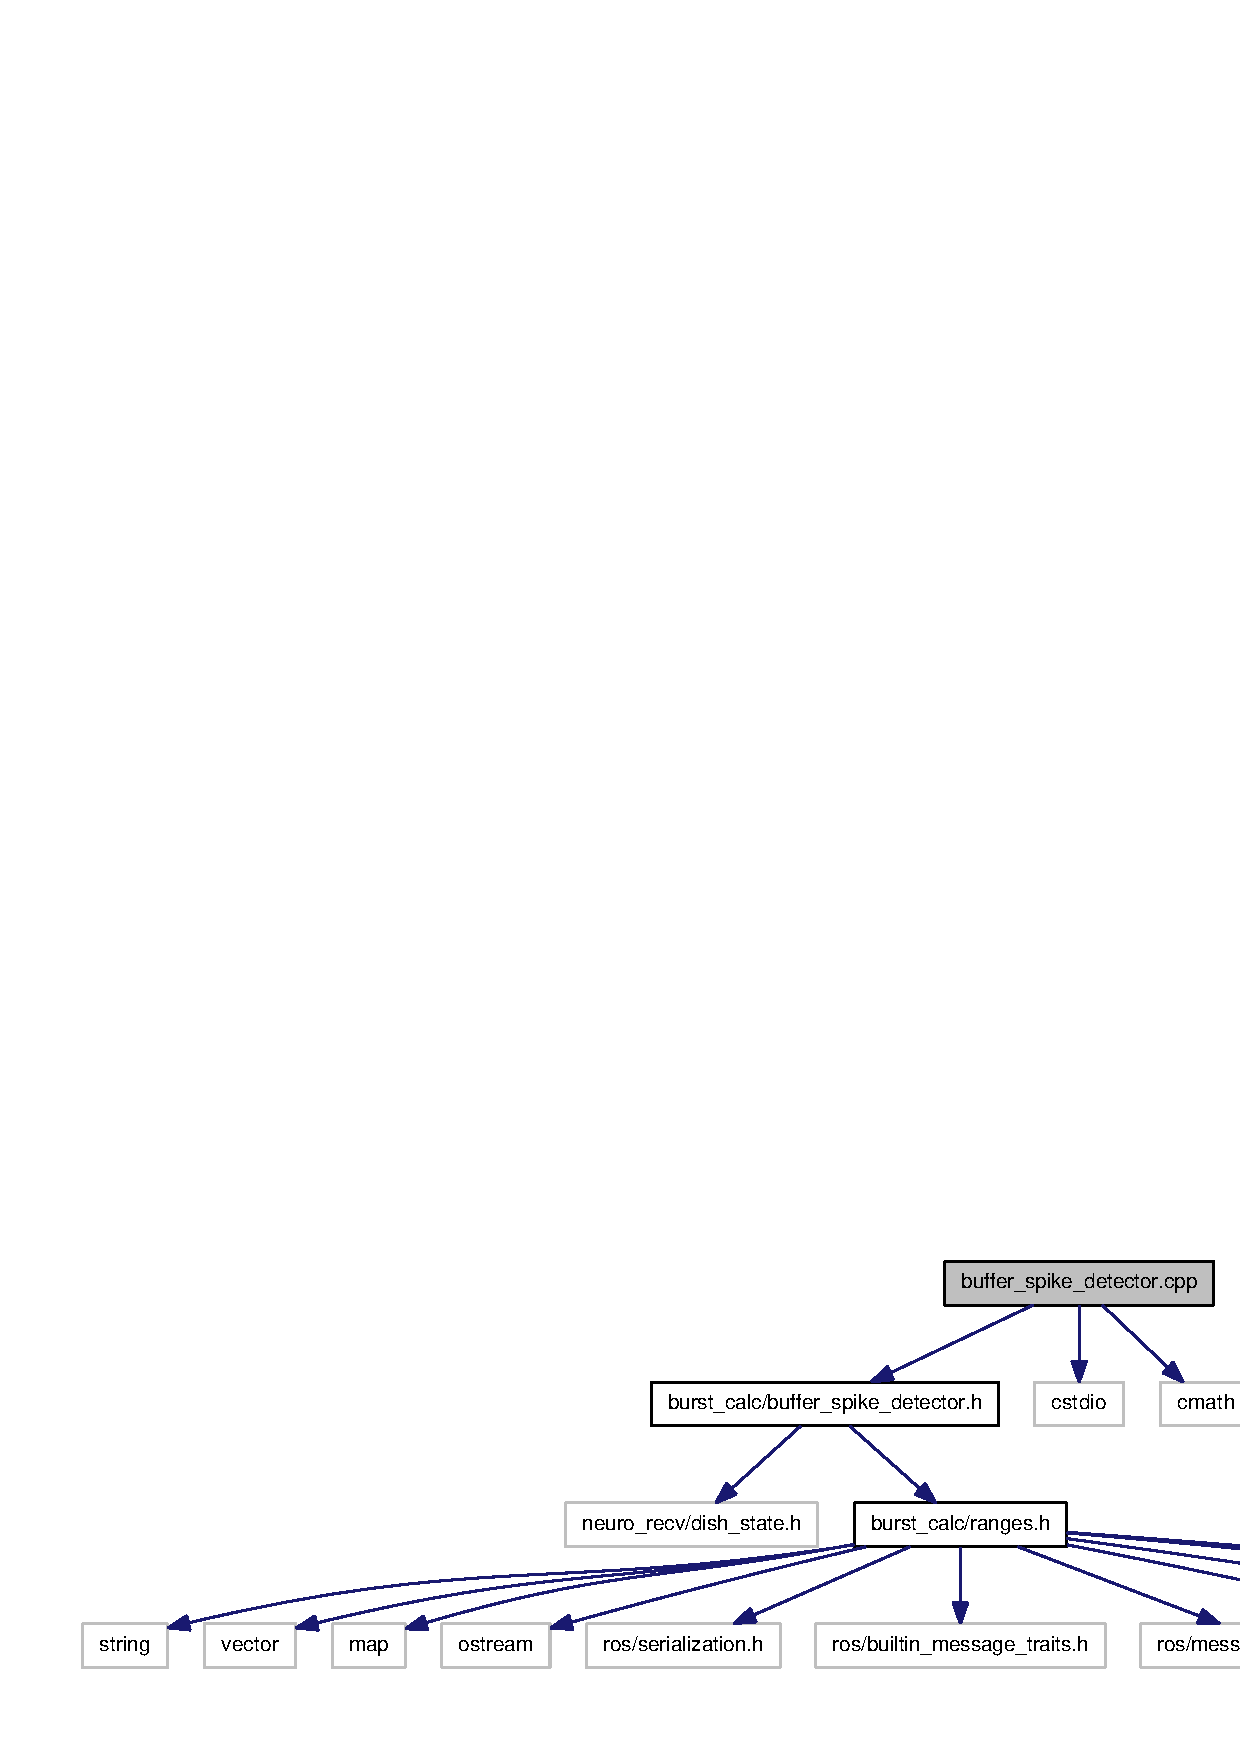
\includegraphics[width=350pt]{buffer__spike__detector_8cpp__incl}
\end{center}
\end{figure}

\section{buffer\-\_\-spike\-\_\-detector.\-h \-File \-Reference}
\label{buffer__spike__detector_8h}\index{buffer\-\_\-spike\-\_\-detector.\-h@{buffer\-\_\-spike\-\_\-detector.\-h}}
{\ttfamily \#include \char`\"{}neuro\-\_\-recv/dish\-\_\-state.\-h\char`\"{}}\*
{\ttfamily \#include \char`\"{}burst\-\_\-calc/ranges.\-h\char`\"{}}\*
\-Include dependency graph for buffer\-\_\-spike\-\_\-detector.\-h\-:\nopagebreak
\begin{figure}[H]
\begin{center}
\leavevmode
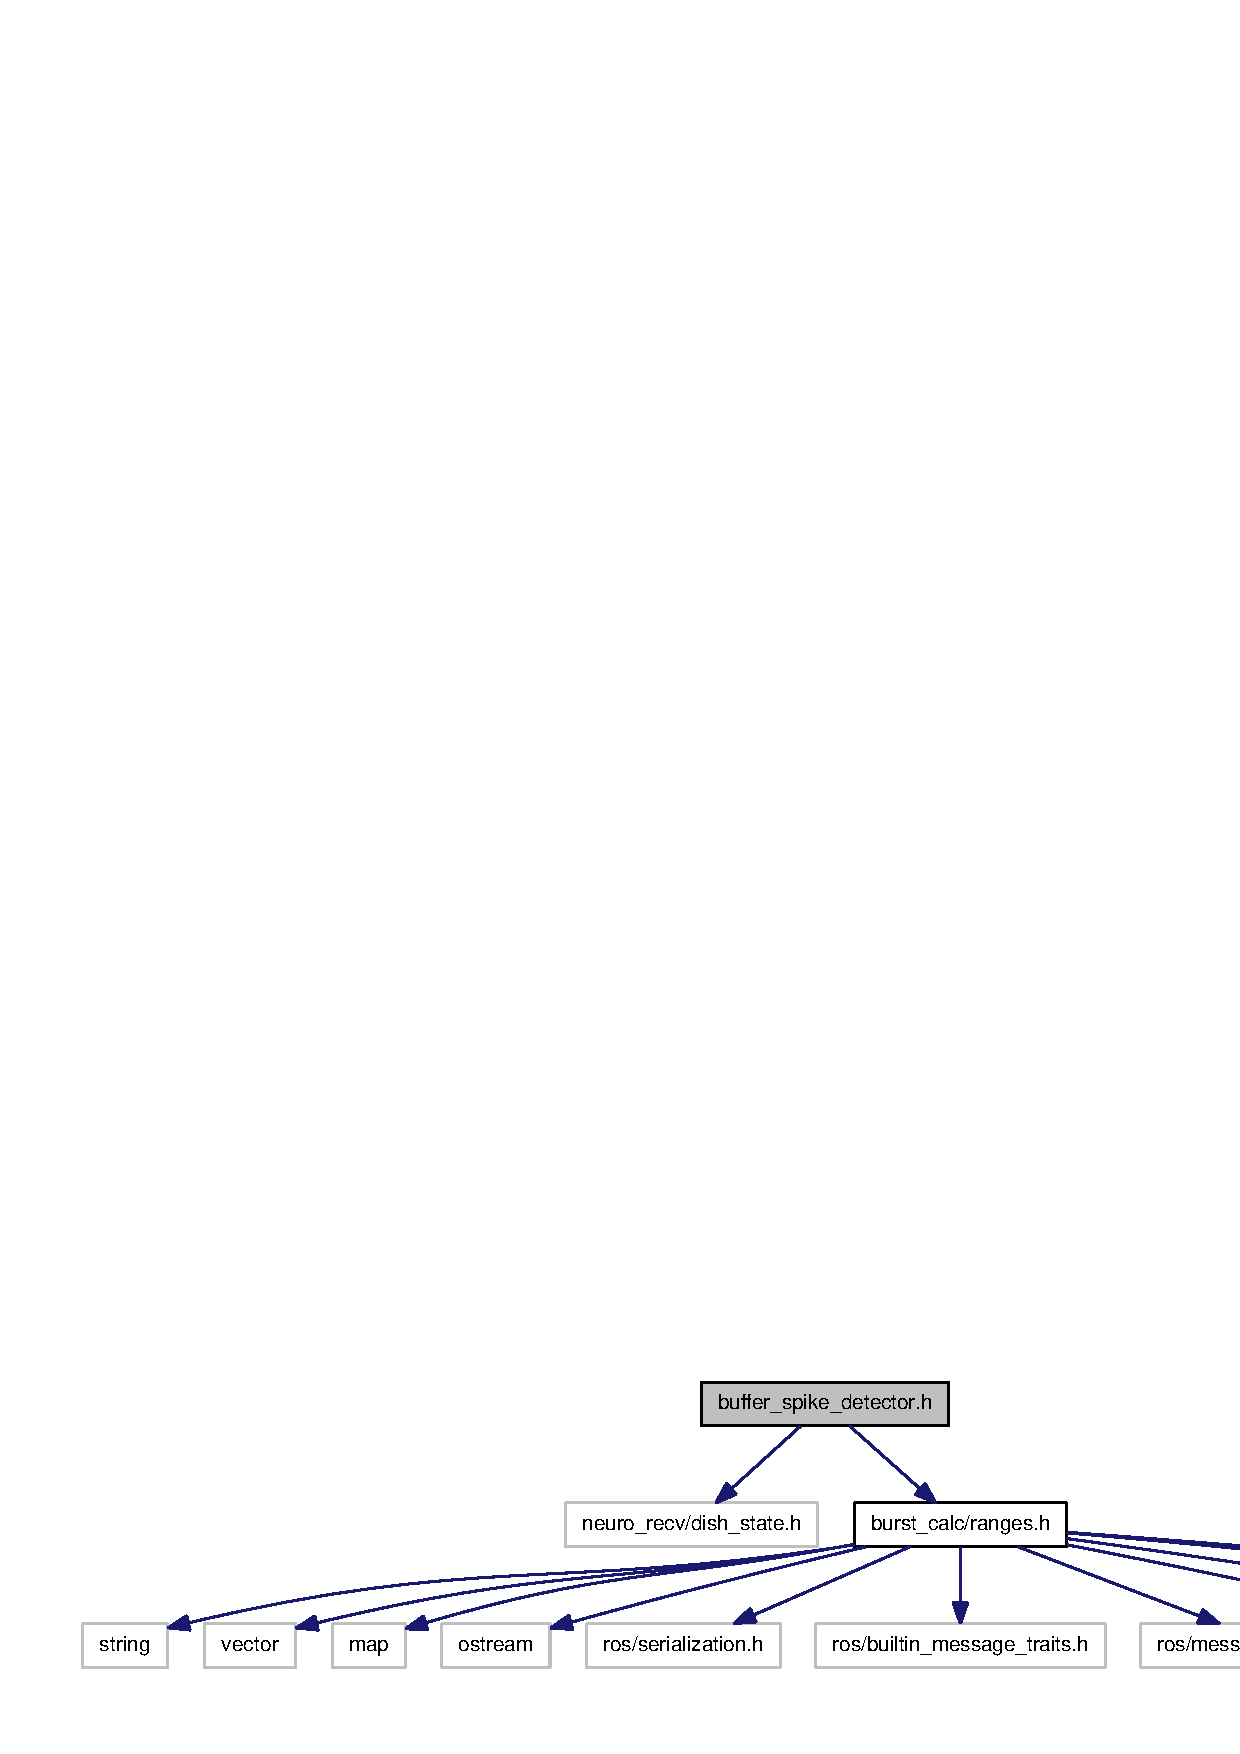
\includegraphics[width=350pt]{buffer__spike__detector_8h__incl}
\end{center}
\end{figure}
\-This graph shows which files directly or indirectly include this file\-:\nopagebreak
\begin{figure}[H]
\begin{center}
\leavevmode
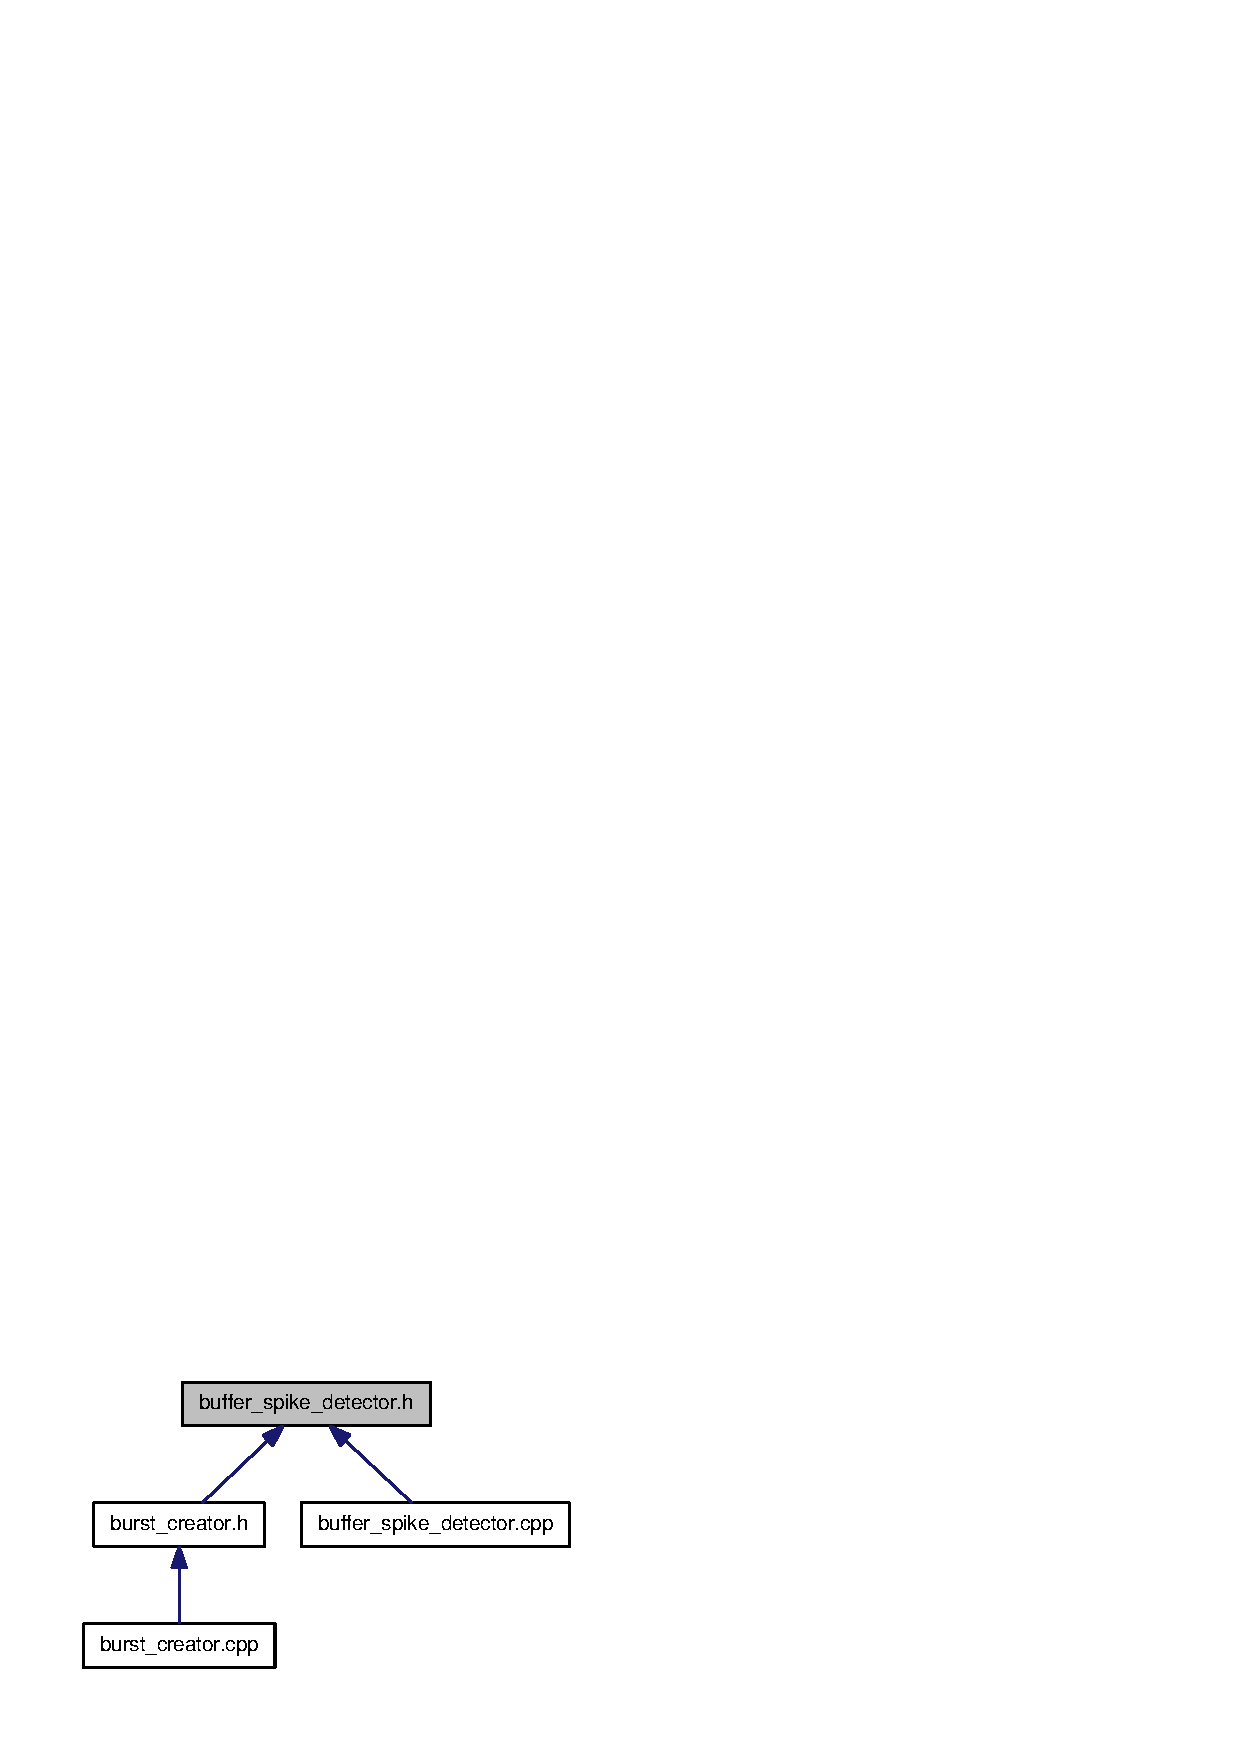
\includegraphics[width=277pt]{buffer__spike__detector_8h__dep__incl}
\end{center}
\end{figure}
\subsection*{\-Classes}
\begin{DoxyCompactItemize}
\item 
class {\bf \-Buffer\-Spike\-Detector}
\begin{DoxyCompactList}\small\item\em \-Helper class for the burst\-\_\-creator node. \end{DoxyCompactList}\end{DoxyCompactItemize}

\section{burst.\-h \-File \-Reference}
\label{burst_8h}\index{burst.\-h@{burst.\-h}}
{\ttfamily \#include $<$string$>$}\*
{\ttfamily \#include $<$vector$>$}\*
{\ttfamily \#include $<$map$>$}\*
{\ttfamily \#include $<$ostream$>$}\*
{\ttfamily \#include \char`\"{}ros/serialization.\-h\char`\"{}}\*
{\ttfamily \#include \char`\"{}ros/builtin\-\_\-message\-\_\-traits.\-h\char`\"{}}\*
{\ttfamily \#include \char`\"{}ros/message\-\_\-operations.\-h\char`\"{}}\*
{\ttfamily \#include \char`\"{}ros/time.\-h\char`\"{}}\*
{\ttfamily \#include \char`\"{}ros/macros.\-h\char`\"{}}\*
{\ttfamily \#include \char`\"{}ros/assert.\-h\char`\"{}}\*
{\ttfamily \#include \char`\"{}std\-\_\-msgs/\-Header.\-h\char`\"{}}\*
{\ttfamily \#include \char`\"{}neuro\-\_\-recv/dish\-\_\-state.\-h\char`\"{}}\*
\-Include dependency graph for burst.\-h\-:\nopagebreak
\begin{figure}[H]
\begin{center}
\leavevmode
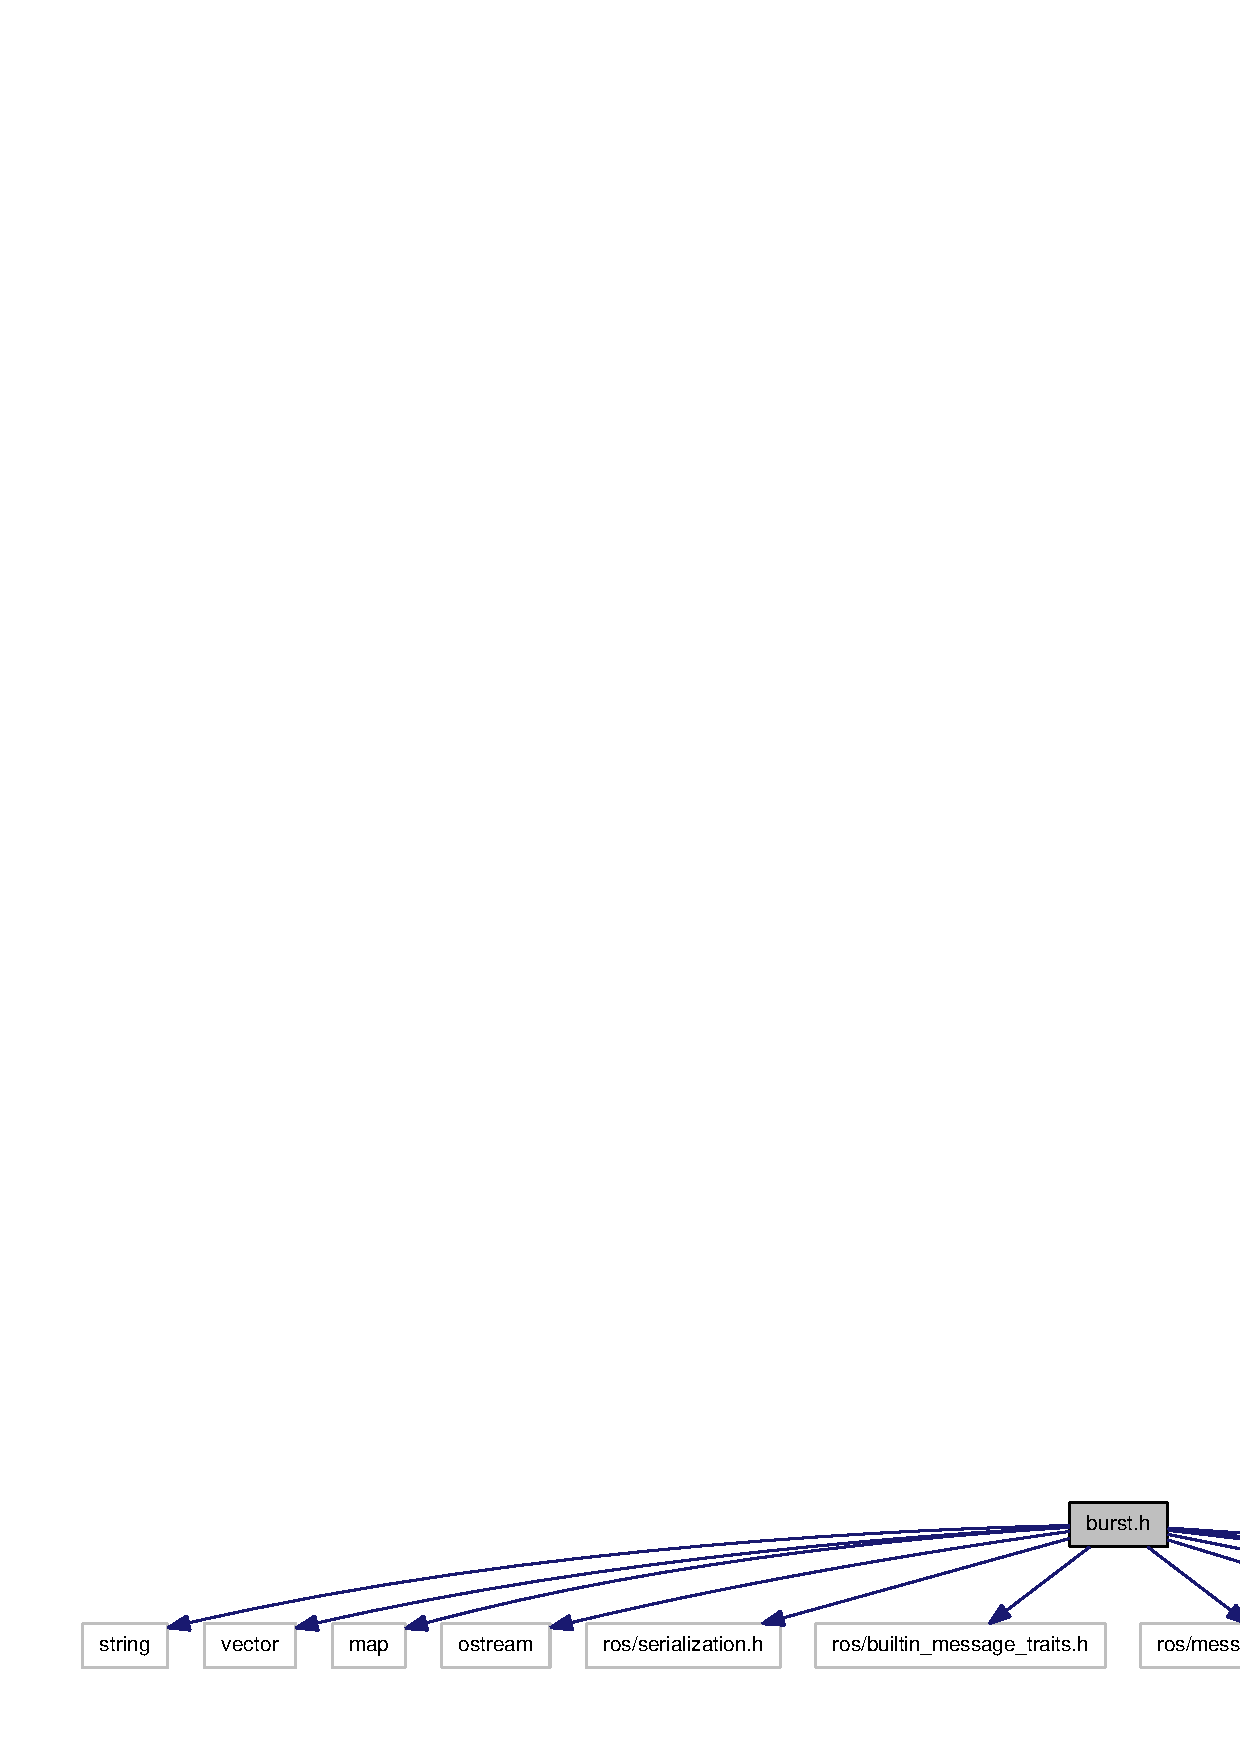
\includegraphics[width=350pt]{burst_8h__incl}
\end{center}
\end{figure}
\-This graph shows which files directly or indirectly include this file\-:\nopagebreak
\begin{figure}[H]
\begin{center}
\leavevmode
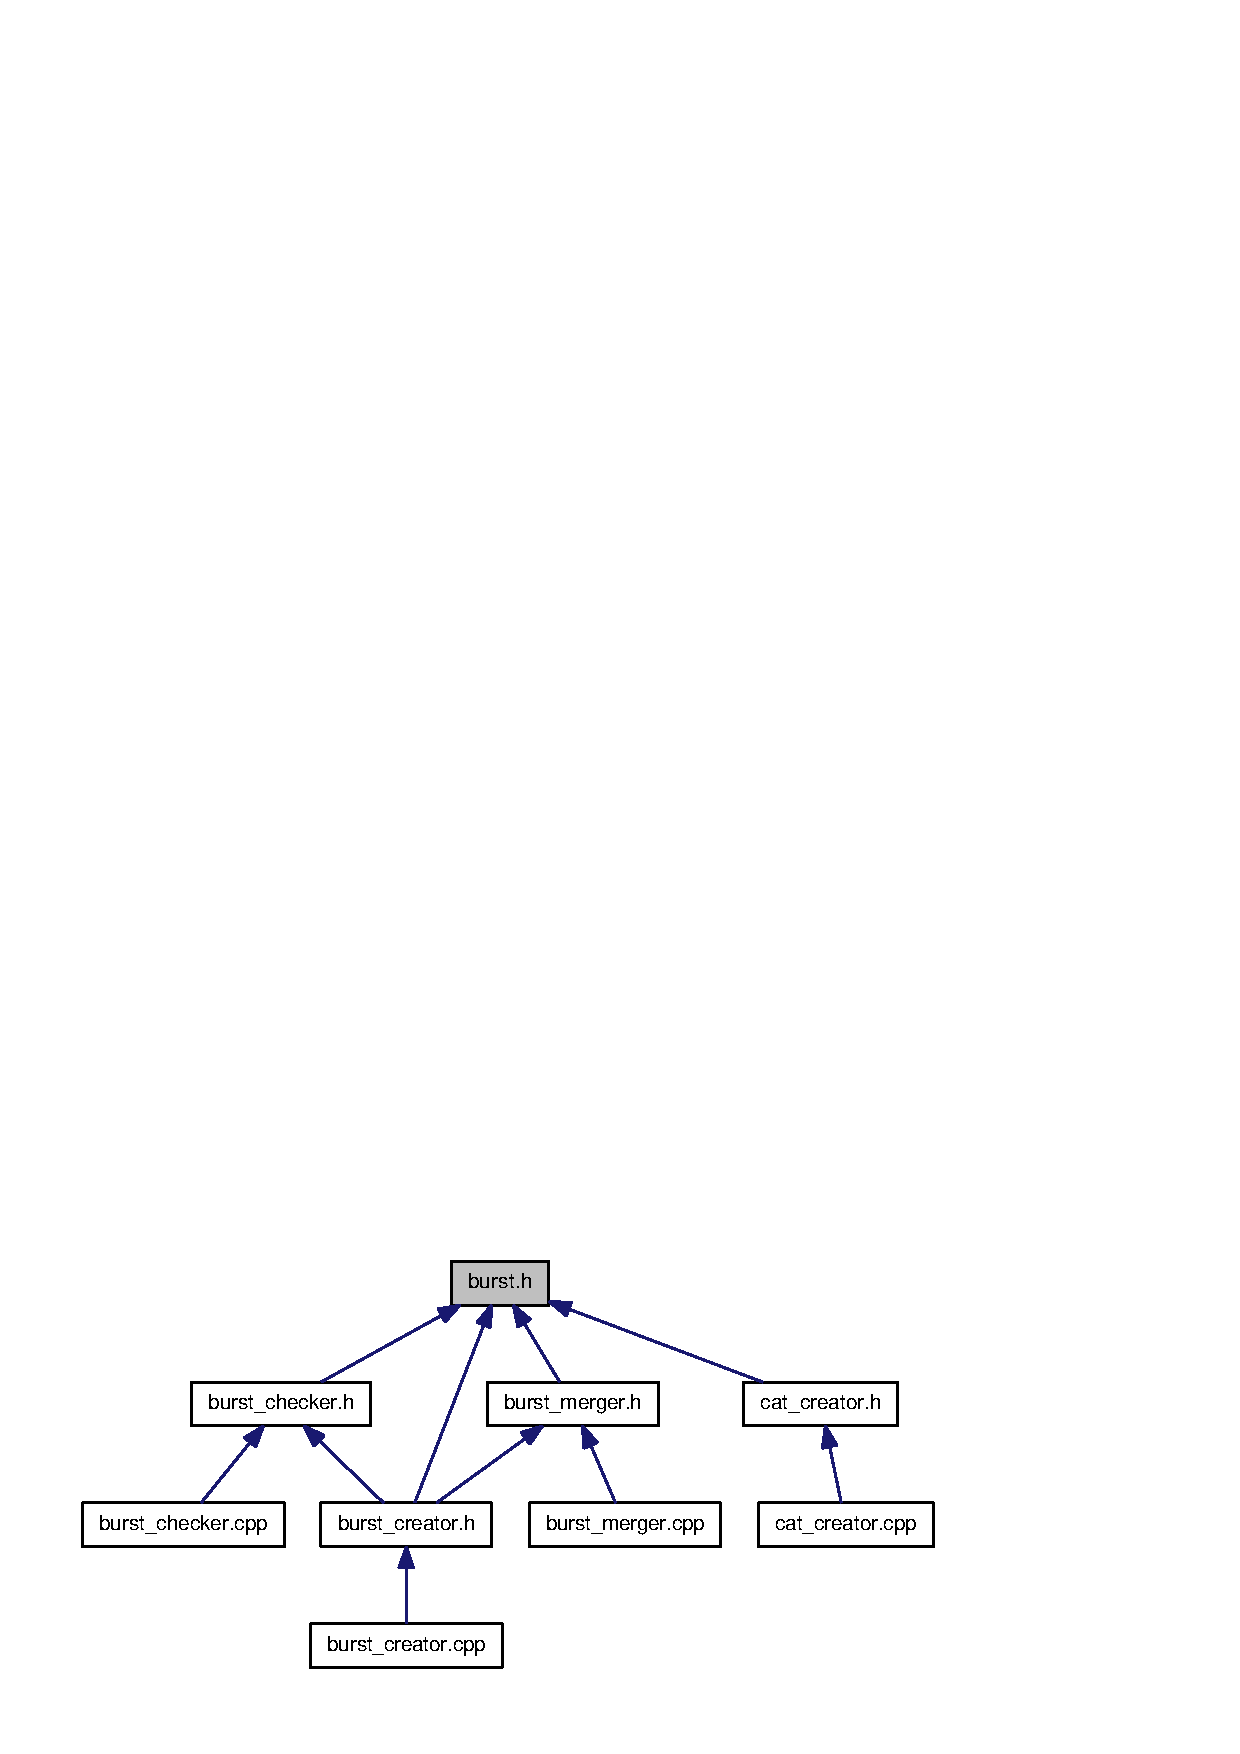
\includegraphics[width=350pt]{burst_8h__dep__incl}
\end{center}
\end{figure}
\subsection*{\-Classes}
\begin{DoxyCompactItemize}
\item 
struct {\bf burst\-\_\-calc\-::burst\-\_\-$<$ Container\-Allocator $>$}
\item 
struct {\bf ros\-::message\-\_\-traits\-::\-Data\-Type$<$ \-::burst\-\_\-calc\-::burst\-\_\-$<$ Container\-Allocator $>$ $>$}
\item 
struct {\bf ros\-::message\-\_\-traits\-::\-Definition$<$ \-::burst\-\_\-calc\-::burst\-\_\-$<$ Container\-Allocator $>$ $>$}
\item 
struct {\bf ros\-::message\-\_\-traits\-::\-Has\-Header$<$ \-::burst\-\_\-calc\-::burst\-\_\-$<$ Container\-Allocator $>$ $>$}
\item 
struct {\bf ros\-::message\-\_\-traits\-::\-Has\-Header$<$ const \-::burst\-\_\-calc\-::burst\-\_\-$<$ Container\-Allocator $>$ $>$}
\item 
struct {\bf ros\-::message\-\_\-traits\-::\-Is\-Message$<$ \-::burst\-\_\-calc\-::burst\-\_\-$<$ Container\-Allocator $>$ $>$}
\item 
struct {\bf ros\-::message\-\_\-traits\-::\-Is\-Message$<$ \-::burst\-\_\-calc\-::burst\-\_\-$<$ Container\-Allocator $>$const  $>$}
\item 
struct {\bf ros\-::message\-\_\-traits\-::\-M\-D5\-Sum$<$ \-::burst\-\_\-calc\-::burst\-\_\-$<$ Container\-Allocator $>$ $>$}
\item 
struct {\bf ros\-::message\-\_\-operations\-::\-Printer$<$ \-::burst\-\_\-calc\-::burst\-\_\-$<$ Container\-Allocator $>$ $>$}
\item 
struct {\bf ros\-::serialization\-::\-Serializer$<$ \-::burst\-\_\-calc\-::burst\-\_\-$<$ Container\-Allocator $>$ $>$}
\end{DoxyCompactItemize}
\subsection*{\-Namespaces}
\begin{DoxyCompactItemize}
\item 
namespace {\bf burst\-\_\-calc}
\item 
namespace {\bf ros}
\item 
namespace {\bf ros\-::message\-\_\-operations}
\item 
namespace {\bf ros\-::message\-\_\-traits}
\item 
namespace {\bf ros\-::serialization}
\end{DoxyCompactItemize}
\subsection*{\-Typedefs}
\begin{DoxyCompactItemize}
\item 
typedef \-::{\bf burst\-\_\-calc\-::burst\-\_\-}\*
$<$ std\-::allocator$<$ void $>$ $>$ {\bf burst\-\_\-calc\-::burst}
\item 
typedef boost\-::shared\-\_\-ptr\*
$<$ \-::{\bf burst\-\_\-calc\-::burst} const  $>$ {\bf burst\-\_\-calc\-::burst\-Const\-Ptr}
\item 
typedef boost\-::shared\-\_\-ptr\*
$<$ \-::{\bf burst\-\_\-calc\-::burst} $>$ {\bf burst\-\_\-calc\-::burst\-Ptr}
\end{DoxyCompactItemize}
\subsection*{\-Functions}
\begin{DoxyCompactItemize}
\item 
{\footnotesize template$<$typename Container\-Allocator $>$ }\\std\-::ostream \& {\bf burst\-\_\-calc\-::operator$<$$<$} (std\-::ostream \&s, const \-::{\bf burst\-\_\-calc\-::burst\-\_\-}$<$ \-Container\-Allocator $>$ \&v)
\end{DoxyCompactItemize}

\section{burst\-\_\-checker.\-cpp \-File \-Reference}
\label{burst__checker_8cpp}\index{burst\-\_\-checker.\-cpp@{burst\-\_\-checker.\-cpp}}
{\ttfamily \#include \char`\"{}burst\-\_\-calc/burst\-\_\-checker.\-h\char`\"{}}\*
{\ttfamily \#include $<$cstdio$>$}\*
\-Include dependency graph for burst\-\_\-checker.\-cpp\-:\nopagebreak
\begin{figure}[H]
\begin{center}
\leavevmode
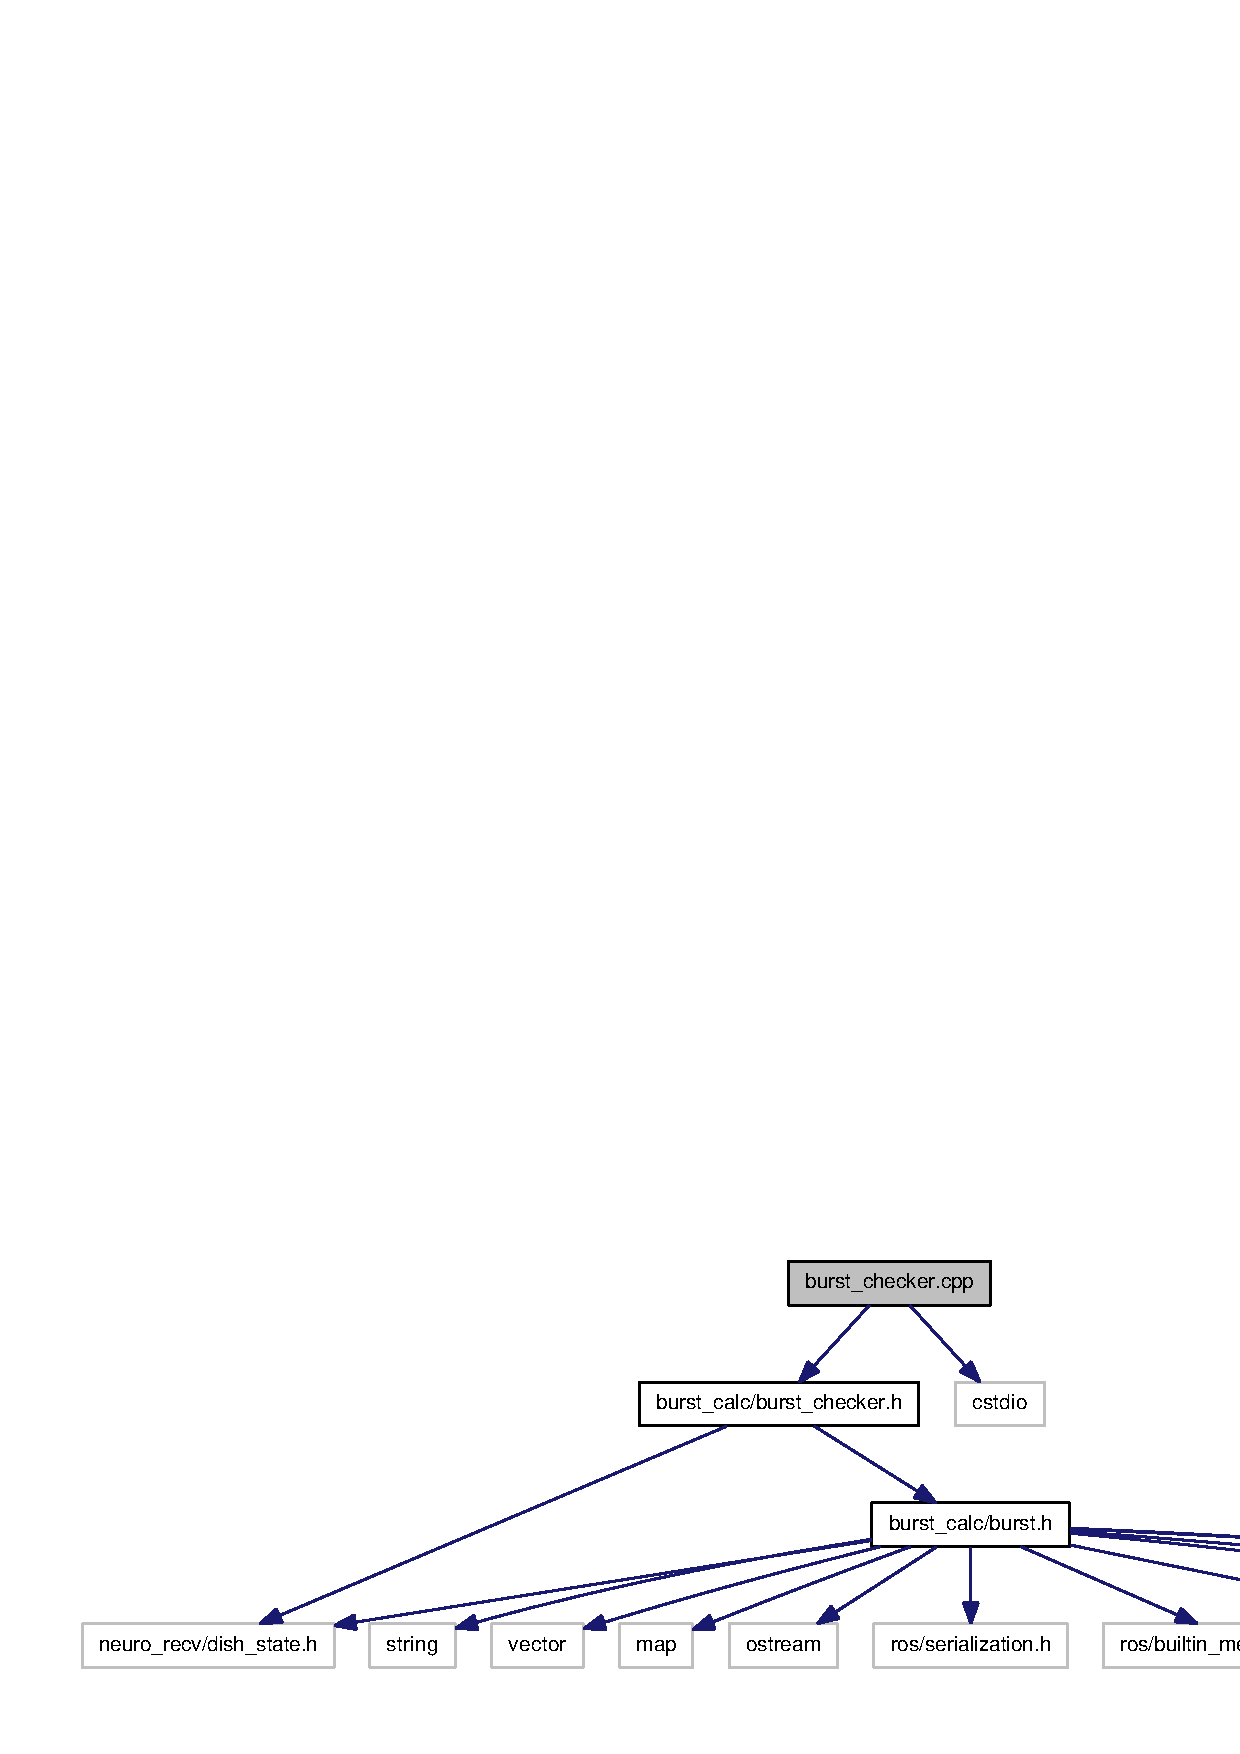
\includegraphics[width=350pt]{burst__checker_8cpp__incl}
\end{center}
\end{figure}

\section{burst\-\_\-checker.\-h \-File \-Reference}
\label{burst__checker_8h}\index{burst\-\_\-checker.\-h@{burst\-\_\-checker.\-h}}
{\ttfamily \#include \char`\"{}neuro\-\_\-recv/dish\-\_\-state.\-h\char`\"{}}\*
{\ttfamily \#include \char`\"{}burst\-\_\-calc/burst.\-h\char`\"{}}\*
\-Include dependency graph for burst\-\_\-checker.\-h\-:\nopagebreak
\begin{figure}[H]
\begin{center}
\leavevmode
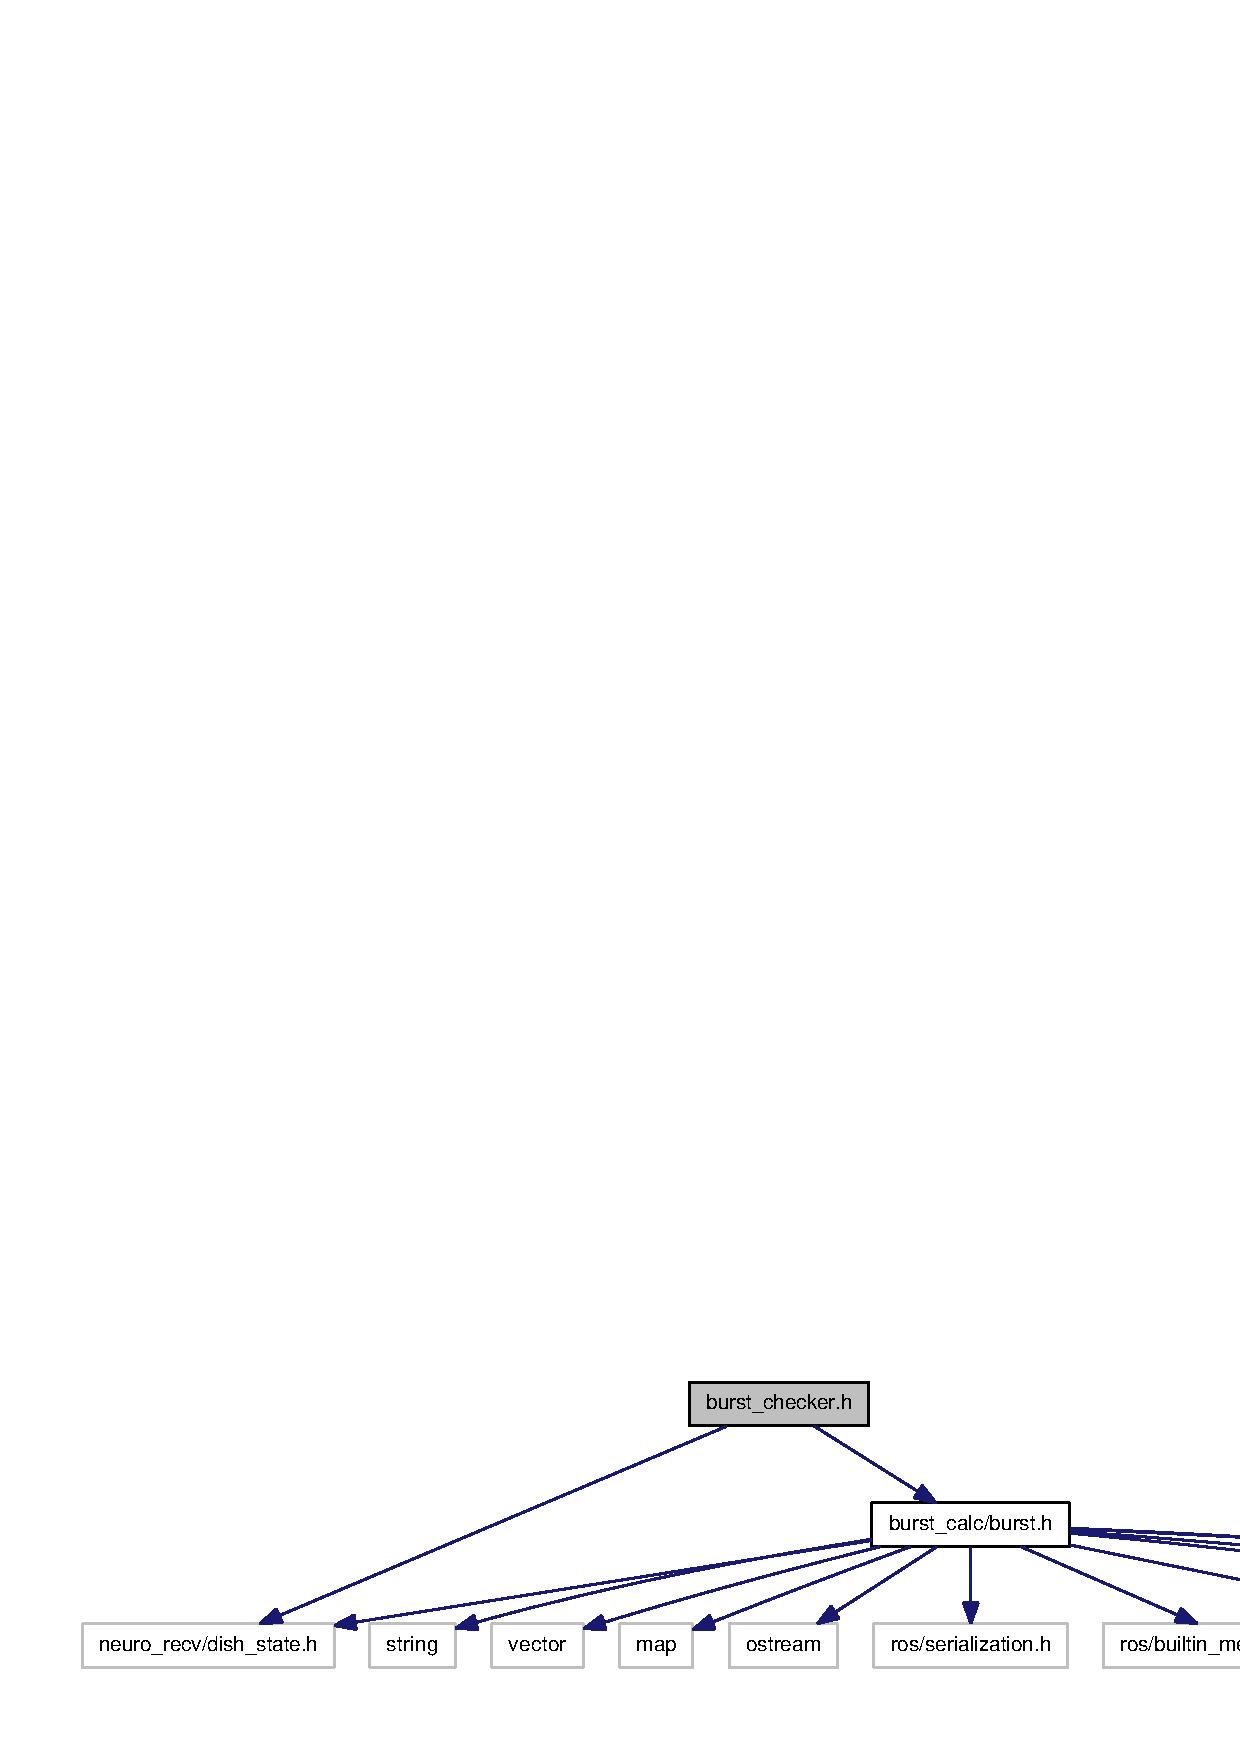
\includegraphics[width=350pt]{burst__checker_8h__incl}
\end{center}
\end{figure}
\-This graph shows which files directly or indirectly include this file\-:\nopagebreak
\begin{figure}[H]
\begin{center}
\leavevmode
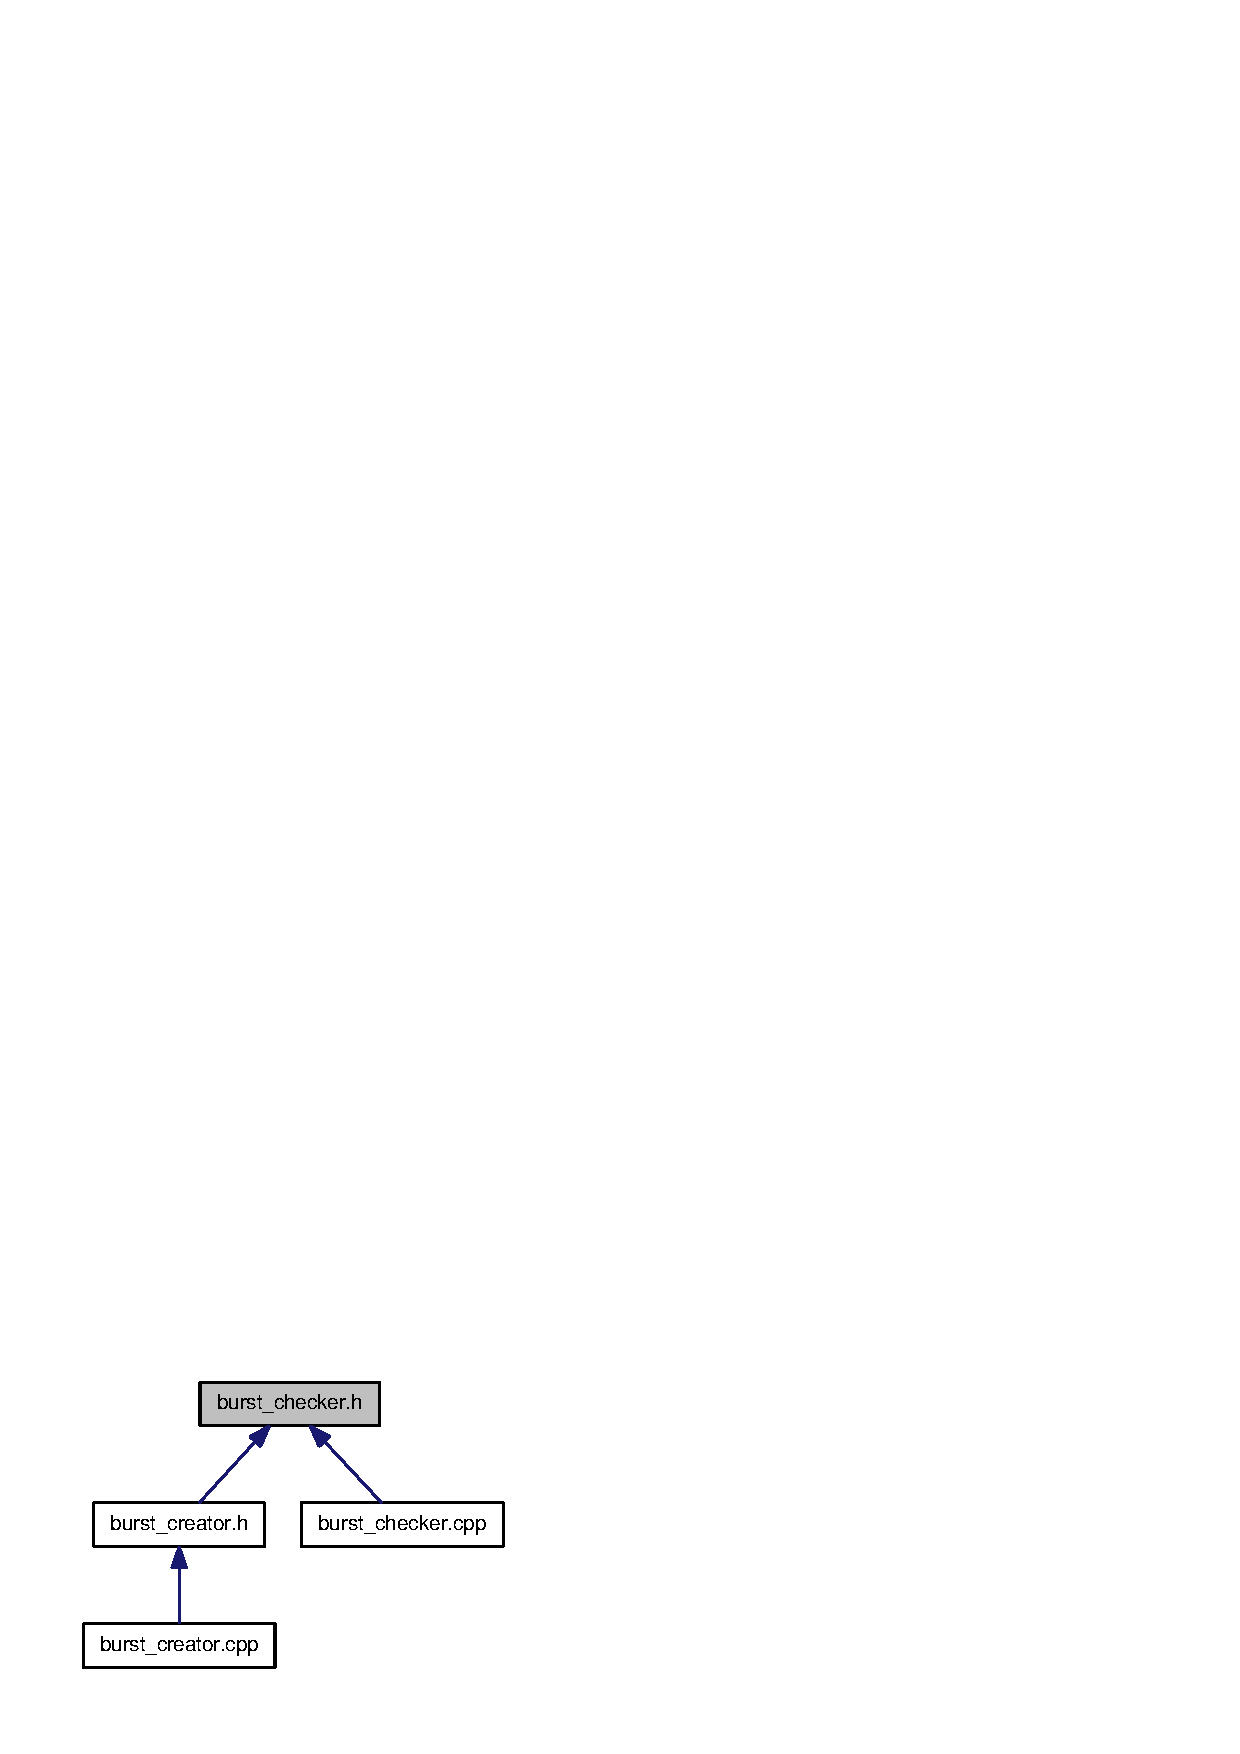
\includegraphics[width=245pt]{burst__checker_8h__dep__incl}
\end{center}
\end{figure}
\subsection*{\-Classes}
\begin{DoxyCompactItemize}
\item 
class {\bf \-Burst\-Checker}
\begin{DoxyCompactList}\small\item\em \-Helper class for the burst\-\_\-creator node. \end{DoxyCompactList}\end{DoxyCompactItemize}

\section{burst\-\_\-creator.\-cpp \-File \-Reference}
\label{burst__creator_8cpp}\index{burst\-\_\-creator.\-cpp@{burst\-\_\-creator.\-cpp}}
{\ttfamily \#include \char`\"{}burst\-\_\-calc/burst\-\_\-creator.\-h\char`\"{}}\*
{\ttfamily \#include \char`\"{}burst\-\_\-calc/ranges.\-h\char`\"{}}\*
{\ttfamily \#include \char`\"{}time\-\_\-server/time\-\_\-srv.\-h\char`\"{}}\*
{\ttfamily \#include $<$cstdio$>$}\*
\-Include dependency graph for burst\-\_\-creator.\-cpp\-:\nopagebreak
\begin{figure}[H]
\begin{center}
\leavevmode
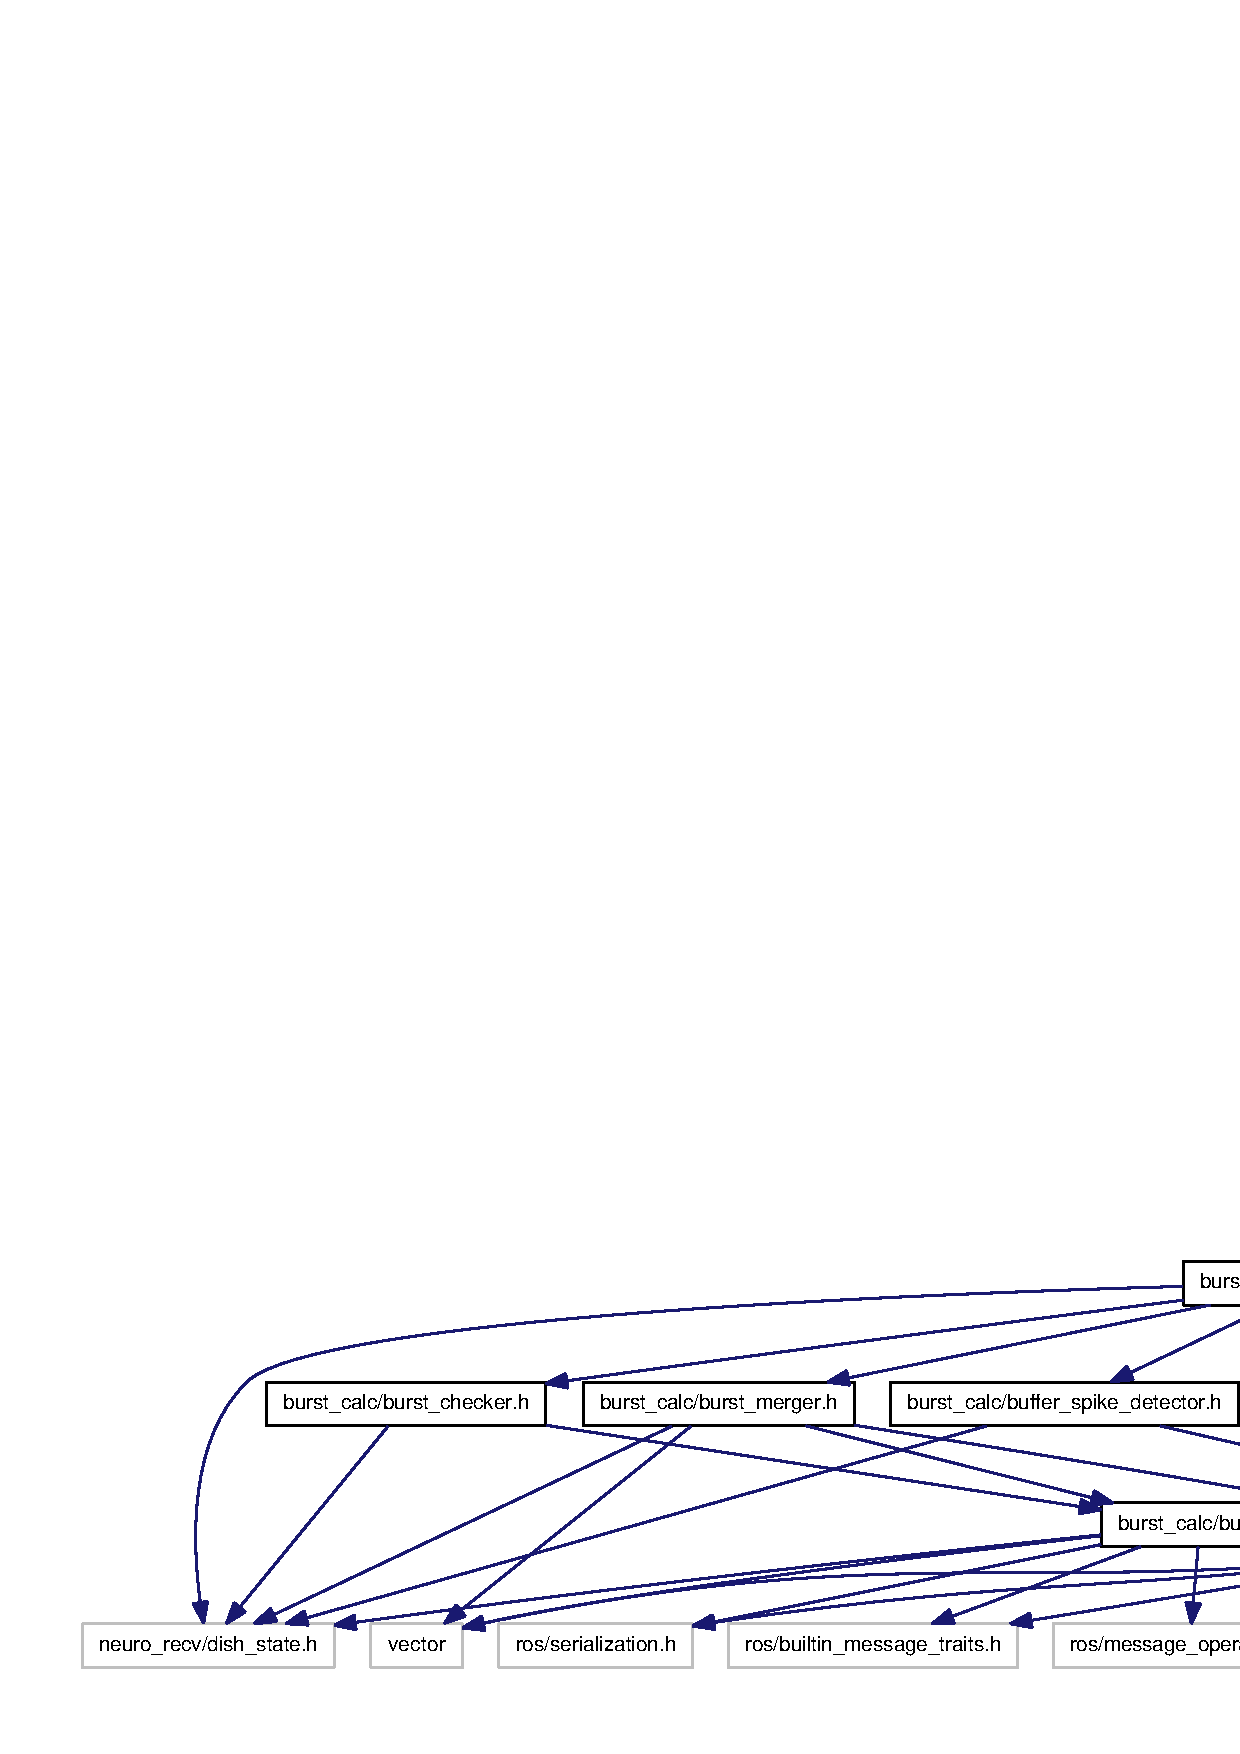
\includegraphics[width=350pt]{burst__creator_8cpp__incl}
\end{center}
\end{figure}
\subsection*{\-Functions}
\begin{DoxyCompactItemize}
\item 
int {\bf main} (int argc, char $\ast$$\ast$argv)
\begin{DoxyCompactList}\small\item\em \-Creates an instance of the node. \end{DoxyCompactList}\end{DoxyCompactItemize}


\subsection{\-Function \-Documentation}
\index{burst\-\_\-creator.\-cpp@{burst\-\_\-creator.\-cpp}!main@{main}}
\index{main@{main}!burst_creator.cpp@{burst\-\_\-creator.\-cpp}}
\subsubsection[{main}]{\setlength{\rightskip}{0pt plus 5cm}int {\bf main} (
\begin{DoxyParamCaption}
\item[{int}]{argc, }
\item[{char $\ast$$\ast$}]{argv}
\end{DoxyParamCaption}
)}\label{burst__creator_8cpp_a3c04138a5bfe5d72780bb7e82a18e627}


\-Creates an instance of the node. 



\-Definition at line 247 of file burst\-\_\-creator.\-cpp.


\section{burst\-\_\-creator.\-h \-File \-Reference}
\label{burst__creator_8h}\index{burst\-\_\-creator.\-h@{burst\-\_\-creator.\-h}}
{\ttfamily \#include \char`\"{}ros/ros.\-h\char`\"{}}\*
{\ttfamily \#include \char`\"{}burst\-\_\-calc/buffer\-\_\-spike\-\_\-detector.\-h\char`\"{}}\*
{\ttfamily \#include \char`\"{}burst\-\_\-calc/burst\-\_\-checker.\-h\char`\"{}}\*
{\ttfamily \#include \char`\"{}burst\-\_\-calc/burst\-\_\-merger.\-h\char`\"{}}\*
{\ttfamily \#include \char`\"{}burst\-\_\-calc/burst.\-h\char`\"{}}\*
{\ttfamily \#include \char`\"{}neuro\-\_\-recv/dish\-\_\-state.\-h\char`\"{}}\*
{\ttfamily \#include $<$queue$>$}\*
{\ttfamily \#include $<$string$>$}\*
\-Include dependency graph for burst\-\_\-creator.\-h\-:\nopagebreak
\begin{figure}[H]
\begin{center}
\leavevmode
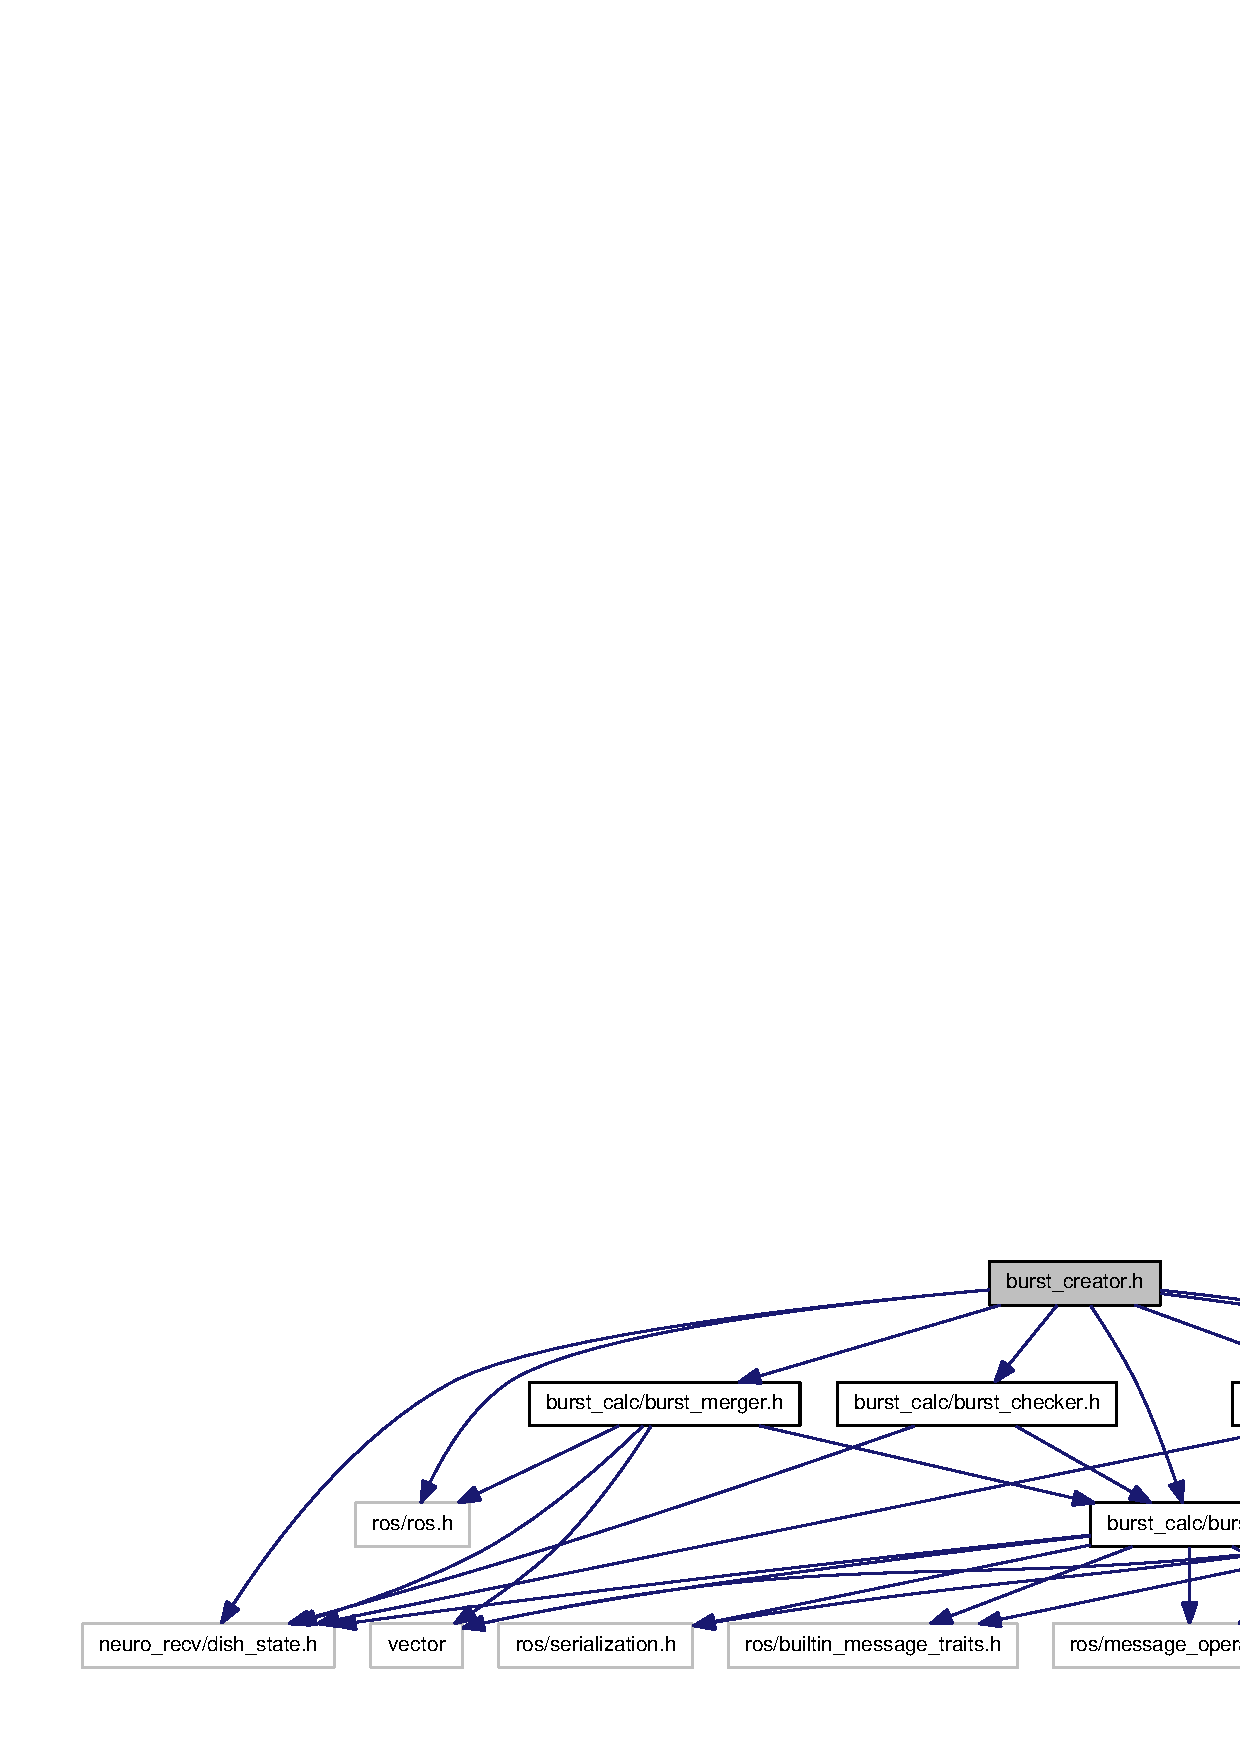
\includegraphics[width=350pt]{burst__creator_8h__incl}
\end{center}
\end{figure}
\-This graph shows which files directly or indirectly include this file\-:\nopagebreak
\begin{figure}[H]
\begin{center}
\leavevmode
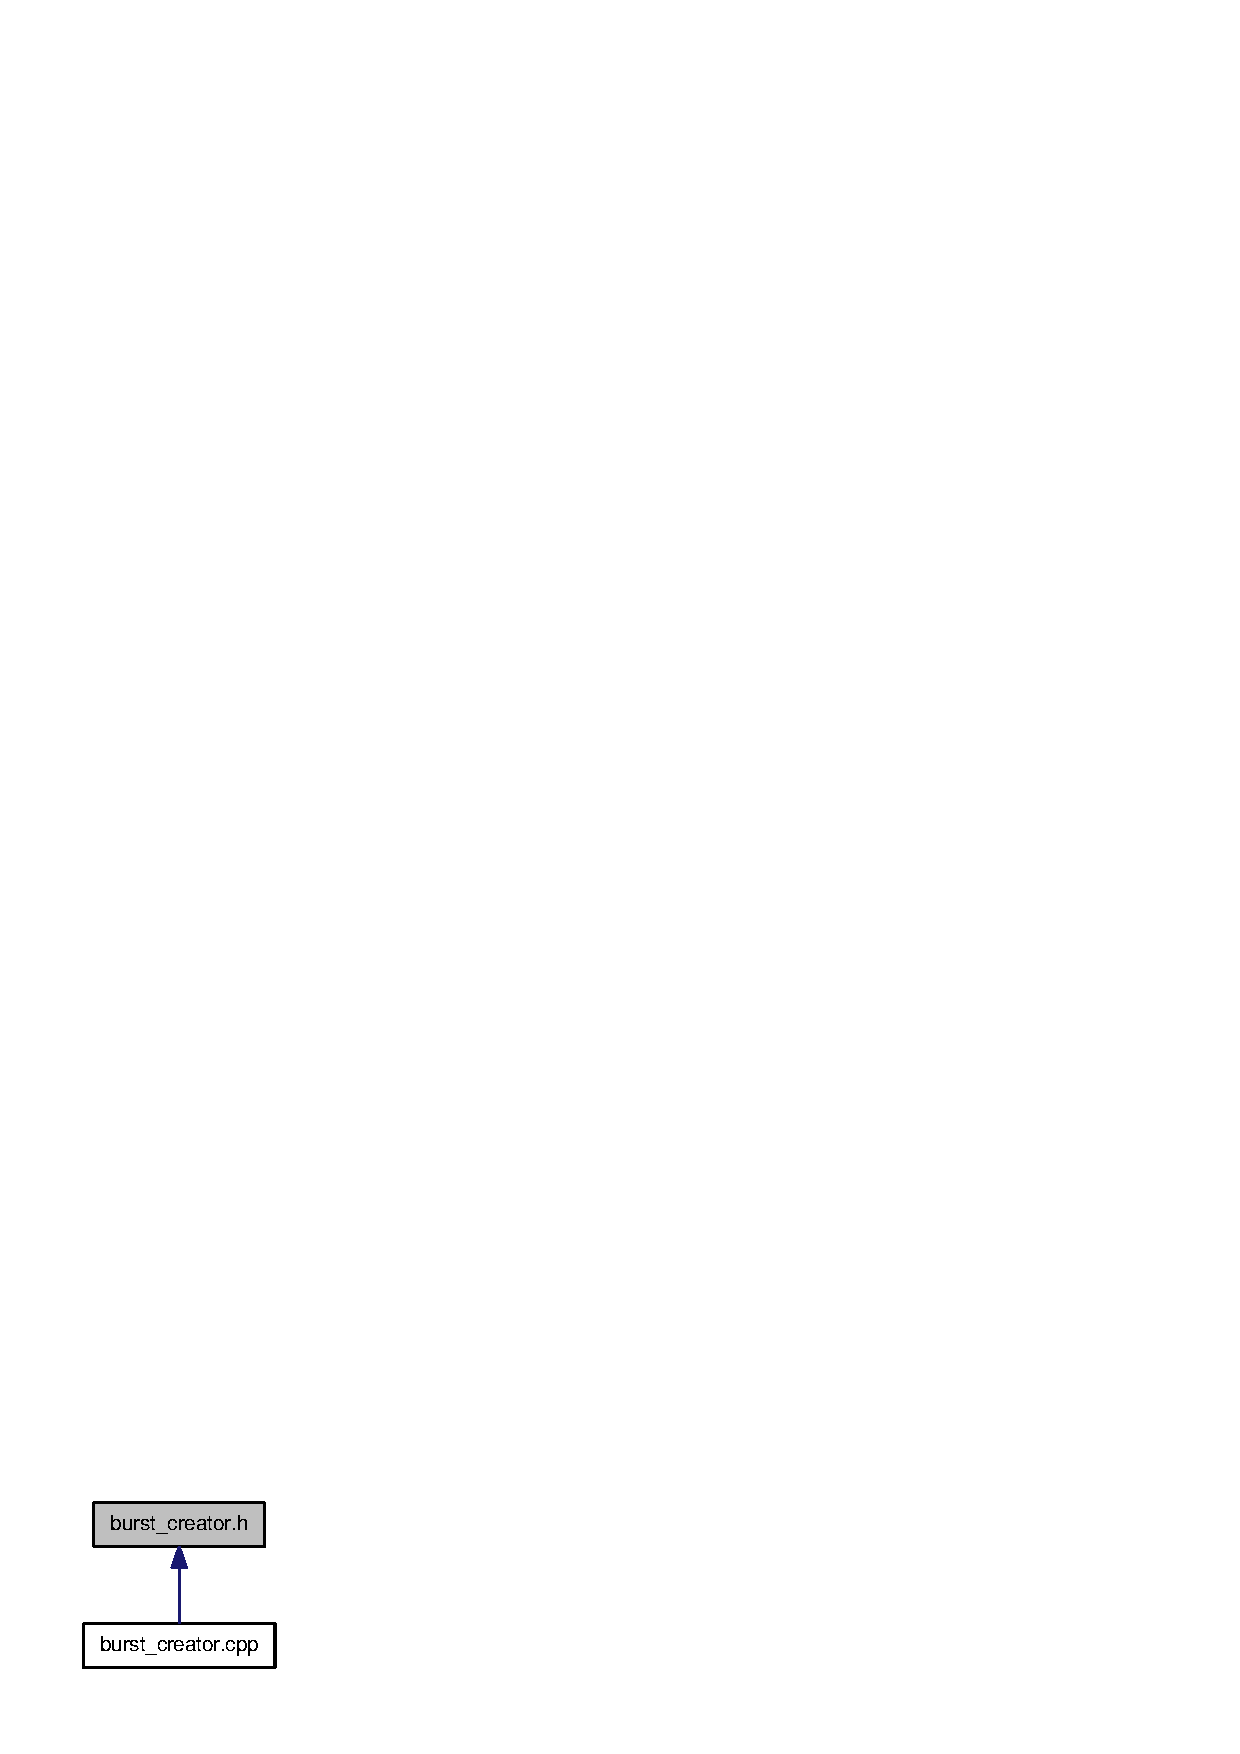
\includegraphics[width=136pt]{burst__creator_8h__dep__incl}
\end{center}
\end{figure}
\subsection*{\-Classes}
\begin{DoxyCompactItemize}
\item 
class {\bf \-Burst\-Creator}
\begin{DoxyCompactList}\small\item\em \-Node for creating bursts. \end{DoxyCompactList}\end{DoxyCompactItemize}

\section{burst\-\_\-merger.\-cpp \-File \-Reference}
\label{burst__merger_8cpp}\index{burst\-\_\-merger.\-cpp@{burst\-\_\-merger.\-cpp}}
{\ttfamily \#include \char`\"{}burst\-\_\-calc/burst\-\_\-merger.\-h\char`\"{}}\*
{\ttfamily \#include $<$cstdio$>$}\*
\-Include dependency graph for burst\-\_\-merger.\-cpp\-:\nopagebreak
\begin{figure}[H]
\begin{center}
\leavevmode
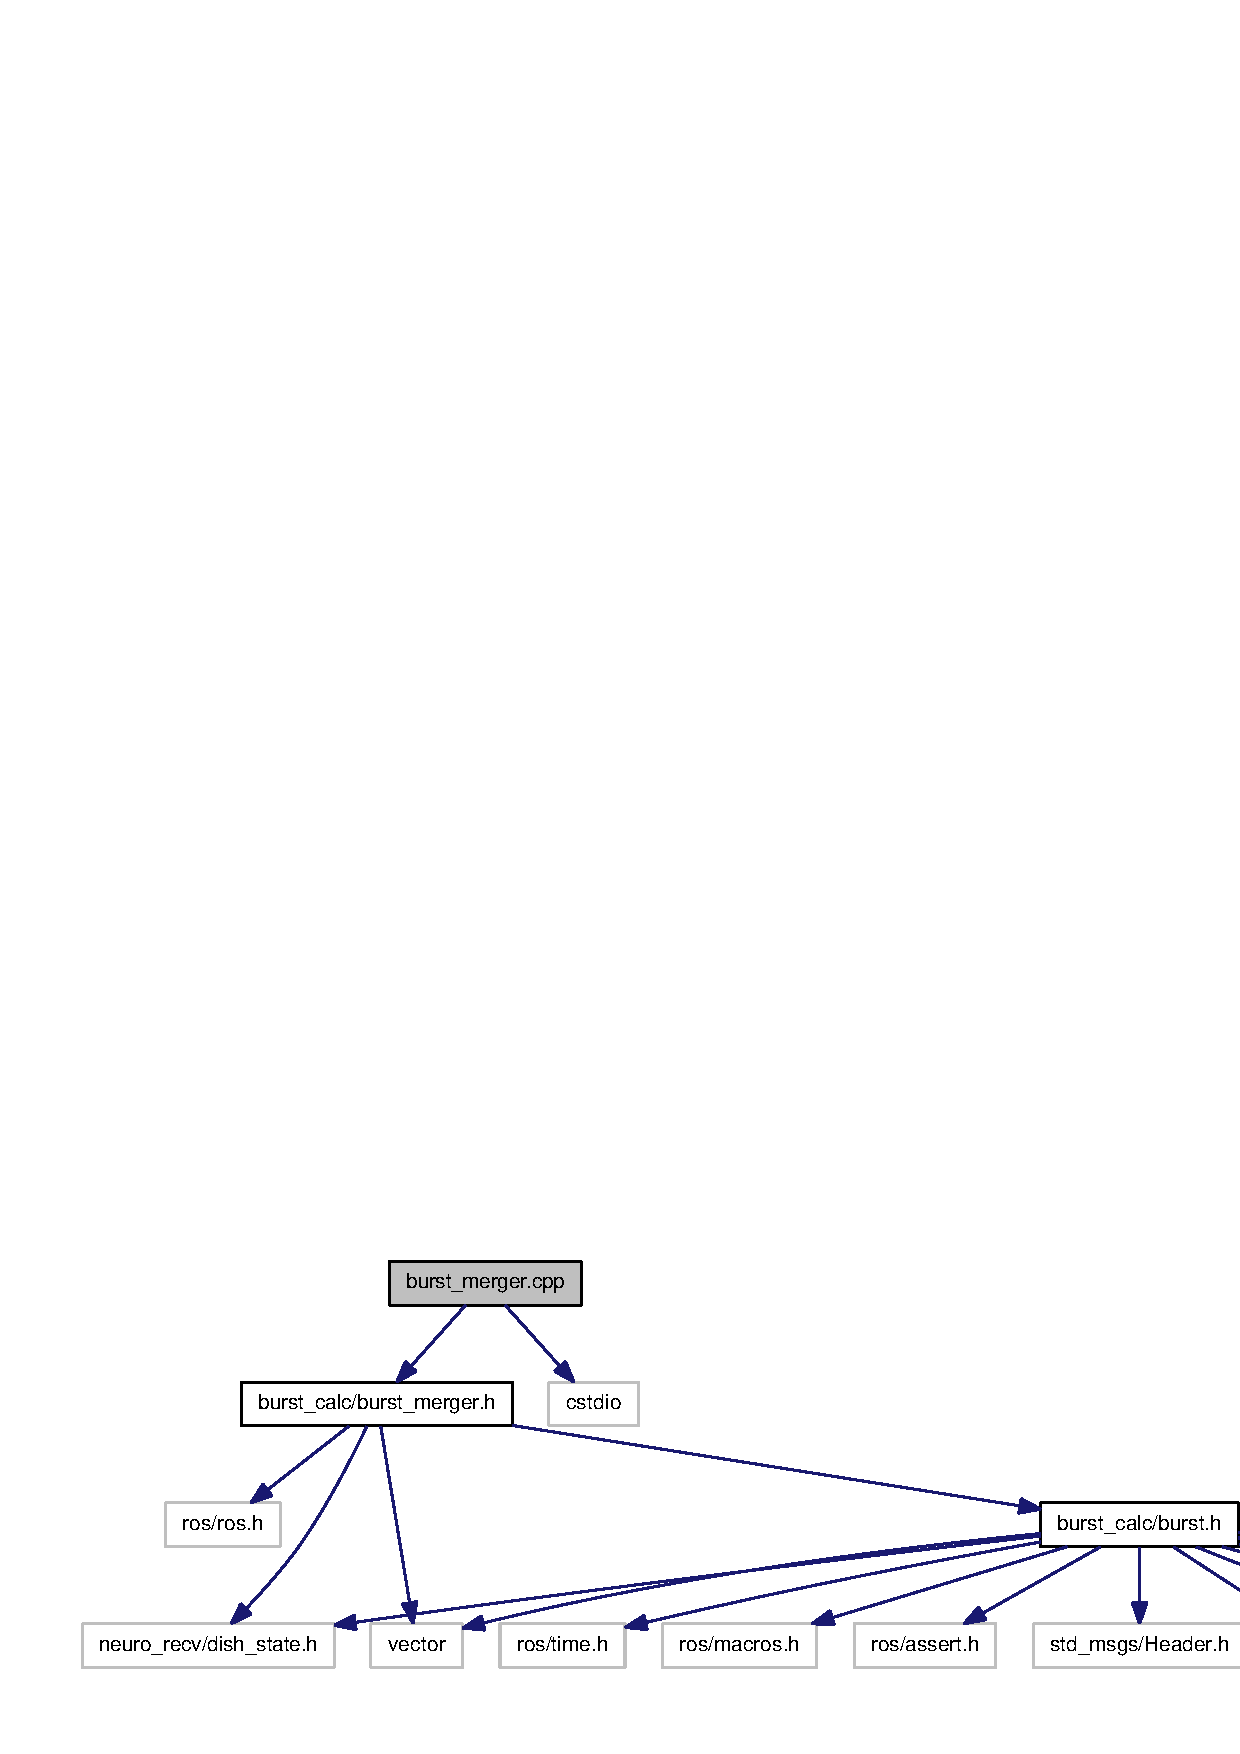
\includegraphics[width=350pt]{burst__merger_8cpp__incl}
\end{center}
\end{figure}

\section{burst\-\_\-merger.\-h \-File \-Reference}
\label{burst__merger_8h}\index{burst\-\_\-merger.\-h@{burst\-\_\-merger.\-h}}
{\ttfamily \#include \char`\"{}ros/ros.\-h\char`\"{}}\*
{\ttfamily \#include \char`\"{}neuro\-\_\-recv/dish\-\_\-state.\-h\char`\"{}}\*
{\ttfamily \#include \char`\"{}burst\-\_\-calc/burst.\-h\char`\"{}}\*
{\ttfamily \#include $<$vector$>$}\*
\-Include dependency graph for burst\-\_\-merger.\-h\-:\nopagebreak
\begin{figure}[H]
\begin{center}
\leavevmode
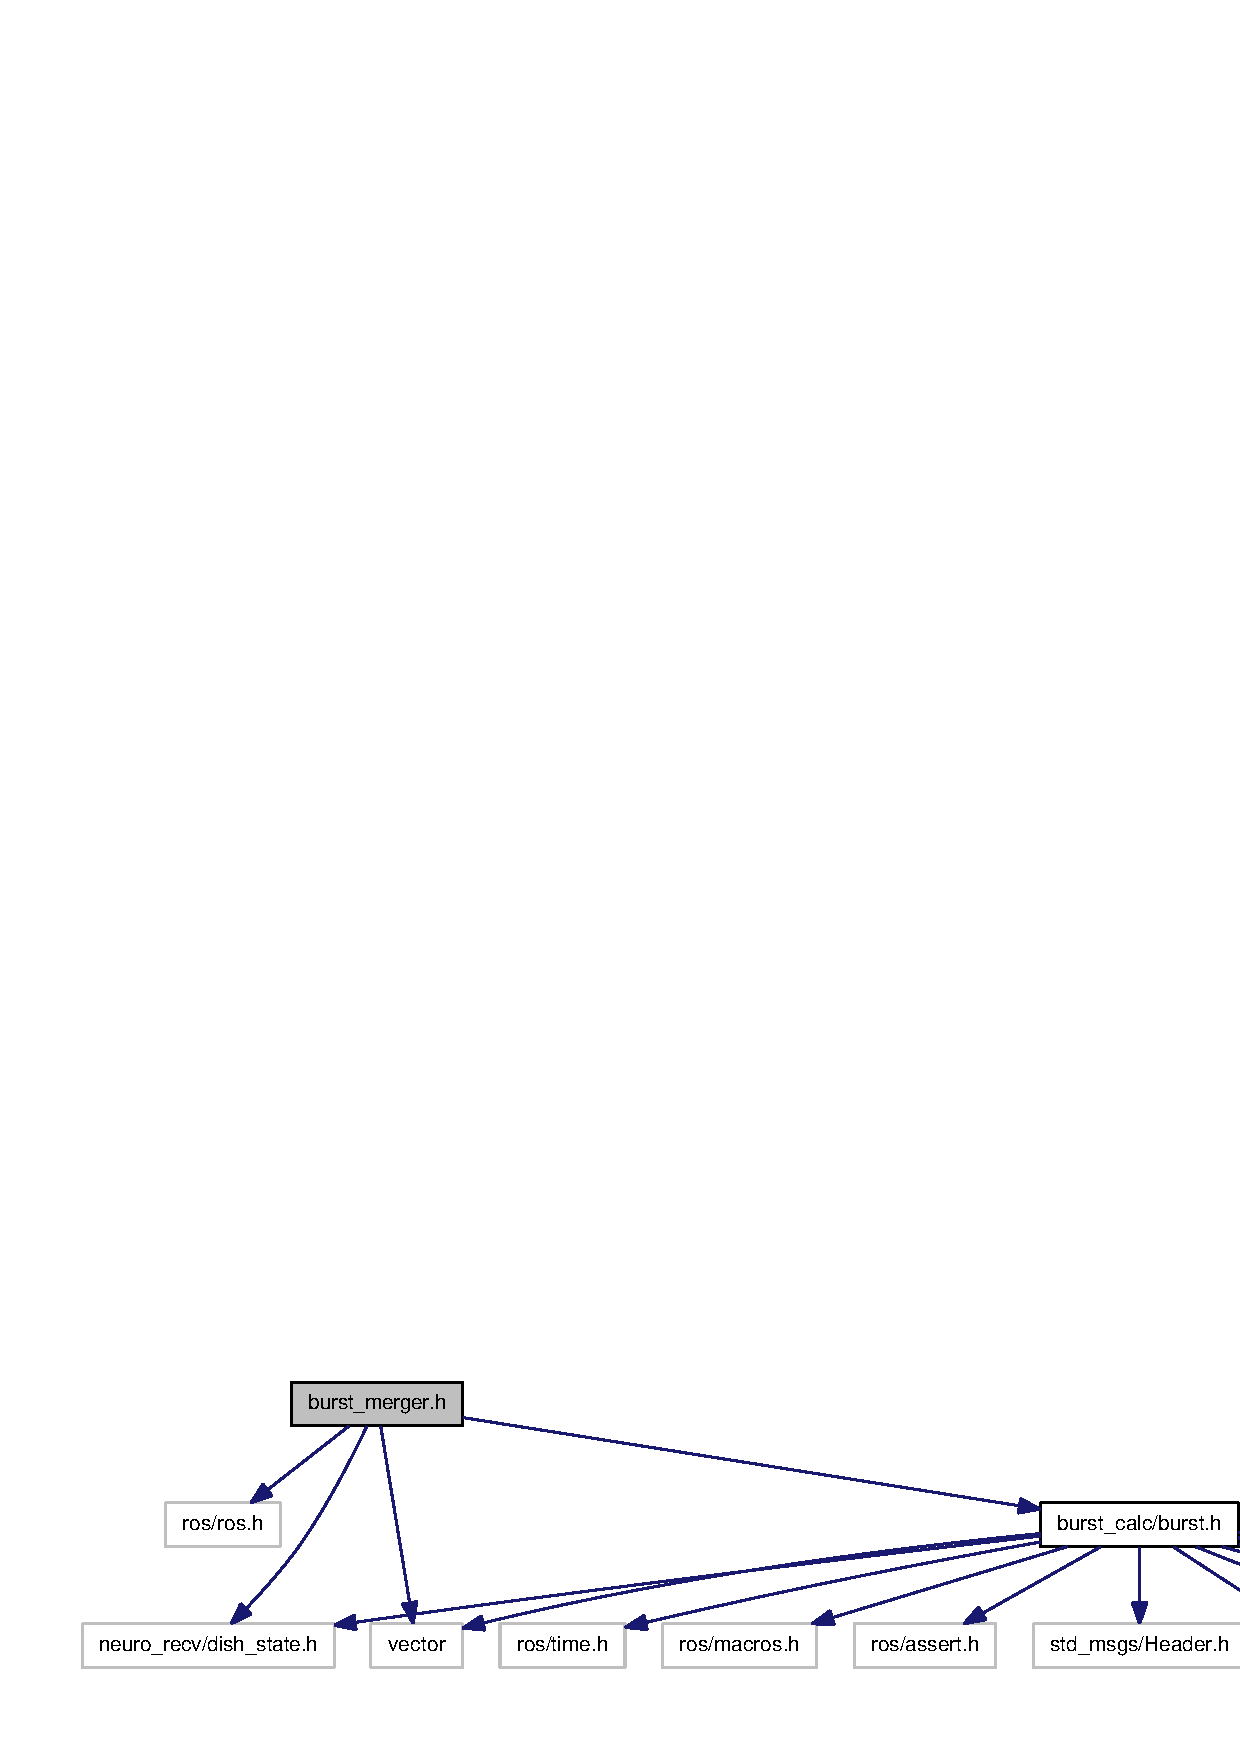
\includegraphics[width=350pt]{burst__merger_8h__incl}
\end{center}
\end{figure}
\-This graph shows which files directly or indirectly include this file\-:\nopagebreak
\begin{figure}[H]
\begin{center}
\leavevmode
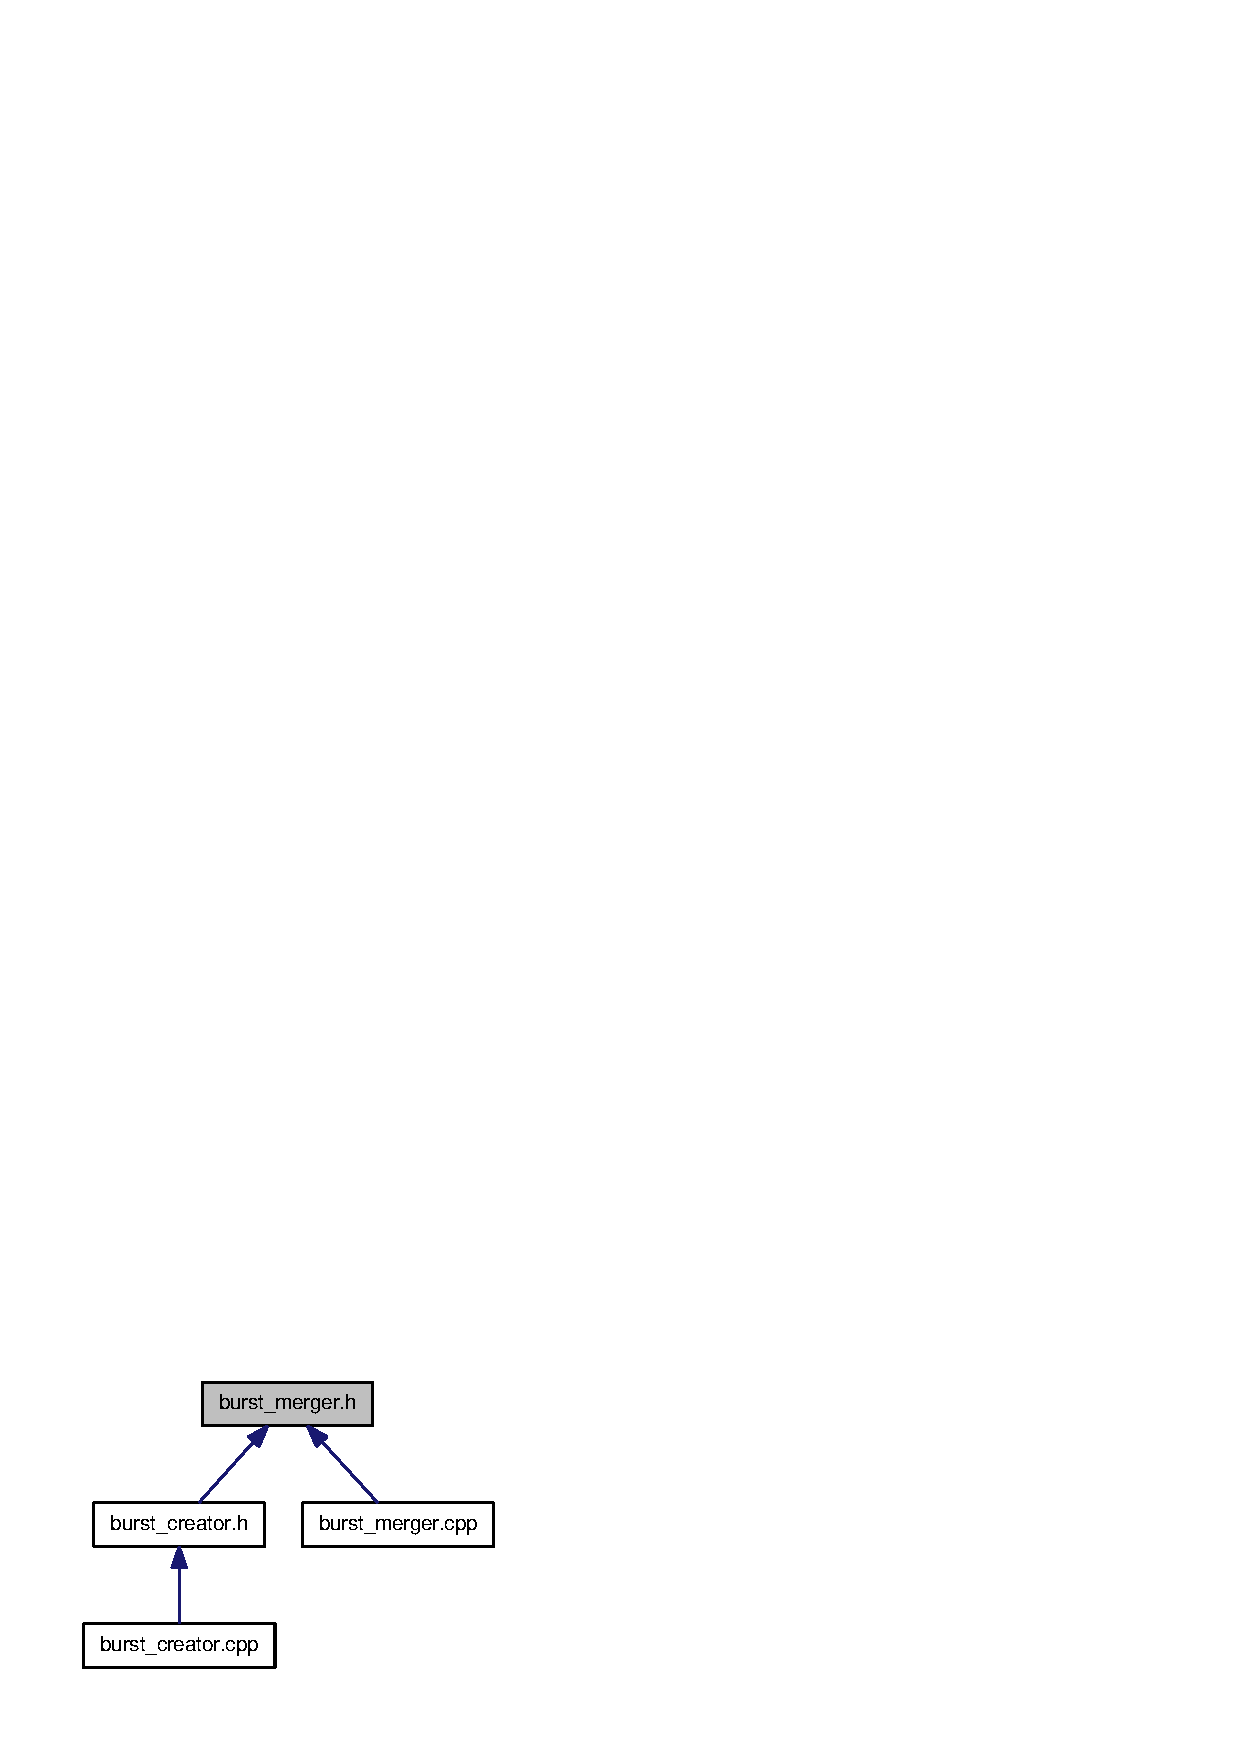
\includegraphics[width=241pt]{burst__merger_8h__dep__incl}
\end{center}
\end{figure}
\subsection*{\-Classes}
\begin{DoxyCompactItemize}
\item 
class {\bf \-Burst\-Merger}
\begin{DoxyCompactList}\small\item\em \-Helper class for the burst\-\_\-creator node. \end{DoxyCompactList}\end{DoxyCompactItemize}

\section{ca.\-h \-File \-Reference}
\label{ca_8h}\index{ca.\-h@{ca.\-h}}
{\ttfamily \#include $<$string$>$}\*
{\ttfamily \#include $<$vector$>$}\*
{\ttfamily \#include $<$map$>$}\*
{\ttfamily \#include $<$ostream$>$}\*
{\ttfamily \#include \char`\"{}ros/serialization.\-h\char`\"{}}\*
{\ttfamily \#include \char`\"{}ros/builtin\-\_\-message\-\_\-traits.\-h\char`\"{}}\*
{\ttfamily \#include \char`\"{}ros/message\-\_\-operations.\-h\char`\"{}}\*
{\ttfamily \#include \char`\"{}ros/time.\-h\char`\"{}}\*
{\ttfamily \#include \char`\"{}ros/macros.\-h\char`\"{}}\*
{\ttfamily \#include \char`\"{}ros/assert.\-h\char`\"{}}\*
{\ttfamily \#include \char`\"{}std\-\_\-msgs/\-Header.\-h\char`\"{}}\*
\-Include dependency graph for ca.\-h\-:\nopagebreak
\begin{figure}[H]
\begin{center}
\leavevmode
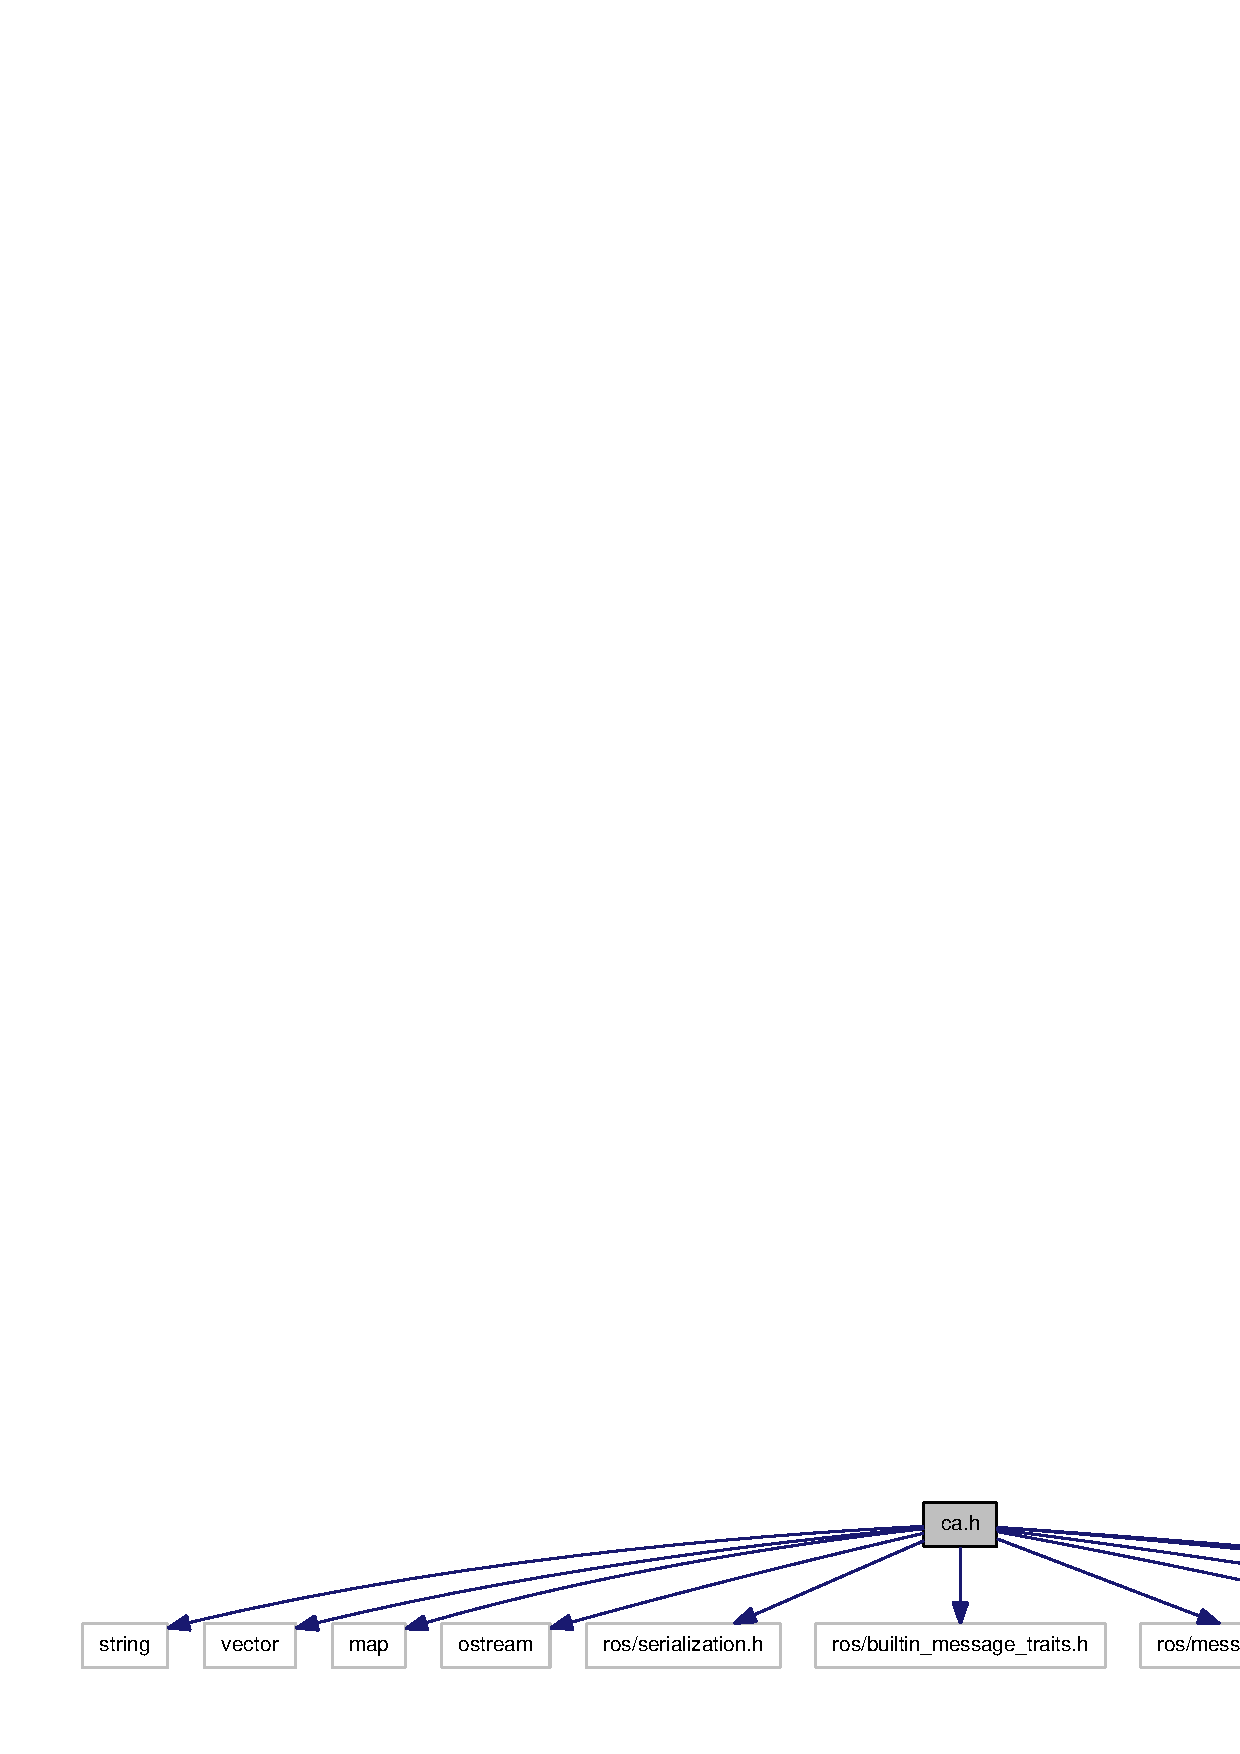
\includegraphics[width=350pt]{ca_8h__incl}
\end{center}
\end{figure}
\-This graph shows which files directly or indirectly include this file\-:\nopagebreak
\begin{figure}[H]
\begin{center}
\leavevmode
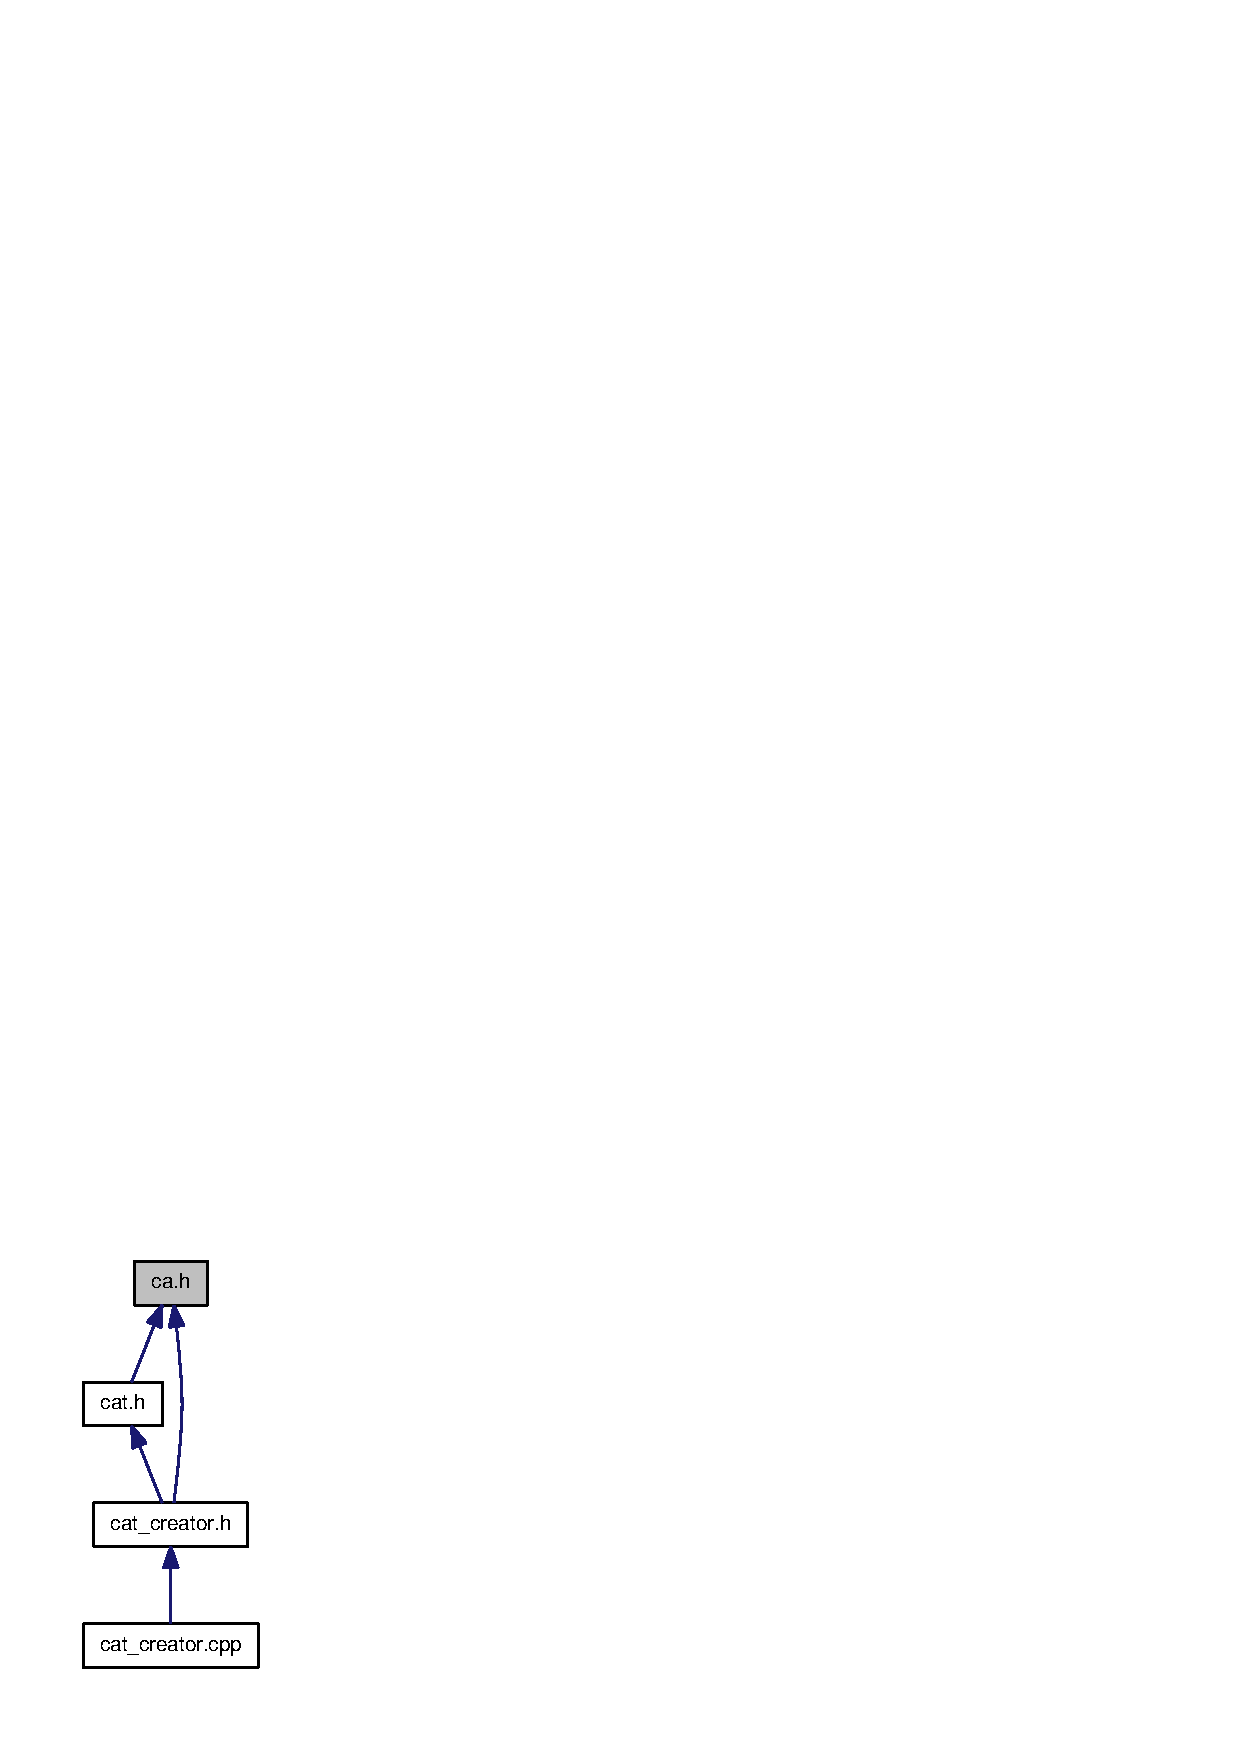
\includegraphics[width=128pt]{ca_8h__dep__incl}
\end{center}
\end{figure}
\subsection*{\-Classes}
\begin{DoxyCompactItemize}
\item 
struct {\bf burst\-\_\-calc\-::ca\-\_\-$<$ Container\-Allocator $>$}
\item 
struct {\bf ros\-::message\-\_\-traits\-::\-Data\-Type$<$ \-::burst\-\_\-calc\-::ca\-\_\-$<$ Container\-Allocator $>$ $>$}
\item 
struct {\bf ros\-::message\-\_\-traits\-::\-Definition$<$ \-::burst\-\_\-calc\-::ca\-\_\-$<$ Container\-Allocator $>$ $>$}
\item 
struct {\bf ros\-::message\-\_\-traits\-::\-Has\-Header$<$ \-::burst\-\_\-calc\-::ca\-\_\-$<$ Container\-Allocator $>$ $>$}
\item 
struct {\bf ros\-::message\-\_\-traits\-::\-Has\-Header$<$ const \-::burst\-\_\-calc\-::ca\-\_\-$<$ Container\-Allocator $>$ $>$}
\item 
struct {\bf ros\-::message\-\_\-traits\-::\-Is\-Message$<$ \-::burst\-\_\-calc\-::ca\-\_\-$<$ Container\-Allocator $>$ $>$}
\item 
struct {\bf ros\-::message\-\_\-traits\-::\-Is\-Message$<$ \-::burst\-\_\-calc\-::ca\-\_\-$<$ Container\-Allocator $>$const  $>$}
\item 
struct {\bf ros\-::message\-\_\-traits\-::\-M\-D5\-Sum$<$ \-::burst\-\_\-calc\-::ca\-\_\-$<$ Container\-Allocator $>$ $>$}
\item 
struct {\bf ros\-::message\-\_\-operations\-::\-Printer$<$ \-::burst\-\_\-calc\-::ca\-\_\-$<$ Container\-Allocator $>$ $>$}
\item 
struct {\bf ros\-::serialization\-::\-Serializer$<$ \-::burst\-\_\-calc\-::ca\-\_\-$<$ Container\-Allocator $>$ $>$}
\end{DoxyCompactItemize}
\subsection*{\-Namespaces}
\begin{DoxyCompactItemize}
\item 
namespace {\bf burst\-\_\-calc}
\item 
namespace {\bf ros}
\item 
namespace {\bf ros\-::message\-\_\-operations}
\item 
namespace {\bf ros\-::message\-\_\-traits}
\item 
namespace {\bf ros\-::serialization}
\end{DoxyCompactItemize}
\subsection*{\-Typedefs}
\begin{DoxyCompactItemize}
\item 
typedef \-::{\bf burst\-\_\-calc\-::ca\-\_\-}\*
$<$ std\-::allocator$<$ void $>$ $>$ {\bf burst\-\_\-calc\-::ca}
\item 
typedef boost\-::shared\-\_\-ptr\*
$<$ \-::{\bf burst\-\_\-calc\-::ca} const  $>$ {\bf burst\-\_\-calc\-::ca\-Const\-Ptr}
\item 
typedef boost\-::shared\-\_\-ptr\*
$<$ \-::{\bf burst\-\_\-calc\-::ca} $>$ {\bf burst\-\_\-calc\-::ca\-Ptr}
\end{DoxyCompactItemize}
\subsection*{\-Functions}
\begin{DoxyCompactItemize}
\item 
{\footnotesize template$<$typename Container\-Allocator $>$ }\\std\-::ostream \& {\bf burst\-\_\-calc\-::operator$<$$<$} (std\-::ostream \&s, const \-::{\bf burst\-\_\-calc\-::ca\-\_\-}$<$ \-Container\-Allocator $>$ \&v)
\end{DoxyCompactItemize}

\section{cat.\-h \-File \-Reference}
\label{cat_8h}\index{cat.\-h@{cat.\-h}}
{\ttfamily \#include $<$string$>$}\*
{\ttfamily \#include $<$vector$>$}\*
{\ttfamily \#include $<$map$>$}\*
{\ttfamily \#include $<$ostream$>$}\*
{\ttfamily \#include \char`\"{}ros/serialization.\-h\char`\"{}}\*
{\ttfamily \#include \char`\"{}ros/builtin\-\_\-message\-\_\-traits.\-h\char`\"{}}\*
{\ttfamily \#include \char`\"{}ros/message\-\_\-operations.\-h\char`\"{}}\*
{\ttfamily \#include \char`\"{}ros/time.\-h\char`\"{}}\*
{\ttfamily \#include \char`\"{}ros/macros.\-h\char`\"{}}\*
{\ttfamily \#include \char`\"{}ros/assert.\-h\char`\"{}}\*
{\ttfamily \#include \char`\"{}std\-\_\-msgs/\-Header.\-h\char`\"{}}\*
{\ttfamily \#include \char`\"{}burst\-\_\-calc/ca.\-h\char`\"{}}\*
\-Include dependency graph for cat.\-h\-:\nopagebreak
\begin{figure}[H]
\begin{center}
\leavevmode
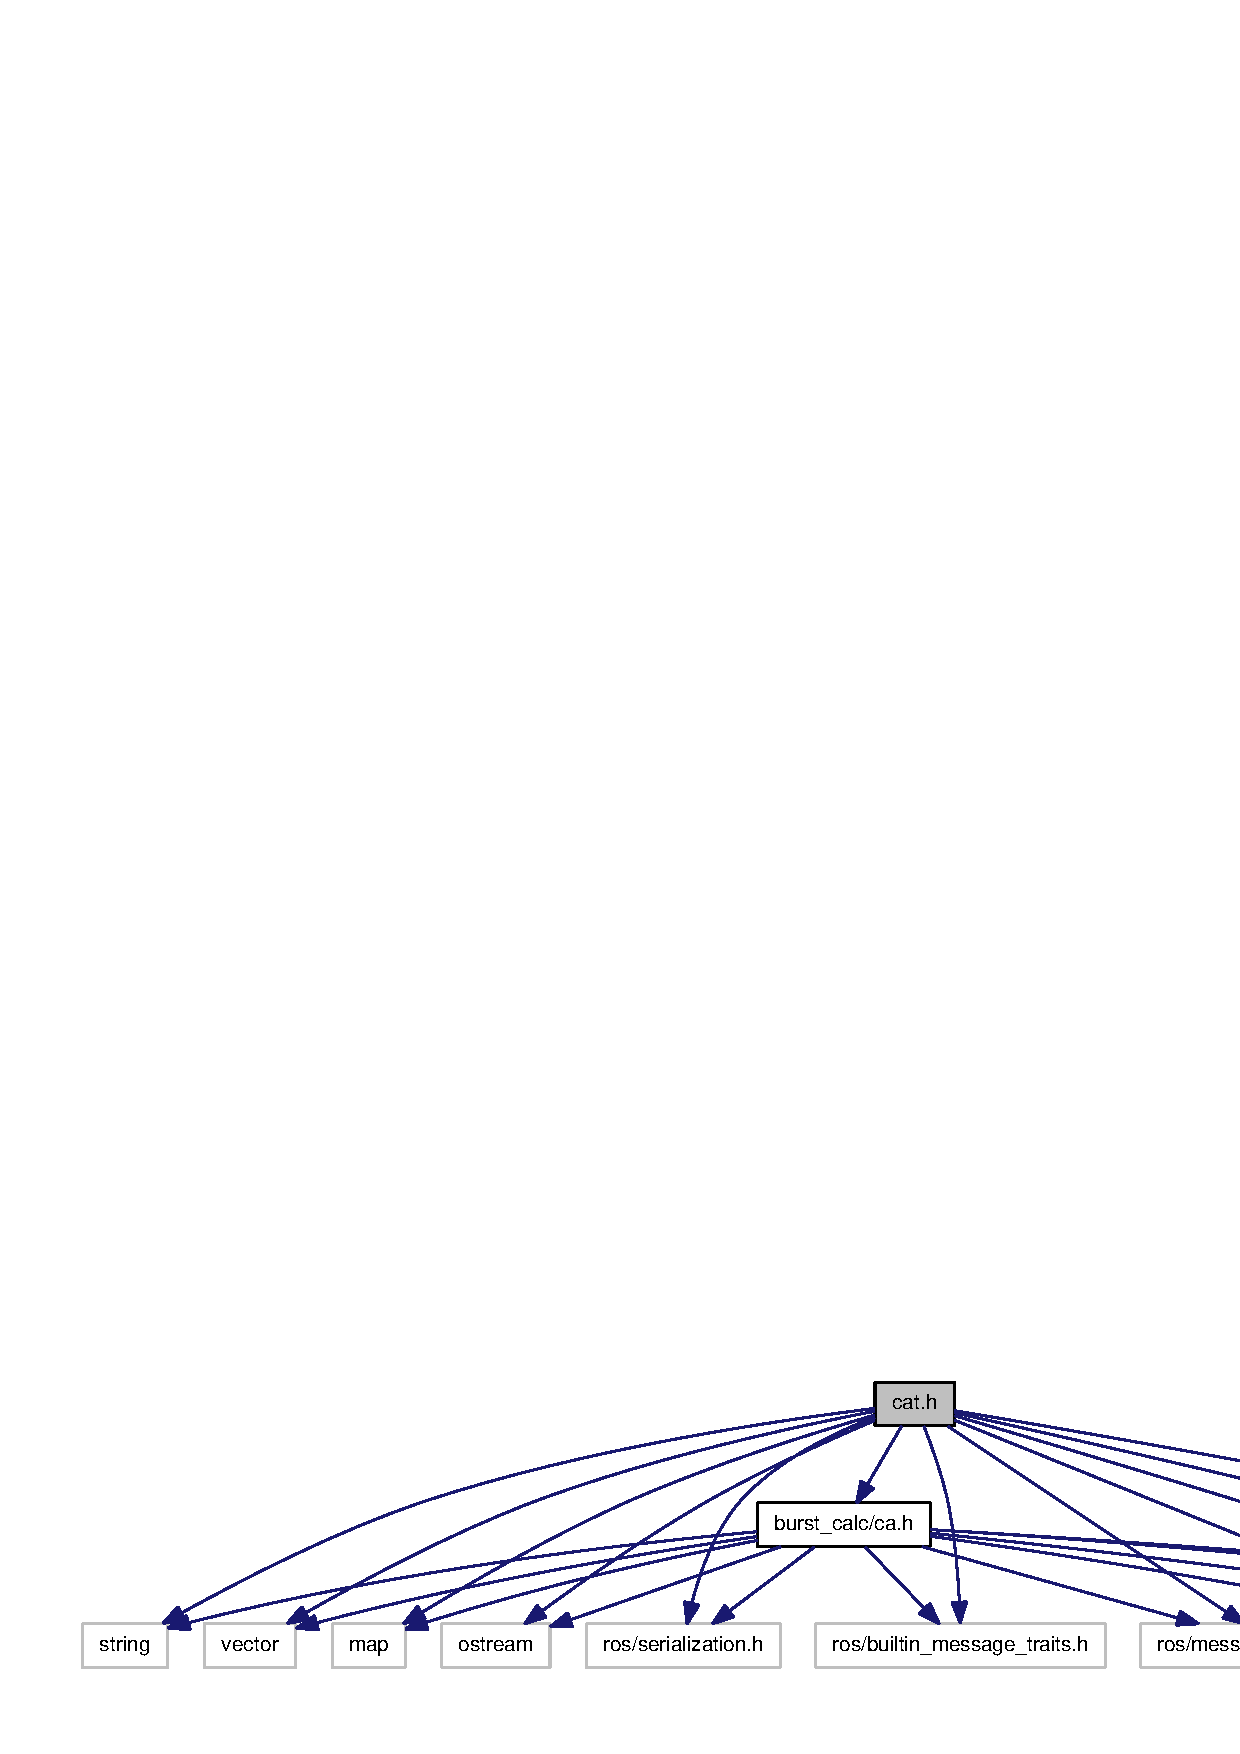
\includegraphics[width=350pt]{cat_8h__incl}
\end{center}
\end{figure}
\-This graph shows which files directly or indirectly include this file\-:\nopagebreak
\begin{figure}[H]
\begin{center}
\leavevmode
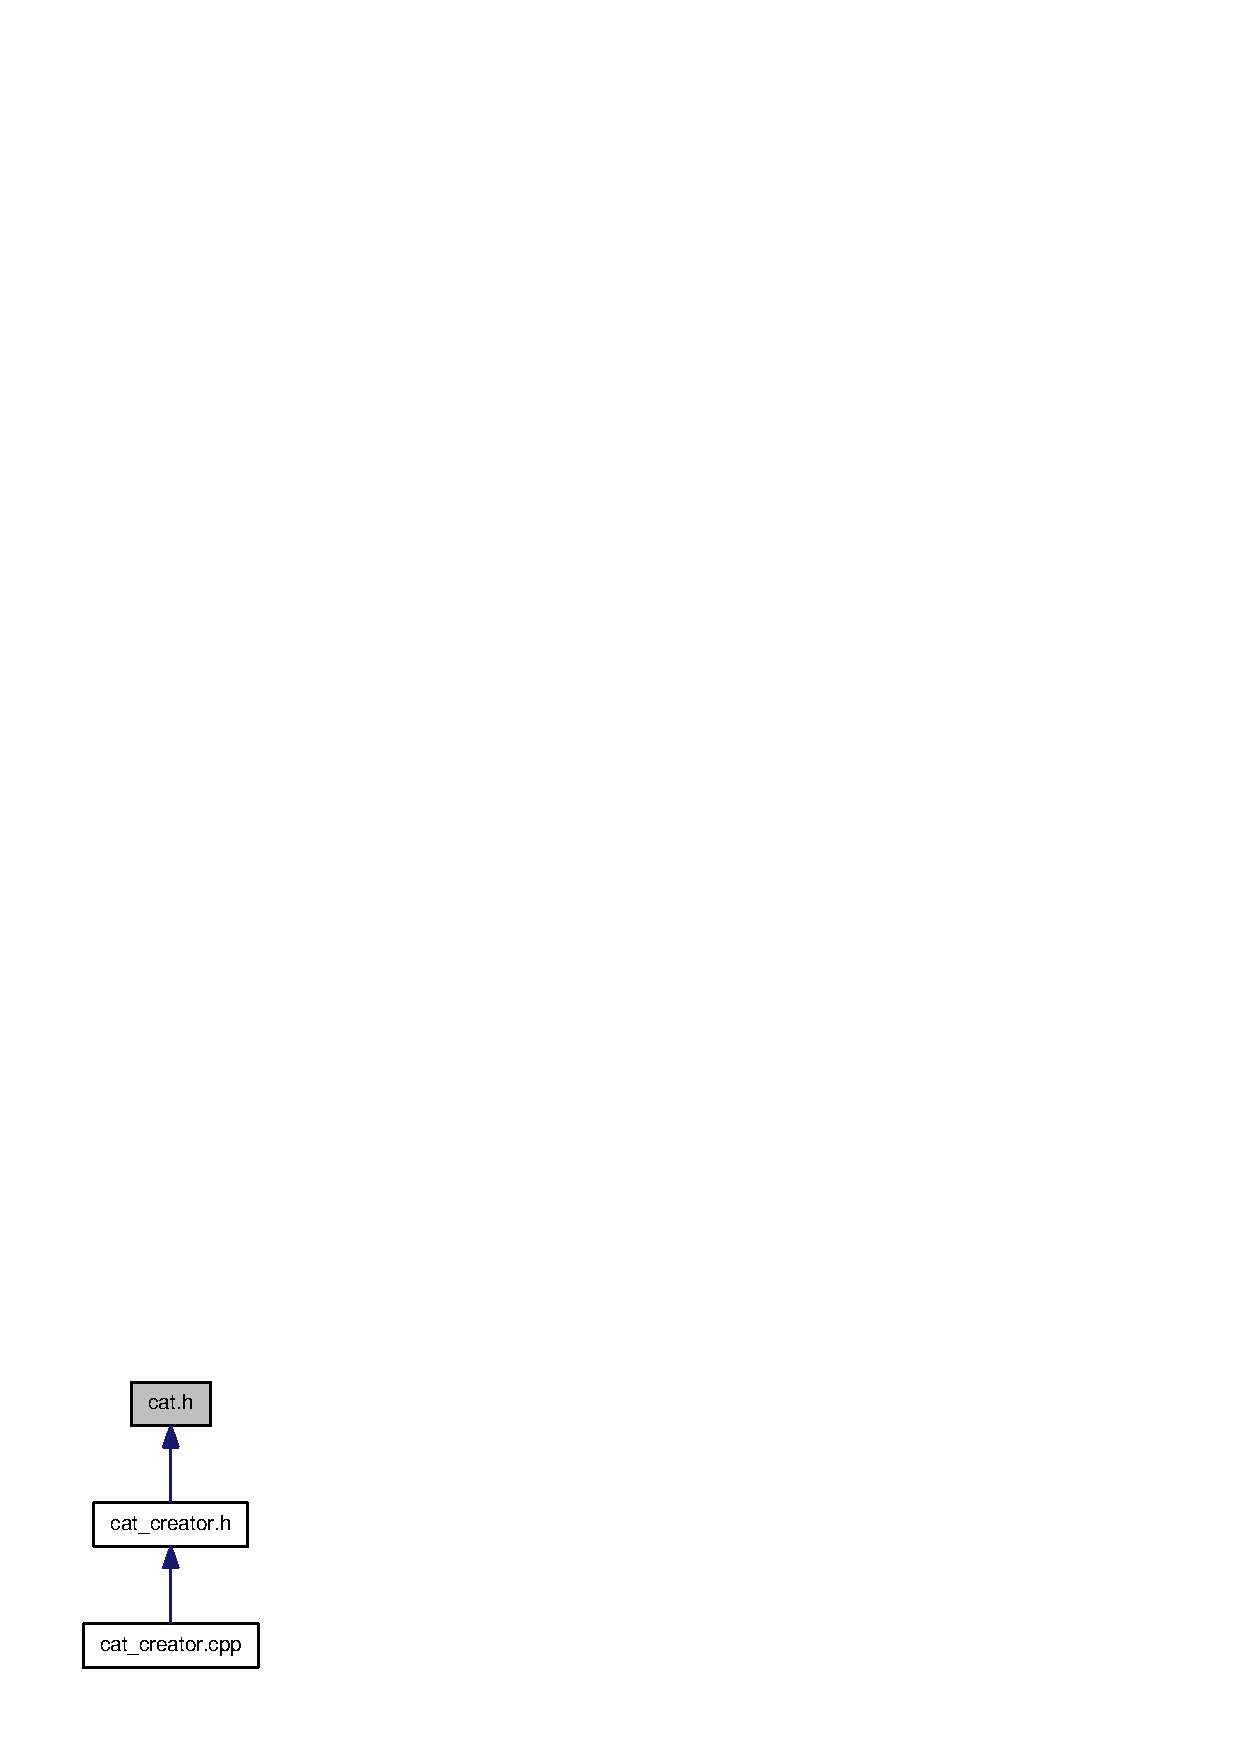
\includegraphics[width=128pt]{cat_8h__dep__incl}
\end{center}
\end{figure}
\subsection*{\-Classes}
\begin{DoxyCompactItemize}
\item 
struct {\bf burst\-\_\-calc\-::cat\-\_\-$<$ Container\-Allocator $>$}
\item 
struct {\bf ros\-::message\-\_\-traits\-::\-Data\-Type$<$ \-::burst\-\_\-calc\-::cat\-\_\-$<$ Container\-Allocator $>$ $>$}
\item 
struct {\bf ros\-::message\-\_\-traits\-::\-Definition$<$ \-::burst\-\_\-calc\-::cat\-\_\-$<$ Container\-Allocator $>$ $>$}
\item 
struct {\bf ros\-::message\-\_\-traits\-::\-Has\-Header$<$ \-::burst\-\_\-calc\-::cat\-\_\-$<$ Container\-Allocator $>$ $>$}
\item 
struct {\bf ros\-::message\-\_\-traits\-::\-Has\-Header$<$ const \-::burst\-\_\-calc\-::cat\-\_\-$<$ Container\-Allocator $>$ $>$}
\item 
struct {\bf ros\-::message\-\_\-traits\-::\-Is\-Message$<$ \-::burst\-\_\-calc\-::cat\-\_\-$<$ Container\-Allocator $>$ $>$}
\item 
struct {\bf ros\-::message\-\_\-traits\-::\-Is\-Message$<$ \-::burst\-\_\-calc\-::cat\-\_\-$<$ Container\-Allocator $>$const  $>$}
\item 
struct {\bf ros\-::message\-\_\-traits\-::\-M\-D5\-Sum$<$ \-::burst\-\_\-calc\-::cat\-\_\-$<$ Container\-Allocator $>$ $>$}
\item 
struct {\bf ros\-::message\-\_\-operations\-::\-Printer$<$ \-::burst\-\_\-calc\-::cat\-\_\-$<$ Container\-Allocator $>$ $>$}
\item 
struct {\bf ros\-::serialization\-::\-Serializer$<$ \-::burst\-\_\-calc\-::cat\-\_\-$<$ Container\-Allocator $>$ $>$}
\end{DoxyCompactItemize}
\subsection*{\-Namespaces}
\begin{DoxyCompactItemize}
\item 
namespace {\bf burst\-\_\-calc}
\item 
namespace {\bf ros}
\item 
namespace {\bf ros\-::message\-\_\-operations}
\item 
namespace {\bf ros\-::message\-\_\-traits}
\item 
namespace {\bf ros\-::serialization}
\end{DoxyCompactItemize}
\subsection*{\-Typedefs}
\begin{DoxyCompactItemize}
\item 
typedef \-::{\bf burst\-\_\-calc\-::cat\-\_\-}\*
$<$ std\-::allocator$<$ void $>$ $>$ {\bf burst\-\_\-calc\-::cat}
\item 
typedef boost\-::shared\-\_\-ptr\*
$<$ \-::{\bf burst\-\_\-calc\-::cat} const  $>$ {\bf burst\-\_\-calc\-::cat\-Const\-Ptr}
\item 
typedef boost\-::shared\-\_\-ptr\*
$<$ \-::{\bf burst\-\_\-calc\-::cat} $>$ {\bf burst\-\_\-calc\-::cat\-Ptr}
\end{DoxyCompactItemize}
\subsection*{\-Functions}
\begin{DoxyCompactItemize}
\item 
{\footnotesize template$<$typename Container\-Allocator $>$ }\\std\-::ostream \& {\bf burst\-\_\-calc\-::operator$<$$<$} (std\-::ostream \&s, const \-::{\bf burst\-\_\-calc\-::cat\-\_\-}$<$ \-Container\-Allocator $>$ \&v)
\end{DoxyCompactItemize}

\section{cat\-\_\-creator.\-cpp \-File \-Reference}
\label{cat__creator_8cpp}\index{cat\-\_\-creator.\-cpp@{cat\-\_\-creator.\-cpp}}
{\ttfamily \#include \char`\"{}burst\-\_\-calc/cat\-\_\-creator.\-h\char`\"{}}\*
{\ttfamily \#include $<$cstdio$>$}\*
\-Include dependency graph for cat\-\_\-creator.\-cpp\-:\nopagebreak
\begin{figure}[H]
\begin{center}
\leavevmode
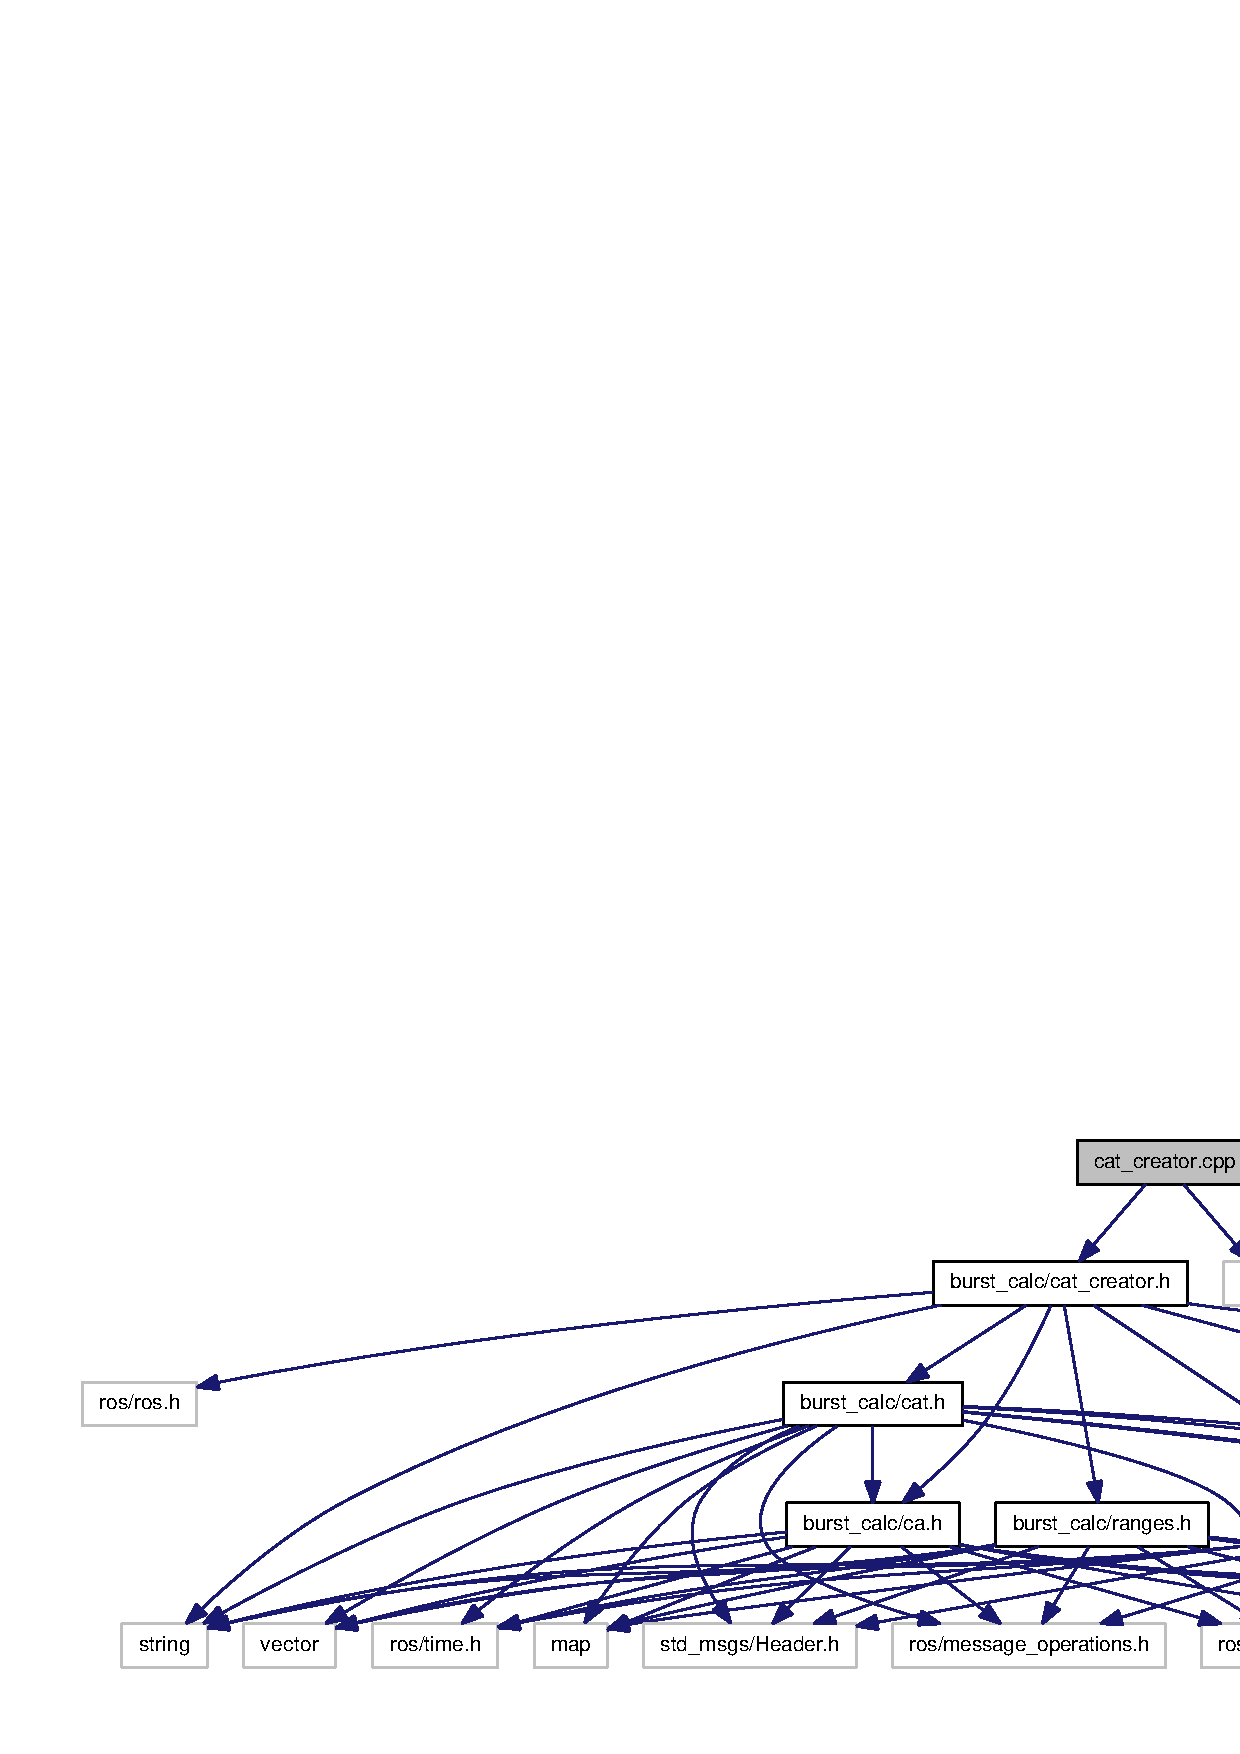
\includegraphics[width=350pt]{cat__creator_8cpp__incl}
\end{center}
\end{figure}
\subsection*{\-Functions}
\begin{DoxyCompactItemize}
\item 
int {\bf main} (int argc, char $\ast$$\ast$argv)
\begin{DoxyCompactList}\small\item\em \-Creates an instance of the node. \end{DoxyCompactList}\end{DoxyCompactItemize}


\subsection{\-Function \-Documentation}
\index{cat\-\_\-creator.\-cpp@{cat\-\_\-creator.\-cpp}!main@{main}}
\index{main@{main}!cat_creator.cpp@{cat\-\_\-creator.\-cpp}}
\subsubsection[{main}]{\setlength{\rightskip}{0pt plus 5cm}int {\bf main} (
\begin{DoxyParamCaption}
\item[{int}]{argc, }
\item[{char $\ast$$\ast$}]{argv}
\end{DoxyParamCaption}
)}\label{cat__creator_8cpp_a3c04138a5bfe5d72780bb7e82a18e627}


\-Creates an instance of the node. 



\-Definition at line 311 of file cat\-\_\-creator.\-cpp.


\section{cat\-\_\-creator.\-h \-File \-Reference}
\label{cat__creator_8h}\index{cat\-\_\-creator.\-h@{cat\-\_\-creator.\-h}}
{\ttfamily \#include \char`\"{}ros/ros.\-h\char`\"{}}\*
{\ttfamily \#include \char`\"{}burst\-\_\-calc/burst.\-h\char`\"{}}\*
{\ttfamily \#include \char`\"{}burst\-\_\-calc/ranges.\-h\char`\"{}}\*
{\ttfamily \#include \char`\"{}burst\-\_\-calc/cat.\-h\char`\"{}}\*
{\ttfamily \#include \char`\"{}burst\-\_\-calc/ca.\-h\char`\"{}}\*
{\ttfamily \#include \char`\"{}neuro\-\_\-recv/dish\-\_\-state.\-h\char`\"{}}\*
{\ttfamily \#include $<$fstream$>$}\*
{\ttfamily \#include $<$string$>$}\*
\-Include dependency graph for cat\-\_\-creator.\-h\-:\nopagebreak
\begin{figure}[H]
\begin{center}
\leavevmode
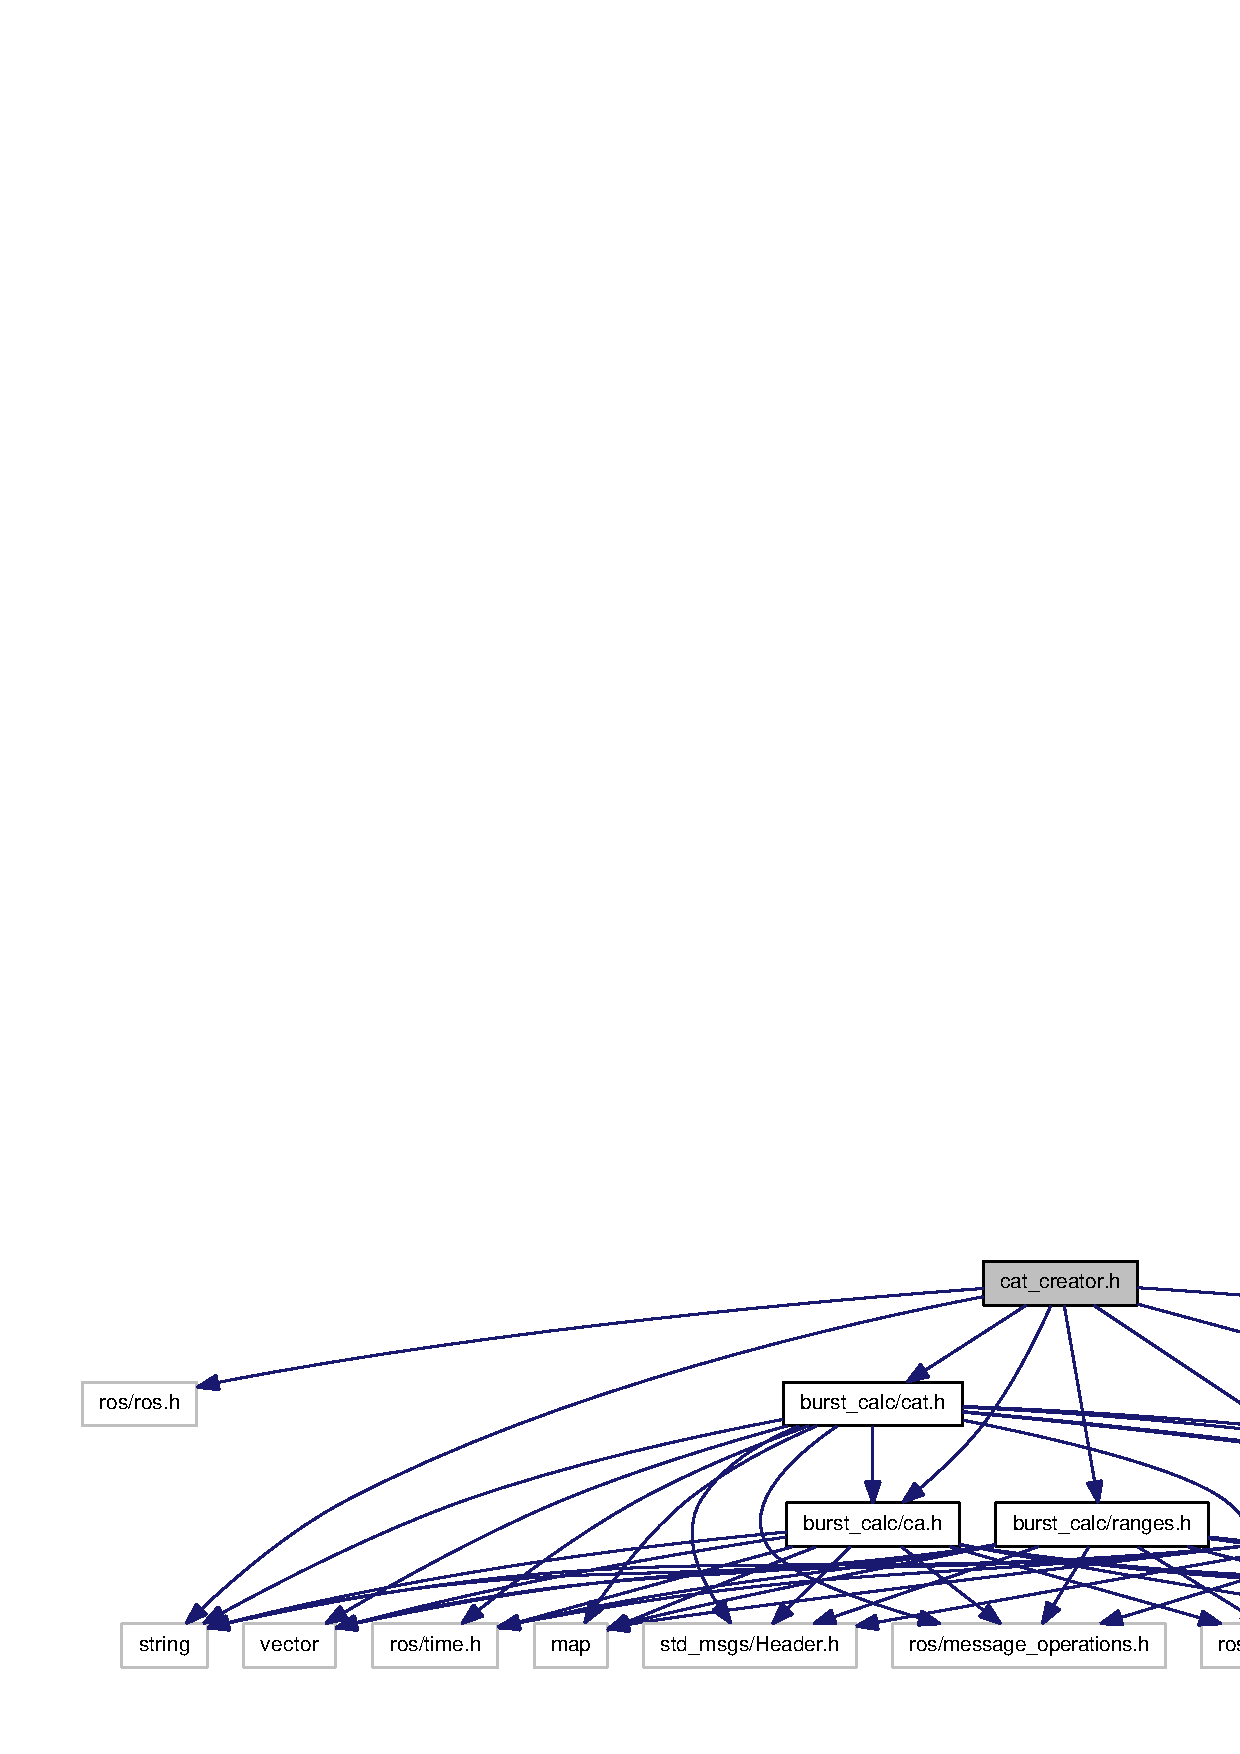
\includegraphics[width=350pt]{cat__creator_8h__incl}
\end{center}
\end{figure}
\-This graph shows which files directly or indirectly include this file\-:\nopagebreak
\begin{figure}[H]
\begin{center}
\leavevmode
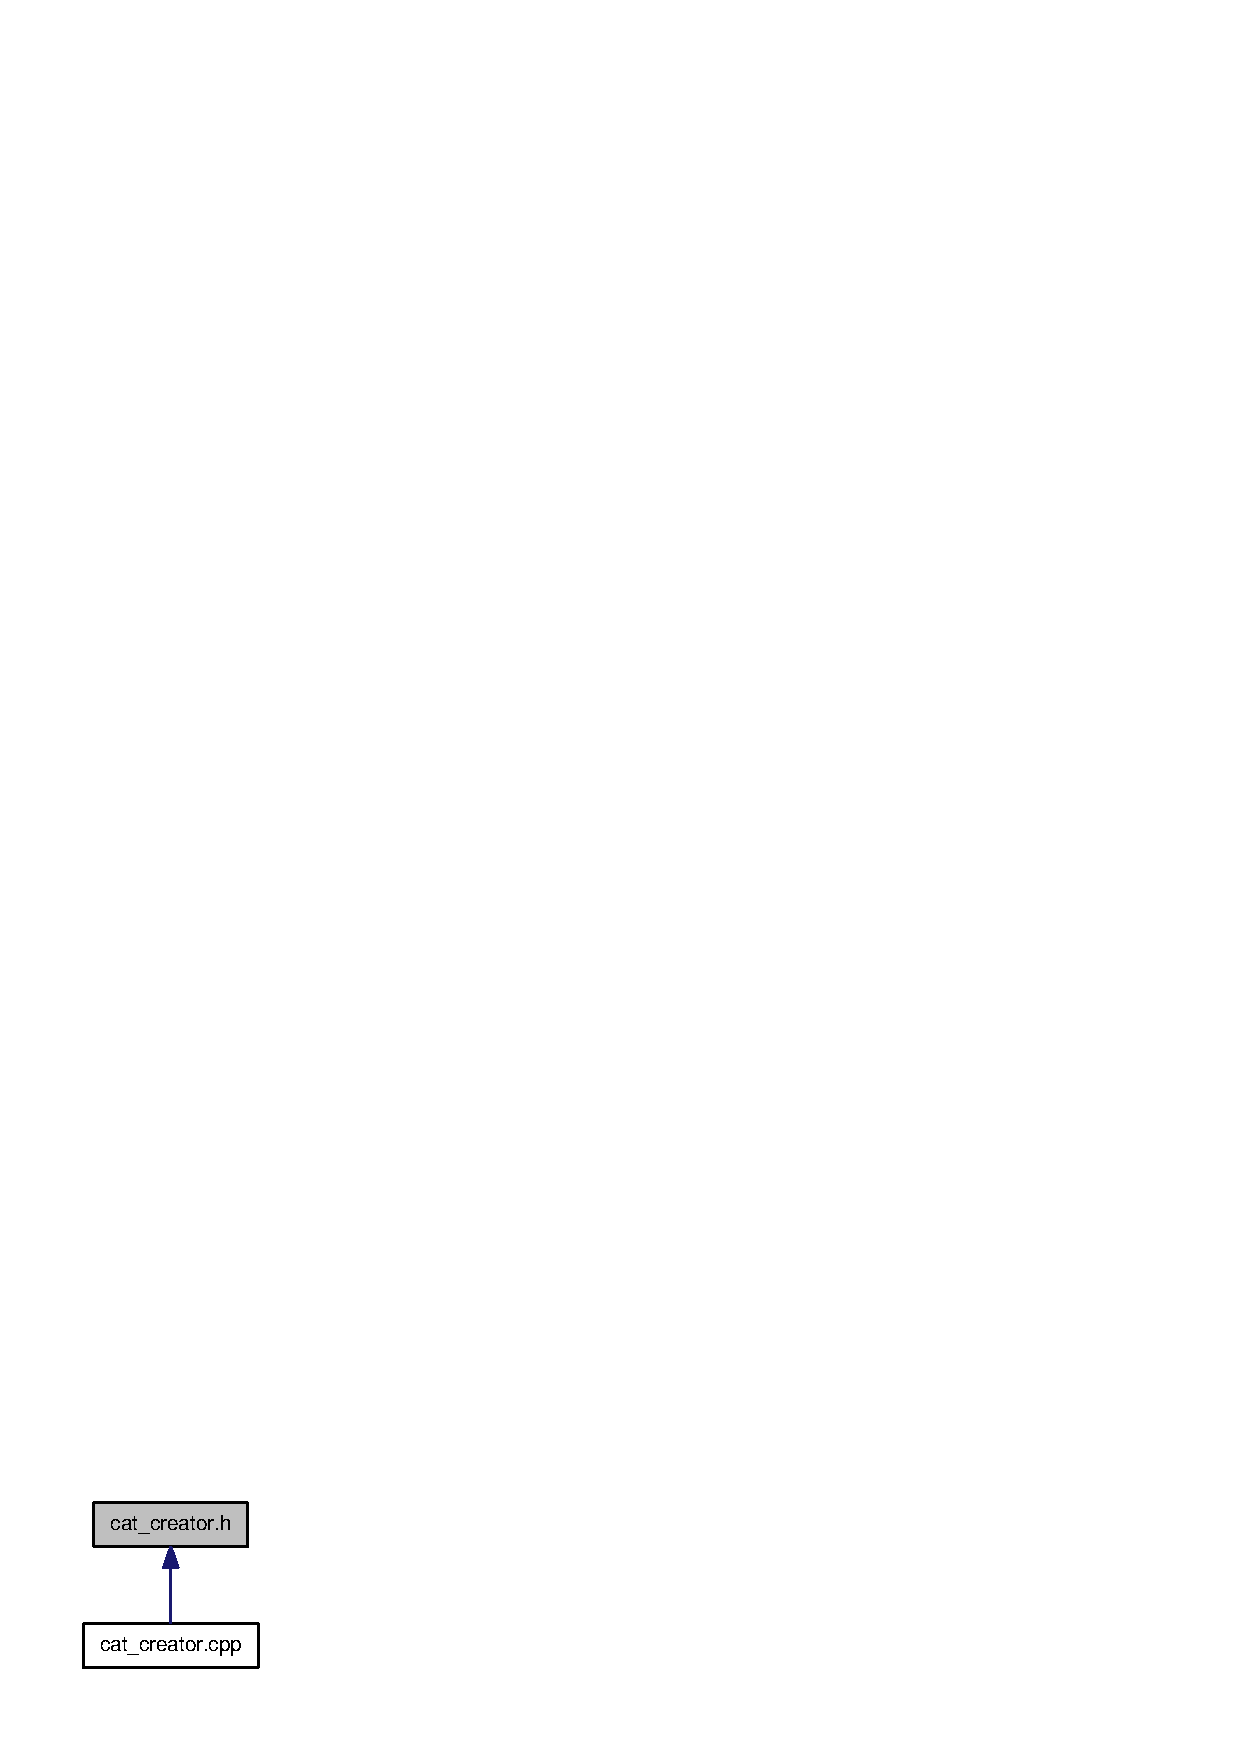
\includegraphics[width=128pt]{cat__creator_8h__dep__incl}
\end{center}
\end{figure}
\subsection*{\-Classes}
\begin{DoxyCompactItemize}
\item 
class {\bf \-Cat\-Creator}
\begin{DoxyCompactList}\small\item\em \-Node for creating \-C\-A\-Ts (center of activity trajectories) \end{DoxyCompactList}\end{DoxyCompactItemize}
\subsection*{\-Variables}
\begin{DoxyCompactItemize}
\item 
const int {\bf \-X\-\_\-\-C\-O\-O\-R\-D\-\_\-} [60]
\item 
const int {\bf \-Y\-\_\-\-C\-O\-O\-R\-D\-\_\-} [60]
\end{DoxyCompactItemize}


\subsection{\-Variable \-Documentation}
\index{cat\-\_\-creator.\-h@{cat\-\_\-creator.\-h}!\-X\-\_\-\-C\-O\-O\-R\-D\-\_\-@{\-X\-\_\-\-C\-O\-O\-R\-D\-\_\-}}
\index{\-X\-\_\-\-C\-O\-O\-R\-D\-\_\-@{\-X\-\_\-\-C\-O\-O\-R\-D\-\_\-}!cat_creator.h@{cat\-\_\-creator.\-h}}
\subsubsection[{\-X\-\_\-\-C\-O\-O\-R\-D\-\_\-}]{\setlength{\rightskip}{0pt plus 5cm}const int {\bf \-X\-\_\-\-C\-O\-O\-R\-D\-\_\-}[60]}\label{cat__creator_8h_ab5f3225d11c3b94b559538383626bc05}
{\bfseries \-Initial value\-:}
\begin{DoxyCode}
 {    2, 3, 4, 5, 6, 7,
                           1, 2, 3, 4, 5, 6, 7, 8,
                           1, 2, 3, 4, 5, 6, 7, 8,
                           1, 2, 3, 4, 5, 6, 7, 8,
                           1, 2, 3, 4, 5, 6, 7, 8,
                           1, 2, 3, 4, 5, 6, 7, 8,
                           1, 2, 3, 4, 5, 6, 7, 8,
                              2, 3, 4, 5, 6, 7     }
\end{DoxyCode}


\-Definition at line 19 of file cat\-\_\-creator.\-h.

\index{cat\-\_\-creator.\-h@{cat\-\_\-creator.\-h}!\-Y\-\_\-\-C\-O\-O\-R\-D\-\_\-@{\-Y\-\_\-\-C\-O\-O\-R\-D\-\_\-}}
\index{\-Y\-\_\-\-C\-O\-O\-R\-D\-\_\-@{\-Y\-\_\-\-C\-O\-O\-R\-D\-\_\-}!cat_creator.h@{cat\-\_\-creator.\-h}}
\subsubsection[{\-Y\-\_\-\-C\-O\-O\-R\-D\-\_\-}]{\setlength{\rightskip}{0pt plus 5cm}const int {\bf \-Y\-\_\-\-C\-O\-O\-R\-D\-\_\-}[60]}\label{cat__creator_8h_ad4453466899bf6e878072903395b2a1d}
{\bfseries \-Initial value\-:}
\begin{DoxyCode}
 {    1, 1, 1, 1, 1, 1,
                           2, 2, 2, 2, 2, 2, 2, 2,
                           3, 3, 3, 3, 3, 3, 3, 3,
                           4, 4, 4, 4, 4, 4, 4, 4,
                           5, 5, 5, 5, 5, 5, 5, 5,
                           6, 6, 6, 6, 6, 6, 6, 6,
                           7, 7, 7, 7, 7, 7, 7, 7,
                              8, 8, 8, 8, 8, 8    }
\end{DoxyCode}


\-Definition at line 27 of file cat\-\_\-creator.\-h.


\section{mainpage.\-dox \-File \-Reference}
\label{mainpage_8dox}\index{mainpage.\-dox@{mainpage.\-dox}}

\section{ranges.\-h \-File \-Reference}
\label{ranges_8h}\index{ranges.\-h@{ranges.\-h}}
{\ttfamily \#include $<$string$>$}\*
{\ttfamily \#include $<$vector$>$}\*
{\ttfamily \#include $<$map$>$}\*
{\ttfamily \#include $<$ostream$>$}\*
{\ttfamily \#include \char`\"{}ros/serialization.\-h\char`\"{}}\*
{\ttfamily \#include \char`\"{}ros/builtin\-\_\-message\-\_\-traits.\-h\char`\"{}}\*
{\ttfamily \#include \char`\"{}ros/message\-\_\-operations.\-h\char`\"{}}\*
{\ttfamily \#include \char`\"{}ros/time.\-h\char`\"{}}\*
{\ttfamily \#include \char`\"{}ros/macros.\-h\char`\"{}}\*
{\ttfamily \#include \char`\"{}ros/assert.\-h\char`\"{}}\*
{\ttfamily \#include \char`\"{}std\-\_\-msgs/\-Header.\-h\char`\"{}}\*
\-Include dependency graph for ranges.\-h\-:\nopagebreak
\begin{figure}[H]
\begin{center}
\leavevmode
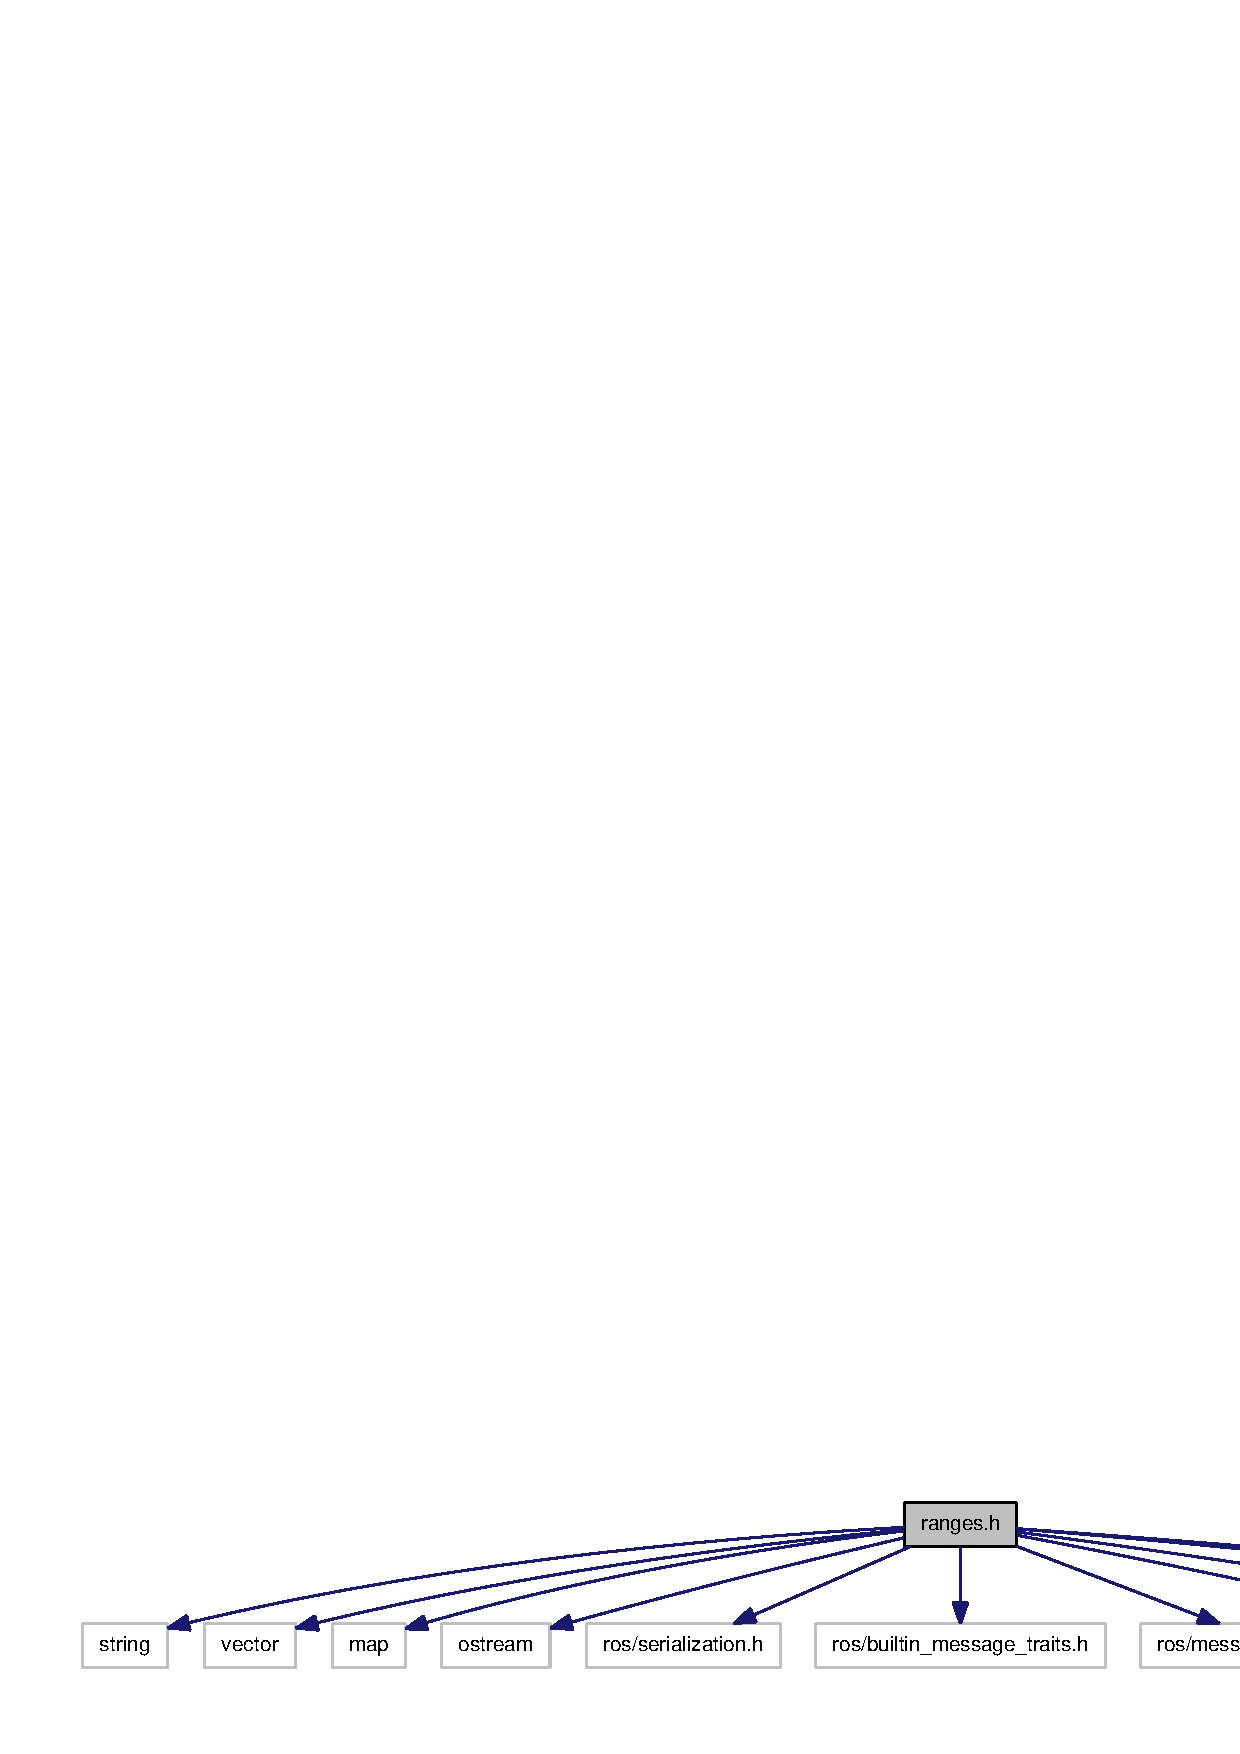
\includegraphics[width=350pt]{ranges_8h__incl}
\end{center}
\end{figure}
\-This graph shows which files directly or indirectly include this file\-:\nopagebreak
\begin{figure}[H]
\begin{center}
\leavevmode
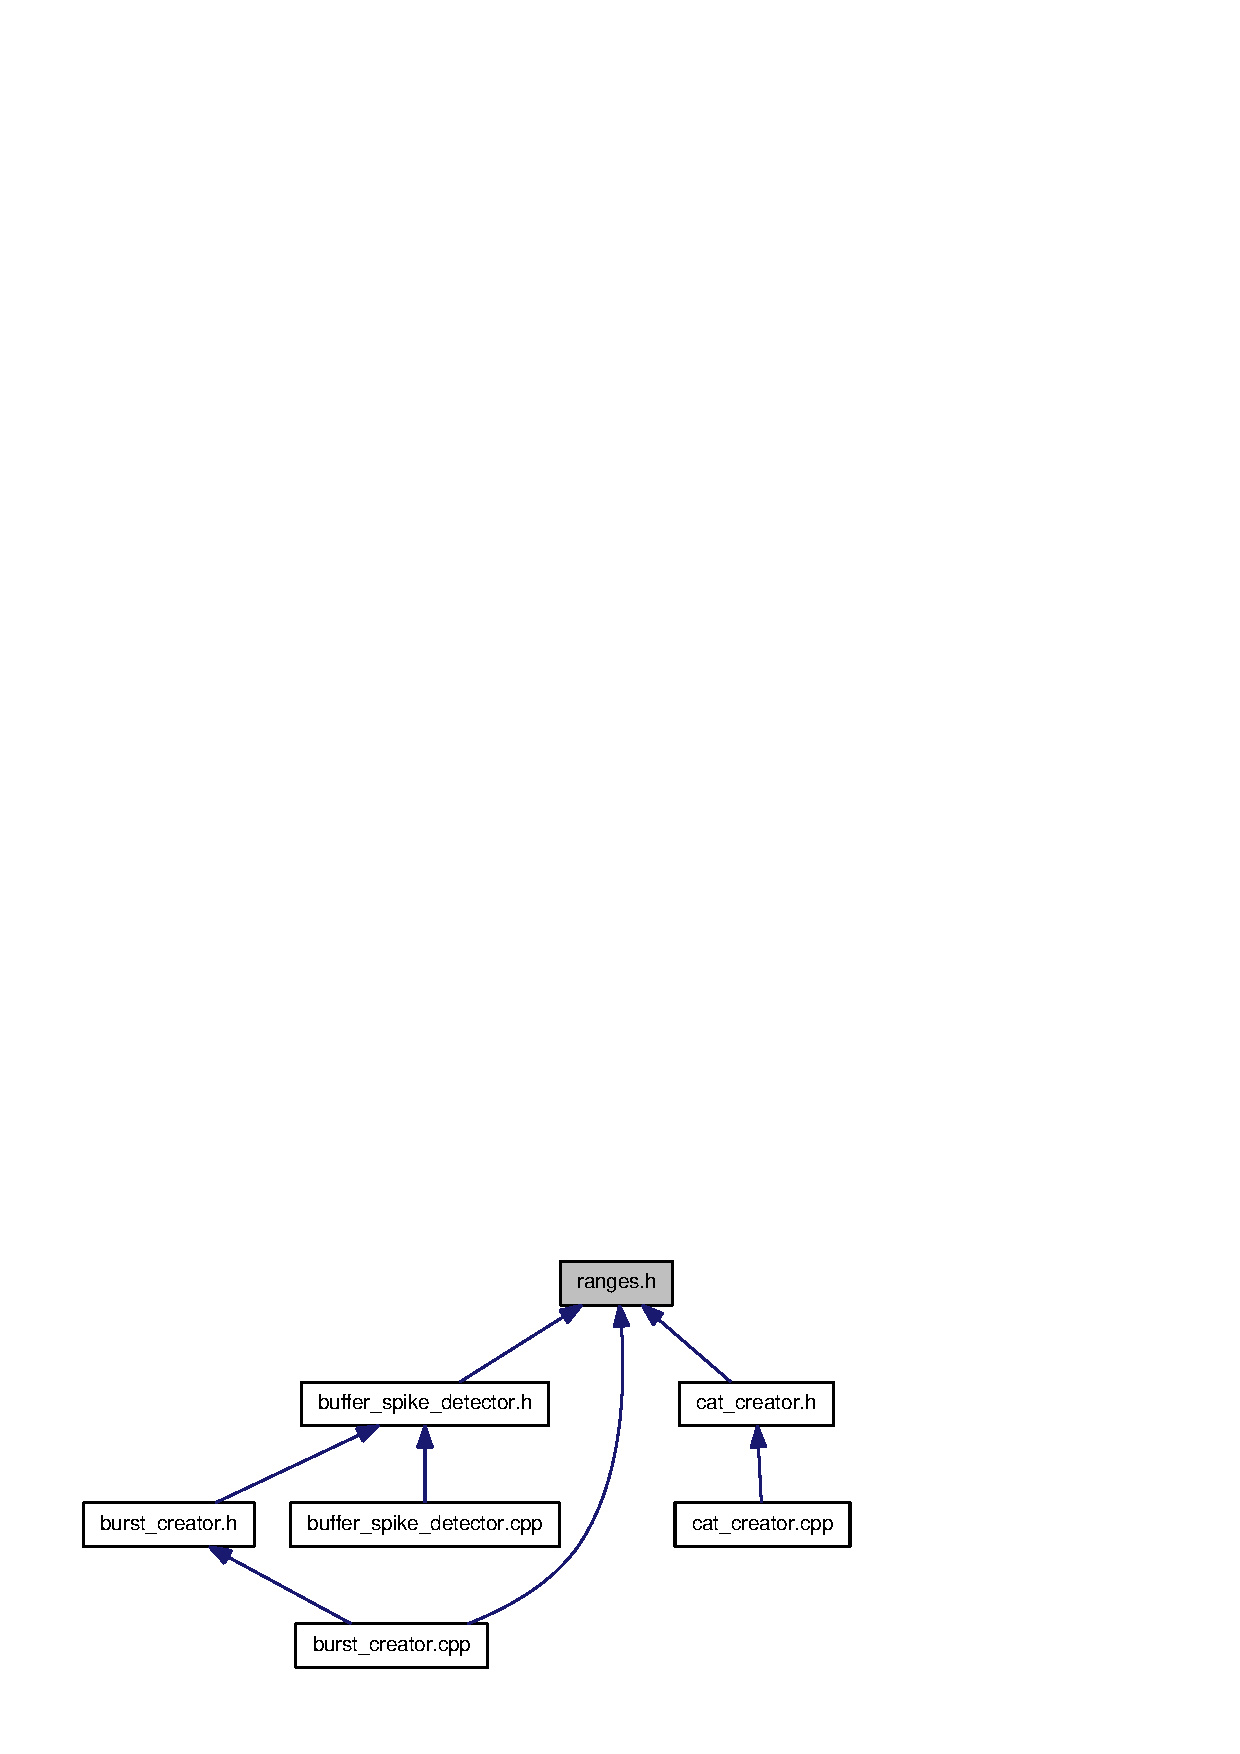
\includegraphics[width=350pt]{ranges_8h__dep__incl}
\end{center}
\end{figure}
\subsection*{\-Classes}
\begin{DoxyCompactItemize}
\item 
struct {\bf ros\-::message\-\_\-traits\-::\-Data\-Type$<$ \-::burst\-\_\-calc\-::ranges\-\_\-$<$ Container\-Allocator $>$ $>$}
\item 
struct {\bf ros\-::message\-\_\-traits\-::\-Definition$<$ \-::burst\-\_\-calc\-::ranges\-\_\-$<$ Container\-Allocator $>$ $>$}
\item 
struct {\bf ros\-::message\-\_\-traits\-::\-Has\-Header$<$ \-::burst\-\_\-calc\-::ranges\-\_\-$<$ Container\-Allocator $>$ $>$}
\item 
struct {\bf ros\-::message\-\_\-traits\-::\-Has\-Header$<$ const \-::burst\-\_\-calc\-::ranges\-\_\-$<$ Container\-Allocator $>$ $>$}
\item 
struct {\bf ros\-::message\-\_\-traits\-::\-Is\-Message$<$ \-::burst\-\_\-calc\-::ranges\-\_\-$<$ Container\-Allocator $>$ $>$}
\item 
struct {\bf ros\-::message\-\_\-traits\-::\-Is\-Message$<$ \-::burst\-\_\-calc\-::ranges\-\_\-$<$ Container\-Allocator $>$const  $>$}
\item 
struct {\bf ros\-::message\-\_\-traits\-::\-M\-D5\-Sum$<$ \-::burst\-\_\-calc\-::ranges\-\_\-$<$ Container\-Allocator $>$ $>$}
\item 
struct {\bf ros\-::message\-\_\-operations\-::\-Printer$<$ \-::burst\-\_\-calc\-::ranges\-\_\-$<$ Container\-Allocator $>$ $>$}
\item 
struct {\bf burst\-\_\-calc\-::ranges\-\_\-$<$ Container\-Allocator $>$}
\item 
struct {\bf ros\-::serialization\-::\-Serializer$<$ \-::burst\-\_\-calc\-::ranges\-\_\-$<$ Container\-Allocator $>$ $>$}
\end{DoxyCompactItemize}
\subsection*{\-Namespaces}
\begin{DoxyCompactItemize}
\item 
namespace {\bf burst\-\_\-calc}
\item 
namespace {\bf ros}
\item 
namespace {\bf ros\-::message\-\_\-operations}
\item 
namespace {\bf ros\-::message\-\_\-traits}
\item 
namespace {\bf ros\-::serialization}
\end{DoxyCompactItemize}
\subsection*{\-Typedefs}
\begin{DoxyCompactItemize}
\item 
typedef \-::{\bf burst\-\_\-calc\-::ranges\-\_\-}\*
$<$ std\-::allocator$<$ void $>$ $>$ {\bf burst\-\_\-calc\-::ranges}
\item 
typedef boost\-::shared\-\_\-ptr\*
$<$ \-::{\bf burst\-\_\-calc\-::ranges} const  $>$ {\bf burst\-\_\-calc\-::ranges\-Const\-Ptr}
\item 
typedef boost\-::shared\-\_\-ptr\*
$<$ \-::{\bf burst\-\_\-calc\-::ranges} $>$ {\bf burst\-\_\-calc\-::ranges\-Ptr}
\end{DoxyCompactItemize}
\subsection*{\-Functions}
\begin{DoxyCompactItemize}
\item 
{\footnotesize template$<$typename Container\-Allocator $>$ }\\std\-::ostream \& {\bf burst\-\_\-calc\-::operator$<$$<$} (std\-::ostream \&s, const \-::{\bf burst\-\_\-calc\-::ranges\-\_\-}$<$ \-Container\-Allocator $>$ \&v)
\end{DoxyCompactItemize}

\printindex
\end{document}
